\documentclass{protokoll_en}
\newcommand{\assistent}{D. Sch�tze}
\newcommand{\versuch}{Holography}
\newcommand{\nummer}{E215}
\newcommand{\linbo}{\ensuremath{{\mathrm{LiNbO}_3}\;}}

\begin{document}

\section{Preface}
The object of this experiment is to get familiar with basic characteristics of holography. First holograms on holographic films and plates are recorded and reconstructed. In a second step we write a elementary hologram in a \linbo crystal and determine some important parameters. For all these purposes we use a $\unit[633]{nm}$ He-Ne laser.

\section{Theoretical Background}
\subsection{The Principle of Holography}
Holography is a technique that is used to record and reconstruct an image such that the image appears to be projected away from the surface of the film footage and into the position of the original object at the time of recording. Aside from recording on film footage, holograms can be recorded into photorefractive crystals like lithium niobate. In order to record a hologram, coherent light must be split into a signal wave (that reflects off the object to be recorded) and a reference wave which is superposed onto the signal wave at the site of the film footage or crystal. The two beams produce an interference pattern with an intensity distribution as follows:
\begin{align}
I=|S+R|^2=|S|^2 + |R|^2 + S^* R + R^* S
\end{align}
Where $I$ is the intensity distribution, $R$, $R^*$ is the amplitude of the reference wave and its complex conjugate, and $S$, $S^*$ is the amplitude of the signal wave and its conjugate. This is the same situation as was discussed in the section about coherence and interference, where the interference term is composed of the mixing of the amplitudes of each respective wave. The interference term will give rise to the pattern of light and dark regions that are spatially projected onto the recording material. Once the film footage has been developed or the crystal's refractive index has become modulated, the transmittance (which is the fraction of light incident on the object which is able to pass through it) is related to the incident light according to:
\begin{align}
\tau = a-b \left| S+R \right|^2
\end{align}
When the footage or crystal is illuminated with the reference beam in addition, the transmittance becomes:
\begin{align}
R \tau &= R \left( a - b \left| S+R \right|^2 \right)\\
       &= R \left( a - b \left[|S|^2 + |R|^2 + S^* R + R^* S \right] \right)
\end{align}
In this relation, the amplitude of the reference beam is modified by the factors $|S|^2$ and $|R|^2$, which results in the diffraction of the reference beam around its central axis. The term proportional to $RR^* S$ corresponds to a reconstructed signal beam with the original phase information but modified amplitude. The term proportional to $S^* R^2$ is the "conjugate signal beam" and it projects the real image of the object in the space behind the film footage. In this way, the hologram is reconstructed from the interference pattern that was written onto the holographic material.

\subsection{Coherence and Interference}
The theory of optical interference rests on the principle of linear superposition of electromagnetic fields. This principle, which is a consequence of \textsc{Maxwell}'s equation for the vacuum, states that the electric field produced at one point in space by several sources will be the vector sum of the contributions from each of the sources (linear superposition does not always hold in the presence of matter, however, as is widely exploited in non-linear optics). Consider two electric fields given by:
\begin{align}
\vec{E}_1 &= \vec{E}_0 \exp{i \left( \vec{k}_1 \cdot \vec{r} - \omega t + \phi_1 \right)} \\
\vec{E}_2 &= \vec{E'}_0 \exp{i \left( \vec{k}_2 \cdot \vec{r} - \omega t + \phi_2 \right)}
\end{align}
The two fields (and resulting plane waves) are mutually coherent if the phase difference $\phi_1 - \phi_2$ is constant within a relevant range. When two coherent plane waves are incident on a point, the irradiance function caused by the superposition of the waves at that point becomes
\begin{align}
I = |\vec{E}|^2 = I_1 + I_2 + 2 |\vec{E}_1| |\vec{E}_2| \cos{\theta}
\end{align}
The final term is the interference term, and this gives rise to the spatial variations in intensity we see as the interference pattern between the two waves. If the two waves are mutually incoherent on the other hand, then the phase difference $\phi_1 - \phi_2$ varies randomly which causes the average value of $\cos{\theta}$ to fall to zero, and thus there is no interference produced.

\subsection{Photorefractive Effect}
When a photorefractive material is illuminated by coherent light, the resulting interference pattern that forms within the crystal is able to locally change the refractive index of the crystal. This occurs in various stages. Firstly, within the illuminated regions of the dark and bright fringes, electrons from an impurity level (which is in between the conduction band and the valence band) may be excited into the conduction band, where they are able to diffuse freely. Due to the density of electrons moving into the conduction band from the illuminated-fringe regions, the net diffusion in the conduction band is towards the dark-fringe regions. The electrons move until they encounter a hole and as such return to the impurity level, but in general this will occur in the dark-fringe regions to which the electrons have drifted. The result is a higher density of holes in the illuminated-fringe regions, and a higher density of electrons in the dark-fringe regions. This modulated charge distribution causes a space-charge field to form within the crystal, which persists even when the crystal is no longer illuminated due to the fact that the electrons and holes are fixed in place. Finally the space-charge field, via the electro-optic effect, causes a modulation of the refractive index within the crystal. The pattern produced by the refractive index modulation can now be used as a diffraction grating that follows the spatial pattern of the original incident light.

\section{Experimentation and Analysis}
\subsection{Transmission Hologram}
To take a transmission hologram we install the set-up of figure \ref{fig:aufbau_transmiss}. It is useful to choose highly reflecting objects like silver objects.
\begin{figure}[H]
  \centering
  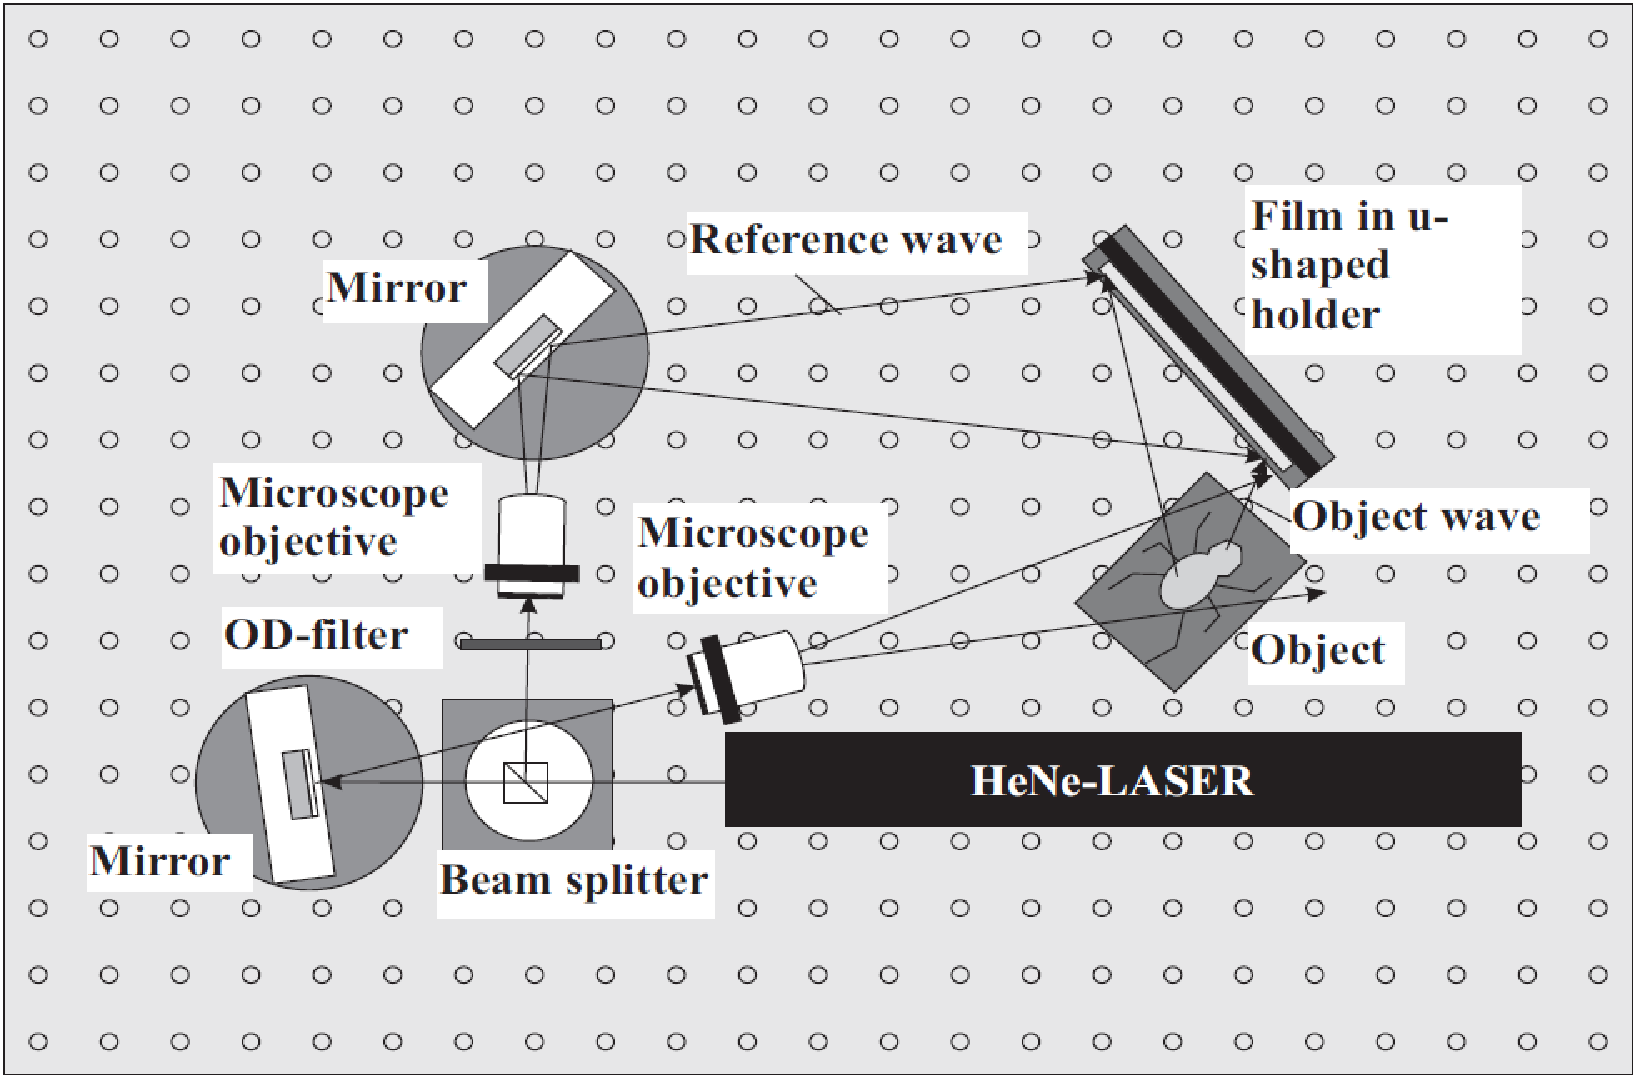
\includegraphics[width=0.5\textwidth]{graphics/aufbau_transmiss}
  \caption{Set-up for taking a transmission hologram}
  \label{fig:aufbau_transmiss}
\end{figure}
First of all one has to consider that the object and the holographic film are illuminated homogeneously. But due to reasons of coherence it is also important that the difference in pathlength of object and reference beam does not exceed approximately $\unit[30]{cm}$. Furthermore one inserts an OD filter into the reference beam to adjust the intensities of both beams. If everything is aligned properly the light is switched off except for a small LED panel and the exposure of the holographic film is done for $\unit[5]{s}$. Then the film is developed like explained in the description~\cite{skript}. For reconstruction of the object the film is placed at its position of recording, the object is removed and the object beam is blocked. Now we are indeed able to observe a three dimensional transmission hologram at the former position of the object (see figure \ref{fig:transmiss}), but the angle range for observation is rather small.
\begin{figure}[H]
    \begin{minipage}{0.2\textheight}
  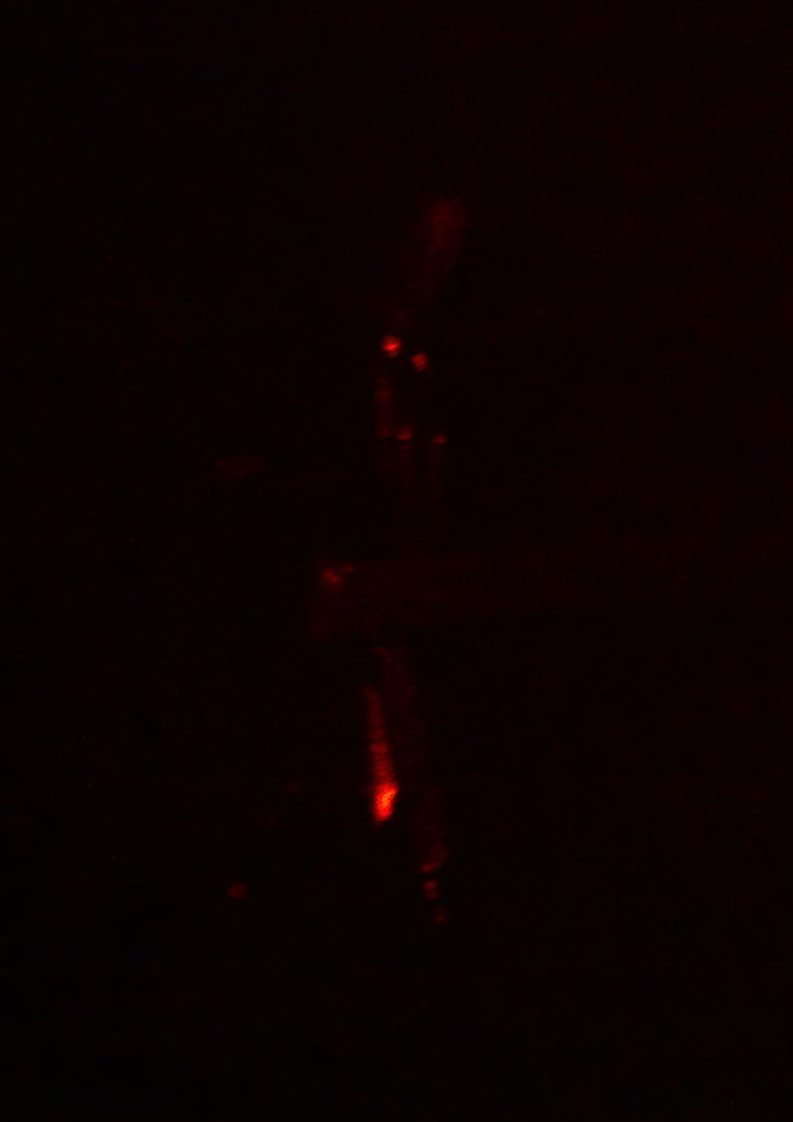
\includegraphics[width=1.0\textwidth]{graphics/transmiss1}
    \end{minipage}
    \hspace{1.3cm}
    \begin{minipage}{0.17\textheight}
  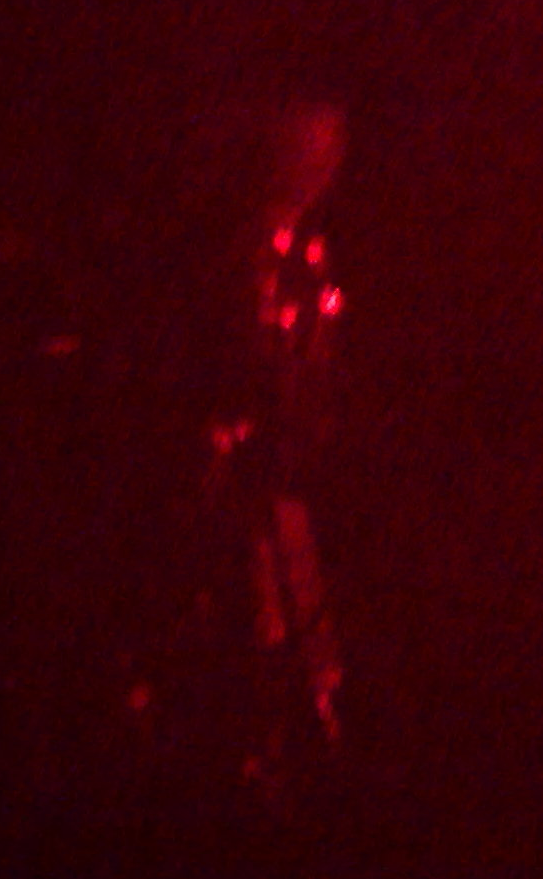
\includegraphics[width=1.0\textwidth]{graphics/transmiss2}
    \end{minipage}
  \caption{Photographs of our transmission hologram}
  \label{fig:transmiss}
\end{figure}
If one uses normal light only a spectral pattern due to the mentioned grating-like structure of the developed film is observed.

\subsection{Reflection Hologram}
The next task is to record a reflection hologram. Again a homogeneous illumination of the holographic plate is important (set-up see figure \ref{fig:aufbau_refl}).
\begin{figure}[H]
  \centering
  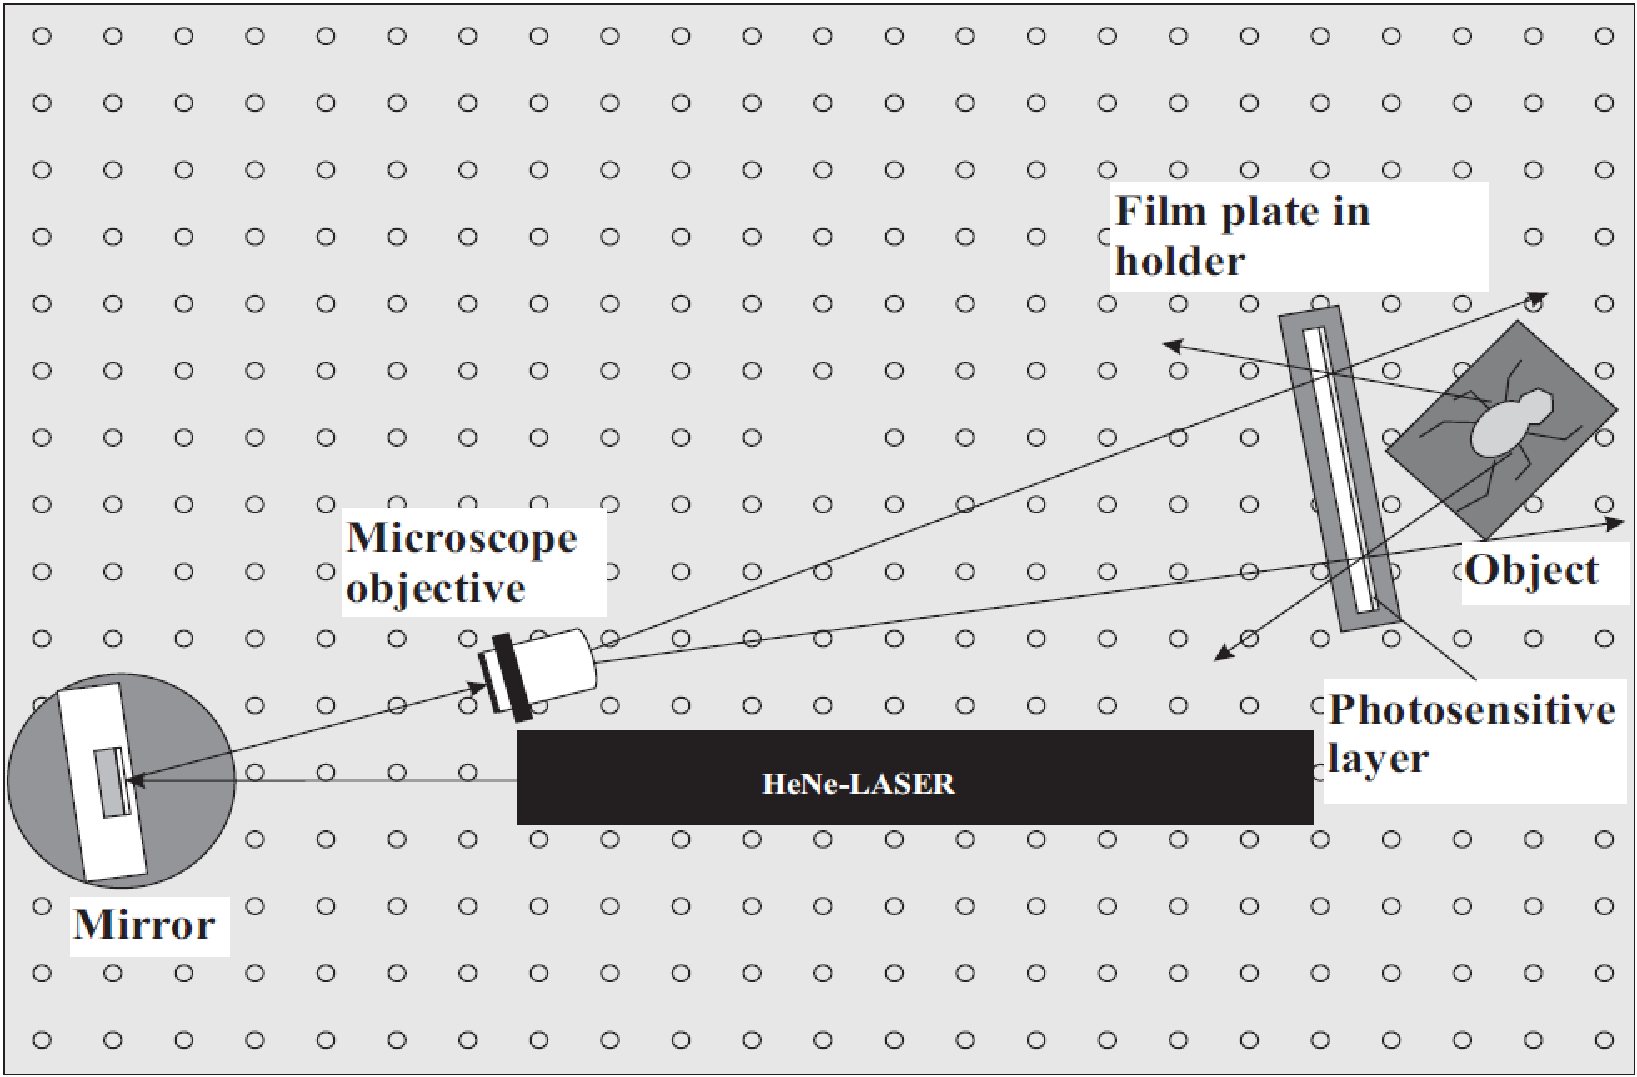
\includegraphics[width=0.5\textwidth]{graphics/aufbau_refl}
  \caption{Set-up for taking a reflection hologram}
  \label{fig:aufbau_refl}
\end{figure}
The object has to be placed behind the holographic plate, whereas the coating points towards the object. The advantage is that the difference in pathlength is minimal and the illumination of the holographic plate has maximal intensity.

With this set-up we take two holograms. While the first one uses a non-processed holographic plate, the other one first of all is treated with an expanding agent. Actually this is done directly at the beginning of the experimentation, because it takes some time to dry. Both are illuminated for about $\unit[8]{s}$ and are then treated as before with respect to developement.

\subsubsection*{Without Expanding Agent}
Unfortunately we missed to remove the OD filter while exposing the film. Therefore our hologram is weaker than it was supposed to be. Therefore it was difficult to compare it with the transmission hologram. The reflection hologram should have a higher intensity and be more detailed than the transmission hologram. Furthermore the angle range of possible observation is expected to be larger. Indeed we could hardly see anything. Besides removing the filter also a longer illumination time could have improved the recording.

\subsubsection*{With Expanding Agent}
Using an expanding agent indeed promises an even better result than simple reflection holography, because after the expansion the coating contracts again such that the lattice constant gets smaller. Therefore it is possible to see the hologram at shorter wavelength. So we expect that it is not possible to reconstruct it with the red laser light we used. Instead it should be possible to observe the hologram with a bulb of high intensity emitting white light, because the \textsc{Bragg} condition will just "choose" the right wavelength as described in section ...\ref{cha:bragg}.... But in practise a big problem arose because of a very long drying time. In fact the expanded plate was not dry after more than 22 hours. We are of the opinion that this should have happened because of wet desiccant. Anyway it of course was not possible to take a holograph with a wet holographic plate. So unfortunately we could not confirm the above mentioned indications.


\subsection{Holography with Lithium Niobate}
\label{subsec:ana_linbo3}
\subsubsection{Recording the Writing Curve}
\label{subsubsec:ana_writing}
In this part of the experiment we want to store a transmission phase hologram in a photorefractive lithium niobate crystal. In oder to do this we set up the experiment as shown in figure \ref{fig:setup_writing}.
\begin{figure}[H]
	\centering
		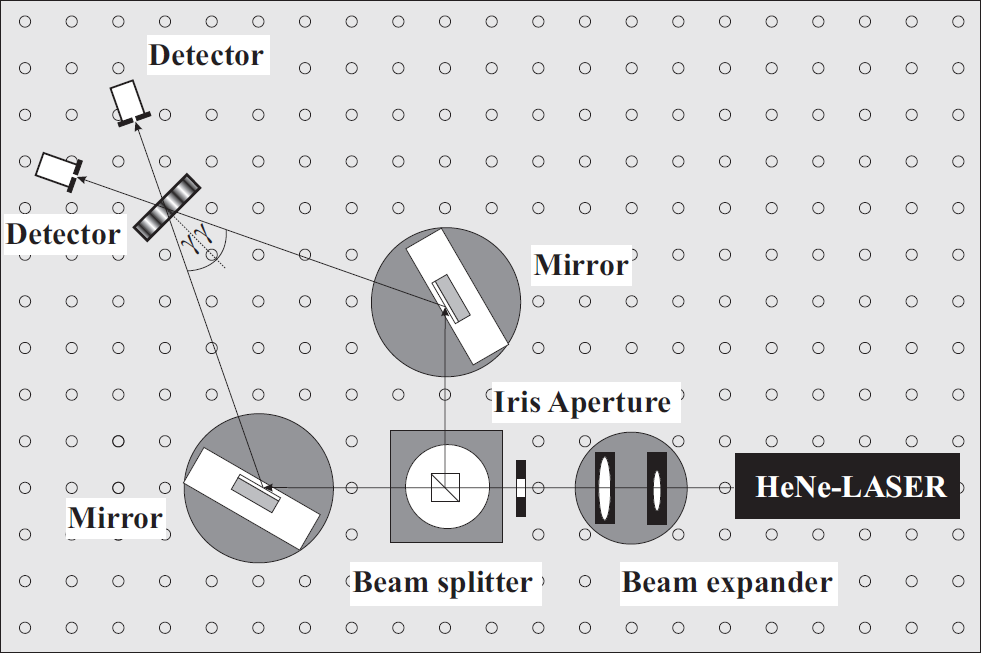
\includegraphics[width=0.5\textwidth]{graphics/setup_writing}
	\caption{Setup for recording the writing curve \cite{skript}}
	\label{fig:setup_writing}
\end{figure}
We adjust the angle between the normal to the recording surface and the writing beams to $\gamma = \unit[(20.0\pm 0.2)]{^\circ}$. Therefore the angle between the two beams inside the crystal is given by the \textsc{Snellius'} law:
\begin{align}
\theta = \arcsin\left(\frac{n_\textrm{Air}}{n_\textrm{crystal}}\sin\gamma\right) = \unit[(8.59 \pm 0.08)]{^\circ}
\end{align}
because the refractive index of the \linbo crystal is given by $n_\textrm{crystal} = \unit[2.29]{}$ for light with a wavelength of $\lambda = \unit[633]{nm}$.
After having optimized the setup we illuminate the crystal with a tungsten lamp for around one hour to erase possibly existing holograms. 

Now we block the laser and perform background measurements for both photodiodes. Because they are connected to an amplifier, we do the measurement for each range. The results are displayed in table \ref{tab:ana_background}. Eventually we are ready to record the writing curve. We unblock the laser and measure the diffraction effiency in time intervalls of about one minute. To measure the intensities we block one of the writing beams so one of the photodiodes measures the diffracted and the other one the transmitted intensity.

\begin{table}[H]
  \centering
\resizebox{0.5\textwidth}{!}{
  \begin{tabular}{l|cc}
    \toprule
     Range & $I_\textrm{diff}^\textrm{bgd}$ [$\unit[]{mW}$] & $I_\textrm{trans}^\textrm{bgd}$ [$\unit[]{mW}$]\\
    \midrule[0.75pt]
$3$ & $-4.0 \pm 0.5$ & $0.0 \pm 0.5$\\
$4$ & $-4.0 \pm 0.5$ & $0.0 \pm 0.5$\\
$5$ & $-4.0 \pm 0.5$ & $0.0 \pm 0.5$\\
$6$ & $-4.0 \pm 0.5$ & $0.0 \pm 0.5$\\
$7$ & $-2.0 \pm 0.5$ & $2.0 \pm 0.5$\\
$8$ & $17.0 \pm 0.5$ & $25.0 \pm 0.5$\\
    \bottomrule
  \end{tabular}
}
\caption{Background measurements for the two photodiodes}
  \label{tab:ana_background}
\end{table}

The first curve we recorded this way behaved well for the first 20 minutes, but then began contrary to our expectation to fall again.  This was most likely caused by a reflection hitting the crystal, which then erased the hologram. So we realigned our setup, dropped the data and restarted the measurement. The data is shown in tables \ref{tab:ana_writing_first} and \ref{tab:ana_writing_second} in the appendix and plotted in figure \ref{fig:ana_writing}.
\begin{figure}[H]
\begin{floatrow}
\resizebox{0.5\textwidth}{!}{
	\begin{tikzpicture}[gnuplot]
%% generated with GNUPLOT 4.4p0 (Lua 5.1.4; terminal rev. 97, script rev. 96a)
%% 09.05.2010 23:59:42
\gpcolor{gp lt color border}
\gpsetlinetype{gp lt border}
\gpsetlinewidth{1.00}
\draw[gp path] (1.504,0.985)--(1.684,0.985);
\draw[gp path] (12.039,0.985)--(11.859,0.985);
\node[gp node right] at (1.320,0.985) { 0};
\draw[gp path] (1.504,2.042)--(1.684,2.042);
\draw[gp path] (12.039,2.042)--(11.859,2.042);
\node[gp node right] at (1.320,2.042) { 2};
\draw[gp path] (1.504,3.098)--(1.684,3.098);
\draw[gp path] (12.039,3.098)--(11.859,3.098);
\node[gp node right] at (1.320,3.098) { 4};
\draw[gp path] (1.504,4.155)--(1.684,4.155);
\draw[gp path] (12.039,4.155)--(11.859,4.155);
\node[gp node right] at (1.320,4.155) { 6};
\draw[gp path] (1.504,5.211)--(1.684,5.211);
\draw[gp path] (12.039,5.211)--(11.859,5.211);
\node[gp node right] at (1.320,5.211) { 8};
\draw[gp path] (1.504,6.268)--(1.684,6.268);
\draw[gp path] (12.039,6.268)--(11.859,6.268);
\node[gp node right] at (1.320,6.268) { 10};
\draw[gp path] (1.504,7.324)--(1.684,7.324);
\draw[gp path] (12.039,7.324)--(11.859,7.324);
\node[gp node right] at (1.320,7.324) { 12};
\draw[gp path] (1.504,8.381)--(1.684,8.381);
\draw[gp path] (12.039,8.381)--(11.859,8.381);
\node[gp node right] at (1.320,8.381) { 14};
\draw[gp path] (1.504,0.985)--(1.504,1.165);
\draw[gp path] (1.504,8.381)--(1.504,8.201);
\node[gp node center] at (1.504,0.677) { 0};
\draw[gp path] (3.203,0.985)--(3.203,1.165);
\draw[gp path] (3.203,8.381)--(3.203,8.201);
\node[gp node center] at (3.203,0.677) { 500};
\draw[gp path] (4.902,0.985)--(4.902,1.165);
\draw[gp path] (4.902,8.381)--(4.902,8.201);
\node[gp node center] at (4.902,0.677) { 1000};
\draw[gp path] (6.602,0.985)--(6.602,1.165);
\draw[gp path] (6.602,8.381)--(6.602,8.201);
\node[gp node center] at (6.602,0.677) { 1500};
\draw[gp path] (8.301,0.985)--(8.301,1.165);
\draw[gp path] (8.301,8.381)--(8.301,8.201);
\node[gp node center] at (8.301,0.677) { 2000};
\draw[gp path] (10.000,0.985)--(10.000,1.165);
\draw[gp path] (10.000,8.381)--(10.000,8.201);
\node[gp node center] at (10.000,0.677) { 2500};
\draw[gp path] (11.699,0.985)--(11.699,1.165);
\draw[gp path] (11.699,8.381)--(11.699,8.201);
\node[gp node center] at (11.699,0.677) { 3000};
\draw[gp path] (1.504,8.381)--(1.504,0.985)--(12.039,0.985)--(12.039,8.381)--cycle;
\node[gp node center,rotate=-270] at (0.430,4.683) {$\eta$ [$\unit[]{10^{-3}}$]};
\node[gp node center] at (6.771,0.215) {t [s]};
\node[gp node right] at (10.571,8.047) {Measured Data};
\gpcolor{gp lt color 0}
\gpsetlinetype{gp lt plot 0}
\draw[gp path] (10.755,8.047)--(11.671,8.047);
\draw[gp path] (10.755,8.137)--(10.755,7.957);
\draw[gp path] (11.671,8.137)--(11.671,7.957);
\draw[gp path] (1.504,1.019)--(1.504,1.020);
\draw[gp path] (1.414,1.019)--(1.594,1.019);
\draw[gp path] (1.414,1.020)--(1.594,1.020);
\draw[gp path] (1.636,1.044)--(1.816,1.044);
\draw[gp path] (1.636,1.044)--(1.816,1.044);
\draw[gp path] (1.948,1.091)--(1.948,1.092);
\draw[gp path] (1.858,1.091)--(2.038,1.091);
\draw[gp path] (1.858,1.092)--(2.038,1.092);
\draw[gp path] (2.181,1.115)--(2.181,1.116);
\draw[gp path] (2.091,1.115)--(2.271,1.115);
\draw[gp path] (2.091,1.116)--(2.271,1.116);
\draw[gp path] (2.368,1.150)--(2.368,1.151);
\draw[gp path] (2.278,1.150)--(2.458,1.150);
\draw[gp path] (2.278,1.151)--(2.458,1.151);
\draw[gp path] (2.542,1.191)--(2.542,1.192);
\draw[gp path] (2.452,1.191)--(2.632,1.191);
\draw[gp path] (2.452,1.192)--(2.632,1.192);
\draw[gp path] (2.737,1.233)--(2.737,1.235);
\draw[gp path] (2.647,1.233)--(2.827,1.233);
\draw[gp path] (2.647,1.235)--(2.827,1.235);
\draw[gp path] (2.964,1.263)--(2.964,1.264);
\draw[gp path] (2.874,1.263)--(3.054,1.263);
\draw[gp path] (2.874,1.264)--(3.054,1.264);
\draw[gp path] (3.136,1.315)--(3.136,1.316);
\draw[gp path] (3.046,1.315)--(3.226,1.315);
\draw[gp path] (3.046,1.316)--(3.226,1.316);
\draw[gp path] (3.361,1.364)--(3.361,1.365);
\draw[gp path] (3.271,1.364)--(3.451,1.364);
\draw[gp path] (3.271,1.365)--(3.451,1.365);
\draw[gp path] (3.574,1.419)--(3.574,1.420);
\draw[gp path] (3.484,1.419)--(3.664,1.419);
\draw[gp path] (3.484,1.420)--(3.664,1.420);
\draw[gp path] (3.796,1.468)--(3.796,1.470);
\draw[gp path] (3.706,1.468)--(3.886,1.468);
\draw[gp path] (3.706,1.470)--(3.886,1.470);
\draw[gp path] (3.995,1.536)--(3.995,1.537);
\draw[gp path] (3.905,1.536)--(4.085,1.536);
\draw[gp path] (3.905,1.537)--(4.085,1.537);
\draw[gp path] (4.218,1.590)--(4.218,1.591);
\draw[gp path] (4.128,1.590)--(4.308,1.590);
\draw[gp path] (4.128,1.591)--(4.308,1.591);
\draw[gp path] (4.456,1.640)--(4.456,1.641);
\draw[gp path] (4.366,1.640)--(4.546,1.640);
\draw[gp path] (4.366,1.641)--(4.546,1.641);
\draw[gp path] (4.627,1.710)--(4.627,1.712);
\draw[gp path] (4.537,1.710)--(4.717,1.710);
\draw[gp path] (4.537,1.712)--(4.717,1.712);
\draw[gp path] (4.852,1.766)--(4.852,1.768);
\draw[gp path] (4.762,1.766)--(4.942,1.766);
\draw[gp path] (4.762,1.768)--(4.942,1.768);
\draw[gp path] (5.078,1.830)--(5.078,1.831);
\draw[gp path] (4.988,1.830)--(5.168,1.830);
\draw[gp path] (4.988,1.831)--(5.168,1.831);
\draw[gp path] (5.294,1.898)--(5.294,1.900);
\draw[gp path] (5.204,1.898)--(5.384,1.898);
\draw[gp path] (5.204,1.900)--(5.384,1.900);
\draw[gp path] (5.486,1.981)--(5.486,1.991);
\draw[gp path] (5.396,1.981)--(5.576,1.981);
\draw[gp path] (5.396,1.991)--(5.576,1.991);
\draw[gp path] (5.717,2.064)--(5.717,2.074);
\draw[gp path] (5.627,2.064)--(5.807,2.064);
\draw[gp path] (5.627,2.074)--(5.807,2.074);
\draw[gp path] (5.918,2.142)--(5.918,2.152);
\draw[gp path] (5.828,2.142)--(6.008,2.142);
\draw[gp path] (5.828,2.152)--(6.008,2.152);
\draw[gp path] (6.137,2.225)--(6.137,2.235);
\draw[gp path] (6.047,2.225)--(6.227,2.225);
\draw[gp path] (6.047,2.235)--(6.227,2.235);
\draw[gp path] (6.308,2.300)--(6.308,2.310);
\draw[gp path] (6.218,2.300)--(6.398,2.300);
\draw[gp path] (6.218,2.310)--(6.398,2.310);
\draw[gp path] (6.544,2.400)--(6.544,2.410);
\draw[gp path] (6.454,2.400)--(6.634,2.400);
\draw[gp path] (6.454,2.410)--(6.634,2.410);
\draw[gp path] (6.772,2.483)--(6.772,2.493);
\draw[gp path] (6.682,2.483)--(6.862,2.483);
\draw[gp path] (6.682,2.493)--(6.862,2.493);
\draw[gp path] (6.978,2.596)--(6.978,2.606);
\draw[gp path] (6.888,2.596)--(7.068,2.596);
\draw[gp path] (6.888,2.606)--(7.068,2.606);
\draw[gp path] (7.179,2.710)--(7.179,2.720);
\draw[gp path] (7.089,2.710)--(7.269,2.710);
\draw[gp path] (7.089,2.720)--(7.269,2.720);
\draw[gp path] (7.375,2.831)--(7.375,2.841);
\draw[gp path] (7.285,2.831)--(7.465,2.831);
\draw[gp path] (7.285,2.841)--(7.465,2.841);
\draw[gp path] (7.604,2.951)--(7.604,2.962);
\draw[gp path] (7.514,2.951)--(7.694,2.951);
\draw[gp path] (7.514,2.962)--(7.694,2.962);
\draw[gp path] (7.780,3.105)--(7.780,3.115);
\draw[gp path] (7.690,3.105)--(7.870,3.105);
\draw[gp path] (7.690,3.115)--(7.870,3.115);
\draw[gp path] (7.999,3.229)--(7.999,3.240);
\draw[gp path] (7.909,3.229)--(8.089,3.229);
\draw[gp path] (7.909,3.240)--(8.089,3.240);
\draw[gp path] (8.197,3.367)--(8.197,3.377);
\draw[gp path] (8.107,3.367)--(8.287,3.367);
\draw[gp path] (8.107,3.377)--(8.287,3.377);
\draw[gp path] (8.432,3.534)--(8.432,3.545);
\draw[gp path] (8.342,3.534)--(8.522,3.534);
\draw[gp path] (8.342,3.545)--(8.522,3.545);
\draw[gp path] (8.652,3.691)--(8.652,3.702);
\draw[gp path] (8.562,3.691)--(8.742,3.691);
\draw[gp path] (8.562,3.702)--(8.742,3.702);
\draw[gp path] (8.863,3.835)--(8.863,3.846);
\draw[gp path] (8.773,3.835)--(8.953,3.835);
\draw[gp path] (8.773,3.846)--(8.953,3.846);
\draw[gp path] (9.072,4.025)--(9.072,4.036);
\draw[gp path] (8.982,4.025)--(9.162,4.025);
\draw[gp path] (8.982,4.036)--(9.162,4.036);
\draw[gp path] (9.295,4.214)--(9.295,4.226);
\draw[gp path] (9.205,4.214)--(9.385,4.214);
\draw[gp path] (9.205,4.226)--(9.385,4.226);
\draw[gp path] (9.492,4.384)--(9.492,4.396);
\draw[gp path] (9.402,4.384)--(9.582,4.384);
\draw[gp path] (9.402,4.396)--(9.582,4.396);
\draw[gp path] (9.666,4.576)--(9.666,4.588);
\draw[gp path] (9.576,4.576)--(9.756,4.576);
\draw[gp path] (9.576,4.588)--(9.756,4.588);
\draw[gp path] (9.896,4.801)--(9.896,4.812);
\draw[gp path] (9.806,4.801)--(9.986,4.801);
\draw[gp path] (9.806,4.812)--(9.986,4.812);
\draw[gp path] (10.068,5.029)--(10.068,5.041);
\draw[gp path] (9.978,5.029)--(10.158,5.029);
\draw[gp path] (9.978,5.041)--(10.158,5.041);
\draw[gp path] (10.295,5.250)--(10.295,5.263);
\draw[gp path] (10.205,5.250)--(10.385,5.250);
\draw[gp path] (10.205,5.263)--(10.385,5.263);
\draw[gp path] (10.491,5.490)--(10.491,5.502);
\draw[gp path] (10.401,5.490)--(10.581,5.490);
\draw[gp path] (10.401,5.502)--(10.581,5.502);
\draw[gp path] (10.666,5.770)--(10.666,5.783);
\draw[gp path] (10.576,5.770)--(10.756,5.770);
\draw[gp path] (10.576,5.783)--(10.756,5.783);
\draw[gp path] (10.895,6.026)--(10.895,6.039);
\draw[gp path] (10.805,6.026)--(10.985,6.026);
\draw[gp path] (10.805,6.039)--(10.985,6.039);
\draw[gp path] (11.107,6.288)--(11.107,6.302);
\draw[gp path] (11.017,6.288)--(11.197,6.288);
\draw[gp path] (11.017,6.302)--(11.197,6.302);
\draw[gp path] (11.332,6.595)--(11.332,6.609);
\draw[gp path] (11.242,6.595)--(11.422,6.595);
\draw[gp path] (11.242,6.609)--(11.422,6.609);
\draw[gp path] (11.546,6.865)--(11.546,6.879);
\draw[gp path] (11.456,6.865)--(11.636,6.865);
\draw[gp path] (11.456,6.879)--(11.636,6.879);
\draw[gp path] (11.727,7.174)--(11.727,7.189);
\draw[gp path] (11.637,7.174)--(11.817,7.174);
\draw[gp path] (11.637,7.189)--(11.817,7.189);
\draw[gp path] (11.907,7.452)--(11.907,7.467);
\draw[gp path] (11.817,7.452)--(11.997,7.452);
\draw[gp path] (11.817,7.467)--(11.997,7.467);
\draw[gp path] (1.504,1.019)--(1.506,1.019);
\draw[gp path] (1.504,0.929)--(1.504,1.109);
\draw[gp path] (1.506,0.929)--(1.506,1.109);
\draw[gp path] (1.724,1.044)--(1.728,1.044);
\draw[gp path] (1.724,0.954)--(1.724,1.134);
\draw[gp path] (1.728,0.954)--(1.728,1.134);
\draw[gp path] (1.946,1.091)--(1.949,1.091);
\draw[gp path] (1.946,1.001)--(1.946,1.181);
\draw[gp path] (1.949,1.001)--(1.949,1.181);
\draw[gp path] (2.179,1.115)--(2.183,1.115);
\draw[gp path] (2.179,1.025)--(2.179,1.205);
\draw[gp path] (2.183,1.025)--(2.183,1.205);
\draw[gp path] (2.366,1.151)--(2.370,1.151);
\draw[gp path] (2.366,1.061)--(2.366,1.241);
\draw[gp path] (2.370,1.061)--(2.370,1.241);
\draw[gp path] (2.540,1.191)--(2.543,1.191);
\draw[gp path] (2.540,1.101)--(2.540,1.281);
\draw[gp path] (2.543,1.101)--(2.543,1.281);
\draw[gp path] (2.735,1.234)--(2.739,1.234);
\draw[gp path] (2.735,1.144)--(2.735,1.324);
\draw[gp path] (2.739,1.144)--(2.739,1.324);
\draw[gp path] (2.962,1.263)--(2.965,1.263);
\draw[gp path] (2.962,1.173)--(2.962,1.353);
\draw[gp path] (2.965,1.173)--(2.965,1.353);
\draw[gp path] (3.135,1.315)--(3.138,1.315);
\draw[gp path] (3.135,1.225)--(3.135,1.405);
\draw[gp path] (3.138,1.225)--(3.138,1.405);
\draw[gp path] (3.359,1.364)--(3.363,1.364);
\draw[gp path] (3.359,1.274)--(3.359,1.454);
\draw[gp path] (3.363,1.274)--(3.363,1.454);
\draw[gp path] (3.572,1.419)--(3.575,1.419);
\draw[gp path] (3.572,1.329)--(3.572,1.509);
\draw[gp path] (3.575,1.329)--(3.575,1.509);
\draw[gp path] (3.794,1.469)--(3.797,1.469);
\draw[gp path] (3.794,1.379)--(3.794,1.559);
\draw[gp path] (3.797,1.379)--(3.797,1.559);
\draw[gp path] (3.993,1.537)--(3.997,1.537);
\draw[gp path] (3.993,1.447)--(3.993,1.627);
\draw[gp path] (3.997,1.447)--(3.997,1.627);
\draw[gp path] (4.217,1.590)--(4.220,1.590);
\draw[gp path] (4.217,1.500)--(4.217,1.680);
\draw[gp path] (4.220,1.500)--(4.220,1.680);
\draw[gp path] (4.454,1.640)--(4.458,1.640);
\draw[gp path] (4.454,1.550)--(4.454,1.730);
\draw[gp path] (4.458,1.550)--(4.458,1.730);
\draw[gp path] (4.625,1.711)--(4.628,1.711);
\draw[gp path] (4.625,1.621)--(4.625,1.801);
\draw[gp path] (4.628,1.621)--(4.628,1.801);
\draw[gp path] (4.850,1.767)--(4.854,1.767);
\draw[gp path] (4.850,1.677)--(4.850,1.857);
\draw[gp path] (4.854,1.677)--(4.854,1.857);
\draw[gp path] (5.077,1.831)--(5.080,1.831);
\draw[gp path] (5.077,1.741)--(5.077,1.921);
\draw[gp path] (5.080,1.741)--(5.080,1.921);
\draw[gp path] (5.292,1.899)--(5.295,1.899);
\draw[gp path] (5.292,1.809)--(5.292,1.989);
\draw[gp path] (5.295,1.809)--(5.295,1.989);
\draw[gp path] (5.484,1.986)--(5.488,1.986);
\draw[gp path] (5.484,1.896)--(5.484,2.076);
\draw[gp path] (5.488,1.896)--(5.488,2.076);
\draw[gp path] (5.715,2.069)--(5.718,2.069);
\draw[gp path] (5.715,1.979)--(5.715,2.159);
\draw[gp path] (5.718,1.979)--(5.718,2.159);
\draw[gp path] (5.916,2.147)--(5.920,2.147);
\draw[gp path] (5.916,2.057)--(5.916,2.237);
\draw[gp path] (5.920,2.057)--(5.920,2.237);
\draw[gp path] (6.135,2.230)--(6.138,2.230);
\draw[gp path] (6.135,2.140)--(6.135,2.320);
\draw[gp path] (6.138,2.140)--(6.138,2.320);
\draw[gp path] (6.306,2.305)--(6.310,2.305);
\draw[gp path] (6.306,2.215)--(6.306,2.395);
\draw[gp path] (6.310,2.215)--(6.310,2.395);
\draw[gp path] (6.543,2.405)--(6.546,2.405);
\draw[gp path] (6.543,2.315)--(6.543,2.495);
\draw[gp path] (6.546,2.315)--(6.546,2.495);
\draw[gp path] (6.770,2.488)--(6.774,2.488);
\draw[gp path] (6.770,2.398)--(6.770,2.578);
\draw[gp path] (6.774,2.398)--(6.774,2.578);
\draw[gp path] (6.976,2.601)--(6.980,2.601);
\draw[gp path] (6.976,2.511)--(6.976,2.691);
\draw[gp path] (6.980,2.511)--(6.980,2.691);
\draw[gp path] (7.177,2.715)--(7.181,2.715);
\draw[gp path] (7.177,2.625)--(7.177,2.805);
\draw[gp path] (7.181,2.625)--(7.181,2.805);
\draw[gp path] (7.373,2.836)--(7.376,2.836);
\draw[gp path] (7.373,2.746)--(7.373,2.926);
\draw[gp path] (7.376,2.746)--(7.376,2.926);
\draw[gp path] (7.603,2.956)--(7.606,2.956);
\draw[gp path] (7.603,2.866)--(7.603,3.046);
\draw[gp path] (7.606,2.866)--(7.606,3.046);
\draw[gp path] (7.778,3.110)--(7.782,3.110);
\draw[gp path] (7.778,3.020)--(7.778,3.200);
\draw[gp path] (7.782,3.020)--(7.782,3.200);
\draw[gp path] (7.998,3.235)--(8.001,3.235);
\draw[gp path] (7.998,3.145)--(7.998,3.325);
\draw[gp path] (8.001,3.145)--(8.001,3.325);
\draw[gp path] (8.195,3.372)--(8.199,3.372);
\draw[gp path] (8.195,3.282)--(8.195,3.462);
\draw[gp path] (8.199,3.282)--(8.199,3.462);
\draw[gp path] (8.430,3.539)--(8.434,3.539);
\draw[gp path] (8.430,3.449)--(8.430,3.629);
\draw[gp path] (8.434,3.449)--(8.434,3.629);
\draw[gp path] (8.650,3.697)--(8.654,3.697);
\draw[gp path] (8.650,3.607)--(8.650,3.787);
\draw[gp path] (8.654,3.607)--(8.654,3.787);
\draw[gp path] (8.861,3.841)--(8.865,3.841);
\draw[gp path] (8.861,3.751)--(8.861,3.931);
\draw[gp path] (8.865,3.751)--(8.865,3.931);
\draw[gp path] (9.070,4.031)--(9.073,4.031);
\draw[gp path] (9.070,3.941)--(9.070,4.121);
\draw[gp path] (9.073,3.941)--(9.073,4.121);
\draw[gp path] (9.293,4.220)--(9.296,4.220);
\draw[gp path] (9.293,4.130)--(9.293,4.310);
\draw[gp path] (9.296,4.130)--(9.296,4.310);
\draw[gp path] (9.490,4.390)--(9.494,4.390);
\draw[gp path] (9.490,4.300)--(9.490,4.480);
\draw[gp path] (9.494,4.300)--(9.494,4.480);
\draw[gp path] (9.664,4.582)--(9.668,4.582);
\draw[gp path] (9.664,4.492)--(9.664,4.672);
\draw[gp path] (9.668,4.492)--(9.668,4.672);
\draw[gp path] (9.894,4.806)--(9.898,4.806);
\draw[gp path] (9.894,4.716)--(9.894,4.896);
\draw[gp path] (9.898,4.716)--(9.898,4.896);
\draw[gp path] (10.067,5.035)--(10.070,5.035);
\draw[gp path] (10.067,4.945)--(10.067,5.125);
\draw[gp path] (10.070,4.945)--(10.070,5.125);
\draw[gp path] (10.293,5.257)--(10.297,5.257);
\draw[gp path] (10.293,5.167)--(10.293,5.347);
\draw[gp path] (10.297,5.167)--(10.297,5.347);
\draw[gp path] (10.489,5.496)--(10.493,5.496);
\draw[gp path] (10.489,5.406)--(10.489,5.586);
\draw[gp path] (10.493,5.406)--(10.493,5.586);
\draw[gp path] (10.664,5.776)--(10.668,5.776);
\draw[gp path] (10.664,5.686)--(10.664,5.866);
\draw[gp path] (10.668,5.686)--(10.668,5.866);
\draw[gp path] (10.894,6.032)--(10.897,6.032);
\draw[gp path] (10.894,5.942)--(10.894,6.122);
\draw[gp path] (10.897,5.942)--(10.897,6.122);
\draw[gp path] (11.105,6.295)--(11.109,6.295);
\draw[gp path] (11.105,6.205)--(11.105,6.385);
\draw[gp path] (11.109,6.205)--(11.109,6.385);
\draw[gp path] (11.331,6.602)--(11.334,6.602);
\draw[gp path] (11.331,6.512)--(11.331,6.692);
\draw[gp path] (11.334,6.512)--(11.334,6.692);
\draw[gp path] (11.544,6.872)--(11.547,6.872);
\draw[gp path] (11.544,6.782)--(11.544,6.962);
\draw[gp path] (11.547,6.782)--(11.547,6.962);
\draw[gp path] (11.725,7.181)--(11.728,7.181);
\draw[gp path] (11.725,7.091)--(11.725,7.271);
\draw[gp path] (11.728,7.091)--(11.728,7.271);
\draw[gp path] (11.905,7.459)--(11.909,7.459);
\draw[gp path] (11.905,7.369)--(11.905,7.549);
\draw[gp path] (11.909,7.369)--(11.909,7.549);
\gpsetpointsize{4.00}
\gppoint{gp mark 1}{(1.504,1.019)}
\gppoint{gp mark 1}{(1.726,1.044)}
\gppoint{gp mark 1}{(1.948,1.091)}
\gppoint{gp mark 1}{(2.181,1.115)}
\gppoint{gp mark 1}{(2.368,1.151)}
\gppoint{gp mark 1}{(2.542,1.191)}
\gppoint{gp mark 1}{(2.737,1.234)}
\gppoint{gp mark 1}{(2.964,1.263)}
\gppoint{gp mark 1}{(3.136,1.315)}
\gppoint{gp mark 1}{(3.361,1.364)}
\gppoint{gp mark 1}{(3.574,1.419)}
\gppoint{gp mark 1}{(3.796,1.469)}
\gppoint{gp mark 1}{(3.995,1.537)}
\gppoint{gp mark 1}{(4.218,1.590)}
\gppoint{gp mark 1}{(4.456,1.640)}
\gppoint{gp mark 1}{(4.627,1.711)}
\gppoint{gp mark 1}{(4.852,1.767)}
\gppoint{gp mark 1}{(5.078,1.831)}
\gppoint{gp mark 1}{(5.294,1.899)}
\gppoint{gp mark 1}{(5.486,1.986)}
\gppoint{gp mark 1}{(5.717,2.069)}
\gppoint{gp mark 1}{(5.918,2.147)}
\gppoint{gp mark 1}{(6.137,2.230)}
\gppoint{gp mark 1}{(6.308,2.305)}
\gppoint{gp mark 1}{(6.544,2.405)}
\gppoint{gp mark 1}{(6.772,2.488)}
\gppoint{gp mark 1}{(6.978,2.601)}
\gppoint{gp mark 1}{(7.179,2.715)}
\gppoint{gp mark 1}{(7.375,2.836)}
\gppoint{gp mark 1}{(7.604,2.956)}
\gppoint{gp mark 1}{(7.780,3.110)}
\gppoint{gp mark 1}{(7.999,3.235)}
\gppoint{gp mark 1}{(8.197,3.372)}
\gppoint{gp mark 1}{(8.432,3.539)}
\gppoint{gp mark 1}{(8.652,3.697)}
\gppoint{gp mark 1}{(8.863,3.841)}
\gppoint{gp mark 1}{(9.072,4.031)}
\gppoint{gp mark 1}{(9.295,4.220)}
\gppoint{gp mark 1}{(9.492,4.390)}
\gppoint{gp mark 1}{(9.666,4.582)}
\gppoint{gp mark 1}{(9.896,4.806)}
\gppoint{gp mark 1}{(10.068,5.035)}
\gppoint{gp mark 1}{(10.295,5.257)}
\gppoint{gp mark 1}{(10.491,5.496)}
\gppoint{gp mark 1}{(10.666,5.776)}
\gppoint{gp mark 1}{(10.895,6.032)}
\gppoint{gp mark 1}{(11.107,6.295)}
\gppoint{gp mark 1}{(11.332,6.602)}
\gppoint{gp mark 1}{(11.546,6.872)}
\gppoint{gp mark 1}{(11.727,7.181)}
\gppoint{gp mark 1}{(11.907,7.459)}
\gppoint{gp mark 1}{(11.213,8.047)}
\gpcolor{gp lt color border}
\gpsetlinetype{gp lt border}
\draw[gp path] (1.504,8.381)--(1.504,0.985)--(12.039,0.985)--(12.039,8.381)--cycle;
%% coordinates of the plot area
\gpdefrectangularnode{gp plot 1}{\pgfpoint{1.504cm}{0.985cm}}{\pgfpoint{12.039cm}{8.381cm}}
\end{tikzpicture}
%% gnuplot variables

}
\resizebox{0.5\textwidth}{!}{
	\begin{tikzpicture}[gnuplot]
%% generated with GNUPLOT 4.4p0 (Lua 5.1.4; terminal rev. 97, script rev. 96a)
%% 09.05.2010 23:59:42
\gpcolor{gp lt color border}
\gpsetlinetype{gp lt border}
\gpsetlinewidth{1.00}
\draw[gp path] (1.688,0.985)--(1.868,0.985);
\draw[gp path] (12.039,0.985)--(11.859,0.985);
\node[gp node right] at (1.504,0.985) { 0};
\draw[gp path] (1.688,2.218)--(1.868,2.218);
\draw[gp path] (12.039,2.218)--(11.859,2.218);
\node[gp node right] at (1.504,2.218) { 20};
\draw[gp path] (1.688,3.450)--(1.868,3.450);
\draw[gp path] (12.039,3.450)--(11.859,3.450);
\node[gp node right] at (1.504,3.450) { 40};
\draw[gp path] (1.688,4.683)--(1.868,4.683);
\draw[gp path] (12.039,4.683)--(11.859,4.683);
\node[gp node right] at (1.504,4.683) { 60};
\draw[gp path] (1.688,5.916)--(1.868,5.916);
\draw[gp path] (12.039,5.916)--(11.859,5.916);
\node[gp node right] at (1.504,5.916) { 80};
\draw[gp path] (1.688,7.148)--(1.868,7.148);
\draw[gp path] (12.039,7.148)--(11.859,7.148);
\node[gp node right] at (1.504,7.148) { 100};
\draw[gp path] (1.688,8.381)--(1.868,8.381);
\draw[gp path] (12.039,8.381)--(11.859,8.381);
\node[gp node right] at (1.504,8.381) { 120};
\draw[gp path] (1.688,0.985)--(1.688,1.165);
\draw[gp path] (1.688,8.381)--(1.688,8.201);
\node[gp node center] at (1.688,0.677) { 0};
\draw[gp path] (3.358,0.985)--(3.358,1.165);
\draw[gp path] (3.358,8.381)--(3.358,8.201);
\node[gp node center] at (3.358,0.677) { 500};
\draw[gp path] (5.027,0.985)--(5.027,1.165);
\draw[gp path] (5.027,8.381)--(5.027,8.201);
\node[gp node center] at (5.027,0.677) { 1000};
\draw[gp path] (6.697,0.985)--(6.697,1.165);
\draw[gp path] (6.697,8.381)--(6.697,8.201);
\node[gp node center] at (6.697,0.677) { 1500};
\draw[gp path] (8.366,0.985)--(8.366,1.165);
\draw[gp path] (8.366,8.381)--(8.366,8.201);
\node[gp node center] at (8.366,0.677) { 2000};
\draw[gp path] (10.036,0.985)--(10.036,1.165);
\draw[gp path] (10.036,8.381)--(10.036,8.201);
\node[gp node center] at (10.036,0.677) { 2500};
\draw[gp path] (11.705,0.985)--(11.705,1.165);
\draw[gp path] (11.705,8.381)--(11.705,8.201);
\node[gp node center] at (11.705,0.677) { 3000};
\draw[gp path] (1.688,8.381)--(1.688,0.985)--(12.039,0.985)--(12.039,8.381)--cycle;
\node[gp node center,rotate=-270] at (0.430,4.683) {$\Delta n$ [$\unit[]{10^{-7}}$]};
\node[gp node center] at (6.863,0.215) {t [s]};
\node[gp node right] at (10.571,8.047) {Measured Data};
\gpcolor{gp lt color 0}
\gpsetlinetype{gp lt plot 0}
\draw[gp path] (10.755,8.047)--(11.671,8.047);
\draw[gp path] (10.755,8.137)--(10.755,7.957);
\draw[gp path] (11.671,8.137)--(11.671,7.957);
\draw[gp path] (1.688,1.480)--(1.688,1.481);
\draw[gp path] (1.598,1.480)--(1.778,1.480);
\draw[gp path] (1.598,1.481)--(1.778,1.481);
\draw[gp path] (1.906,1.633)--(1.906,1.634);
\draw[gp path] (1.816,1.633)--(1.996,1.633);
\draw[gp path] (1.816,1.634)--(1.996,1.634);
\draw[gp path] (2.124,1.855)--(2.124,1.859);
\draw[gp path] (2.034,1.855)--(2.214,1.855);
\draw[gp path] (2.034,1.859)--(2.214,1.859);
\draw[gp path] (2.353,1.946)--(2.353,1.950);
\draw[gp path] (2.263,1.946)--(2.443,1.946);
\draw[gp path] (2.263,1.950)--(2.443,1.950);
\draw[gp path] (2.537,2.071)--(2.537,2.074);
\draw[gp path] (2.447,2.071)--(2.627,2.071);
\draw[gp path] (2.447,2.074)--(2.627,2.074);
\draw[gp path] (2.708,2.196)--(2.708,2.199);
\draw[gp path] (2.618,2.196)--(2.798,2.196);
\draw[gp path] (2.618,2.199)--(2.798,2.199);
\draw[gp path] (2.899,2.317)--(2.899,2.319);
\draw[gp path] (2.809,2.317)--(2.989,2.317);
\draw[gp path] (2.809,2.319)--(2.989,2.319);
\draw[gp path] (3.122,2.393)--(3.122,2.396);
\draw[gp path] (3.032,2.393)--(3.212,2.393);
\draw[gp path] (3.032,2.396)--(3.212,2.396);
\draw[gp path] (3.292,2.519)--(3.292,2.522);
\draw[gp path] (3.202,2.519)--(3.382,2.519);
\draw[gp path] (3.202,2.522)--(3.382,2.522);
\draw[gp path] (3.513,2.629)--(3.513,2.632);
\draw[gp path] (3.423,2.629)--(3.603,2.629);
\draw[gp path] (3.423,2.632)--(3.603,2.632);
\draw[gp path] (3.721,2.745)--(3.721,2.747);
\draw[gp path] (3.631,2.745)--(3.811,2.745);
\draw[gp path] (3.631,2.747)--(3.811,2.747);
\draw[gp path] (3.940,2.842)--(3.940,2.845);
\draw[gp path] (3.850,2.842)--(4.030,2.842);
\draw[gp path] (3.850,2.845)--(4.030,2.845);
\draw[gp path] (4.135,2.968)--(4.135,2.970);
\draw[gp path] (4.045,2.968)--(4.225,2.968);
\draw[gp path] (4.045,2.970)--(4.225,2.970);
\draw[gp path] (4.355,3.063)--(4.355,3.065);
\draw[gp path] (4.265,3.063)--(4.445,3.063);
\draw[gp path] (4.265,3.065)--(4.445,3.065);
\draw[gp path] (4.588,3.147)--(4.588,3.149);
\draw[gp path] (4.498,3.147)--(4.678,3.147);
\draw[gp path] (4.498,3.149)--(4.678,3.149);
\draw[gp path] (4.756,3.260)--(4.756,3.262);
\draw[gp path] (4.666,3.260)--(4.846,3.260);
\draw[gp path] (4.666,3.262)--(4.846,3.262);
\draw[gp path] (4.978,3.346)--(4.978,3.349);
\draw[gp path] (4.888,3.346)--(5.068,3.346);
\draw[gp path] (4.888,3.349)--(5.068,3.349);
\draw[gp path] (5.200,3.440)--(5.200,3.443);
\draw[gp path] (5.110,3.440)--(5.290,3.440);
\draw[gp path] (5.110,3.443)--(5.290,3.443);
\draw[gp path] (5.412,3.538)--(5.412,3.541);
\draw[gp path] (5.322,3.538)--(5.502,3.538);
\draw[gp path] (5.322,3.541)--(5.502,3.541);
\draw[gp path] (5.601,3.651)--(5.601,3.665);
\draw[gp path] (5.511,3.651)--(5.691,3.651);
\draw[gp path] (5.511,3.665)--(5.691,3.665);
\draw[gp path] (5.827,3.761)--(5.827,3.773);
\draw[gp path] (5.737,3.761)--(5.917,3.761);
\draw[gp path] (5.737,3.773)--(5.917,3.773);
\draw[gp path] (6.025,3.859)--(6.025,3.871);
\draw[gp path] (5.935,3.859)--(6.115,3.859);
\draw[gp path] (5.935,3.871)--(6.115,3.871);
\draw[gp path] (6.240,3.960)--(6.240,3.972);
\draw[gp path] (6.150,3.960)--(6.330,3.960);
\draw[gp path] (6.150,3.972)--(6.330,3.972);
\draw[gp path] (6.408,4.049)--(6.408,4.060);
\draw[gp path] (6.318,4.049)--(6.498,4.049);
\draw[gp path] (6.318,4.060)--(6.498,4.060);
\draw[gp path] (6.640,4.164)--(6.640,4.175);
\draw[gp path] (6.550,4.164)--(6.730,4.164);
\draw[gp path] (6.550,4.175)--(6.730,4.175);
\draw[gp path] (6.864,4.255)--(6.864,4.266);
\draw[gp path] (6.774,4.255)--(6.954,4.255);
\draw[gp path] (6.774,4.266)--(6.954,4.266);
\draw[gp path] (7.066,4.377)--(7.066,4.388);
\draw[gp path] (6.976,4.377)--(7.156,4.377);
\draw[gp path] (6.976,4.388)--(7.156,4.388);
\draw[gp path] (7.264,4.495)--(7.264,4.506);
\draw[gp path] (7.174,4.495)--(7.354,4.495);
\draw[gp path] (7.174,4.506)--(7.354,4.506);
\draw[gp path] (7.456,4.616)--(7.456,4.626);
\draw[gp path] (7.366,4.616)--(7.546,4.616);
\draw[gp path] (7.366,4.626)--(7.546,4.626);
\draw[gp path] (7.682,4.733)--(7.682,4.743);
\draw[gp path] (7.592,4.733)--(7.772,4.733);
\draw[gp path] (7.592,4.743)--(7.772,4.743);
\draw[gp path] (7.854,4.877)--(7.854,4.886);
\draw[gp path] (7.764,4.877)--(7.944,4.877);
\draw[gp path] (7.764,4.886)--(7.944,4.886);
\draw[gp path] (8.070,4.989)--(8.070,4.999);
\draw[gp path] (7.980,4.989)--(8.160,4.989);
\draw[gp path] (7.980,4.999)--(8.160,4.999);
\draw[gp path] (8.264,5.110)--(8.264,5.119);
\draw[gp path] (8.174,5.110)--(8.354,5.110);
\draw[gp path] (8.174,5.119)--(8.354,5.119);
\draw[gp path] (8.495,5.253)--(8.495,5.262);
\draw[gp path] (8.405,5.253)--(8.585,5.253);
\draw[gp path] (8.405,5.262)--(8.585,5.262);
\draw[gp path] (8.711,5.383)--(8.711,5.392);
\draw[gp path] (8.621,5.383)--(8.801,5.383);
\draw[gp path] (8.621,5.392)--(8.801,5.392);
\draw[gp path] (8.919,5.499)--(8.919,5.507);
\draw[gp path] (8.829,5.499)--(9.009,5.499);
\draw[gp path] (8.829,5.507)--(9.009,5.507);
\draw[gp path] (9.124,5.647)--(9.124,5.655);
\draw[gp path] (9.034,5.647)--(9.214,5.647);
\draw[gp path] (9.034,5.655)--(9.214,5.655);
\draw[gp path] (9.343,5.790)--(9.343,5.798);
\draw[gp path] (9.253,5.790)--(9.433,5.790);
\draw[gp path] (9.253,5.798)--(9.433,5.798);
\draw[gp path] (9.536,5.915)--(9.536,5.923);
\draw[gp path] (9.446,5.915)--(9.626,5.915);
\draw[gp path] (9.446,5.923)--(9.626,5.923);
\draw[gp path] (9.707,6.053)--(9.707,6.061);
\draw[gp path] (9.617,6.053)--(9.797,6.053);
\draw[gp path] (9.617,6.061)--(9.797,6.061);
\draw[gp path] (9.934,6.209)--(9.934,6.217);
\draw[gp path] (9.844,6.209)--(10.024,6.209);
\draw[gp path] (9.844,6.217)--(10.024,6.217);
\draw[gp path] (10.103,6.364)--(10.103,6.372);
\draw[gp path] (10.013,6.364)--(10.193,6.364);
\draw[gp path] (10.013,6.372)--(10.193,6.372);
\draw[gp path] (10.326,6.509)--(10.326,6.517);
\draw[gp path] (10.236,6.509)--(10.416,6.509);
\draw[gp path] (10.236,6.517)--(10.416,6.517);
\draw[gp path] (10.518,6.662)--(10.518,6.670);
\draw[gp path] (10.428,6.662)--(10.608,6.662);
\draw[gp path] (10.428,6.670)--(10.608,6.670);
\draw[gp path] (10.690,6.837)--(10.690,6.845);
\draw[gp path] (10.600,6.837)--(10.780,6.837);
\draw[gp path] (10.600,6.845)--(10.780,6.845);
\draw[gp path] (10.915,6.992)--(10.915,7.000);
\draw[gp path] (10.825,6.992)--(11.005,6.992);
\draw[gp path] (10.825,7.000)--(11.005,7.000);
\draw[gp path] (11.123,7.146)--(11.123,7.154);
\draw[gp path] (11.033,7.146)--(11.213,7.146);
\draw[gp path] (11.033,7.154)--(11.213,7.154);
\draw[gp path] (11.345,7.323)--(11.345,7.331);
\draw[gp path] (11.255,7.323)--(11.435,7.323);
\draw[gp path] (11.255,7.331)--(11.435,7.331);
\draw[gp path] (11.554,7.474)--(11.554,7.482);
\draw[gp path] (11.464,7.474)--(11.644,7.474);
\draw[gp path] (11.464,7.482)--(11.644,7.482);
\draw[gp path] (11.732,7.643)--(11.732,7.651);
\draw[gp path] (11.642,7.643)--(11.822,7.643);
\draw[gp path] (11.642,7.651)--(11.822,7.651);
\draw[gp path] (11.909,7.792)--(11.909,7.800);
\draw[gp path] (11.819,7.792)--(11.999,7.792);
\draw[gp path] (11.819,7.800)--(11.999,7.800);
\draw[gp path] (1.688,1.481)--(1.690,1.481);
\draw[gp path] (1.688,1.391)--(1.688,1.571);
\draw[gp path] (1.690,1.391)--(1.690,1.571);
\draw[gp path] (1.904,1.633)--(1.908,1.633);
\draw[gp path] (1.904,1.543)--(1.904,1.723);
\draw[gp path] (1.908,1.543)--(1.908,1.723);
\draw[gp path] (2.122,1.857)--(2.126,1.857);
\draw[gp path] (2.122,1.767)--(2.122,1.947);
\draw[gp path] (2.126,1.767)--(2.126,1.947);
\draw[gp path] (2.352,1.948)--(2.355,1.948);
\draw[gp path] (2.352,1.858)--(2.352,2.038);
\draw[gp path] (2.355,1.858)--(2.355,2.038);
\draw[gp path] (2.535,2.073)--(2.538,2.073);
\draw[gp path] (2.535,1.983)--(2.535,2.163);
\draw[gp path] (2.538,1.983)--(2.538,2.163);
\draw[gp path] (2.706,2.198)--(2.709,2.198);
\draw[gp path] (2.706,2.108)--(2.706,2.288);
\draw[gp path] (2.709,2.108)--(2.709,2.288);
\draw[gp path] (2.898,2.318)--(2.901,2.318);
\draw[gp path] (2.898,2.228)--(2.898,2.408);
\draw[gp path] (2.901,2.228)--(2.901,2.408);
\draw[gp path] (3.121,2.394)--(3.124,2.394);
\draw[gp path] (3.121,2.304)--(3.121,2.484);
\draw[gp path] (3.124,2.304)--(3.124,2.484);
\draw[gp path] (3.290,2.520)--(3.293,2.520);
\draw[gp path] (3.290,2.430)--(3.290,2.610);
\draw[gp path] (3.293,2.430)--(3.293,2.610);
\draw[gp path] (3.511,2.630)--(3.514,2.630);
\draw[gp path] (3.511,2.540)--(3.511,2.720);
\draw[gp path] (3.514,2.540)--(3.514,2.720);
\draw[gp path] (3.720,2.746)--(3.723,2.746);
\draw[gp path] (3.720,2.656)--(3.720,2.836);
\draw[gp path] (3.723,2.656)--(3.723,2.836);
\draw[gp path] (3.938,2.843)--(3.941,2.843);
\draw[gp path] (3.938,2.753)--(3.938,2.933);
\draw[gp path] (3.941,2.753)--(3.941,2.933);
\draw[gp path] (4.134,2.969)--(4.137,2.969);
\draw[gp path] (4.134,2.879)--(4.134,3.059);
\draw[gp path] (4.137,2.879)--(4.137,3.059);
\draw[gp path] (4.353,3.064)--(4.357,3.064);
\draw[gp path] (4.353,2.974)--(4.353,3.154);
\draw[gp path] (4.357,2.974)--(4.357,3.154);
\draw[gp path] (4.587,3.148)--(4.590,3.148);
\draw[gp path] (4.587,3.058)--(4.587,3.238);
\draw[gp path] (4.590,3.058)--(4.590,3.238);
\draw[gp path] (4.754,3.261)--(4.758,3.261);
\draw[gp path] (4.754,3.171)--(4.754,3.351);
\draw[gp path] (4.758,3.171)--(4.758,3.351);
\draw[gp path] (4.976,3.348)--(4.979,3.348);
\draw[gp path] (4.976,3.258)--(4.976,3.438);
\draw[gp path] (4.979,3.258)--(4.979,3.438);
\draw[gp path] (5.198,3.442)--(5.202,3.442);
\draw[gp path] (5.198,3.352)--(5.198,3.532);
\draw[gp path] (5.202,3.352)--(5.202,3.532);
\draw[gp path] (5.410,3.539)--(5.413,3.539);
\draw[gp path] (5.410,3.449)--(5.410,3.629);
\draw[gp path] (5.413,3.449)--(5.413,3.629);
\draw[gp path] (5.599,3.658)--(5.602,3.658);
\draw[gp path] (5.599,3.568)--(5.599,3.748);
\draw[gp path] (5.602,3.568)--(5.602,3.748);
\draw[gp path] (5.825,3.767)--(5.829,3.767);
\draw[gp path] (5.825,3.677)--(5.825,3.857);
\draw[gp path] (5.829,3.677)--(5.829,3.857);
\draw[gp path] (6.023,3.865)--(6.027,3.865);
\draw[gp path] (6.023,3.775)--(6.023,3.955);
\draw[gp path] (6.027,3.775)--(6.027,3.955);
\draw[gp path] (6.238,3.966)--(6.241,3.966);
\draw[gp path] (6.238,3.876)--(6.238,4.056);
\draw[gp path] (6.241,3.876)--(6.241,4.056);
\draw[gp path] (6.406,4.055)--(6.410,4.055);
\draw[gp path] (6.406,3.965)--(6.406,4.145);
\draw[gp path] (6.410,3.965)--(6.410,4.145);
\draw[gp path] (6.639,4.170)--(6.642,4.170);
\draw[gp path] (6.639,4.080)--(6.639,4.260);
\draw[gp path] (6.642,4.080)--(6.642,4.260);
\draw[gp path] (6.862,4.261)--(6.866,4.261);
\draw[gp path] (6.862,4.171)--(6.862,4.351);
\draw[gp path] (6.866,4.171)--(6.866,4.351);
\draw[gp path] (7.065,4.383)--(7.068,4.383);
\draw[gp path] (7.065,4.293)--(7.065,4.473);
\draw[gp path] (7.068,4.293)--(7.068,4.473);
\draw[gp path] (7.262,4.500)--(7.266,4.500);
\draw[gp path] (7.262,4.410)--(7.262,4.590);
\draw[gp path] (7.266,4.410)--(7.266,4.590);
\draw[gp path] (7.454,4.621)--(7.458,4.621);
\draw[gp path] (7.454,4.531)--(7.454,4.711);
\draw[gp path] (7.458,4.531)--(7.458,4.711);
\draw[gp path] (7.680,4.738)--(7.683,4.738);
\draw[gp path] (7.680,4.648)--(7.680,4.828);
\draw[gp path] (7.683,4.648)--(7.683,4.828);
\draw[gp path] (7.853,4.881)--(7.856,4.881);
\draw[gp path] (7.853,4.791)--(7.853,4.971);
\draw[gp path] (7.856,4.791)--(7.856,4.971);
\draw[gp path] (8.068,4.994)--(8.071,4.994);
\draw[gp path] (8.068,4.904)--(8.068,5.084);
\draw[gp path] (8.071,4.904)--(8.071,5.084);
\draw[gp path] (8.262,5.115)--(8.266,5.115);
\draw[gp path] (8.262,5.025)--(8.262,5.205);
\draw[gp path] (8.266,5.025)--(8.266,5.205);
\draw[gp path] (8.493,5.257)--(8.497,5.257);
\draw[gp path] (8.493,5.167)--(8.493,5.347);
\draw[gp path] (8.497,5.167)--(8.497,5.347);
\draw[gp path] (8.710,5.387)--(8.713,5.387);
\draw[gp path] (8.710,5.297)--(8.710,5.477);
\draw[gp path] (8.713,5.297)--(8.713,5.477);
\draw[gp path] (8.917,5.503)--(8.920,5.503);
\draw[gp path] (8.917,5.413)--(8.917,5.593);
\draw[gp path] (8.920,5.413)--(8.920,5.593);
\draw[gp path] (9.122,5.651)--(9.125,5.651);
\draw[gp path] (9.122,5.561)--(9.122,5.741);
\draw[gp path] (9.125,5.561)--(9.125,5.741);
\draw[gp path] (9.341,5.794)--(9.344,5.794);
\draw[gp path] (9.341,5.704)--(9.341,5.884);
\draw[gp path] (9.344,5.704)--(9.344,5.884);
\draw[gp path] (9.535,5.919)--(9.538,5.919);
\draw[gp path] (9.535,5.829)--(9.535,6.009);
\draw[gp path] (9.538,5.829)--(9.538,6.009);
\draw[gp path] (9.706,6.057)--(9.709,6.057);
\draw[gp path] (9.706,5.967)--(9.706,6.147);
\draw[gp path] (9.709,5.967)--(9.709,6.147);
\draw[gp path] (9.932,6.213)--(9.935,6.213);
\draw[gp path] (9.932,6.123)--(9.932,6.303);
\draw[gp path] (9.935,6.123)--(9.935,6.303);
\draw[gp path] (10.101,6.368)--(10.104,6.368);
\draw[gp path] (10.101,6.278)--(10.101,6.458);
\draw[gp path] (10.104,6.278)--(10.104,6.458);
\draw[gp path] (10.324,6.513)--(10.327,6.513);
\draw[gp path] (10.324,6.423)--(10.324,6.603);
\draw[gp path] (10.327,6.423)--(10.327,6.603);
\draw[gp path] (10.516,6.666)--(10.520,6.666);
\draw[gp path] (10.516,6.576)--(10.516,6.756);
\draw[gp path] (10.520,6.576)--(10.520,6.756);
\draw[gp path] (10.688,6.841)--(10.692,6.841);
\draw[gp path] (10.688,6.751)--(10.688,6.931);
\draw[gp path] (10.692,6.751)--(10.692,6.931);
\draw[gp path] (10.914,6.996)--(10.917,6.996);
\draw[gp path] (10.914,6.906)--(10.914,7.086);
\draw[gp path] (10.917,6.906)--(10.917,7.086);
\draw[gp path] (11.122,7.150)--(11.125,7.150);
\draw[gp path] (11.122,7.060)--(11.122,7.240);
\draw[gp path] (11.125,7.060)--(11.125,7.240);
\draw[gp path] (11.343,7.327)--(11.346,7.327);
\draw[gp path] (11.343,7.237)--(11.343,7.417);
\draw[gp path] (11.346,7.237)--(11.346,7.417);
\draw[gp path] (11.553,7.478)--(11.556,7.478);
\draw[gp path] (11.553,7.388)--(11.553,7.568);
\draw[gp path] (11.556,7.388)--(11.556,7.568);
\draw[gp path] (11.730,7.647)--(11.734,7.647);
\draw[gp path] (11.730,7.557)--(11.730,7.737);
\draw[gp path] (11.734,7.557)--(11.734,7.737);
\draw[gp path] (11.907,7.796)--(11.911,7.796);
\draw[gp path] (11.907,7.706)--(11.907,7.886);
\draw[gp path] (11.911,7.706)--(11.911,7.886);
\gpsetpointsize{4.00}
\gppoint{gp mark 1}{(1.688,1.481)}
\gppoint{gp mark 1}{(1.906,1.633)}
\gppoint{gp mark 1}{(2.124,1.857)}
\gppoint{gp mark 1}{(2.353,1.948)}
\gppoint{gp mark 1}{(2.537,2.073)}
\gppoint{gp mark 1}{(2.708,2.198)}
\gppoint{gp mark 1}{(2.899,2.318)}
\gppoint{gp mark 1}{(3.122,2.394)}
\gppoint{gp mark 1}{(3.292,2.520)}
\gppoint{gp mark 1}{(3.513,2.630)}
\gppoint{gp mark 1}{(3.721,2.746)}
\gppoint{gp mark 1}{(3.940,2.843)}
\gppoint{gp mark 1}{(4.135,2.969)}
\gppoint{gp mark 1}{(4.355,3.064)}
\gppoint{gp mark 1}{(4.588,3.148)}
\gppoint{gp mark 1}{(4.756,3.261)}
\gppoint{gp mark 1}{(4.978,3.348)}
\gppoint{gp mark 1}{(5.200,3.442)}
\gppoint{gp mark 1}{(5.412,3.539)}
\gppoint{gp mark 1}{(5.601,3.658)}
\gppoint{gp mark 1}{(5.827,3.767)}
\gppoint{gp mark 1}{(6.025,3.865)}
\gppoint{gp mark 1}{(6.240,3.966)}
\gppoint{gp mark 1}{(6.408,4.055)}
\gppoint{gp mark 1}{(6.640,4.170)}
\gppoint{gp mark 1}{(6.864,4.261)}
\gppoint{gp mark 1}{(7.066,4.383)}
\gppoint{gp mark 1}{(7.264,4.500)}
\gppoint{gp mark 1}{(7.456,4.621)}
\gppoint{gp mark 1}{(7.682,4.738)}
\gppoint{gp mark 1}{(7.854,4.881)}
\gppoint{gp mark 1}{(8.070,4.994)}
\gppoint{gp mark 1}{(8.264,5.115)}
\gppoint{gp mark 1}{(8.495,5.257)}
\gppoint{gp mark 1}{(8.711,5.387)}
\gppoint{gp mark 1}{(8.919,5.503)}
\gppoint{gp mark 1}{(9.124,5.651)}
\gppoint{gp mark 1}{(9.343,5.794)}
\gppoint{gp mark 1}{(9.536,5.919)}
\gppoint{gp mark 1}{(9.707,6.057)}
\gppoint{gp mark 1}{(9.934,6.213)}
\gppoint{gp mark 1}{(10.103,6.368)}
\gppoint{gp mark 1}{(10.326,6.513)}
\gppoint{gp mark 1}{(10.518,6.666)}
\gppoint{gp mark 1}{(10.690,6.841)}
\gppoint{gp mark 1}{(10.915,6.996)}
\gppoint{gp mark 1}{(11.123,7.150)}
\gppoint{gp mark 1}{(11.345,7.327)}
\gppoint{gp mark 1}{(11.554,7.478)}
\gppoint{gp mark 1}{(11.732,7.647)}
\gppoint{gp mark 1}{(11.909,7.796)}
\gppoint{gp mark 1}{(11.213,8.047)}
\gpcolor{gp lt color border}
\node[gp node right] at (10.571,7.739) {fit};
\gpsetlinetype{gp lt border}
\draw[gp path] (10.755,7.739)--(11.671,7.739);
\draw[gp path] (1.688,0.985)--(1.793,1.053)--(1.897,1.120)--(2.002,1.187)--(2.106,1.255)%
  --(2.211,1.322)--(2.315,1.389)--(2.420,1.457)--(2.524,1.524)--(2.629,1.591)--(2.734,1.658)%
  --(2.838,1.725)--(2.943,1.792)--(3.047,1.859)--(3.152,1.926)--(3.256,1.992)--(3.361,2.059)%
  --(3.465,2.126)--(3.570,2.192)--(3.675,2.259)--(3.779,2.325)--(3.884,2.392)--(3.988,2.458)%
  --(4.093,2.525)--(4.197,2.591)--(4.302,2.657)--(4.406,2.723)--(4.511,2.790)--(4.616,2.856)%
  --(4.720,2.922)--(4.825,2.988)--(4.929,3.054)--(5.034,3.120)--(5.138,3.186)--(5.243,3.251)%
  --(5.347,3.317)--(5.452,3.383)--(5.557,3.448)--(5.661,3.514)--(5.766,3.580)--(5.870,3.645)%
  --(5.975,3.710)--(6.079,3.776)--(6.184,3.841)--(6.288,3.906)--(6.393,3.972)--(6.498,4.037)%
  --(6.602,4.102)--(6.707,4.167)--(6.811,4.232)--(6.916,4.297)--(7.020,4.362)--(7.125,4.427)%
  --(7.229,4.492)--(7.334,4.557)--(7.439,4.621)--(7.543,4.686)--(7.648,4.751)--(7.752,4.815)%
  --(7.857,4.880)--(7.961,4.944)--(8.066,5.009)--(8.170,5.073)--(8.275,5.137)--(8.380,5.202)%
  --(8.484,5.266)--(8.589,5.330)--(8.693,5.394)--(8.798,5.458)--(8.902,5.522)--(9.007,5.586)%
  --(9.111,5.650)--(9.216,5.714)--(9.321,5.778)--(9.425,5.842)--(9.530,5.905)--(9.634,5.969)%
  --(9.739,6.033)--(9.843,6.096)--(9.948,6.160)--(10.052,6.223)--(10.157,6.287)--(10.262,6.350)%
  --(10.366,6.413)--(10.471,6.476)--(10.575,6.540)--(10.680,6.603)--(10.784,6.666)--(10.889,6.729)%
  --(10.993,6.792)--(11.098,6.855)--(11.203,6.918)--(11.307,6.981)--(11.412,7.044)--(11.516,7.106)%
  --(11.621,7.169)--(11.725,7.232)--(11.830,7.295)--(11.934,7.357)--(12.039,7.420);
\draw[gp path] (1.688,8.381)--(1.688,0.985)--(12.039,0.985)--(12.039,8.381)--cycle;
%% coordinates of the plot area
\gpdefrectangularnode{gp plot 1}{\pgfpoint{1.688cm}{0.985cm}}{\pgfpoint{12.039cm}{8.381cm}}
\end{tikzpicture}
%% gnuplot variables

}
	\caption{Diffraction intensity $\eta$ (left) and change in refractive index of the crystal (right) versus writing time}
	\label{fig:ana_writing}
\end{floatrow}
\end{figure}
The change of the refractive index should be described by an exponential increase. Therefore we would like to fit a function of the form $\Delta n(t) = \Delta n(t=\infty) \left(1-e^{-\frac{t}{\tau_\textrm{w}}}\right)$ to the obtained graph. As one can clearly see in figure \ref{fig:ana_writing} our data is not described by such a function. No fit with reasonable parameters can be performed, therefore we reject it. The bad behaviour of our curve as well as the relatively low intensity of the diffracted beam even after 50 minutes of recording is, considering the fact that the setup of the experiment is relativley simple and therefore not very error prone, really astonishing.

\subsubsection{Recording the Erasing Curve}
\label{subsubsec:ana_erasing}
With the same experimental setup as before we now measure the erasing curve. In order to do that we block one of the writing beams and measure the transmitted and the diffracted intensity of the crystal in time intervalls of about one minute. The results are displayed in table \ref{tab:ana_erasing} in the appendix and plotted in figure \ref{fig:ana_erasing}.
\begin{figure}[H]
\begin{floatrow}
\resizebox{0.5\textwidth}{!}{
	\begin{tikzpicture}[gnuplot]
%% generated with GNUPLOT 4.4p0 (Lua 5.1.4; terminal rev. 97, script rev. 96a)
%% 10.05.2010 00:53:42
\gpcolor{gp lt color border}
\gpsetlinetype{gp lt border}
\gpsetlinewidth{1.00}
\draw[gp path] (1.872,0.985)--(2.052,0.985);
\draw[gp path] (12.039,0.985)--(11.859,0.985);
\node[gp node right] at (1.688,0.985) { 9.8};
\draw[gp path] (1.872,2.042)--(2.052,2.042);
\draw[gp path] (12.039,2.042)--(11.859,2.042);
\node[gp node right] at (1.688,2.042) { 10};
\draw[gp path] (1.872,3.098)--(2.052,3.098);
\draw[gp path] (12.039,3.098)--(11.859,3.098);
\node[gp node right] at (1.688,3.098) { 10.2};
\draw[gp path] (1.872,4.155)--(2.052,4.155);
\draw[gp path] (12.039,4.155)--(11.859,4.155);
\node[gp node right] at (1.688,4.155) { 10.4};
\draw[gp path] (1.872,5.211)--(2.052,5.211);
\draw[gp path] (12.039,5.211)--(11.859,5.211);
\node[gp node right] at (1.688,5.211) { 10.6};
\draw[gp path] (1.872,6.268)--(2.052,6.268);
\draw[gp path] (12.039,6.268)--(11.859,6.268);
\node[gp node right] at (1.688,6.268) { 10.8};
\draw[gp path] (1.872,7.324)--(2.052,7.324);
\draw[gp path] (12.039,7.324)--(11.859,7.324);
\node[gp node right] at (1.688,7.324) { 11};
\draw[gp path] (1.872,8.381)--(2.052,8.381);
\draw[gp path] (12.039,8.381)--(11.859,8.381);
\node[gp node right] at (1.688,8.381) { 11.2};
\draw[gp path] (1.913,0.985)--(1.913,1.165);
\draw[gp path] (1.913,8.381)--(1.913,8.201);
\node[gp node center] at (1.913,0.677) { 0};
\draw[gp path] (3.938,0.985)--(3.938,1.165);
\draw[gp path] (3.938,8.381)--(3.938,8.201);
\node[gp node center] at (3.938,0.677) { 500};
\draw[gp path] (5.963,0.985)--(5.963,1.165);
\draw[gp path] (5.963,8.381)--(5.963,8.201);
\node[gp node center] at (5.963,0.677) { 1000};
\draw[gp path] (7.988,0.985)--(7.988,1.165);
\draw[gp path] (7.988,8.381)--(7.988,8.201);
\node[gp node center] at (7.988,0.677) { 1500};
\draw[gp path] (10.014,0.985)--(10.014,1.165);
\draw[gp path] (10.014,8.381)--(10.014,8.201);
\node[gp node center] at (10.014,0.677) { 2000};
\draw[gp path] (12.039,0.985)--(12.039,1.165);
\draw[gp path] (12.039,8.381)--(12.039,8.201);
\node[gp node center] at (12.039,0.677) { 2500};
\draw[gp path] (1.872,8.381)--(1.872,0.985)--(12.039,0.985)--(12.039,8.381)--cycle;
\node[gp node center,rotate=-270] at (0.430,4.683) {$\eta$ [$\unit[]{10^{-3}}$]};
\node[gp node center] at (6.955,0.215) {t [s]};
\node[gp node right] at (10.571,8.047) {Measured Data};
\gpcolor{gp lt color 0}
\gpsetlinetype{gp lt plot 0}
\draw[gp path] (10.755,8.047)--(11.671,8.047);
\draw[gp path] (10.755,8.137)--(10.755,7.957);
\draw[gp path] (11.671,8.137)--(11.671,7.957);
\draw[gp path] (1.913,8.112)--(1.913,8.255);
\draw[gp path] (1.823,8.112)--(2.003,8.112);
\draw[gp path] (1.823,8.255)--(2.003,8.255);
\draw[gp path] (2.172,7.767)--(2.172,7.909);
\draw[gp path] (2.082,7.767)--(2.262,7.767);
\draw[gp path] (2.082,7.909)--(2.262,7.909);
\draw[gp path] (2.455,7.496)--(2.455,7.638);
\draw[gp path] (2.365,7.496)--(2.545,7.496);
\draw[gp path] (2.365,7.638)--(2.545,7.638);
\draw[gp path] (2.662,7.266)--(2.662,7.408);
\draw[gp path] (2.572,7.266)--(2.752,7.266);
\draw[gp path] (2.572,7.408)--(2.752,7.408);
\draw[gp path] (2.881,6.941)--(2.881,7.082);
\draw[gp path] (2.791,6.941)--(2.971,6.941);
\draw[gp path] (2.791,7.082)--(2.971,7.082);
\draw[gp path] (3.164,6.730)--(3.164,6.871);
\draw[gp path] (3.074,6.730)--(3.254,6.730);
\draw[gp path] (3.074,6.871)--(3.254,6.871);
\draw[gp path] (3.415,6.416)--(3.415,6.557);
\draw[gp path] (3.325,6.416)--(3.505,6.416);
\draw[gp path] (3.325,6.557)--(3.505,6.557);
\draw[gp path] (3.670,6.189)--(3.670,6.329);
\draw[gp path] (3.580,6.189)--(3.760,6.189);
\draw[gp path] (3.580,6.329)--(3.760,6.329);
\draw[gp path] (3.914,5.927)--(3.914,6.067);
\draw[gp path] (3.824,5.927)--(4.004,5.927);
\draw[gp path] (3.824,6.067)--(4.004,6.067);
\draw[gp path] (4.132,5.682)--(4.132,5.822);
\draw[gp path] (4.042,5.682)--(4.222,5.682);
\draw[gp path] (4.042,5.822)--(4.222,5.822);
\draw[gp path] (4.400,5.506)--(4.400,5.645);
\draw[gp path] (4.310,5.506)--(4.490,5.506);
\draw[gp path] (4.310,5.645)--(4.490,5.645);
\draw[gp path] (4.643,5.272)--(4.643,5.411);
\draw[gp path] (4.553,5.272)--(4.733,5.272);
\draw[gp path] (4.553,5.411)--(4.733,5.411);
\draw[gp path] (4.886,5.110)--(4.886,5.248);
\draw[gp path] (4.796,5.110)--(4.976,5.110);
\draw[gp path] (4.796,5.248)--(4.976,5.248);
\draw[gp path] (5.121,4.892)--(5.121,5.031);
\draw[gp path] (5.031,4.892)--(5.211,4.892);
\draw[gp path] (5.031,5.031)--(5.211,5.031);
\draw[gp path] (5.351,4.722)--(5.351,4.861);
\draw[gp path] (5.261,4.722)--(5.441,4.722);
\draw[gp path] (5.261,4.861)--(5.441,4.861);
\draw[gp path] (5.611,4.491)--(5.611,4.629);
\draw[gp path] (5.521,4.491)--(5.701,4.491);
\draw[gp path] (5.521,4.629)--(5.701,4.629);
\draw[gp path] (5.878,4.295)--(5.878,4.433);
\draw[gp path] (5.788,4.295)--(5.968,4.295);
\draw[gp path] (5.788,4.433)--(5.968,4.433);
\draw[gp path] (6.129,4.179)--(6.129,4.317);
\draw[gp path] (6.039,4.179)--(6.219,4.179);
\draw[gp path] (6.039,4.317)--(6.219,4.317);
\draw[gp path] (6.372,3.965)--(6.372,4.102);
\draw[gp path] (6.282,3.965)--(6.462,3.965);
\draw[gp path] (6.282,4.102)--(6.462,4.102);
\draw[gp path] (6.599,3.833)--(6.599,3.971);
\draw[gp path] (6.509,3.833)--(6.689,3.833);
\draw[gp path] (6.509,3.971)--(6.689,3.971);
\draw[gp path] (6.838,3.674)--(6.838,3.811);
\draw[gp path] (6.748,3.674)--(6.928,3.674);
\draw[gp path] (6.748,3.811)--(6.928,3.811);
\draw[gp path] (7.073,3.509)--(7.073,3.646);
\draw[gp path] (6.983,3.509)--(7.163,3.509);
\draw[gp path] (6.983,3.646)--(7.163,3.646);
\draw[gp path] (7.304,3.375)--(7.304,3.511);
\draw[gp path] (7.214,3.375)--(7.394,3.375);
\draw[gp path] (7.214,3.511)--(7.394,3.511);
\draw[gp path] (7.551,3.269)--(7.551,3.405);
\draw[gp path] (7.461,3.269)--(7.641,3.269);
\draw[gp path] (7.461,3.405)--(7.641,3.405);
\draw[gp path] (7.782,3.090)--(7.782,3.226);
\draw[gp path] (7.692,3.090)--(7.872,3.090);
\draw[gp path] (7.692,3.226)--(7.872,3.226);
\draw[gp path] (8.061,3.012)--(8.061,3.149);
\draw[gp path] (7.971,3.012)--(8.151,3.012);
\draw[gp path] (7.971,3.149)--(8.151,3.149);
\draw[gp path] (8.321,2.835)--(8.321,2.971);
\draw[gp path] (8.231,2.835)--(8.411,2.835);
\draw[gp path] (8.231,2.971)--(8.411,2.971);
\draw[gp path] (8.527,2.757)--(8.527,2.893);
\draw[gp path] (8.437,2.757)--(8.617,2.757);
\draw[gp path] (8.437,2.893)--(8.617,2.893);
\draw[gp path] (8.807,2.645)--(8.807,2.781);
\draw[gp path] (8.717,2.645)--(8.897,2.645);
\draw[gp path] (8.717,2.781)--(8.897,2.781);
\draw[gp path] (9.074,2.532)--(9.074,2.667);
\draw[gp path] (8.984,2.532)--(9.164,2.532);
\draw[gp path] (8.984,2.667)--(9.164,2.667);
\draw[gp path] (9.341,2.397)--(9.341,2.533);
\draw[gp path] (9.251,2.397)--(9.431,2.397);
\draw[gp path] (9.251,2.533)--(9.431,2.533);
\draw[gp path] (9.556,2.352)--(9.556,2.487);
\draw[gp path] (9.466,2.352)--(9.646,2.352);
\draw[gp path] (9.466,2.487)--(9.646,2.487);
\draw[gp path] (9.815,2.196)--(9.815,2.331);
\draw[gp path] (9.725,2.196)--(9.905,2.196);
\draw[gp path] (9.725,2.331)--(9.905,2.331);
\draw[gp path] (10.026,2.139)--(10.026,2.274);
\draw[gp path] (9.936,2.139)--(10.116,2.139);
\draw[gp path] (9.936,2.274)--(10.116,2.274);
\draw[gp path] (10.281,1.981)--(10.281,2.116);
\draw[gp path] (10.191,1.981)--(10.371,1.981);
\draw[gp path] (10.191,2.116)--(10.371,2.116);
\draw[gp path] (10.561,1.923)--(10.561,2.058);
\draw[gp path] (10.471,1.923)--(10.651,1.923);
\draw[gp path] (10.471,2.058)--(10.651,2.058);
\draw[gp path] (10.832,1.863)--(10.832,1.998);
\draw[gp path] (10.742,1.863)--(10.922,1.863);
\draw[gp path] (10.742,1.998)--(10.922,1.998);
\draw[gp path] (11.103,1.739)--(11.103,1.874);
\draw[gp path] (11.013,1.739)--(11.193,1.739);
\draw[gp path] (11.013,1.874)--(11.193,1.874);
\draw[gp path] (11.318,1.664)--(11.318,1.799);
\draw[gp path] (11.228,1.664)--(11.408,1.664);
\draw[gp path] (11.228,1.799)--(11.408,1.799);
\draw[gp path] (11.577,1.618)--(11.577,1.753);
\draw[gp path] (11.487,1.618)--(11.667,1.618);
\draw[gp path] (11.487,1.753)--(11.667,1.753);
\draw[gp path] (11.836,1.556)--(11.836,1.690);
\draw[gp path] (11.746,1.556)--(11.926,1.556);
\draw[gp path] (11.746,1.690)--(11.926,1.690);
\draw[gp path] (1.910,8.183)--(1.915,8.183);
\draw[gp path] (1.910,8.093)--(1.910,8.273);
\draw[gp path] (1.915,8.093)--(1.915,8.273);
\draw[gp path] (2.170,7.838)--(2.174,7.838);
\draw[gp path] (2.170,7.748)--(2.170,7.928);
\draw[gp path] (2.174,7.748)--(2.174,7.928);
\draw[gp path] (2.453,7.567)--(2.457,7.567);
\draw[gp path] (2.453,7.477)--(2.453,7.657);
\draw[gp path] (2.457,7.477)--(2.457,7.657);
\draw[gp path] (2.660,7.337)--(2.664,7.337);
\draw[gp path] (2.660,7.247)--(2.660,7.427);
\draw[gp path] (2.664,7.247)--(2.664,7.427);
\draw[gp path] (2.879,7.011)--(2.883,7.011);
\draw[gp path] (2.879,6.921)--(2.879,7.101);
\draw[gp path] (2.883,6.921)--(2.883,7.101);
\draw[gp path] (3.162,6.800)--(3.166,6.800);
\draw[gp path] (3.162,6.710)--(3.162,6.890);
\draw[gp path] (3.166,6.710)--(3.166,6.890);
\draw[gp path] (3.413,6.487)--(3.417,6.487);
\draw[gp path] (3.413,6.397)--(3.413,6.577);
\draw[gp path] (3.417,6.397)--(3.417,6.577);
\draw[gp path] (3.668,6.259)--(3.672,6.259);
\draw[gp path] (3.668,6.169)--(3.668,6.349);
\draw[gp path] (3.672,6.169)--(3.672,6.349);
\draw[gp path] (3.911,5.997)--(3.916,5.997);
\draw[gp path] (3.911,5.907)--(3.911,6.087);
\draw[gp path] (3.916,5.907)--(3.916,6.087);
\draw[gp path] (4.130,5.752)--(4.134,5.752);
\draw[gp path] (4.130,5.662)--(4.130,5.842);
\draw[gp path] (4.134,5.662)--(4.134,5.842);
\draw[gp path] (4.398,5.575)--(4.402,5.575);
\draw[gp path] (4.398,5.485)--(4.398,5.665);
\draw[gp path] (4.402,5.485)--(4.402,5.665);
\draw[gp path] (4.641,5.341)--(4.645,5.341);
\draw[gp path] (4.641,5.251)--(4.641,5.431);
\draw[gp path] (4.645,5.251)--(4.645,5.431);
\draw[gp path] (4.884,5.179)--(4.888,5.179);
\draw[gp path] (4.884,5.089)--(4.884,5.269);
\draw[gp path] (4.888,5.089)--(4.888,5.269);
\draw[gp path] (5.119,4.962)--(5.123,4.962);
\draw[gp path] (5.119,4.872)--(5.119,5.052);
\draw[gp path] (5.123,4.872)--(5.123,5.052);
\draw[gp path] (5.349,4.791)--(5.353,4.791);
\draw[gp path] (5.349,4.701)--(5.349,4.881);
\draw[gp path] (5.353,4.701)--(5.353,4.881);
\draw[gp path] (5.609,4.560)--(5.613,4.560);
\draw[gp path] (5.609,4.470)--(5.609,4.650);
\draw[gp path] (5.613,4.470)--(5.613,4.650);
\draw[gp path] (5.876,4.364)--(5.880,4.364);
\draw[gp path] (5.876,4.274)--(5.876,4.454);
\draw[gp path] (5.880,4.274)--(5.880,4.454);
\draw[gp path] (6.127,4.248)--(6.131,4.248);
\draw[gp path] (6.127,4.158)--(6.127,4.338);
\draw[gp path] (6.131,4.158)--(6.131,4.338);
\draw[gp path] (6.370,4.033)--(6.374,4.033);
\draw[gp path] (6.370,3.943)--(6.370,4.123);
\draw[gp path] (6.374,3.943)--(6.374,4.123);
\draw[gp path] (6.597,3.902)--(6.601,3.902);
\draw[gp path] (6.597,3.812)--(6.597,3.992);
\draw[gp path] (6.601,3.812)--(6.601,3.992);
\draw[gp path] (6.836,3.742)--(6.840,3.742);
\draw[gp path] (6.836,3.652)--(6.836,3.832);
\draw[gp path] (6.840,3.652)--(6.840,3.832);
\draw[gp path] (7.071,3.577)--(7.075,3.577);
\draw[gp path] (7.071,3.487)--(7.071,3.667);
\draw[gp path] (7.075,3.487)--(7.075,3.667);
\draw[gp path] (7.302,3.443)--(7.306,3.443);
\draw[gp path] (7.302,3.353)--(7.302,3.533);
\draw[gp path] (7.306,3.353)--(7.306,3.533);
\draw[gp path] (7.549,3.337)--(7.553,3.337);
\draw[gp path] (7.549,3.247)--(7.549,3.427);
\draw[gp path] (7.553,3.247)--(7.553,3.427);
\draw[gp path] (7.780,3.158)--(7.784,3.158);
\draw[gp path] (7.780,3.068)--(7.780,3.248);
\draw[gp path] (7.784,3.068)--(7.784,3.248);
\draw[gp path] (8.059,3.081)--(8.063,3.081);
\draw[gp path] (8.059,2.991)--(8.059,3.171);
\draw[gp path] (8.063,2.991)--(8.063,3.171);
\draw[gp path] (8.319,2.903)--(8.323,2.903);
\draw[gp path] (8.319,2.813)--(8.319,2.993);
\draw[gp path] (8.323,2.813)--(8.323,2.993);
\draw[gp path] (8.525,2.825)--(8.529,2.825);
\draw[gp path] (8.525,2.735)--(8.525,2.915);
\draw[gp path] (8.529,2.735)--(8.529,2.915);
\draw[gp path] (8.805,2.713)--(8.809,2.713);
\draw[gp path] (8.805,2.623)--(8.805,2.803);
\draw[gp path] (8.809,2.623)--(8.809,2.803);
\draw[gp path] (9.072,2.600)--(9.076,2.600);
\draw[gp path] (9.072,2.510)--(9.072,2.690);
\draw[gp path] (9.076,2.510)--(9.076,2.690);
\draw[gp path] (9.339,2.465)--(9.343,2.465);
\draw[gp path] (9.339,2.375)--(9.339,2.555);
\draw[gp path] (9.343,2.375)--(9.343,2.555);
\draw[gp path] (9.554,2.419)--(9.558,2.419);
\draw[gp path] (9.554,2.329)--(9.554,2.509);
\draw[gp path] (9.558,2.329)--(9.558,2.509);
\draw[gp path] (9.813,2.263)--(9.817,2.263);
\draw[gp path] (9.813,2.173)--(9.813,2.353);
\draw[gp path] (9.817,2.173)--(9.817,2.353);
\draw[gp path] (10.024,2.206)--(10.028,2.206);
\draw[gp path] (10.024,2.116)--(10.024,2.296);
\draw[gp path] (10.028,2.116)--(10.028,2.296);
\draw[gp path] (10.279,2.049)--(10.283,2.049);
\draw[gp path] (10.279,1.959)--(10.279,2.139);
\draw[gp path] (10.283,1.959)--(10.283,2.139);
\draw[gp path] (10.559,1.991)--(10.563,1.991);
\draw[gp path] (10.559,1.901)--(10.559,2.081);
\draw[gp path] (10.563,1.901)--(10.563,2.081);
\draw[gp path] (10.830,1.931)--(10.834,1.931);
\draw[gp path] (10.830,1.841)--(10.830,2.021);
\draw[gp path] (10.834,1.841)--(10.834,2.021);
\draw[gp path] (11.101,1.807)--(11.105,1.807);
\draw[gp path] (11.101,1.717)--(11.101,1.897);
\draw[gp path] (11.105,1.717)--(11.105,1.897);
\draw[gp path] (11.316,1.731)--(11.320,1.731);
\draw[gp path] (11.316,1.641)--(11.316,1.821);
\draw[gp path] (11.320,1.641)--(11.320,1.821);
\draw[gp path] (11.575,1.686)--(11.579,1.686);
\draw[gp path] (11.575,1.596)--(11.575,1.776);
\draw[gp path] (11.579,1.596)--(11.579,1.776);
\draw[gp path] (11.834,1.623)--(11.838,1.623);
\draw[gp path] (11.834,1.533)--(11.834,1.713);
\draw[gp path] (11.838,1.533)--(11.838,1.713);
\gpsetpointsize{4.00}
\gppoint{gp mark 1}{(1.913,8.183)}
\gppoint{gp mark 1}{(2.172,7.838)}
\gppoint{gp mark 1}{(2.455,7.567)}
\gppoint{gp mark 1}{(2.662,7.337)}
\gppoint{gp mark 1}{(2.881,7.011)}
\gppoint{gp mark 1}{(3.164,6.800)}
\gppoint{gp mark 1}{(3.415,6.487)}
\gppoint{gp mark 1}{(3.670,6.259)}
\gppoint{gp mark 1}{(3.914,5.997)}
\gppoint{gp mark 1}{(4.132,5.752)}
\gppoint{gp mark 1}{(4.400,5.575)}
\gppoint{gp mark 1}{(4.643,5.341)}
\gppoint{gp mark 1}{(4.886,5.179)}
\gppoint{gp mark 1}{(5.121,4.962)}
\gppoint{gp mark 1}{(5.351,4.791)}
\gppoint{gp mark 1}{(5.611,4.560)}
\gppoint{gp mark 1}{(5.878,4.364)}
\gppoint{gp mark 1}{(6.129,4.248)}
\gppoint{gp mark 1}{(6.372,4.033)}
\gppoint{gp mark 1}{(6.599,3.902)}
\gppoint{gp mark 1}{(6.838,3.742)}
\gppoint{gp mark 1}{(7.073,3.577)}
\gppoint{gp mark 1}{(7.304,3.443)}
\gppoint{gp mark 1}{(7.551,3.337)}
\gppoint{gp mark 1}{(7.782,3.158)}
\gppoint{gp mark 1}{(8.061,3.081)}
\gppoint{gp mark 1}{(8.321,2.903)}
\gppoint{gp mark 1}{(8.527,2.825)}
\gppoint{gp mark 1}{(8.807,2.713)}
\gppoint{gp mark 1}{(9.074,2.600)}
\gppoint{gp mark 1}{(9.341,2.465)}
\gppoint{gp mark 1}{(9.556,2.419)}
\gppoint{gp mark 1}{(9.815,2.263)}
\gppoint{gp mark 1}{(10.026,2.206)}
\gppoint{gp mark 1}{(10.281,2.049)}
\gppoint{gp mark 1}{(10.561,1.991)}
\gppoint{gp mark 1}{(10.832,1.931)}
\gppoint{gp mark 1}{(11.103,1.807)}
\gppoint{gp mark 1}{(11.318,1.731)}
\gppoint{gp mark 1}{(11.577,1.686)}
\gppoint{gp mark 1}{(11.836,1.623)}
\gppoint{gp mark 1}{(11.213,8.047)}
\gpcolor{gp lt color border}
\gpsetlinetype{gp lt border}
\draw[gp path] (1.872,8.381)--(1.872,0.985)--(12.039,0.985)--(12.039,8.381)--cycle;
%% coordinates of the plot area
\gpdefrectangularnode{gp plot 1}{\pgfpoint{1.872cm}{0.985cm}}{\pgfpoint{12.039cm}{8.381cm}}
\end{tikzpicture}
%% gnuplot variables

}
\resizebox{0.5\textwidth}{!}{
	\begin{tikzpicture}[gnuplot]
%% generated with GNUPLOT 4.4p0 (Lua 5.1.4; terminal rev. 97, script rev. 96a)
%% 10.05.2010 00:53:42
\gpcolor{gp lt color border}
\gpsetlinetype{gp lt border}
\gpsetlinewidth{1.00}
\draw[gp path] (1.688,0.985)--(1.868,0.985);
\draw[gp path] (12.039,0.985)--(11.859,0.985);
\node[gp node right] at (1.504,0.985) { 99};
\draw[gp path] (1.688,2.042)--(1.868,2.042);
\draw[gp path] (12.039,2.042)--(11.859,2.042);
\node[gp node right] at (1.504,2.042) { 100};
\draw[gp path] (1.688,3.098)--(1.868,3.098);
\draw[gp path] (12.039,3.098)--(11.859,3.098);
\node[gp node right] at (1.504,3.098) { 101};
\draw[gp path] (1.688,4.155)--(1.868,4.155);
\draw[gp path] (12.039,4.155)--(11.859,4.155);
\node[gp node right] at (1.504,4.155) { 102};
\draw[gp path] (1.688,5.211)--(1.868,5.211);
\draw[gp path] (12.039,5.211)--(11.859,5.211);
\node[gp node right] at (1.504,5.211) { 103};
\draw[gp path] (1.688,6.268)--(1.868,6.268);
\draw[gp path] (12.039,6.268)--(11.859,6.268);
\node[gp node right] at (1.504,6.268) { 104};
\draw[gp path] (1.688,7.324)--(1.868,7.324);
\draw[gp path] (12.039,7.324)--(11.859,7.324);
\node[gp node right] at (1.504,7.324) { 105};
\draw[gp path] (1.688,8.381)--(1.868,8.381);
\draw[gp path] (12.039,8.381)--(11.859,8.381);
\node[gp node right] at (1.504,8.381) { 106};
\draw[gp path] (1.688,0.985)--(1.688,1.165);
\draw[gp path] (1.688,8.381)--(1.688,8.201);
\node[gp node center] at (1.688,0.677) {-500};
\draw[gp path] (3.413,0.985)--(3.413,1.165);
\draw[gp path] (3.413,8.381)--(3.413,8.201);
\node[gp node center] at (3.413,0.677) { 0};
\draw[gp path] (5.138,0.985)--(5.138,1.165);
\draw[gp path] (5.138,8.381)--(5.138,8.201);
\node[gp node center] at (5.138,0.677) { 500};
\draw[gp path] (6.864,0.985)--(6.864,1.165);
\draw[gp path] (6.864,8.381)--(6.864,8.201);
\node[gp node center] at (6.864,0.677) { 1000};
\draw[gp path] (8.589,0.985)--(8.589,1.165);
\draw[gp path] (8.589,8.381)--(8.589,8.201);
\node[gp node center] at (8.589,0.677) { 1500};
\draw[gp path] (10.314,0.985)--(10.314,1.165);
\draw[gp path] (10.314,8.381)--(10.314,8.201);
\node[gp node center] at (10.314,0.677) { 2000};
\draw[gp path] (12.039,0.985)--(12.039,1.165);
\draw[gp path] (12.039,8.381)--(12.039,8.201);
\node[gp node center] at (12.039,0.677) { 2500};
\draw[gp path] (1.688,8.381)--(1.688,0.985)--(12.039,0.985)--(12.039,8.381)--cycle;
\node[gp node center,rotate=-270] at (0.430,4.683) {$\Delta n$ [$\unit[]{10^{-7}}$]};
\node[gp node center] at (6.863,0.215) {t [s]};
\node[gp node right] at (10.571,8.047) {Measured Data};
\gpcolor{gp lt color 0}
\gpsetlinetype{gp lt plot 0}
\draw[gp path] (10.755,8.047)--(11.671,8.047);
\draw[gp path] (10.755,8.137)--(10.755,7.957);
\draw[gp path] (11.671,8.137)--(11.671,7.957);
\draw[gp path] (3.413,7.722)--(3.413,7.857);
\draw[gp path] (3.323,7.722)--(3.503,7.722);
\draw[gp path] (3.323,7.857)--(3.503,7.857);
\draw[gp path] (3.634,7.394)--(3.634,7.529);
\draw[gp path] (3.544,7.394)--(3.724,7.394);
\draw[gp path] (3.544,7.529)--(3.724,7.529);
\draw[gp path] (3.876,7.136)--(3.876,7.272);
\draw[gp path] (3.786,7.136)--(3.966,7.136);
\draw[gp path] (3.786,7.272)--(3.966,7.272);
\draw[gp path] (4.051,6.917)--(4.051,7.052);
\draw[gp path] (3.961,6.917)--(4.141,6.917);
\draw[gp path] (3.961,7.052)--(4.141,7.052);
\draw[gp path] (4.238,6.605)--(4.238,6.741);
\draw[gp path] (4.148,6.605)--(4.328,6.605);
\draw[gp path] (4.148,6.741)--(4.328,6.741);
\draw[gp path] (4.479,6.403)--(4.479,6.538);
\draw[gp path] (4.389,6.403)--(4.569,6.403);
\draw[gp path] (4.389,6.538)--(4.569,6.538);
\draw[gp path] (4.693,6.102)--(4.693,6.237);
\draw[gp path] (4.603,6.102)--(4.783,6.102);
\draw[gp path] (4.603,6.237)--(4.783,6.237);
\draw[gp path] (4.911,5.882)--(4.911,6.018);
\draw[gp path] (4.821,5.882)--(5.001,5.882);
\draw[gp path] (4.821,6.018)--(5.001,6.018);
\draw[gp path] (5.118,5.630)--(5.118,5.765);
\draw[gp path] (5.028,5.630)--(5.208,5.630);
\draw[gp path] (5.028,5.765)--(5.208,5.765);
\draw[gp path] (5.304,5.393)--(5.304,5.528);
\draw[gp path] (5.214,5.393)--(5.394,5.393);
\draw[gp path] (5.214,5.528)--(5.394,5.528);
\draw[gp path] (5.532,5.222)--(5.532,5.357);
\draw[gp path] (5.442,5.222)--(5.622,5.222);
\draw[gp path] (5.442,5.357)--(5.622,5.357);
\draw[gp path] (5.739,4.995)--(5.739,5.130);
\draw[gp path] (5.649,4.995)--(5.829,4.995);
\draw[gp path] (5.649,5.130)--(5.829,5.130);
\draw[gp path] (5.946,4.837)--(5.946,4.972);
\draw[gp path] (5.856,4.837)--(6.036,4.837);
\draw[gp path] (5.856,4.972)--(6.036,4.972);
\draw[gp path] (6.146,4.625)--(6.146,4.760);
\draw[gp path] (6.056,4.625)--(6.236,4.625);
\draw[gp path] (6.056,4.760)--(6.236,4.760);
\draw[gp path] (6.342,4.459)--(6.342,4.594);
\draw[gp path] (6.252,4.459)--(6.432,4.459);
\draw[gp path] (6.252,4.594)--(6.432,4.594);
\draw[gp path] (6.563,4.233)--(6.563,4.368);
\draw[gp path] (6.473,4.233)--(6.653,4.233);
\draw[gp path] (6.473,4.368)--(6.653,4.368);
\draw[gp path] (6.791,4.041)--(6.791,4.176);
\draw[gp path] (6.701,4.041)--(6.881,4.041);
\draw[gp path] (6.701,4.176)--(6.881,4.176);
\draw[gp path] (7.005,3.927)--(7.005,4.062);
\draw[gp path] (6.915,3.927)--(7.095,3.927);
\draw[gp path] (6.915,4.062)--(7.095,4.062);
\draw[gp path] (7.212,3.716)--(7.212,3.851);
\draw[gp path] (7.122,3.716)--(7.302,3.716);
\draw[gp path] (7.122,3.851)--(7.302,3.851);
\draw[gp path] (7.405,3.587)--(7.405,3.722);
\draw[gp path] (7.315,3.587)--(7.495,3.587);
\draw[gp path] (7.315,3.722)--(7.495,3.722);
\draw[gp path] (7.609,3.430)--(7.609,3.565);
\draw[gp path] (7.519,3.430)--(7.699,3.430);
\draw[gp path] (7.519,3.565)--(7.699,3.565);
\draw[gp path] (7.809,3.267)--(7.809,3.402);
\draw[gp path] (7.719,3.267)--(7.899,3.267);
\draw[gp path] (7.719,3.402)--(7.899,3.402);
\draw[gp path] (8.006,3.135)--(8.006,3.269);
\draw[gp path] (7.916,3.135)--(8.096,3.135);
\draw[gp path] (7.916,3.269)--(8.096,3.269);
\draw[gp path] (8.216,3.030)--(8.216,3.165);
\draw[gp path] (8.126,3.030)--(8.306,3.030);
\draw[gp path] (8.126,3.165)--(8.306,3.165);
\draw[gp path] (8.413,2.853)--(8.413,2.988);
\draw[gp path] (8.323,2.853)--(8.503,2.853);
\draw[gp path] (8.323,2.988)--(8.503,2.988);
\draw[gp path] (8.651,2.776)--(8.651,2.911);
\draw[gp path] (8.561,2.776)--(8.741,2.776);
\draw[gp path] (8.561,2.911)--(8.741,2.911);
\draw[gp path] (8.872,2.600)--(8.872,2.735);
\draw[gp path] (8.782,2.600)--(8.962,2.600);
\draw[gp path] (8.782,2.735)--(8.962,2.735);
\draw[gp path] (9.048,2.522)--(9.048,2.657);
\draw[gp path] (8.958,2.522)--(9.138,2.522);
\draw[gp path] (8.958,2.657)--(9.138,2.657);
\draw[gp path] (9.286,2.411)--(9.286,2.546);
\draw[gp path] (9.196,2.411)--(9.376,2.411);
\draw[gp path] (9.196,2.546)--(9.376,2.546);
\draw[gp path] (9.513,2.298)--(9.513,2.433);
\draw[gp path] (9.423,2.298)--(9.603,2.298);
\draw[gp path] (9.423,2.433)--(9.603,2.433);
\draw[gp path] (9.741,2.164)--(9.741,2.299);
\draw[gp path] (9.651,2.164)--(9.831,2.164);
\draw[gp path] (9.651,2.299)--(9.831,2.299);
\draw[gp path] (9.924,2.118)--(9.924,2.253);
\draw[gp path] (9.834,2.118)--(10.014,2.118);
\draw[gp path] (9.834,2.253)--(10.014,2.253);
\draw[gp path] (10.145,1.962)--(10.145,2.097);
\draw[gp path] (10.055,1.962)--(10.235,1.962);
\draw[gp path] (10.055,2.097)--(10.235,2.097);
\draw[gp path] (10.324,1.906)--(10.324,2.040);
\draw[gp path] (10.234,1.906)--(10.414,1.906);
\draw[gp path] (10.234,2.040)--(10.414,2.040);
\draw[gp path] (10.542,1.748)--(10.542,1.883);
\draw[gp path] (10.452,1.748)--(10.632,1.748);
\draw[gp path] (10.452,1.883)--(10.632,1.883);
\draw[gp path] (10.780,1.690)--(10.780,1.825);
\draw[gp path] (10.690,1.690)--(10.870,1.690);
\draw[gp path] (10.690,1.825)--(10.870,1.825);
\draw[gp path] (11.011,1.630)--(11.011,1.765);
\draw[gp path] (10.921,1.630)--(11.101,1.630);
\draw[gp path] (10.921,1.765)--(11.101,1.765);
\draw[gp path] (11.242,1.505)--(11.242,1.640);
\draw[gp path] (11.152,1.505)--(11.332,1.505);
\draw[gp path] (11.152,1.640)--(11.332,1.640);
\draw[gp path] (11.425,1.430)--(11.425,1.565);
\draw[gp path] (11.335,1.430)--(11.515,1.430);
\draw[gp path] (11.335,1.565)--(11.515,1.565);
\draw[gp path] (11.646,1.384)--(11.646,1.519);
\draw[gp path] (11.556,1.384)--(11.736,1.384);
\draw[gp path] (11.556,1.519)--(11.736,1.519);
\draw[gp path] (11.866,1.321)--(11.866,1.456);
\draw[gp path] (11.776,1.321)--(11.956,1.321);
\draw[gp path] (11.776,1.456)--(11.956,1.456);
\draw[gp path] (3.411,7.790)--(3.415,7.790);
\draw[gp path] (3.411,7.700)--(3.411,7.880);
\draw[gp path] (3.415,7.700)--(3.415,7.880);
\draw[gp path] (3.632,7.462)--(3.636,7.462);
\draw[gp path] (3.632,7.372)--(3.632,7.552);
\draw[gp path] (3.636,7.372)--(3.636,7.552);
\draw[gp path] (3.874,7.204)--(3.877,7.204);
\draw[gp path] (3.874,7.114)--(3.874,7.294);
\draw[gp path] (3.877,7.114)--(3.877,7.294);
\draw[gp path] (4.050,6.985)--(4.053,6.985);
\draw[gp path] (4.050,6.895)--(4.050,7.075);
\draw[gp path] (4.053,6.895)--(4.053,7.075);
\draw[gp path] (4.236,6.673)--(4.240,6.673);
\draw[gp path] (4.236,6.583)--(4.236,6.763);
\draw[gp path] (4.240,6.583)--(4.240,6.763);
\draw[gp path] (4.478,6.471)--(4.481,6.471);
\draw[gp path] (4.478,6.381)--(4.478,6.561);
\draw[gp path] (4.481,6.381)--(4.481,6.561);
\draw[gp path] (4.692,6.169)--(4.695,6.169);
\draw[gp path] (4.692,6.079)--(4.692,6.259);
\draw[gp path] (4.695,6.079)--(4.695,6.259);
\draw[gp path] (4.909,5.950)--(4.912,5.950);
\draw[gp path] (4.909,5.860)--(4.909,6.040);
\draw[gp path] (4.912,5.860)--(4.912,6.040);
\draw[gp path] (5.116,5.697)--(5.119,5.697);
\draw[gp path] (5.116,5.607)--(5.116,5.787);
\draw[gp path] (5.119,5.607)--(5.119,5.787);
\draw[gp path] (5.302,5.460)--(5.306,5.460);
\draw[gp path] (5.302,5.370)--(5.302,5.550);
\draw[gp path] (5.306,5.370)--(5.306,5.550);
\draw[gp path] (5.530,5.289)--(5.533,5.289);
\draw[gp path] (5.530,5.199)--(5.530,5.379);
\draw[gp path] (5.533,5.199)--(5.533,5.379);
\draw[gp path] (5.737,5.062)--(5.740,5.062);
\draw[gp path] (5.737,4.972)--(5.737,5.152);
\draw[gp path] (5.740,4.972)--(5.740,5.152);
\draw[gp path] (5.944,4.904)--(5.947,4.904);
\draw[gp path] (5.944,4.814)--(5.944,4.994);
\draw[gp path] (5.947,4.814)--(5.947,4.994);
\draw[gp path] (6.144,4.693)--(6.148,4.693);
\draw[gp path] (6.144,4.603)--(6.144,4.783);
\draw[gp path] (6.148,4.603)--(6.148,4.783);
\draw[gp path] (6.341,4.527)--(6.344,4.527);
\draw[gp path] (6.341,4.437)--(6.341,4.617);
\draw[gp path] (6.344,4.437)--(6.344,4.617);
\draw[gp path] (6.562,4.301)--(6.565,4.301);
\draw[gp path] (6.562,4.211)--(6.562,4.391);
\draw[gp path] (6.565,4.211)--(6.565,4.391);
\draw[gp path] (6.789,4.109)--(6.793,4.109);
\draw[gp path] (6.789,4.019)--(6.789,4.199);
\draw[gp path] (6.793,4.019)--(6.793,4.199);
\draw[gp path] (7.003,3.994)--(7.007,3.994);
\draw[gp path] (7.003,3.904)--(7.003,4.084);
\draw[gp path] (7.007,3.904)--(7.007,4.084);
\draw[gp path] (7.210,3.784)--(7.214,3.784);
\draw[gp path] (7.210,3.694)--(7.210,3.874);
\draw[gp path] (7.214,3.694)--(7.214,3.874);
\draw[gp path] (7.403,3.655)--(7.407,3.655);
\draw[gp path] (7.403,3.565)--(7.403,3.745);
\draw[gp path] (7.407,3.565)--(7.407,3.745);
\draw[gp path] (7.607,3.497)--(7.610,3.497);
\draw[gp path] (7.607,3.407)--(7.607,3.587);
\draw[gp path] (7.610,3.407)--(7.610,3.587);
\draw[gp path] (7.807,3.335)--(7.811,3.335);
\draw[gp path] (7.807,3.245)--(7.807,3.425);
\draw[gp path] (7.811,3.245)--(7.811,3.425);
\draw[gp path] (8.004,3.202)--(8.007,3.202);
\draw[gp path] (8.004,3.112)--(8.004,3.292);
\draw[gp path] (8.007,3.112)--(8.007,3.292);
\draw[gp path] (8.214,3.097)--(8.218,3.097);
\draw[gp path] (8.214,3.007)--(8.214,3.187);
\draw[gp path] (8.218,3.007)--(8.218,3.187);
\draw[gp path] (8.411,2.920)--(8.414,2.920);
\draw[gp path] (8.411,2.830)--(8.411,3.010);
\draw[gp path] (8.414,2.830)--(8.414,3.010);
\draw[gp path] (8.649,2.843)--(8.652,2.843);
\draw[gp path] (8.649,2.753)--(8.649,2.933);
\draw[gp path] (8.652,2.753)--(8.652,2.933);
\draw[gp path] (8.870,2.667)--(8.873,2.667);
\draw[gp path] (8.870,2.577)--(8.870,2.757);
\draw[gp path] (8.873,2.577)--(8.873,2.757);
\draw[gp path] (9.046,2.590)--(9.049,2.590);
\draw[gp path] (9.046,2.500)--(9.046,2.680);
\draw[gp path] (9.049,2.500)--(9.049,2.680);
\draw[gp path] (9.284,2.478)--(9.287,2.478);
\draw[gp path] (9.284,2.388)--(9.284,2.568);
\draw[gp path] (9.287,2.388)--(9.287,2.568);
\draw[gp path] (9.512,2.365)--(9.515,2.365);
\draw[gp path] (9.512,2.275)--(9.512,2.455);
\draw[gp path] (9.515,2.275)--(9.515,2.455);
\draw[gp path] (9.739,2.231)--(9.743,2.231);
\draw[gp path] (9.739,2.141)--(9.739,2.321);
\draw[gp path] (9.743,2.141)--(9.743,2.321);
\draw[gp path] (9.922,2.186)--(9.926,2.186);
\draw[gp path] (9.922,2.096)--(9.922,2.276);
\draw[gp path] (9.926,2.096)--(9.926,2.276);
\draw[gp path] (10.143,2.030)--(10.146,2.030);
\draw[gp path] (10.143,1.940)--(10.143,2.120);
\draw[gp path] (10.146,1.940)--(10.146,2.120);
\draw[gp path] (10.322,1.973)--(10.326,1.973);
\draw[gp path] (10.322,1.883)--(10.322,2.063);
\draw[gp path] (10.326,1.883)--(10.326,2.063);
\draw[gp path] (10.540,1.815)--(10.543,1.815);
\draw[gp path] (10.540,1.725)--(10.540,1.905);
\draw[gp path] (10.543,1.725)--(10.543,1.905);
\draw[gp path] (10.778,1.757)--(10.781,1.757);
\draw[gp path] (10.778,1.667)--(10.778,1.847);
\draw[gp path] (10.781,1.667)--(10.781,1.847);
\draw[gp path] (11.009,1.697)--(11.013,1.697);
\draw[gp path] (11.009,1.607)--(11.009,1.787);
\draw[gp path] (11.013,1.607)--(11.013,1.787);
\draw[gp path] (11.240,1.573)--(11.244,1.573);
\draw[gp path] (11.240,1.483)--(11.240,1.663);
\draw[gp path] (11.244,1.483)--(11.244,1.663);
\draw[gp path] (11.423,1.497)--(11.427,1.497);
\draw[gp path] (11.423,1.407)--(11.423,1.587);
\draw[gp path] (11.427,1.407)--(11.427,1.587);
\draw[gp path] (11.644,1.451)--(11.647,1.451);
\draw[gp path] (11.644,1.361)--(11.644,1.541);
\draw[gp path] (11.647,1.361)--(11.647,1.541);
\draw[gp path] (11.865,1.389)--(11.868,1.389);
\draw[gp path] (11.865,1.299)--(11.865,1.479);
\draw[gp path] (11.868,1.299)--(11.868,1.479);
\gpsetpointsize{4.00}
\gppoint{gp mark 1}{(3.413,7.790)}
\gppoint{gp mark 1}{(3.634,7.462)}
\gppoint{gp mark 1}{(3.876,7.204)}
\gppoint{gp mark 1}{(4.051,6.985)}
\gppoint{gp mark 1}{(4.238,6.673)}
\gppoint{gp mark 1}{(4.479,6.471)}
\gppoint{gp mark 1}{(4.693,6.169)}
\gppoint{gp mark 1}{(4.911,5.950)}
\gppoint{gp mark 1}{(5.118,5.697)}
\gppoint{gp mark 1}{(5.304,5.460)}
\gppoint{gp mark 1}{(5.532,5.289)}
\gppoint{gp mark 1}{(5.739,5.062)}
\gppoint{gp mark 1}{(5.946,4.904)}
\gppoint{gp mark 1}{(6.146,4.693)}
\gppoint{gp mark 1}{(6.342,4.527)}
\gppoint{gp mark 1}{(6.563,4.301)}
\gppoint{gp mark 1}{(6.791,4.109)}
\gppoint{gp mark 1}{(7.005,3.994)}
\gppoint{gp mark 1}{(7.212,3.784)}
\gppoint{gp mark 1}{(7.405,3.655)}
\gppoint{gp mark 1}{(7.609,3.497)}
\gppoint{gp mark 1}{(7.809,3.335)}
\gppoint{gp mark 1}{(8.006,3.202)}
\gppoint{gp mark 1}{(8.216,3.097)}
\gppoint{gp mark 1}{(8.413,2.920)}
\gppoint{gp mark 1}{(8.651,2.843)}
\gppoint{gp mark 1}{(8.872,2.667)}
\gppoint{gp mark 1}{(9.048,2.590)}
\gppoint{gp mark 1}{(9.286,2.478)}
\gppoint{gp mark 1}{(9.513,2.365)}
\gppoint{gp mark 1}{(9.741,2.231)}
\gppoint{gp mark 1}{(9.924,2.186)}
\gppoint{gp mark 1}{(10.145,2.030)}
\gppoint{gp mark 1}{(10.324,1.973)}
\gppoint{gp mark 1}{(10.542,1.815)}
\gppoint{gp mark 1}{(10.780,1.757)}
\gppoint{gp mark 1}{(11.011,1.697)}
\gppoint{gp mark 1}{(11.242,1.573)}
\gppoint{gp mark 1}{(11.425,1.497)}
\gppoint{gp mark 1}{(11.646,1.451)}
\gppoint{gp mark 1}{(11.866,1.389)}
\gppoint{gp mark 1}{(11.213,8.047)}
\gpcolor{gp lt color border}
\node[gp node right] at (10.571,7.739) {fit};
\gpsetlinetype{gp lt border}
\draw[gp path] (10.755,7.739)--(11.671,7.739);
\draw[gp path] (3.411,7.820)--(3.497,7.699)--(3.582,7.579)--(3.668,7.461)--(3.753,7.345)%
  --(3.839,7.230)--(3.924,7.117)--(4.009,7.005)--(4.095,6.895)--(4.180,6.787)--(4.266,6.680)%
  --(4.351,6.575)--(4.437,6.471)--(4.522,6.369)--(4.607,6.268)--(4.693,6.169)--(4.778,6.071)%
  --(4.864,5.974)--(4.949,5.879)--(5.034,5.785)--(5.120,5.693)--(5.205,5.601)--(5.291,5.512)%
  --(5.376,5.423)--(5.462,5.336)--(5.547,5.249)--(5.632,5.165)--(5.718,5.081)--(5.803,4.998)%
  --(5.889,4.917)--(5.974,4.837)--(6.060,4.758)--(6.145,4.680)--(6.230,4.603)--(6.316,4.528)%
  --(6.401,4.453)--(6.487,4.379)--(6.572,4.307)--(6.657,4.235)--(6.743,4.165)--(6.828,4.096)%
  --(6.914,4.027)--(6.999,3.960)--(7.085,3.893)--(7.170,3.828)--(7.255,3.763)--(7.341,3.699)%
  --(7.426,3.636)--(7.512,3.574)--(7.597,3.513)--(7.683,3.453)--(7.768,3.394)--(7.853,3.336)%
  --(7.939,3.278)--(8.024,3.221)--(8.110,3.165)--(8.195,3.110)--(8.280,3.055)--(8.366,3.002)%
  --(8.451,2.949)--(8.537,2.897)--(8.622,2.845)--(8.708,2.795)--(8.793,2.745)--(8.878,2.696)%
  --(8.964,2.647)--(9.049,2.599)--(9.135,2.552)--(9.220,2.506)--(9.306,2.460)--(9.391,2.415)%
  --(9.476,2.370)--(9.562,2.326)--(9.647,2.283)--(9.733,2.240)--(9.818,2.198)--(9.904,2.157)%
  --(9.989,2.116)--(10.074,2.076)--(10.160,2.036)--(10.245,1.997)--(10.331,1.958)--(10.416,1.920)%
  --(10.501,1.883)--(10.587,1.846)--(10.672,1.810)--(10.758,1.774)--(10.843,1.738)--(10.929,1.703)%
  --(11.014,1.669)--(11.099,1.635)--(11.185,1.602)--(11.270,1.569)--(11.356,1.536)--(11.441,1.504)%
  --(11.527,1.473)--(11.612,1.442)--(11.697,1.411)--(11.783,1.381)--(11.868,1.351);
\draw[gp path] (1.688,8.381)--(1.688,0.985)--(12.039,0.985)--(12.039,8.381)--cycle;
%% coordinates of the plot area
\gpdefrectangularnode{gp plot 1}{\pgfpoint{1.688cm}{0.985cm}}{\pgfpoint{12.039cm}{8.381cm}}
\end{tikzpicture}
%% gnuplot variables

}
	\caption{Diffraction intensity $\eta$ (left) and change in refractive index of the crystal (right) versus erasing time}
	\label{fig:ana_erasing}
\end{floatrow}
\end{figure}
This time we fit a function of the form  $\Delta n(t) = \Delta n(t=\infty) \cdotp e^{-\frac{t}{\tau_\textrm{e}}} + \textrm{const.}$ to the graph. We get:
\begin{align}
\Delta n(t=\infty) &= \unit[(8.07 \pm 0.05)]{}\\
\notag \tau_\textrm{e} &= \unit[(1726 \pm 23)]{s}\\
\notag \textrm{const.} &= \unit[(97.40 \pm 0.06)]{}\\
\end{align}
The time constant should in principle be larger than the one obtained from the writing curve because less intensity is available for the erasing process. Even with this time constant we should have reached half of the maximal change of diffraction index while recording the writing curve after about 20 minutes. This confirms our assumption that the writing process didn't really work.
\subsubsection{Measuring a rocking curve}
\label{subsubsec:ana_rocking}
In the last part of the experiment we want to measure the dependency of the diffraction effiency $\eta$ on the angle of incidence $\theta$ of the reading beam. This angle can be changed by rotating the \linbo crystal by using a micrometer screw at the rotation stage on which the crystal is mounted. In order to gauge the micrometer screw we take a gauge curve by measuring the rotation angle $\alpha$ of the crystal when rotating the micrometer screw. The origin of the scale of the screw is defined arbritary. The data is shown in table \ref{tab:ana_gauge} and plotted in figure \ref{fig:ana_gauge}, which also displays a linear fit to the graph. The fit result reads:
\begin{align}
\alpha(x) = \unit[(178.0 \pm 0.3)]{^\circ} + \unit[(1.9 \pm 0.2)]{\frac{^\circ}{mm}}\cdotp x
\end{align}
As one can see in figure \ref{fig:ana_gauge} the measured values differ strongly from the linear fit. This may be caused by the idling of the screw.
\begin{figure}[H]
\begin{floatrow}
\floatbox[\nocapbeside]{table}[\FBwidth]{}
{
  \centering
\resizebox{0.5\textwidth}{!}{
  \begin{tabular}{lc}
    \toprule
	relative screw position [$\unit[]{mm}$] & Angle $\alpha$ [$\unit[]{^\circ}$]\\
    \midrule[0.75pt]
$0.0 \pm 0.01$	&$178.3 \pm 0.05$\\
$0.5 \pm 0.01$	&$178.7 \pm 0.05$\\
$1.0 \pm 0.01$	&$179.6 \pm 0.05$\\
$1.5 \pm 0.01$	&$181.0 \pm 0.05$\\
$2.0 \pm 0.01$	&$182.0 \pm 0.05$\\
    \bottomrule
  \end{tabular}
}
\caption{Gauge of the micrometer screw}
  \label{tab:ana_gauge}
}
\ffigbox{}
{
\resizebox{0.5\textwidth}{!}{
	\begin{tikzpicture}[gnuplot]
%% generated with GNUPLOT 4.4p0 (Lua 5.1.4; terminal rev. 97, script rev. 96a)
%% 10.05.2010 01:43:53
\gpcolor{gp lt color border}
\gpsetlinetype{gp lt border}
\gpsetlinewidth{1.00}
\draw[gp path] (1.688,0.985)--(1.868,0.985);
\draw[gp path] (12.039,0.985)--(11.859,0.985);
\node[gp node right] at (1.504,0.985) { 177};
\draw[gp path] (1.688,2.218)--(1.868,2.218);
\draw[gp path] (12.039,2.218)--(11.859,2.218);
\node[gp node right] at (1.504,2.218) { 178};
\draw[gp path] (1.688,3.450)--(1.868,3.450);
\draw[gp path] (12.039,3.450)--(11.859,3.450);
\node[gp node right] at (1.504,3.450) { 179};
\draw[gp path] (1.688,4.683)--(1.868,4.683);
\draw[gp path] (12.039,4.683)--(11.859,4.683);
\node[gp node right] at (1.504,4.683) { 180};
\draw[gp path] (1.688,5.916)--(1.868,5.916);
\draw[gp path] (12.039,5.916)--(11.859,5.916);
\node[gp node right] at (1.504,5.916) { 181};
\draw[gp path] (1.688,7.148)--(1.868,7.148);
\draw[gp path] (12.039,7.148)--(11.859,7.148);
\node[gp node right] at (1.504,7.148) { 182};
\draw[gp path] (1.688,8.381)--(1.868,8.381);
\draw[gp path] (12.039,8.381)--(11.859,8.381);
\node[gp node right] at (1.504,8.381) { 183};
\draw[gp path] (1.688,0.985)--(1.688,1.165);
\draw[gp path] (1.688,8.381)--(1.688,8.201);
\node[gp node center] at (1.688,0.677) {-0.5};
\draw[gp path] (3.413,0.985)--(3.413,1.165);
\draw[gp path] (3.413,8.381)--(3.413,8.201);
\node[gp node center] at (3.413,0.677) { 0};
\draw[gp path] (5.138,0.985)--(5.138,1.165);
\draw[gp path] (5.138,8.381)--(5.138,8.201);
\node[gp node center] at (5.138,0.677) { 0.5};
\draw[gp path] (6.864,0.985)--(6.864,1.165);
\draw[gp path] (6.864,8.381)--(6.864,8.201);
\node[gp node center] at (6.864,0.677) { 1};
\draw[gp path] (8.589,0.985)--(8.589,1.165);
\draw[gp path] (8.589,8.381)--(8.589,8.201);
\node[gp node center] at (8.589,0.677) { 1.5};
\draw[gp path] (10.314,0.985)--(10.314,1.165);
\draw[gp path] (10.314,8.381)--(10.314,8.201);
\node[gp node center] at (10.314,0.677) { 2};
\draw[gp path] (12.039,0.985)--(12.039,1.165);
\draw[gp path] (12.039,8.381)--(12.039,8.201);
\node[gp node center] at (12.039,0.677) { 2.5};
\draw[gp path] (1.688,8.381)--(1.688,0.985)--(12.039,0.985)--(12.039,8.381)--cycle;
\node[gp node center,rotate=-270] at (0.430,4.683) {Angle [�]};
\node[gp node center] at (6.863,0.215) {relative micrometer screw position [mm]};
\node[gp node right] at (10.571,8.047) {Measured Data};
\gpcolor{gp lt color 0}
\gpsetlinetype{gp lt plot 0}
\draw[gp path] (10.755,8.047)--(11.671,8.047);
\draw[gp path] (10.755,8.137)--(10.755,7.957);
\draw[gp path] (11.671,8.137)--(11.671,7.957);
\draw[gp path] (3.413,2.540)--(3.413,2.663);
\draw[gp path] (3.323,2.540)--(3.503,2.540);
\draw[gp path] (3.323,2.663)--(3.503,2.663);
\draw[gp path] (5.138,2.954)--(5.138,3.077);
\draw[gp path] (5.048,2.954)--(5.228,2.954);
\draw[gp path] (5.048,3.077)--(5.228,3.077);
\draw[gp path] (6.864,4.128)--(6.864,4.251);
\draw[gp path] (6.774,4.128)--(6.954,4.128);
\draw[gp path] (6.774,4.251)--(6.954,4.251);
\draw[gp path] (8.589,5.873)--(8.589,5.996);
\draw[gp path] (8.499,5.873)--(8.679,5.873);
\draw[gp path] (8.499,5.996)--(8.679,5.996);
\draw[gp path] (10.314,7.056)--(10.314,7.180);
\draw[gp path] (10.224,7.056)--(10.404,7.056);
\draw[gp path] (10.224,7.180)--(10.404,7.180);
\draw[gp path] (3.379,2.601)--(3.448,2.601);
\draw[gp path] (3.379,2.511)--(3.379,2.691);
\draw[gp path] (3.448,2.511)--(3.448,2.691);
\draw[gp path] (5.104,3.016)--(5.173,3.016);
\draw[gp path] (5.104,2.926)--(5.104,3.106);
\draw[gp path] (5.173,2.926)--(5.173,3.106);
\draw[gp path] (6.829,4.189)--(6.898,4.189);
\draw[gp path] (6.829,4.099)--(6.829,4.279);
\draw[gp path] (6.898,4.099)--(6.898,4.279);
\draw[gp path] (8.554,5.935)--(8.623,5.935);
\draw[gp path] (8.554,5.845)--(8.554,6.025);
\draw[gp path] (8.623,5.845)--(8.623,6.025);
\draw[gp path] (10.279,7.118)--(10.348,7.118);
\draw[gp path] (10.279,7.028)--(10.279,7.208);
\draw[gp path] (10.348,7.028)--(10.348,7.208);
\gpsetpointsize{4.00}
\gppoint{gp mark 1}{(3.413,2.601)}
\gppoint{gp mark 1}{(5.138,3.016)}
\gppoint{gp mark 1}{(6.864,4.189)}
\gppoint{gp mark 1}{(8.589,5.935)}
\gppoint{gp mark 1}{(10.314,7.118)}
\gppoint{gp mark 1}{(11.213,8.047)}
\gpcolor{gp lt color border}
\node[gp node right] at (10.571,7.739) {fit};
\gpsetlinetype{gp lt border}
\draw[gp path] (10.755,7.739)--(11.671,7.739);
\draw[gp path] (1.688,0.986)--(1.793,1.058)--(1.897,1.131)--(2.002,1.203)--(2.106,1.276)%
  --(2.211,1.348)--(2.315,1.421)--(2.420,1.493)--(2.524,1.566)--(2.629,1.638)--(2.734,1.710)%
  --(2.838,1.783)--(2.943,1.855)--(3.047,1.928)--(3.152,2.000)--(3.256,2.073)--(3.361,2.145)%
  --(3.465,2.217)--(3.570,2.290)--(3.675,2.362)--(3.779,2.435)--(3.884,2.507)--(3.988,2.580)%
  --(4.093,2.652)--(4.197,2.725)--(4.302,2.797)--(4.406,2.869)--(4.511,2.942)--(4.616,3.014)%
  --(4.720,3.087)--(4.825,3.159)--(4.929,3.232)--(5.034,3.304)--(5.138,3.376)--(5.243,3.449)%
  --(5.347,3.521)--(5.452,3.594)--(5.557,3.666)--(5.661,3.739)--(5.766,3.811)--(5.870,3.884)%
  --(5.975,3.956)--(6.079,4.028)--(6.184,4.101)--(6.288,4.173)--(6.393,4.246)--(6.498,4.318)%
  --(6.602,4.391)--(6.707,4.463)--(6.811,4.535)--(6.916,4.608)--(7.020,4.680)--(7.125,4.753)%
  --(7.229,4.825)--(7.334,4.898)--(7.439,4.970)--(7.543,5.043)--(7.648,5.115)--(7.752,5.187)%
  --(7.857,5.260)--(7.961,5.332)--(8.066,5.405)--(8.170,5.477)--(8.275,5.550)--(8.380,5.622)%
  --(8.484,5.695)--(8.589,5.767)--(8.693,5.839)--(8.798,5.912)--(8.902,5.984)--(9.007,6.057)%
  --(9.111,6.129)--(9.216,6.202)--(9.321,6.274)--(9.425,6.346)--(9.530,6.419)--(9.634,6.491)%
  --(9.739,6.564)--(9.843,6.636)--(9.948,6.709)--(10.052,6.781)--(10.157,6.854)--(10.262,6.926)%
  --(10.366,6.998)--(10.471,7.071)--(10.575,7.143)--(10.680,7.216)--(10.784,7.288)--(10.889,7.361)%
  --(10.993,7.433)--(11.098,7.505)--(11.203,7.578)--(11.307,7.650)--(11.412,7.723)--(11.516,7.795)%
  --(11.621,7.868)--(11.725,7.940)--(11.830,8.013)--(11.934,8.085)--(12.039,8.157);
\draw[gp path] (1.688,8.381)--(1.688,0.985)--(12.039,0.985)--(12.039,8.381)--cycle;
%% coordinates of the plot area
\gpdefrectangularnode{gp plot 1}{\pgfpoint{1.688cm}{0.985cm}}{\pgfpoint{12.039cm}{8.381cm}}
\end{tikzpicture}
%% gnuplot variables

}
	\caption{Gauge of the micrometer screw}
	\label{fig:ana_gauge}
}
\end{floatrow}
\end{figure}
With this gauge we are able to measure the rocking curve. Therefore we erase the crystal by illuminating it with the tungsten lamp for about 15 minutes and then rewrite a hologram as described in section \ref{subsubsec:ana_writing}. Due to the lack of time we just write the hologram for 30 instead of 40 minutes. After the recording is finished we attenuate the reading beam in order to minimize the erasing of the hologram and then measure the diffracted and the transmitted intensity for different rotation angles $\alpha$ of the crystal and therefore different angles of incidence $\theta$ of the reading beam. For $\alpha = \unit[180]{^\circ}$ the value of $\theta$ given in section \ref{subsubsec:ana_writing} holds.
Our data is presented in table \ref{tab:ana_rocking} in the appendix. In figure \ref{fig:ana_rocking} the diffraction effiency $\eta$ is plotted versus $\theta$. We fit a function of the form XXX (reference to equation in theory part) to the data. The fit yields:
\begin{align}
\theta_\textrm{Bragg} &= \unit[(8.5505 \pm 0.0007)]{^\circ}\\
\notag \Lambda &= \unit[(1.03 \pm 0.03)]{\mu m}\\
\notag \Delta n_0 &= \unit[(1.23 \pm  0.02)\cdotp 10^{-5}]{} 
\end{align}
\begin{figure}
\resizebox{0.8\textwidth}{!}{
	\begin{tikzpicture}[gnuplot]
%% generated with GNUPLOT 4.4p0 (Lua 5.1.4; terminal rev. 97, script rev. 96a)
%% 10.05.2010 03:58:48
\gpcolor{gp lt color border}
\gpsetlinetype{gp lt border}
\gpsetlinewidth{1.00}
\draw[gp path] (1.688,0.985)--(1.868,0.985);
\draw[gp path] (12.039,0.985)--(11.859,0.985);
\node[gp node right] at (1.504,0.985) { 0};
\draw[gp path] (1.688,1.807)--(1.868,1.807);
\draw[gp path] (12.039,1.807)--(11.859,1.807);
\node[gp node right] at (1.504,1.807) { 0.5};
\draw[gp path] (1.688,2.629)--(1.868,2.629);
\draw[gp path] (12.039,2.629)--(11.859,2.629);
\node[gp node right] at (1.504,2.629) { 1};
\draw[gp path] (1.688,3.450)--(1.868,3.450);
\draw[gp path] (12.039,3.450)--(11.859,3.450);
\node[gp node right] at (1.504,3.450) { 1.5};
\draw[gp path] (1.688,4.272)--(1.868,4.272);
\draw[gp path] (12.039,4.272)--(11.859,4.272);
\node[gp node right] at (1.504,4.272) { 2};
\draw[gp path] (1.688,5.094)--(1.868,5.094);
\draw[gp path] (12.039,5.094)--(11.859,5.094);
\node[gp node right] at (1.504,5.094) { 2.5};
\draw[gp path] (1.688,5.916)--(1.868,5.916);
\draw[gp path] (12.039,5.916)--(11.859,5.916);
\node[gp node right] at (1.504,5.916) { 3};
\draw[gp path] (1.688,6.737)--(1.868,6.737);
\draw[gp path] (12.039,6.737)--(11.859,6.737);
\node[gp node right] at (1.504,6.737) { 3.5};
\draw[gp path] (1.688,7.559)--(1.868,7.559);
\draw[gp path] (12.039,7.559)--(11.859,7.559);
\node[gp node right] at (1.504,7.559) { 4};
\draw[gp path] (1.688,8.381)--(1.868,8.381);
\draw[gp path] (12.039,8.381)--(11.859,8.381);
\node[gp node right] at (1.504,8.381) { 4.5};
\draw[gp path] (1.688,0.985)--(1.688,1.165);
\draw[gp path] (1.688,8.381)--(1.688,8.201);
\node[gp node center] at (1.688,0.677) { 4.1};
\draw[gp path] (2.950,0.985)--(2.950,1.165);
\draw[gp path] (2.950,8.381)--(2.950,8.201);
\node[gp node center] at (2.950,0.677) { 4.15};
\draw[gp path] (4.213,0.985)--(4.213,1.165);
\draw[gp path] (4.213,8.381)--(4.213,8.201);
\node[gp node center] at (4.213,0.677) { 4.2};
\draw[gp path] (5.475,0.985)--(5.475,1.165);
\draw[gp path] (5.475,8.381)--(5.475,8.201);
\node[gp node center] at (5.475,0.677) { 4.25};
\draw[gp path] (6.737,0.985)--(6.737,1.165);
\draw[gp path] (6.737,8.381)--(6.737,8.201);
\node[gp node center] at (6.737,0.677) { 4.3};
\draw[gp path] (8.000,0.985)--(8.000,1.165);
\draw[gp path] (8.000,8.381)--(8.000,8.201);
\node[gp node center] at (8.000,0.677) { 4.35};
\draw[gp path] (9.262,0.985)--(9.262,1.165);
\draw[gp path] (9.262,8.381)--(9.262,8.201);
\node[gp node center] at (9.262,0.677) { 4.4};
\draw[gp path] (10.524,0.985)--(10.524,1.165);
\draw[gp path] (10.524,8.381)--(10.524,8.201);
\node[gp node center] at (10.524,0.677) { 4.45};
\draw[gp path] (11.787,0.985)--(11.787,1.165);
\draw[gp path] (11.787,8.381)--(11.787,8.201);
\node[gp node center] at (11.787,0.677) { 4.5};
\draw[gp path] (1.688,8.381)--(1.688,0.985)--(12.039,0.985)--(12.039,8.381)--cycle;
\node[gp node center,rotate=-270] at (0.430,4.683) {$\eta$ [$\unit[]{10^{-3}}$]};
\node[gp node center] at (6.863,0.215) {$\theta$ [$\unit[]{^\circ}$]};
\node[gp node right] at (10.571,8.047) {Measured Data};
\gpcolor{gp lt color 0}
\gpsetpointsize{4.00}
\gppoint{gp mark 1}{(1.701,0.994)}
\gppoint{gp mark 1}{(1.910,0.985)}
\gppoint{gp mark 1}{(2.122,0.994)}
\gppoint{gp mark 1}{(2.334,1.041)}
\gppoint{gp mark 1}{(2.546,1.008)}
\gppoint{gp mark 1}{(2.756,0.998)}
\gppoint{gp mark 1}{(2.968,0.985)}
\gppoint{gp mark 1}{(3.180,1.020)}
\gppoint{gp mark 1}{(3.390,1.081)}
\gppoint{gp mark 1}{(3.602,1.155)}
\gppoint{gp mark 1}{(3.814,1.056)}
\gppoint{gp mark 1}{(4.026,1.000)}
\gppoint{gp mark 1}{(4.235,0.988)}
\gppoint{gp mark 1}{(4.447,1.095)}
\gppoint{gp mark 1}{(4.659,1.150)}
\gppoint{gp mark 1}{(4.869,1.366)}
\gppoint{gp mark 1}{(5.081,1.190)}
\gppoint{gp mark 1}{(5.293,1.085)}
\gppoint{gp mark 1}{(5.503,0.987)}
\gppoint{gp mark 1}{(5.715,1.183)}
\gppoint{gp mark 1}{(5.927,1.523)}
\gppoint{gp mark 1}{(6.139,3.474)}
\gppoint{gp mark 1}{(6.348,5.388)}
\gppoint{gp mark 1}{(6.561,5.539)}
\gppoint{gp mark 1}{(6.773,7.753)}
\gppoint{gp mark 1}{(6.982,6.840)}
\gppoint{gp mark 1}{(7.194,5.553)}
\gppoint{gp mark 1}{(7.406,6.184)}
\gppoint{gp mark 1}{(7.616,5.080)}
\gppoint{gp mark 1}{(7.828,2.596)}
\gppoint{gp mark 1}{(8.037,1.546)}
\gppoint{gp mark 1}{(8.250,1.166)}
\gppoint{gp mark 1}{(8.462,0.987)}
\gppoint{gp mark 1}{(8.671,1.096)}
\gppoint{gp mark 1}{(8.883,1.197)}
\gppoint{gp mark 1}{(9.095,1.186)}
\gppoint{gp mark 1}{(9.305,1.231)}
\gppoint{gp mark 1}{(9.517,1.073)}
\gppoint{gp mark 1}{(9.726,0.990)}
\gppoint{gp mark 1}{(9.939,1.006)}
\gppoint{gp mark 1}{(10.151,1.031)}
\gppoint{gp mark 1}{(10.360,1.076)}
\gppoint{gp mark 1}{(10.572,1.047)}
\gppoint{gp mark 1}{(10.782,1.023)}
\gppoint{gp mark 1}{(10.994,0.985)}
\gppoint{gp mark 1}{(11.206,1.008)}
\gppoint{gp mark 1}{(11.415,1.046)}
\gppoint{gp mark 1}{(11.627,1.048)}
\gppoint{gp mark 1}{(11.837,0.994)}
\gppoint{gp mark 1}{(11.213,8.047)}
\gpcolor{gp lt color border}
\node[gp node right] at (10.571,7.739) {fit};
\draw[gp path] (10.755,7.739)--(11.671,7.739);
\draw[gp path] (1.688,1.111)--(1.690,1.110)--(1.692,1.108)--(1.694,1.106)--(1.696,1.105)%
  --(1.698,1.103)--(1.700,1.102)--(1.702,1.100)--(1.705,1.099)--(1.707,1.097)--(1.709,1.096)%
  --(1.711,1.094)--(1.713,1.093)--(1.715,1.091)--(1.717,1.090)--(1.719,1.088)--(1.721,1.087)%
  --(1.723,1.086)--(1.725,1.084)--(1.727,1.083)--(1.729,1.081)--(1.731,1.080)--(1.734,1.079)%
  --(1.736,1.077)--(1.738,1.076)--(1.740,1.074)--(1.742,1.073)--(1.744,1.072)--(1.746,1.070)%
  --(1.748,1.069)--(1.750,1.068)--(1.752,1.067)--(1.754,1.065)--(1.756,1.064)--(1.758,1.063)%
  --(1.760,1.061)--(1.763,1.060)--(1.765,1.059)--(1.767,1.058)--(1.769,1.056)--(1.771,1.055)%
  --(1.773,1.054)--(1.775,1.053)--(1.777,1.052)--(1.779,1.050)--(1.781,1.049)--(1.783,1.048)%
  --(1.785,1.047)--(1.787,1.046)--(1.789,1.045)--(1.792,1.044)--(1.794,1.042)--(1.796,1.041)%
  --(1.798,1.040)--(1.800,1.039)--(1.802,1.038)--(1.804,1.037)--(1.806,1.036)--(1.808,1.035)%
  --(1.810,1.034)--(1.812,1.033)--(1.814,1.032)--(1.816,1.031)--(1.818,1.030)--(1.821,1.029)%
  --(1.823,1.028)--(1.825,1.027)--(1.827,1.026)--(1.829,1.025)--(1.831,1.024)--(1.833,1.023)%
  --(1.835,1.022)--(1.837,1.022)--(1.839,1.021)--(1.841,1.020)--(1.843,1.019)--(1.845,1.018)%
  --(1.847,1.017)--(1.850,1.016)--(1.852,1.016)--(1.854,1.015)--(1.856,1.014)--(1.858,1.013)%
  --(1.860,1.012)--(1.862,1.012)--(1.864,1.011)--(1.866,1.010)--(1.868,1.009)--(1.870,1.009)%
  --(1.872,1.008)--(1.874,1.007)--(1.876,1.006)--(1.878,1.006)--(1.881,1.005)--(1.883,1.004)%
  --(1.885,1.004)--(1.887,1.003)--(1.889,1.003)--(1.891,1.002)--(1.893,1.001)--(1.895,1.001)%
  --(1.897,1.000)--(1.899,1.000)--(1.901,0.999)--(1.903,0.998)--(1.905,0.998)--(1.907,0.997)%
  --(1.910,0.997)--(1.912,0.996)--(1.914,0.996)--(1.916,0.995)--(1.918,0.995)--(1.920,0.994)%
  --(1.922,0.994)--(1.924,0.993)--(1.926,0.993)--(1.928,0.993)--(1.930,0.992)--(1.932,0.992)%
  --(1.934,0.991)--(1.936,0.991)--(1.939,0.991)--(1.941,0.990)--(1.943,0.990)--(1.945,0.990)%
  --(1.947,0.989)--(1.949,0.989)--(1.951,0.989)--(1.953,0.988)--(1.955,0.988)--(1.957,0.988)%
  --(1.959,0.988)--(1.961,0.987)--(1.963,0.987)--(1.965,0.987)--(1.968,0.987)--(1.970,0.987)%
  --(1.972,0.986)--(1.974,0.986)--(1.976,0.986)--(1.978,0.986)--(1.980,0.986)--(1.982,0.986)%
  --(1.984,0.986)--(1.986,0.985)--(1.988,0.985)--(1.990,0.985)--(1.992,0.985)--(1.994,0.985)%
  --(1.997,0.985)--(1.999,0.985)--(2.001,0.985)--(2.003,0.985)--(2.005,0.985)--(2.007,0.985)%
  --(2.009,0.985)--(2.011,0.985)--(2.013,0.985)--(2.015,0.985)--(2.017,0.985)--(2.019,0.985)%
  --(2.021,0.985)--(2.023,0.986)--(2.026,0.986)--(2.028,0.986)--(2.030,0.986)--(2.032,0.986)%
  --(2.034,0.986)--(2.036,0.986)--(2.038,0.987)--(2.040,0.987)--(2.042,0.987)--(2.044,0.987)%
  --(2.046,0.987)--(2.048,0.988)--(2.050,0.988)--(2.052,0.988)--(2.054,0.989)--(2.057,0.989)%
  --(2.059,0.989)--(2.061,0.989)--(2.063,0.990)--(2.065,0.990)--(2.067,0.991)--(2.069,0.991)%
  --(2.071,0.991)--(2.073,0.992)--(2.075,0.992)--(2.077,0.992)--(2.079,0.993)--(2.081,0.993)%
  --(2.083,0.994)--(2.086,0.994)--(2.088,0.995)--(2.090,0.995)--(2.092,0.996)--(2.094,0.996)%
  --(2.096,0.997)--(2.098,0.997)--(2.100,0.998)--(2.102,0.998)--(2.104,0.999)--(2.106,1.000)%
  --(2.108,1.000)--(2.110,1.001)--(2.112,1.001)--(2.115,1.002)--(2.117,1.003)--(2.119,1.003)%
  --(2.121,1.004)--(2.123,1.005)--(2.125,1.005)--(2.127,1.006)--(2.129,1.007)--(2.131,1.007)%
  --(2.133,1.008)--(2.135,1.009)--(2.137,1.010)--(2.139,1.010)--(2.141,1.011)--(2.144,1.012)%
  --(2.146,1.013)--(2.148,1.014)--(2.150,1.015)--(2.152,1.015)--(2.154,1.016)--(2.156,1.017)%
  --(2.158,1.018)--(2.160,1.019)--(2.162,1.020)--(2.164,1.021)--(2.166,1.022)--(2.168,1.023)%
  --(2.170,1.024)--(2.173,1.024)--(2.175,1.025)--(2.177,1.026)--(2.179,1.027)--(2.181,1.028)%
  --(2.183,1.029)--(2.185,1.031)--(2.187,1.032)--(2.189,1.033)--(2.191,1.034)--(2.193,1.035)%
  --(2.195,1.036)--(2.197,1.037)--(2.199,1.038)--(2.202,1.039)--(2.204,1.040)--(2.206,1.042)%
  --(2.208,1.043)--(2.210,1.044)--(2.212,1.045)--(2.214,1.046)--(2.216,1.048)--(2.218,1.049)%
  --(2.220,1.050)--(2.222,1.051)--(2.224,1.052)--(2.226,1.054)--(2.228,1.055)--(2.231,1.056)%
  --(2.233,1.058)--(2.235,1.059)--(2.237,1.060)--(2.239,1.062)--(2.241,1.063)--(2.243,1.064)%
  --(2.245,1.066)--(2.247,1.067)--(2.249,1.069)--(2.251,1.070)--(2.253,1.071)--(2.255,1.073)%
  --(2.257,1.074)--(2.259,1.076)--(2.262,1.077)--(2.264,1.079)--(2.266,1.080)--(2.268,1.082)%
  --(2.270,1.083)--(2.272,1.085)--(2.274,1.086)--(2.276,1.088)--(2.278,1.089)--(2.280,1.091)%
  --(2.282,1.093)--(2.284,1.094)--(2.286,1.096)--(2.288,1.097)--(2.291,1.099)--(2.293,1.101)%
  --(2.295,1.102)--(2.297,1.104)--(2.299,1.106)--(2.301,1.107)--(2.303,1.109)--(2.305,1.111)%
  --(2.307,1.113)--(2.309,1.114)--(2.311,1.116)--(2.313,1.118)--(2.315,1.120)--(2.317,1.121)%
  --(2.320,1.123)--(2.322,1.125)--(2.324,1.127)--(2.326,1.129)--(2.328,1.130)--(2.330,1.132)%
  --(2.332,1.134)--(2.334,1.136)--(2.336,1.138)--(2.338,1.140)--(2.340,1.142)--(2.342,1.144)%
  --(2.344,1.145)--(2.346,1.147)--(2.349,1.149)--(2.351,1.151)--(2.353,1.153)--(2.355,1.155)%
  --(2.357,1.157)--(2.359,1.159)--(2.361,1.161)--(2.363,1.163)--(2.365,1.165)--(2.367,1.167)%
  --(2.369,1.169)--(2.371,1.172)--(2.373,1.174)--(2.375,1.176)--(2.378,1.178)--(2.380,1.180)%
  --(2.382,1.182)--(2.384,1.184)--(2.386,1.186)--(2.388,1.188)--(2.390,1.191)--(2.392,1.193)%
  --(2.394,1.195)--(2.396,1.197)--(2.398,1.199)--(2.400,1.202)--(2.402,1.204)--(2.404,1.206)%
  --(2.407,1.208)--(2.409,1.210)--(2.411,1.213)--(2.413,1.215)--(2.415,1.217)--(2.417,1.220)%
  --(2.419,1.222)--(2.421,1.224)--(2.423,1.227)--(2.425,1.229)--(2.427,1.231)--(2.429,1.234)%
  --(2.431,1.236)--(2.433,1.238)--(2.435,1.241)--(2.438,1.243)--(2.440,1.245)--(2.442,1.248)%
  --(2.444,1.250)--(2.446,1.253)--(2.448,1.255)--(2.450,1.258)--(2.452,1.260)--(2.454,1.263)%
  --(2.456,1.265)--(2.458,1.268)--(2.460,1.270)--(2.462,1.273)--(2.464,1.275)--(2.467,1.278)%
  --(2.469,1.280)--(2.471,1.283)--(2.473,1.285)--(2.475,1.288)--(2.477,1.290)--(2.479,1.293)%
  --(2.481,1.296)--(2.483,1.298)--(2.485,1.301)--(2.487,1.303)--(2.489,1.306)--(2.491,1.309)%
  --(2.493,1.311)--(2.496,1.314)--(2.498,1.317)--(2.500,1.319)--(2.502,1.322)--(2.504,1.325)%
  --(2.506,1.327)--(2.508,1.330)--(2.510,1.333)--(2.512,1.336)--(2.514,1.338)--(2.516,1.341)%
  --(2.518,1.344)--(2.520,1.347)--(2.522,1.349)--(2.525,1.352)--(2.527,1.355)--(2.529,1.358)%
  --(2.531,1.360)--(2.533,1.363)--(2.535,1.366)--(2.537,1.369)--(2.539,1.372)--(2.541,1.375)%
  --(2.543,1.377)--(2.545,1.380)--(2.547,1.383)--(2.549,1.386)--(2.551,1.389)--(2.554,1.392)%
  --(2.556,1.395)--(2.558,1.398)--(2.560,1.401)--(2.562,1.403)--(2.564,1.406)--(2.566,1.409)%
  --(2.568,1.412)--(2.570,1.415)--(2.572,1.418)--(2.574,1.421)--(2.576,1.424)--(2.578,1.427)%
  --(2.580,1.430)--(2.583,1.433)--(2.585,1.436)--(2.587,1.439)--(2.589,1.442)--(2.591,1.445)%
  --(2.593,1.448)--(2.595,1.451)--(2.597,1.454)--(2.599,1.457)--(2.601,1.460)--(2.603,1.463)%
  --(2.605,1.466)--(2.607,1.470)--(2.609,1.473)--(2.611,1.476)--(2.614,1.479)--(2.616,1.482)%
  --(2.618,1.485)--(2.620,1.488)--(2.622,1.491)--(2.624,1.494)--(2.626,1.498)--(2.628,1.501)%
  --(2.630,1.504)--(2.632,1.507)--(2.634,1.510)--(2.636,1.513)--(2.638,1.516)--(2.640,1.520)%
  --(2.643,1.523)--(2.645,1.526)--(2.647,1.529)--(2.649,1.532)--(2.651,1.536)--(2.653,1.539)%
  --(2.655,1.542)--(2.657,1.545)--(2.659,1.549)--(2.661,1.552)--(2.663,1.555)--(2.665,1.558)%
  --(2.667,1.562)--(2.669,1.565)--(2.672,1.568)--(2.674,1.571)--(2.676,1.575)--(2.678,1.578)%
  --(2.680,1.581)--(2.682,1.584)--(2.684,1.588)--(2.686,1.591)--(2.688,1.594)--(2.690,1.598)%
  --(2.692,1.601)--(2.694,1.604)--(2.696,1.608)--(2.698,1.611)--(2.701,1.614)--(2.703,1.618)%
  --(2.705,1.621)--(2.707,1.624)--(2.709,1.628)--(2.711,1.631)--(2.713,1.634)--(2.715,1.638)%
  --(2.717,1.641)--(2.719,1.644)--(2.721,1.648)--(2.723,1.651)--(2.725,1.654)--(2.727,1.658)%
  --(2.730,1.661)--(2.732,1.665)--(2.734,1.668)--(2.736,1.671)--(2.738,1.675)--(2.740,1.678)%
  --(2.742,1.682)--(2.744,1.685)--(2.746,1.688)--(2.748,1.692)--(2.750,1.695)--(2.752,1.699)%
  --(2.754,1.702)--(2.756,1.706)--(2.759,1.709)--(2.761,1.712)--(2.763,1.716)--(2.765,1.719)%
  --(2.767,1.723)--(2.769,1.726)--(2.771,1.730)--(2.773,1.733)--(2.775,1.737)--(2.777,1.740)%
  --(2.779,1.743)--(2.781,1.747)--(2.783,1.750)--(2.785,1.754)--(2.787,1.757)--(2.790,1.761)%
  --(2.792,1.764)--(2.794,1.768)--(2.796,1.771)--(2.798,1.775)--(2.800,1.778)--(2.802,1.782)%
  --(2.804,1.785)--(2.806,1.789)--(2.808,1.792)--(2.810,1.796)--(2.812,1.799)--(2.814,1.802)%
  --(2.816,1.806)--(2.819,1.809)--(2.821,1.813)--(2.823,1.816)--(2.825,1.820)--(2.827,1.823)%
  --(2.829,1.827)--(2.831,1.830)--(2.833,1.834)--(2.835,1.837)--(2.837,1.841)--(2.839,1.844)%
  --(2.841,1.848)--(2.843,1.851)--(2.845,1.855)--(2.848,1.858)--(2.850,1.862)--(2.852,1.865)%
  --(2.854,1.869)--(2.856,1.872)--(2.858,1.876)--(2.860,1.879)--(2.862,1.883)--(2.864,1.886)%
  --(2.866,1.890)--(2.868,1.893)--(2.870,1.897)--(2.872,1.900)--(2.874,1.904)--(2.877,1.907)%
  --(2.879,1.911)--(2.881,1.914)--(2.883,1.918)--(2.885,1.921)--(2.887,1.925)--(2.889,1.928)%
  --(2.891,1.932)--(2.893,1.935)--(2.895,1.939)--(2.897,1.942)--(2.899,1.946)--(2.901,1.949)%
  --(2.903,1.953)--(2.906,1.956)--(2.908,1.960)--(2.910,1.963)--(2.912,1.966)--(2.914,1.970)%
  --(2.916,1.973)--(2.918,1.977)--(2.920,1.980)--(2.922,1.984)--(2.924,1.987)--(2.926,1.991)%
  --(2.928,1.994)--(2.930,1.998)--(2.932,2.001)--(2.935,2.004)--(2.937,2.008)--(2.939,2.011)%
  --(2.941,2.015)--(2.943,2.018)--(2.945,2.022)--(2.947,2.025)--(2.949,2.029)--(2.951,2.032)%
  --(2.953,2.035)--(2.955,2.039)--(2.957,2.042)--(2.959,2.046)--(2.961,2.049)--(2.963,2.052)%
  --(2.966,2.056)--(2.968,2.059)--(2.970,2.063)--(2.972,2.066)--(2.974,2.069)--(2.976,2.073)%
  --(2.978,2.076)--(2.980,2.080)--(2.982,2.083)--(2.984,2.086)--(2.986,2.090)--(2.988,2.093)%
  --(2.990,2.096)--(2.992,2.100)--(2.995,2.103)--(2.997,2.106)--(2.999,2.110)--(3.001,2.113)%
  --(3.003,2.116)--(3.005,2.120)--(3.007,2.123)--(3.009,2.126)--(3.011,2.130)--(3.013,2.133)%
  --(3.015,2.136)--(3.017,2.139)--(3.019,2.143)--(3.021,2.146)--(3.024,2.149)--(3.026,2.153)%
  --(3.028,2.156)--(3.030,2.159)--(3.032,2.162)--(3.034,2.166)--(3.036,2.169)--(3.038,2.172)%
  --(3.040,2.175)--(3.042,2.178)--(3.044,2.182)--(3.046,2.185)--(3.048,2.188)--(3.050,2.191)%
  --(3.053,2.194)--(3.055,2.198)--(3.057,2.201)--(3.059,2.204)--(3.061,2.207)--(3.063,2.210)%
  --(3.065,2.213)--(3.067,2.217)--(3.069,2.220)--(3.071,2.223)--(3.073,2.226)--(3.075,2.229)%
  --(3.077,2.232)--(3.079,2.235)--(3.082,2.238)--(3.084,2.241)--(3.086,2.245)--(3.088,2.248)%
  --(3.090,2.251)--(3.092,2.254)--(3.094,2.257)--(3.096,2.260)--(3.098,2.263)--(3.100,2.266)%
  --(3.102,2.269)--(3.104,2.272)--(3.106,2.275)--(3.108,2.278)--(3.111,2.281)--(3.113,2.284)%
  --(3.115,2.287)--(3.117,2.290)--(3.119,2.293)--(3.121,2.296)--(3.123,2.299)--(3.125,2.301)%
  --(3.127,2.304)--(3.129,2.307)--(3.131,2.310)--(3.133,2.313)--(3.135,2.316)--(3.137,2.319)%
  --(3.140,2.322)--(3.142,2.325)--(3.144,2.327)--(3.146,2.330)--(3.148,2.333)--(3.150,2.336)%
  --(3.152,2.339)--(3.154,2.341)--(3.156,2.344)--(3.158,2.347)--(3.160,2.350)--(3.162,2.352)%
  --(3.164,2.355)--(3.166,2.358)--(3.168,2.361)--(3.171,2.363)--(3.173,2.366)--(3.175,2.369)%
  --(3.177,2.371)--(3.179,2.374)--(3.181,2.377)--(3.183,2.379)--(3.185,2.382)--(3.187,2.385)%
  --(3.189,2.387)--(3.191,2.390)--(3.193,2.393)--(3.195,2.395)--(3.197,2.398)--(3.200,2.400)%
  --(3.202,2.403)--(3.204,2.405)--(3.206,2.408)--(3.208,2.410)--(3.210,2.413)--(3.212,2.415)%
  --(3.214,2.418)--(3.216,2.420)--(3.218,2.423)--(3.220,2.425)--(3.222,2.428)--(3.224,2.430)%
  --(3.226,2.432)--(3.229,2.435)--(3.231,2.437)--(3.233,2.440)--(3.235,2.442)--(3.237,2.444)%
  --(3.239,2.447)--(3.241,2.449)--(3.243,2.451)--(3.245,2.454)--(3.247,2.456)--(3.249,2.458)%
  --(3.251,2.460)--(3.253,2.463)--(3.255,2.465)--(3.258,2.467)--(3.260,2.469)--(3.262,2.472)%
  --(3.264,2.474)--(3.266,2.476)--(3.268,2.478)--(3.270,2.480)--(3.272,2.482)--(3.274,2.485)%
  --(3.276,2.487)--(3.278,2.489)--(3.280,2.491)--(3.282,2.493)--(3.284,2.495)--(3.287,2.497)%
  --(3.289,2.499)--(3.291,2.501)--(3.293,2.503)--(3.295,2.505)--(3.297,2.507)--(3.299,2.509)%
  --(3.301,2.511)--(3.303,2.513)--(3.305,2.515)--(3.307,2.517)--(3.309,2.518)--(3.311,2.520)%
  --(3.313,2.522)--(3.316,2.524)--(3.318,2.526)--(3.320,2.528)--(3.322,2.529)--(3.324,2.531)%
  --(3.326,2.533)--(3.328,2.535)--(3.330,2.537)--(3.332,2.538)--(3.334,2.540)--(3.336,2.542)%
  --(3.338,2.543)--(3.340,2.545)--(3.342,2.547)--(3.344,2.548)--(3.347,2.550)--(3.349,2.552)%
  --(3.351,2.553)--(3.353,2.555)--(3.355,2.556)--(3.357,2.558)--(3.359,2.559)--(3.361,2.561)%
  --(3.363,2.562)--(3.365,2.564)--(3.367,2.565)--(3.369,2.567)--(3.371,2.568)--(3.373,2.570)%
  --(3.376,2.571)--(3.378,2.572)--(3.380,2.574)--(3.382,2.575)--(3.384,2.576)--(3.386,2.578)%
  --(3.388,2.579)--(3.390,2.580)--(3.392,2.582)--(3.394,2.583)--(3.396,2.584)--(3.398,2.585)%
  --(3.400,2.587)--(3.402,2.588)--(3.405,2.589)--(3.407,2.590)--(3.409,2.591)--(3.411,2.592)%
  --(3.413,2.593)--(3.415,2.595)--(3.417,2.596)--(3.419,2.597)--(3.421,2.598)--(3.423,2.599)%
  --(3.425,2.600)--(3.427,2.601)--(3.429,2.602)--(3.431,2.603)--(3.434,2.604)--(3.436,2.605)%
  --(3.438,2.606)--(3.440,2.606)--(3.442,2.607)--(3.444,2.608)--(3.446,2.609)--(3.448,2.610)%
  --(3.450,2.611)--(3.452,2.611)--(3.454,2.612)--(3.456,2.613)--(3.458,2.614)--(3.460,2.614)%
  --(3.463,2.615)--(3.465,2.616)--(3.467,2.616)--(3.469,2.617)--(3.471,2.618)--(3.473,2.618)%
  --(3.475,2.619)--(3.477,2.620)--(3.479,2.620)--(3.481,2.621)--(3.483,2.621)--(3.485,2.622)%
  --(3.487,2.622)--(3.489,2.623)--(3.492,2.623)--(3.494,2.624)--(3.496,2.624)--(3.498,2.624)%
  --(3.500,2.625)--(3.502,2.625)--(3.504,2.625)--(3.506,2.626)--(3.508,2.626)--(3.510,2.626)%
  --(3.512,2.627)--(3.514,2.627)--(3.516,2.627)--(3.518,2.627)--(3.520,2.628)--(3.523,2.628)%
  --(3.525,2.628)--(3.527,2.628)--(3.529,2.628)--(3.531,2.628)--(3.533,2.628)--(3.535,2.628)%
  --(3.537,2.628)--(3.539,2.629)--(3.541,2.629)--(3.543,2.629)--(3.545,2.629)--(3.547,2.628)%
  --(3.549,2.628)--(3.552,2.628)--(3.554,2.628)--(3.556,2.628)--(3.558,2.628)--(3.560,2.628)%
  --(3.562,2.628)--(3.564,2.628)--(3.566,2.627)--(3.568,2.627)--(3.570,2.627)--(3.572,2.627)%
  --(3.574,2.626)--(3.576,2.626)--(3.578,2.626)--(3.581,2.625)--(3.583,2.625)--(3.585,2.625)%
  --(3.587,2.624)--(3.589,2.624)--(3.591,2.623)--(3.593,2.623)--(3.595,2.623)--(3.597,2.622)%
  --(3.599,2.622)--(3.601,2.621)--(3.603,2.620)--(3.605,2.620)--(3.607,2.619)--(3.610,2.619)%
  --(3.612,2.618)--(3.614,2.617)--(3.616,2.617)--(3.618,2.616)--(3.620,2.615)--(3.622,2.615)%
  --(3.624,2.614)--(3.626,2.613)--(3.628,2.612)--(3.630,2.612)--(3.632,2.611)--(3.634,2.610)%
  --(3.636,2.609)--(3.639,2.608)--(3.641,2.607)--(3.643,2.607)--(3.645,2.606)--(3.647,2.605)%
  --(3.649,2.604)--(3.651,2.603)--(3.653,2.602)--(3.655,2.601)--(3.657,2.600)--(3.659,2.599)%
  --(3.661,2.598)--(3.663,2.597)--(3.665,2.595)--(3.668,2.594)--(3.670,2.593)--(3.672,2.592)%
  --(3.674,2.591)--(3.676,2.590)--(3.678,2.588)--(3.680,2.587)--(3.682,2.586)--(3.684,2.585)%
  --(3.686,2.583)--(3.688,2.582)--(3.690,2.581)--(3.692,2.579)--(3.694,2.578)--(3.696,2.577)%
  --(3.699,2.575)--(3.701,2.574)--(3.703,2.572)--(3.705,2.571)--(3.707,2.569)--(3.709,2.568)%
  --(3.711,2.566)--(3.713,2.565)--(3.715,2.563)--(3.717,2.562)--(3.719,2.560)--(3.721,2.559)%
  --(3.723,2.557)--(3.725,2.555)--(3.728,2.554)--(3.730,2.552)--(3.732,2.550)--(3.734,2.548)%
  --(3.736,2.547)--(3.738,2.545)--(3.740,2.543)--(3.742,2.541)--(3.744,2.540)--(3.746,2.538)%
  --(3.748,2.536)--(3.750,2.534)--(3.752,2.532)--(3.754,2.530)--(3.757,2.528)--(3.759,2.526)%
  --(3.761,2.524)--(3.763,2.522)--(3.765,2.521)--(3.767,2.518)--(3.769,2.516)--(3.771,2.514)%
  --(3.773,2.512)--(3.775,2.510)--(3.777,2.508)--(3.779,2.506)--(3.781,2.504)--(3.783,2.502)%
  --(3.786,2.500)--(3.788,2.497)--(3.790,2.495)--(3.792,2.493)--(3.794,2.491)--(3.796,2.489)%
  --(3.798,2.486)--(3.800,2.484)--(3.802,2.482)--(3.804,2.479)--(3.806,2.477)--(3.808,2.475)%
  --(3.810,2.472)--(3.812,2.470)--(3.815,2.467)--(3.817,2.465)--(3.819,2.463)--(3.821,2.460)%
  --(3.823,2.458)--(3.825,2.455)--(3.827,2.453)--(3.829,2.450)--(3.831,2.448)--(3.833,2.445)%
  --(3.835,2.442)--(3.837,2.440)--(3.839,2.437)--(3.841,2.435)--(3.844,2.432)--(3.846,2.429)%
  --(3.848,2.427)--(3.850,2.424)--(3.852,2.421)--(3.854,2.419)--(3.856,2.416)--(3.858,2.413)%
  --(3.860,2.410)--(3.862,2.407)--(3.864,2.405)--(3.866,2.402)--(3.868,2.399)--(3.870,2.396)%
  --(3.872,2.393)--(3.875,2.390)--(3.877,2.387)--(3.879,2.385)--(3.881,2.382)--(3.883,2.379)%
  --(3.885,2.376)--(3.887,2.373)--(3.889,2.370)--(3.891,2.367)--(3.893,2.364)--(3.895,2.361)%
  --(3.897,2.358)--(3.899,2.355)--(3.901,2.352)--(3.904,2.348)--(3.906,2.345)--(3.908,2.342)%
  --(3.910,2.339)--(3.912,2.336)--(3.914,2.333)--(3.916,2.330)--(3.918,2.326)--(3.920,2.323)%
  --(3.922,2.320)--(3.924,2.317)--(3.926,2.313)--(3.928,2.310)--(3.930,2.307)--(3.933,2.304)%
  --(3.935,2.300)--(3.937,2.297)--(3.939,2.294)--(3.941,2.290)--(3.943,2.287)--(3.945,2.284)%
  --(3.947,2.280)--(3.949,2.277)--(3.951,2.273)--(3.953,2.270)--(3.955,2.267)--(3.957,2.263)%
  --(3.959,2.260)--(3.962,2.256)--(3.964,2.253)--(3.966,2.249)--(3.968,2.246)--(3.970,2.242)%
  --(3.972,2.239)--(3.974,2.235)--(3.976,2.231)--(3.978,2.228)--(3.980,2.224)--(3.982,2.221)%
  --(3.984,2.217)--(3.986,2.213)--(3.988,2.210)--(3.991,2.206)--(3.993,2.202)--(3.995,2.199)%
  --(3.997,2.195)--(3.999,2.191)--(4.001,2.188)--(4.003,2.184)--(4.005,2.180)--(4.007,2.177)%
  --(4.009,2.173)--(4.011,2.169)--(4.013,2.165)--(4.015,2.161)--(4.017,2.158)--(4.020,2.154)%
  --(4.022,2.150)--(4.024,2.146)--(4.026,2.142)--(4.028,2.139)--(4.030,2.135)--(4.032,2.131)%
  --(4.034,2.127)--(4.036,2.123)--(4.038,2.119)--(4.040,2.115)--(4.042,2.111)--(4.044,2.107)%
  --(4.046,2.104)--(4.049,2.100)--(4.051,2.096)--(4.053,2.092)--(4.055,2.088)--(4.057,2.084)%
  --(4.059,2.080)--(4.061,2.076)--(4.063,2.072)--(4.065,2.068)--(4.067,2.064)--(4.069,2.060)%
  --(4.071,2.056)--(4.073,2.052)--(4.075,2.048)--(4.077,2.044)--(4.080,2.039)--(4.082,2.035)%
  --(4.084,2.031)--(4.086,2.027)--(4.088,2.023)--(4.090,2.019)--(4.092,2.015)--(4.094,2.011)%
  --(4.096,2.007)--(4.098,2.003)--(4.100,1.998)--(4.102,1.994)--(4.104,1.990)--(4.106,1.986)%
  --(4.109,1.982)--(4.111,1.978)--(4.113,1.973)--(4.115,1.969)--(4.117,1.965)--(4.119,1.961)%
  --(4.121,1.957)--(4.123,1.953)--(4.125,1.948)--(4.127,1.944)--(4.129,1.940)--(4.131,1.936)%
  --(4.133,1.931)--(4.135,1.927)--(4.138,1.923)--(4.140,1.919)--(4.142,1.914)--(4.144,1.910)%
  --(4.146,1.906)--(4.148,1.902)--(4.150,1.897)--(4.152,1.893)--(4.154,1.889)--(4.156,1.885)%
  --(4.158,1.880)--(4.160,1.876)--(4.162,1.872)--(4.164,1.867)--(4.167,1.863)--(4.169,1.859)%
  --(4.171,1.855)--(4.173,1.850)--(4.175,1.846)--(4.177,1.842)--(4.179,1.837)--(4.181,1.833)%
  --(4.183,1.829)--(4.185,1.824)--(4.187,1.820)--(4.189,1.816)--(4.191,1.812)--(4.193,1.807)%
  --(4.196,1.803)--(4.198,1.799)--(4.200,1.794)--(4.202,1.790)--(4.204,1.786)--(4.206,1.781)%
  --(4.208,1.777)--(4.210,1.773)--(4.212,1.768)--(4.214,1.764)--(4.216,1.760)--(4.218,1.755)%
  --(4.220,1.751)--(4.222,1.747)--(4.225,1.742)--(4.227,1.738)--(4.229,1.734)--(4.231,1.729)%
  --(4.233,1.725)--(4.235,1.721)--(4.237,1.716)--(4.239,1.712)--(4.241,1.708)--(4.243,1.703)%
  --(4.245,1.699)--(4.247,1.695)--(4.249,1.690)--(4.251,1.686)--(4.253,1.682)--(4.256,1.677)%
  --(4.258,1.673)--(4.260,1.669)--(4.262,1.665)--(4.264,1.660)--(4.266,1.656)--(4.268,1.652)%
  --(4.270,1.647)--(4.272,1.643)--(4.274,1.639)--(4.276,1.634)--(4.278,1.630)--(4.280,1.626)%
  --(4.282,1.622)--(4.285,1.617)--(4.287,1.613)--(4.289,1.609)--(4.291,1.605)--(4.293,1.600)%
  --(4.295,1.596)--(4.297,1.592)--(4.299,1.588)--(4.301,1.583)--(4.303,1.579)--(4.305,1.575)%
  --(4.307,1.571)--(4.309,1.566)--(4.311,1.562)--(4.314,1.558)--(4.316,1.554)--(4.318,1.550)%
  --(4.320,1.545)--(4.322,1.541)--(4.324,1.537)--(4.326,1.533)--(4.328,1.529)--(4.330,1.525)%
  --(4.332,1.521)--(4.334,1.516)--(4.336,1.512)--(4.338,1.508)--(4.340,1.504)--(4.343,1.500)%
  --(4.345,1.496)--(4.347,1.492)--(4.349,1.488)--(4.351,1.484)--(4.353,1.479)--(4.355,1.475)%
  --(4.357,1.471)--(4.359,1.467)--(4.361,1.463)--(4.363,1.459)--(4.365,1.455)--(4.367,1.451)%
  --(4.369,1.447)--(4.372,1.443)--(4.374,1.439)--(4.376,1.435)--(4.378,1.431)--(4.380,1.427)%
  --(4.382,1.423)--(4.384,1.419)--(4.386,1.415)--(4.388,1.412)--(4.390,1.408)--(4.392,1.404)%
  --(4.394,1.400)--(4.396,1.396)--(4.398,1.392)--(4.401,1.388)--(4.403,1.384)--(4.405,1.381)%
  --(4.407,1.377)--(4.409,1.373)--(4.411,1.369)--(4.413,1.365)--(4.415,1.362)--(4.417,1.358)%
  --(4.419,1.354)--(4.421,1.350)--(4.423,1.347)--(4.425,1.343)--(4.427,1.339)--(4.429,1.336)%
  --(4.432,1.332)--(4.434,1.328)--(4.436,1.325)--(4.438,1.321)--(4.440,1.317)--(4.442,1.314)%
  --(4.444,1.310)--(4.446,1.307)--(4.448,1.303)--(4.450,1.299)--(4.452,1.296)--(4.454,1.292)%
  --(4.456,1.289)--(4.458,1.285)--(4.461,1.282)--(4.463,1.278)--(4.465,1.275)--(4.467,1.272)%
  --(4.469,1.268)--(4.471,1.265)--(4.473,1.261)--(4.475,1.258)--(4.477,1.255)--(4.479,1.251)%
  --(4.481,1.248)--(4.483,1.245)--(4.485,1.241)--(4.487,1.238)--(4.490,1.235)--(4.492,1.231)%
  --(4.494,1.228)--(4.496,1.225)--(4.498,1.222)--(4.500,1.219)--(4.502,1.215)--(4.504,1.212)%
  --(4.506,1.209)--(4.508,1.206)--(4.510,1.203)--(4.512,1.200)--(4.514,1.197)--(4.516,1.194)%
  --(4.519,1.191)--(4.521,1.188)--(4.523,1.185)--(4.525,1.182)--(4.527,1.179)--(4.529,1.176)%
  --(4.531,1.173)--(4.533,1.170)--(4.535,1.167)--(4.537,1.164)--(4.539,1.162)--(4.541,1.159)%
  --(4.543,1.156)--(4.545,1.153)--(4.548,1.150)--(4.550,1.148)--(4.552,1.145)--(4.554,1.142)%
  --(4.556,1.139)--(4.558,1.137)--(4.560,1.134)--(4.562,1.132)--(4.564,1.129)--(4.566,1.126)%
  --(4.568,1.124)--(4.570,1.121)--(4.572,1.119)--(4.574,1.116)--(4.577,1.114)--(4.579,1.111)%
  --(4.581,1.109)--(4.583,1.106)--(4.585,1.104)--(4.587,1.102)--(4.589,1.099)--(4.591,1.097)%
  --(4.593,1.095)--(4.595,1.092)--(4.597,1.090)--(4.599,1.088)--(4.601,1.086)--(4.603,1.083)%
  --(4.605,1.081)--(4.608,1.079)--(4.610,1.077)--(4.612,1.075)--(4.614,1.073)--(4.616,1.071)%
  --(4.618,1.069)--(4.620,1.067)--(4.622,1.065)--(4.624,1.063)--(4.626,1.061)--(4.628,1.059)%
  --(4.630,1.057)--(4.632,1.055)--(4.634,1.053)--(4.637,1.051)--(4.639,1.049)--(4.641,1.048)%
  --(4.643,1.046)--(4.645,1.044)--(4.647,1.042)--(4.649,1.041)--(4.651,1.039)--(4.653,1.037)%
  --(4.655,1.036)--(4.657,1.034)--(4.659,1.032)--(4.661,1.031)--(4.663,1.029)--(4.666,1.028)%
  --(4.668,1.026)--(4.670,1.025)--(4.672,1.024)--(4.674,1.022)--(4.676,1.021)--(4.678,1.019)%
  --(4.680,1.018)--(4.682,1.017)--(4.684,1.016)--(4.686,1.014)--(4.688,1.013)--(4.690,1.012)%
  --(4.692,1.011)--(4.695,1.009)--(4.697,1.008)--(4.699,1.007)--(4.701,1.006)--(4.703,1.005)%
  --(4.705,1.004)--(4.707,1.003)--(4.709,1.002)--(4.711,1.001)--(4.713,1.000)--(4.715,0.999)%
  --(4.717,0.999)--(4.719,0.998)--(4.721,0.997)--(4.724,0.996)--(4.726,0.995)--(4.728,0.995)%
  --(4.730,0.994)--(4.732,0.993)--(4.734,0.993)--(4.736,0.992)--(4.738,0.991)--(4.740,0.991)%
  --(4.742,0.990)--(4.744,0.990)--(4.746,0.989)--(4.748,0.989)--(4.750,0.988)--(4.753,0.988)%
  --(4.755,0.988)--(4.757,0.987)--(4.759,0.987)--(4.761,0.987)--(4.763,0.986)--(4.765,0.986)%
  --(4.767,0.986)--(4.769,0.986)--(4.771,0.985)--(4.773,0.985)--(4.775,0.985)--(4.777,0.985)%
  --(4.779,0.985)--(4.781,0.985)--(4.784,0.985)--(4.786,0.985)--(4.788,0.985)--(4.790,0.985)%
  --(4.792,0.985)--(4.794,0.985)--(4.796,0.986)--(4.798,0.986)--(4.800,0.986)--(4.802,0.986)%
  --(4.804,0.987)--(4.806,0.987)--(4.808,0.987)--(4.810,0.988)--(4.813,0.988)--(4.815,0.988)%
  --(4.817,0.989)--(4.819,0.989)--(4.821,0.990)--(4.823,0.990)--(4.825,0.991)--(4.827,0.991)%
  --(4.829,0.992)--(4.831,0.993)--(4.833,0.993)--(4.835,0.994)--(4.837,0.995)--(4.839,0.996)%
  --(4.842,0.996)--(4.844,0.997)--(4.846,0.998)--(4.848,0.999)--(4.850,1.000)--(4.852,1.001)%
  --(4.854,1.002)--(4.856,1.003)--(4.858,1.004)--(4.860,1.005)--(4.862,1.006)--(4.864,1.007)%
  --(4.866,1.008)--(4.868,1.009)--(4.871,1.010)--(4.873,1.011)--(4.875,1.013)--(4.877,1.014)%
  --(4.879,1.015)--(4.881,1.016)--(4.883,1.018)--(4.885,1.019)--(4.887,1.021)--(4.889,1.022)%
  --(4.891,1.023)--(4.893,1.025)--(4.895,1.026)--(4.897,1.028)--(4.900,1.030)--(4.902,1.031)%
  --(4.904,1.033)--(4.906,1.034)--(4.908,1.036)--(4.910,1.038)--(4.912,1.040)--(4.914,1.041)%
  --(4.916,1.043)--(4.918,1.045)--(4.920,1.047)--(4.922,1.049)--(4.924,1.051)--(4.926,1.052)%
  --(4.929,1.054)--(4.931,1.056)--(4.933,1.058)--(4.935,1.060)--(4.937,1.062)--(4.939,1.065)%
  --(4.941,1.067)--(4.943,1.069)--(4.945,1.071)--(4.947,1.073)--(4.949,1.075)--(4.951,1.078)%
  --(4.953,1.080)--(4.955,1.082)--(4.957,1.085)--(4.960,1.087)--(4.962,1.089)--(4.964,1.092)%
  --(4.966,1.094)--(4.968,1.097)--(4.970,1.099)--(4.972,1.102)--(4.974,1.104)--(4.976,1.107)%
  --(4.978,1.109)--(4.980,1.112)--(4.982,1.115)--(4.984,1.117)--(4.986,1.120)--(4.989,1.123)%
  --(4.991,1.125)--(4.993,1.128)--(4.995,1.131)--(4.997,1.134)--(4.999,1.137)--(5.001,1.140)%
  --(5.003,1.142)--(5.005,1.145)--(5.007,1.148)--(5.009,1.151)--(5.011,1.154)--(5.013,1.157)%
  --(5.015,1.160)--(5.018,1.163)--(5.020,1.167)--(5.022,1.170)--(5.024,1.173)--(5.026,1.176)%
  --(5.028,1.179)--(5.030,1.182)--(5.032,1.186)--(5.034,1.189)--(5.036,1.192)--(5.038,1.195)%
  --(5.040,1.199)--(5.042,1.202)--(5.044,1.206)--(5.047,1.209)--(5.049,1.212)--(5.051,1.216)%
  --(5.053,1.219)--(5.055,1.223)--(5.057,1.226)--(5.059,1.230)--(5.061,1.233)--(5.063,1.237)%
  --(5.065,1.241)--(5.067,1.244)--(5.069,1.248)--(5.071,1.252)--(5.073,1.255)--(5.076,1.259)%
  --(5.078,1.263)--(5.080,1.267)--(5.082,1.270)--(5.084,1.274)--(5.086,1.278)--(5.088,1.282)%
  --(5.090,1.286)--(5.092,1.290)--(5.094,1.294)--(5.096,1.298)--(5.098,1.302)--(5.100,1.305)%
  --(5.102,1.309)--(5.105,1.313)--(5.107,1.318)--(5.109,1.322)--(5.111,1.326)--(5.113,1.330)%
  --(5.115,1.334)--(5.117,1.338)--(5.119,1.342)--(5.121,1.346)--(5.123,1.351)--(5.125,1.355)%
  --(5.127,1.359)--(5.129,1.363)--(5.131,1.368)--(5.134,1.372)--(5.136,1.376)--(5.138,1.380)%
  --(5.140,1.385)--(5.142,1.389)--(5.144,1.393)--(5.146,1.398)--(5.148,1.402)--(5.150,1.407)%
  --(5.152,1.411)--(5.154,1.416)--(5.156,1.420)--(5.158,1.425)--(5.160,1.429)--(5.162,1.434)%
  --(5.165,1.438)--(5.167,1.443)--(5.169,1.447)--(5.171,1.452)--(5.173,1.456)--(5.175,1.461)%
  --(5.177,1.466)--(5.179,1.470)--(5.181,1.475)--(5.183,1.480)--(5.185,1.484)--(5.187,1.489)%
  --(5.189,1.494)--(5.191,1.499)--(5.194,1.503)--(5.196,1.508)--(5.198,1.513)--(5.200,1.518)%
  --(5.202,1.522)--(5.204,1.527)--(5.206,1.532)--(5.208,1.537)--(5.210,1.542)--(5.212,1.547)%
  --(5.214,1.552)--(5.216,1.556)--(5.218,1.561)--(5.220,1.566)--(5.223,1.571)--(5.225,1.576)%
  --(5.227,1.581)--(5.229,1.586)--(5.231,1.591)--(5.233,1.596)--(5.235,1.601)--(5.237,1.606)%
  --(5.239,1.611)--(5.241,1.616)--(5.243,1.621)--(5.245,1.626)--(5.247,1.631)--(5.249,1.636)%
  --(5.252,1.641)--(5.254,1.646)--(5.256,1.651)--(5.258,1.656)--(5.260,1.661)--(5.262,1.666)%
  --(5.264,1.672)--(5.266,1.677)--(5.268,1.682)--(5.270,1.687)--(5.272,1.692)--(5.274,1.697)%
  --(5.276,1.702)--(5.278,1.708)--(5.281,1.713)--(5.283,1.718)--(5.285,1.723)--(5.287,1.728)%
  --(5.289,1.733)--(5.291,1.739)--(5.293,1.744)--(5.295,1.749)--(5.297,1.754)--(5.299,1.759)%
  --(5.301,1.765)--(5.303,1.770)--(5.305,1.775)--(5.307,1.780)--(5.310,1.785)--(5.312,1.791)%
  --(5.314,1.796)--(5.316,1.801)--(5.318,1.806)--(5.320,1.811)--(5.322,1.817)--(5.324,1.822)%
  --(5.326,1.827)--(5.328,1.832)--(5.330,1.838)--(5.332,1.843)--(5.334,1.848)--(5.336,1.853)%
  --(5.338,1.859)--(5.341,1.864)--(5.343,1.869)--(5.345,1.874)--(5.347,1.880)--(5.349,1.885)%
  --(5.351,1.890)--(5.353,1.895)--(5.355,1.900)--(5.357,1.906)--(5.359,1.911)--(5.361,1.916)%
  --(5.363,1.921)--(5.365,1.927)--(5.367,1.932)--(5.370,1.937)--(5.372,1.942)--(5.374,1.947)%
  --(5.376,1.953)--(5.378,1.958)--(5.380,1.963)--(5.382,1.968)--(5.384,1.973)--(5.386,1.979)%
  --(5.388,1.984)--(5.390,1.989)--(5.392,1.994)--(5.394,1.999)--(5.396,2.004)--(5.399,2.010)%
  --(5.401,2.015)--(5.403,2.020)--(5.405,2.025)--(5.407,2.030)--(5.409,2.035)--(5.411,2.040)%
  --(5.413,2.045)--(5.415,2.050)--(5.417,2.055)--(5.419,2.061)--(5.421,2.066)--(5.423,2.071)%
  --(5.425,2.076)--(5.428,2.081)--(5.430,2.086)--(5.432,2.091)--(5.434,2.096)--(5.436,2.101)%
  --(5.438,2.106)--(5.440,2.111)--(5.442,2.116)--(5.444,2.121)--(5.446,2.126)--(5.448,2.130)%
  --(5.450,2.135)--(5.452,2.140)--(5.454,2.145)--(5.457,2.150)--(5.459,2.155)--(5.461,2.160)%
  --(5.463,2.165)--(5.465,2.169)--(5.467,2.174)--(5.469,2.179)--(5.471,2.184)--(5.473,2.189)%
  --(5.475,2.193)--(5.477,2.198)--(5.479,2.203)--(5.481,2.207)--(5.483,2.212)--(5.486,2.217)%
  --(5.488,2.222)--(5.490,2.226)--(5.492,2.231)--(5.494,2.235)--(5.496,2.240)--(5.498,2.245)%
  --(5.500,2.249)--(5.502,2.254)--(5.504,2.258)--(5.506,2.263)--(5.508,2.267)--(5.510,2.272)%
  --(5.512,2.276)--(5.514,2.281)--(5.517,2.285)--(5.519,2.289)--(5.521,2.294)--(5.523,2.298)%
  --(5.525,2.302)--(5.527,2.307)--(5.529,2.311)--(5.531,2.315)--(5.533,2.320)--(5.535,2.324)%
  --(5.537,2.328)--(5.539,2.332)--(5.541,2.336)--(5.543,2.341)--(5.546,2.345)--(5.548,2.349)%
  --(5.550,2.353)--(5.552,2.357)--(5.554,2.361)--(5.556,2.365)--(5.558,2.369)--(5.560,2.373)%
  --(5.562,2.377)--(5.564,2.381)--(5.566,2.385)--(5.568,2.389)--(5.570,2.392)--(5.572,2.396)%
  --(5.575,2.400)--(5.577,2.404)--(5.579,2.408)--(5.581,2.411)--(5.583,2.415)--(5.585,2.419)%
  --(5.587,2.422)--(5.589,2.426)--(5.591,2.430)--(5.593,2.433)--(5.595,2.437)--(5.597,2.440)%
  --(5.599,2.444)--(5.601,2.447)--(5.604,2.451)--(5.606,2.454)--(5.608,2.457)--(5.610,2.461)%
  --(5.612,2.464)--(5.614,2.467)--(5.616,2.471)--(5.618,2.474)--(5.620,2.477)--(5.622,2.480)%
  --(5.624,2.483)--(5.626,2.486)--(5.628,2.490)--(5.630,2.493)--(5.633,2.496)--(5.635,2.499)%
  --(5.637,2.502)--(5.639,2.505)--(5.641,2.507)--(5.643,2.510)--(5.645,2.513)--(5.647,2.516)%
  --(5.649,2.519)--(5.651,2.522)--(5.653,2.524)--(5.655,2.527)--(5.657,2.530)--(5.659,2.532)%
  --(5.662,2.535)--(5.664,2.537)--(5.666,2.540)--(5.668,2.542)--(5.670,2.545)--(5.672,2.547)%
  --(5.674,2.550)--(5.676,2.552)--(5.678,2.554)--(5.680,2.557)--(5.682,2.559)--(5.684,2.561)%
  --(5.686,2.563)--(5.688,2.566)--(5.690,2.568)--(5.693,2.570)--(5.695,2.572)--(5.697,2.574)%
  --(5.699,2.576)--(5.701,2.578)--(5.703,2.580)--(5.705,2.582)--(5.707,2.583)--(5.709,2.585)%
  --(5.711,2.587)--(5.713,2.589)--(5.715,2.590)--(5.717,2.592)--(5.719,2.594)--(5.722,2.595)%
  --(5.724,2.597)--(5.726,2.598)--(5.728,2.600)--(5.730,2.601)--(5.732,2.603)--(5.734,2.604)%
  --(5.736,2.606)--(5.738,2.607)--(5.740,2.608)--(5.742,2.609)--(5.744,2.611)--(5.746,2.612)%
  --(5.748,2.613)--(5.751,2.614)--(5.753,2.615)--(5.755,2.616)--(5.757,2.617)--(5.759,2.618)%
  --(5.761,2.619)--(5.763,2.620)--(5.765,2.620)--(5.767,2.621)--(5.769,2.622)--(5.771,2.623)%
  --(5.773,2.623)--(5.775,2.624)--(5.777,2.624)--(5.780,2.625)--(5.782,2.626)--(5.784,2.626)%
  --(5.786,2.626)--(5.788,2.627)--(5.790,2.627)--(5.792,2.627)--(5.794,2.628)--(5.796,2.628)%
  --(5.798,2.628)--(5.800,2.628)--(5.802,2.628)--(5.804,2.629)--(5.806,2.629)--(5.809,2.629)%
  --(5.811,2.628)--(5.813,2.628)--(5.815,2.628)--(5.817,2.628)--(5.819,2.628)--(5.821,2.628)%
  --(5.823,2.627)--(5.825,2.627)--(5.827,2.627)--(5.829,2.626)--(5.831,2.626)--(5.833,2.625)%
  --(5.835,2.625)--(5.838,2.624)--(5.840,2.624)--(5.842,2.623)--(5.844,2.622)--(5.846,2.622)%
  --(5.848,2.621)--(5.850,2.620)--(5.852,2.619)--(5.854,2.618)--(5.856,2.617)--(5.858,2.616)%
  --(5.860,2.615)--(5.862,2.614)--(5.864,2.613)--(5.866,2.612)--(5.869,2.611)--(5.871,2.610)%
  --(5.873,2.609)--(5.875,2.607)--(5.877,2.606)--(5.879,2.605)--(5.881,2.603)--(5.883,2.602)%
  --(5.885,2.600)--(5.887,2.599)--(5.889,2.597)--(5.891,2.595)--(5.893,2.594)--(5.895,2.592)%
  --(5.898,2.590)--(5.900,2.589)--(5.902,2.587)--(5.904,2.585)--(5.906,2.583)--(5.908,2.581)%
  --(5.910,2.579)--(5.912,2.577)--(5.914,2.575)--(5.916,2.573)--(5.918,2.571)--(5.920,2.569)%
  --(5.922,2.567)--(5.924,2.564)--(5.927,2.562)--(5.929,2.560)--(5.931,2.557)--(5.933,2.555)%
  --(5.935,2.553)--(5.937,2.550)--(5.939,2.548)--(5.941,2.545)--(5.943,2.542)--(5.945,2.540)%
  --(5.947,2.537)--(5.949,2.534)--(5.951,2.532)--(5.953,2.529)--(5.956,2.526)--(5.958,2.523)%
  --(5.960,2.520)--(5.962,2.517)--(5.964,2.514)--(5.966,2.511)--(5.968,2.508)--(5.970,2.505)%
  --(5.972,2.502)--(5.974,2.499)--(5.976,2.496)--(5.978,2.493)--(5.980,2.489)--(5.982,2.486)%
  --(5.985,2.483)--(5.987,2.479)--(5.989,2.476)--(5.991,2.472)--(5.993,2.469)--(5.995,2.465)%
  --(5.997,2.462)--(5.999,2.458)--(6.001,2.455)--(6.003,2.451)--(6.005,2.447)--(6.007,2.444)%
  --(6.009,2.440)--(6.011,2.436)--(6.014,2.432)--(6.016,2.428)--(6.018,2.424)--(6.020,2.421)%
  --(6.022,2.417)--(6.024,2.413)--(6.026,2.409)--(6.028,2.404)--(6.030,2.400)--(6.032,2.396)%
  --(6.034,2.392)--(6.036,2.388)--(6.038,2.384)--(6.040,2.379)--(6.043,2.375)--(6.045,2.371)%
  --(6.047,2.366)--(6.049,2.362)--(6.051,2.358)--(6.053,2.353)--(6.055,2.349)--(6.057,2.344)%
  --(6.059,2.340)--(6.061,2.335)--(6.063,2.330)--(6.065,2.326)--(6.067,2.321)--(6.069,2.317)%
  --(6.071,2.312)--(6.074,2.307)--(6.076,2.302)--(6.078,2.297)--(6.080,2.293)--(6.082,2.288)%
  --(6.084,2.283)--(6.086,2.278)--(6.088,2.273)--(6.090,2.268)--(6.092,2.263)--(6.094,2.258)%
  --(6.096,2.253)--(6.098,2.248)--(6.100,2.243)--(6.103,2.238)--(6.105,2.233)--(6.107,2.227)%
  --(6.109,2.222)--(6.111,2.217)--(6.113,2.212)--(6.115,2.206)--(6.117,2.201)--(6.119,2.196)%
  --(6.121,2.191)--(6.123,2.185)--(6.125,2.180)--(6.127,2.174)--(6.129,2.169)--(6.132,2.164)%
  --(6.134,2.158)--(6.136,2.153)--(6.138,2.147)--(6.140,2.141)--(6.142,2.136)--(6.144,2.130)%
  --(6.146,2.125)--(6.148,2.119)--(6.150,2.113)--(6.152,2.108)--(6.154,2.102)--(6.156,2.096)%
  --(6.158,2.091)--(6.161,2.085)--(6.163,2.079)--(6.165,2.074)--(6.167,2.068)--(6.169,2.062)%
  --(6.171,2.056)--(6.173,2.050)--(6.175,2.044)--(6.177,2.039)--(6.179,2.033)--(6.181,2.027)%
  --(6.183,2.021)--(6.185,2.015)--(6.187,2.009)--(6.190,2.003)--(6.192,1.997)--(6.194,1.991)%
  --(6.196,1.985)--(6.198,1.979)--(6.200,1.973)--(6.202,1.967)--(6.204,1.961)--(6.206,1.955)%
  --(6.208,1.949)--(6.210,1.943)--(6.212,1.937)--(6.214,1.931)--(6.216,1.925)--(6.219,1.919)%
  --(6.221,1.913)--(6.223,1.906)--(6.225,1.900)--(6.227,1.894)--(6.229,1.888)--(6.231,1.882)%
  --(6.233,1.876)--(6.235,1.870)--(6.237,1.863)--(6.239,1.857)--(6.241,1.851)--(6.243,1.845)%
  --(6.245,1.839)--(6.247,1.832)--(6.250,1.826)--(6.252,1.820)--(6.254,1.814)--(6.256,1.808)%
  --(6.258,1.801)--(6.260,1.795)--(6.262,1.789)--(6.264,1.783)--(6.266,1.777)--(6.268,1.770)%
  --(6.270,1.764)--(6.272,1.758)--(6.274,1.752)--(6.276,1.745)--(6.279,1.739)--(6.281,1.733)%
  --(6.283,1.727)--(6.285,1.721)--(6.287,1.714)--(6.289,1.708)--(6.291,1.702)--(6.293,1.696)%
  --(6.295,1.690)--(6.297,1.683)--(6.299,1.677)--(6.301,1.671)--(6.303,1.665)--(6.305,1.659)%
  --(6.308,1.653)--(6.310,1.646)--(6.312,1.640)--(6.314,1.634)--(6.316,1.628)--(6.318,1.622)%
  --(6.320,1.616)--(6.322,1.610)--(6.324,1.604)--(6.326,1.597)--(6.328,1.591)--(6.330,1.585)%
  --(6.332,1.579)--(6.334,1.573)--(6.337,1.567)--(6.339,1.561)--(6.341,1.555)--(6.343,1.549)%
  --(6.345,1.543)--(6.347,1.537)--(6.349,1.531)--(6.351,1.525)--(6.353,1.519)--(6.355,1.513)%
  --(6.357,1.507)--(6.359,1.502)--(6.361,1.496)--(6.363,1.490)--(6.366,1.484)--(6.368,1.478)%
  --(6.370,1.472)--(6.372,1.467)--(6.374,1.461)--(6.376,1.455)--(6.378,1.449)--(6.380,1.444)%
  --(6.382,1.438)--(6.384,1.432)--(6.386,1.427)--(6.388,1.421)--(6.390,1.415)--(6.392,1.410)%
  --(6.395,1.404)--(6.397,1.399)--(6.399,1.393)--(6.401,1.388)--(6.403,1.382)--(6.405,1.377)%
  --(6.407,1.371)--(6.409,1.366)--(6.411,1.360)--(6.413,1.355)--(6.415,1.350)--(6.417,1.344)%
  --(6.419,1.339)--(6.421,1.334)--(6.423,1.329)--(6.426,1.324)--(6.428,1.318)--(6.430,1.313)%
  --(6.432,1.308)--(6.434,1.303)--(6.436,1.298)--(6.438,1.293)--(6.440,1.288)--(6.442,1.283)%
  --(6.444,1.278)--(6.446,1.273)--(6.448,1.268)--(6.450,1.263)--(6.452,1.259)--(6.455,1.254)%
  --(6.457,1.249)--(6.459,1.244)--(6.461,1.240)--(6.463,1.235)--(6.465,1.230)--(6.467,1.226)%
  --(6.469,1.221)--(6.471,1.217)--(6.473,1.212)--(6.475,1.208)--(6.477,1.203)--(6.479,1.199)%
  --(6.481,1.195)--(6.484,1.190)--(6.486,1.186)--(6.488,1.182)--(6.490,1.178)--(6.492,1.173)%
  --(6.494,1.169)--(6.496,1.165)--(6.498,1.161)--(6.500,1.157)--(6.502,1.153)--(6.504,1.149)%
  --(6.506,1.145)--(6.508,1.141)--(6.510,1.138)--(6.513,1.134)--(6.515,1.130)--(6.517,1.127)%
  --(6.519,1.123)--(6.521,1.119)--(6.523,1.116)--(6.525,1.112)--(6.527,1.109)--(6.529,1.105)%
  --(6.531,1.102)--(6.533,1.099)--(6.535,1.095)--(6.537,1.092)--(6.539,1.089)--(6.542,1.086)%
  --(6.544,1.083)--(6.546,1.079)--(6.548,1.076)--(6.550,1.073)--(6.552,1.070)--(6.554,1.068)%
  --(6.556,1.065)--(6.558,1.062)--(6.560,1.059)--(6.562,1.056)--(6.564,1.054)--(6.566,1.051)%
  --(6.568,1.049)--(6.571,1.046)--(6.573,1.044)--(6.575,1.041)--(6.577,1.039)--(6.579,1.036)%
  --(6.581,1.034)--(6.583,1.032)--(6.585,1.030)--(6.587,1.028)--(6.589,1.026)--(6.591,1.024)%
  --(6.593,1.022)--(6.595,1.020)--(6.597,1.018)--(6.599,1.016)--(6.602,1.014)--(6.604,1.012)%
  --(6.606,1.011)--(6.608,1.009)--(6.610,1.008)--(6.612,1.006)--(6.614,1.005)--(6.616,1.003)%
  --(6.618,1.002)--(6.620,1.000)--(6.622,0.999)--(6.624,0.998)--(6.626,0.997)--(6.628,0.996)%
  --(6.631,0.995)--(6.633,0.994)--(6.635,0.993)--(6.637,0.992)--(6.639,0.991)--(6.641,0.990)%
  --(6.643,0.990)--(6.645,0.989)--(6.647,0.988)--(6.649,0.988)--(6.651,0.987)--(6.653,0.987)%
  --(6.655,0.986)--(6.657,0.986)--(6.660,0.986)--(6.662,0.985)--(6.664,0.985)--(6.666,0.985)%
  --(6.668,0.985)--(6.670,0.985)--(6.672,0.985)--(6.674,0.985)--(6.676,0.985)--(6.678,0.985)%
  --(6.680,0.986)--(6.682,0.986)--(6.684,0.986)--(6.686,0.987)--(6.689,0.987)--(6.691,0.988)%
  --(6.693,0.988)--(6.695,0.989)--(6.697,0.990)--(6.699,0.991)--(6.701,0.991)--(6.703,0.992)%
  --(6.705,0.993)--(6.707,0.994)--(6.709,0.995)--(6.711,0.996)--(6.713,0.997)--(6.715,0.999)%
  --(6.718,1.000)--(6.720,1.001)--(6.722,1.003)--(6.724,1.004)--(6.726,1.005)--(6.728,1.007)%
  --(6.730,1.009)--(6.732,1.010)--(6.734,1.012)--(6.736,1.014)--(6.738,1.015)--(6.740,1.017)%
  --(6.742,1.019)--(6.744,1.021)--(6.747,1.023)--(6.749,1.025)--(6.751,1.027)--(6.753,1.030)%
  --(6.755,1.032)--(6.757,1.034)--(6.759,1.037)--(6.761,1.039)--(6.763,1.041)--(6.765,1.044)%
  --(6.767,1.047)--(6.769,1.049)--(6.771,1.052)--(6.773,1.055)--(6.775,1.057)--(6.778,1.060)%
  --(6.780,1.063)--(6.782,1.066)--(6.784,1.069)--(6.786,1.072)--(6.788,1.075)--(6.790,1.078)%
  --(6.792,1.082)--(6.794,1.085)--(6.796,1.088)--(6.798,1.092)--(6.800,1.095)--(6.802,1.099)%
  --(6.804,1.102)--(6.807,1.106)--(6.809,1.109)--(6.811,1.113)--(6.813,1.117)--(6.815,1.121)%
  --(6.817,1.124)--(6.819,1.128)--(6.821,1.132)--(6.823,1.136)--(6.825,1.140)--(6.827,1.144)%
  --(6.829,1.148)--(6.831,1.153)--(6.833,1.157)--(6.836,1.161)--(6.838,1.165)--(6.840,1.170)%
  --(6.842,1.174)--(6.844,1.179)--(6.846,1.183)--(6.848,1.188)--(6.850,1.192)--(6.852,1.197)%
  --(6.854,1.202)--(6.856,1.206)--(6.858,1.211)--(6.860,1.216)--(6.862,1.221)--(6.865,1.226)%
  --(6.867,1.231)--(6.869,1.236)--(6.871,1.241)--(6.873,1.246)--(6.875,1.251)--(6.877,1.256)%
  --(6.879,1.262)--(6.881,1.267)--(6.883,1.272)--(6.885,1.277)--(6.887,1.283)--(6.889,1.288)%
  --(6.891,1.294)--(6.894,1.299)--(6.896,1.305)--(6.898,1.310)--(6.900,1.316)--(6.902,1.322)%
  --(6.904,1.327)--(6.906,1.333)--(6.908,1.339)--(6.910,1.345)--(6.912,1.351)--(6.914,1.357)%
  --(6.916,1.362)--(6.918,1.368)--(6.920,1.374)--(6.923,1.380)--(6.925,1.387)--(6.927,1.393)%
  --(6.929,1.399)--(6.931,1.405)--(6.933,1.411)--(6.935,1.417)--(6.937,1.424)--(6.939,1.430)%
  --(6.941,1.436)--(6.943,1.443)--(6.945,1.449)--(6.947,1.455)--(6.949,1.462)--(6.952,1.468)%
  --(6.954,1.475)--(6.956,1.481)--(6.958,1.488)--(6.960,1.494)--(6.962,1.501)--(6.964,1.508)%
  --(6.966,1.514)--(6.968,1.521)--(6.970,1.528)--(6.972,1.534)--(6.974,1.541)--(6.976,1.548)%
  --(6.978,1.555)--(6.980,1.562)--(6.983,1.568)--(6.985,1.575)--(6.987,1.582)--(6.989,1.589)%
  --(6.991,1.596)--(6.993,1.603)--(6.995,1.610)--(6.997,1.617)--(6.999,1.624)--(7.001,1.631)%
  --(7.003,1.638)--(7.005,1.645)--(7.007,1.652)--(7.009,1.659)--(7.012,1.666)--(7.014,1.673)%
  --(7.016,1.680)--(7.018,1.688)--(7.020,1.695)--(7.022,1.702)--(7.024,1.709)--(7.026,1.716)%
  --(7.028,1.723)--(7.030,1.731)--(7.032,1.738)--(7.034,1.745)--(7.036,1.752)--(7.038,1.759)%
  --(7.041,1.767)--(7.043,1.774)--(7.045,1.781)--(7.047,1.788)--(7.049,1.796)--(7.051,1.803)%
  --(7.053,1.810)--(7.055,1.817)--(7.057,1.825)--(7.059,1.832)--(7.061,1.839)--(7.063,1.847)%
  --(7.065,1.854)--(7.067,1.861)--(7.070,1.868)--(7.072,1.876)--(7.074,1.883)--(7.076,1.890)%
  --(7.078,1.897)--(7.080,1.905)--(7.082,1.912)--(7.084,1.919)--(7.086,1.926)--(7.088,1.934)%
  --(7.090,1.941)--(7.092,1.948)--(7.094,1.955)--(7.096,1.963)--(7.099,1.970)--(7.101,1.977)%
  --(7.103,1.984)--(7.105,1.991)--(7.107,1.998)--(7.109,2.005)--(7.111,2.013)--(7.113,2.020)%
  --(7.115,2.027)--(7.117,2.034)--(7.119,2.041)--(7.121,2.048)--(7.123,2.055)--(7.125,2.062)%
  --(7.128,2.069)--(7.130,2.076)--(7.132,2.083)--(7.134,2.090)--(7.136,2.097)--(7.138,2.104)%
  --(7.140,2.111)--(7.142,2.118)--(7.144,2.124)--(7.146,2.131)--(7.148,2.138)--(7.150,2.145)%
  --(7.152,2.151)--(7.154,2.158)--(7.156,2.165)--(7.159,2.172)--(7.161,2.178)--(7.163,2.185)%
  --(7.165,2.191)--(7.167,2.198)--(7.169,2.204)--(7.171,2.211)--(7.173,2.217)--(7.175,2.224)%
  --(7.177,2.230)--(7.179,2.237)--(7.181,2.243)--(7.183,2.249)--(7.185,2.256)--(7.188,2.262)%
  --(7.190,2.268)--(7.192,2.274)--(7.194,2.280)--(7.196,2.286)--(7.198,2.292)--(7.200,2.298)%
  --(7.202,2.304)--(7.204,2.310)--(7.206,2.316)--(7.208,2.322)--(7.210,2.328)--(7.212,2.334)%
  --(7.214,2.339)--(7.217,2.345)--(7.219,2.351)--(7.221,2.356)--(7.223,2.362)--(7.225,2.368)%
  --(7.227,2.373)--(7.229,2.378)--(7.231,2.384)--(7.233,2.389)--(7.235,2.394)--(7.237,2.400)%
  --(7.239,2.405)--(7.241,2.410)--(7.243,2.415)--(7.246,2.420)--(7.248,2.425)--(7.250,2.430)%
  --(7.252,2.435)--(7.254,2.440)--(7.256,2.445)--(7.258,2.450)--(7.260,2.454)--(7.262,2.459)%
  --(7.264,2.463)--(7.266,2.468)--(7.268,2.472)--(7.270,2.477)--(7.272,2.481)--(7.275,2.486)%
  --(7.277,2.490)--(7.279,2.494)--(7.281,2.498)--(7.283,2.502)--(7.285,2.506)--(7.287,2.510)%
  --(7.289,2.514)--(7.291,2.518)--(7.293,2.522)--(7.295,2.526)--(7.297,2.529)--(7.299,2.533)%
  --(7.301,2.536)--(7.304,2.540)--(7.306,2.543)--(7.308,2.547)--(7.310,2.550)--(7.312,2.553)%
  --(7.314,2.556)--(7.316,2.559)--(7.318,2.563)--(7.320,2.566)--(7.322,2.568)--(7.324,2.571)%
  --(7.326,2.574)--(7.328,2.577)--(7.330,2.579)--(7.332,2.582)--(7.335,2.585)--(7.337,2.587)%
  --(7.339,2.589)--(7.341,2.592)--(7.343,2.594)--(7.345,2.596)--(7.347,2.598)--(7.349,2.600)%
  --(7.351,2.602)--(7.353,2.604)--(7.355,2.606)--(7.357,2.608)--(7.359,2.609)--(7.361,2.611)%
  --(7.364,2.613)--(7.366,2.614)--(7.368,2.616)--(7.370,2.617)--(7.372,2.618)--(7.374,2.619)%
  --(7.376,2.620)--(7.378,2.621)--(7.380,2.622)--(7.382,2.623)--(7.384,2.624)--(7.386,2.625)%
  --(7.388,2.626)--(7.390,2.626)--(7.393,2.627)--(7.395,2.627)--(7.397,2.628)--(7.399,2.628)%
  --(7.401,2.628)--(7.403,2.628)--(7.405,2.629)--(7.407,2.629)--(7.409,2.628)--(7.411,2.628)%
  --(7.413,2.628)--(7.415,2.628)--(7.417,2.628)--(7.419,2.627)--(7.422,2.627)--(7.424,2.626)%
  --(7.426,2.625)--(7.428,2.625)--(7.430,2.624)--(7.432,2.623)--(7.434,2.622)--(7.436,2.621)%
  --(7.438,2.620)--(7.440,2.619)--(7.442,2.618)--(7.444,2.616)--(7.446,2.615)--(7.448,2.613)%
  --(7.451,2.612)--(7.453,2.610)--(7.455,2.608)--(7.457,2.607)--(7.459,2.605)--(7.461,2.603)%
  --(7.463,2.601)--(7.465,2.599)--(7.467,2.597)--(7.469,2.594)--(7.471,2.592)--(7.473,2.590)%
  --(7.475,2.587)--(7.477,2.585)--(7.480,2.582)--(7.482,2.580)--(7.484,2.577)--(7.486,2.574)%
  --(7.488,2.571)--(7.490,2.568)--(7.492,2.565)--(7.494,2.562)--(7.496,2.559)--(7.498,2.556)%
  --(7.500,2.552)--(7.502,2.549)--(7.504,2.545)--(7.506,2.542)--(7.508,2.538)--(7.511,2.535)%
  --(7.513,2.531)--(7.515,2.527)--(7.517,2.523)--(7.519,2.519)--(7.521,2.515)--(7.523,2.511)%
  --(7.525,2.507)--(7.527,2.503)--(7.529,2.498)--(7.531,2.494)--(7.533,2.490)--(7.535,2.485)%
  --(7.537,2.481)--(7.540,2.476)--(7.542,2.471)--(7.544,2.466)--(7.546,2.462)--(7.548,2.457)%
  --(7.550,2.452)--(7.552,2.447)--(7.554,2.442)--(7.556,2.437)--(7.558,2.431)--(7.560,2.426)%
  --(7.562,2.421)--(7.564,2.415)--(7.566,2.410)--(7.569,2.404)--(7.571,2.399)--(7.573,2.393)%
  --(7.575,2.387)--(7.577,2.382)--(7.579,2.376)--(7.581,2.370)--(7.583,2.364)--(7.585,2.358)%
  --(7.587,2.352)--(7.589,2.346)--(7.591,2.340)--(7.593,2.333)--(7.595,2.327)--(7.598,2.321)%
  --(7.600,2.314)--(7.602,2.308)--(7.604,2.302)--(7.606,2.295)--(7.608,2.288)--(7.610,2.282)%
  --(7.612,2.275)--(7.614,2.268)--(7.616,2.262)--(7.618,2.255)--(7.620,2.248)--(7.622,2.241)%
  --(7.624,2.234)--(7.627,2.227)--(7.629,2.220)--(7.631,2.213)--(7.633,2.206)--(7.635,2.198)%
  --(7.637,2.191)--(7.639,2.184)--(7.641,2.177)--(7.643,2.169)--(7.645,2.162)--(7.647,2.154)%
  --(7.649,2.147)--(7.651,2.139)--(7.653,2.132)--(7.656,2.124)--(7.658,2.117)--(7.660,2.109)%
  --(7.662,2.101)--(7.664,2.094)--(7.666,2.086)--(7.668,2.078)--(7.670,2.070)--(7.672,2.062)%
  --(7.674,2.054)--(7.676,2.047)--(7.678,2.039)--(7.680,2.031)--(7.682,2.023)--(7.684,2.015)%
  --(7.687,2.007)--(7.689,1.999)--(7.691,1.990)--(7.693,1.982)--(7.695,1.974)--(7.697,1.966)%
  --(7.699,1.958)--(7.701,1.950)--(7.703,1.941)--(7.705,1.933)--(7.707,1.925)--(7.709,1.917)%
  --(7.711,1.908)--(7.713,1.900)--(7.716,1.892)--(7.718,1.884)--(7.720,1.875)--(7.722,1.867)%
  --(7.724,1.859)--(7.726,1.850)--(7.728,1.842)--(7.730,1.833)--(7.732,1.825)--(7.734,1.817)%
  --(7.736,1.808)--(7.738,1.800)--(7.740,1.791)--(7.742,1.783)--(7.745,1.775)--(7.747,1.766)%
  --(7.749,1.758)--(7.751,1.750)--(7.753,1.741)--(7.755,1.733)--(7.757,1.724)--(7.759,1.716)%
  --(7.761,1.708)--(7.763,1.699)--(7.765,1.691)--(7.767,1.682)--(7.769,1.674)--(7.771,1.666)%
  --(7.774,1.657)--(7.776,1.649)--(7.778,1.641)--(7.780,1.633)--(7.782,1.624)--(7.784,1.616)%
  --(7.786,1.608)--(7.788,1.600)--(7.790,1.591)--(7.792,1.583)--(7.794,1.575)--(7.796,1.567)%
  --(7.798,1.559)--(7.800,1.551)--(7.803,1.543)--(7.805,1.535)--(7.807,1.527)--(7.809,1.519)%
  --(7.811,1.511)--(7.813,1.503)--(7.815,1.495)--(7.817,1.487)--(7.819,1.479)--(7.821,1.471)%
  --(7.823,1.463)--(7.825,1.456)--(7.827,1.448)--(7.829,1.440)--(7.832,1.433)--(7.834,1.425)%
  --(7.836,1.417)--(7.838,1.410)--(7.840,1.402)--(7.842,1.395)--(7.844,1.387)--(7.846,1.380)%
  --(7.848,1.373)--(7.850,1.366)--(7.852,1.358)--(7.854,1.351)--(7.856,1.344)--(7.858,1.337)%
  --(7.861,1.330)--(7.863,1.323)--(7.865,1.316)--(7.867,1.309)--(7.869,1.302)--(7.871,1.295)%
  --(7.873,1.289)--(7.875,1.282)--(7.877,1.275)--(7.879,1.269)--(7.881,1.262)--(7.883,1.256)%
  --(7.885,1.249)--(7.887,1.243)--(7.889,1.237)--(7.892,1.230)--(7.894,1.224)--(7.896,1.218)%
  --(7.898,1.212)--(7.900,1.206)--(7.902,1.200)--(7.904,1.194)--(7.906,1.189)--(7.908,1.183)%
  --(7.910,1.177)--(7.912,1.172)--(7.914,1.166)--(7.916,1.161)--(7.918,1.156)--(7.921,1.150)%
  --(7.923,1.145)--(7.925,1.140)--(7.927,1.135)--(7.929,1.130)--(7.931,1.125)--(7.933,1.120)%
  --(7.935,1.115)--(7.937,1.111)--(7.939,1.106)--(7.941,1.101)--(7.943,1.097)--(7.945,1.093)%
  --(7.947,1.088)--(7.950,1.084)--(7.952,1.080)--(7.954,1.076)--(7.956,1.072)--(7.958,1.068)%
  --(7.960,1.064)--(7.962,1.060)--(7.964,1.057)--(7.966,1.053)--(7.968,1.050)--(7.970,1.046)%
  --(7.972,1.043)--(7.974,1.040)--(7.976,1.037)--(7.979,1.034)--(7.981,1.031)--(7.983,1.028)%
  --(7.985,1.025)--(7.987,1.022)--(7.989,1.020)--(7.991,1.017)--(7.993,1.015)--(7.995,1.012)%
  --(7.997,1.010)--(7.999,1.008)--(8.001,1.006)--(8.003,1.004)--(8.005,1.002)--(8.008,1.000)%
  --(8.010,0.999)--(8.012,0.997)--(8.014,0.996)--(8.016,0.994)--(8.018,0.993)--(8.020,0.992)%
  --(8.022,0.991)--(8.024,0.990)--(8.026,0.989)--(8.028,0.988)--(8.030,0.987)--(8.032,0.987)%
  --(8.034,0.986)--(8.037,0.986)--(8.039,0.985)--(8.041,0.985)--(8.043,0.985)--(8.045,0.985)%
  --(8.047,0.985)--(8.049,0.985)--(8.051,0.985)--(8.053,0.986)--(8.055,0.986)--(8.057,0.987)%
  --(8.059,0.988)--(8.061,0.988)--(8.063,0.989)--(8.065,0.990)--(8.068,0.991)--(8.070,0.992)%
  --(8.072,0.994)--(8.074,0.995)--(8.076,0.996)--(8.078,0.998)--(8.080,1.000)--(8.082,1.001)%
  --(8.084,1.003)--(8.086,1.005)--(8.088,1.007)--(8.090,1.009)--(8.092,1.011)--(8.094,1.014)%
  --(8.097,1.016)--(8.099,1.019)--(8.101,1.021)--(8.103,1.024)--(8.105,1.027)--(8.107,1.030)%
  --(8.109,1.033)--(8.111,1.036)--(8.113,1.039)--(8.115,1.043)--(8.117,1.046)--(8.119,1.049)%
  --(8.121,1.053)--(8.123,1.057)--(8.126,1.060)--(8.128,1.064)--(8.130,1.068)--(8.132,1.072)%
  --(8.134,1.077)--(8.136,1.081)--(8.138,1.085)--(8.140,1.090)--(8.142,1.094)--(8.144,1.099)%
  --(8.146,1.103)--(8.148,1.108)--(8.150,1.113)--(8.152,1.118)--(8.155,1.123)--(8.157,1.128)%
  --(8.159,1.134)--(8.161,1.139)--(8.163,1.144)--(8.165,1.150)--(8.167,1.155)--(8.169,1.161)%
  --(8.171,1.167)--(8.173,1.173)--(8.175,1.179)--(8.177,1.185)--(8.179,1.191)--(8.181,1.197)%
  --(8.184,1.203)--(8.186,1.209)--(8.188,1.216)--(8.190,1.222)--(8.192,1.229)--(8.194,1.236)%
  --(8.196,1.242)--(8.198,1.249)--(8.200,1.256)--(8.202,1.263)--(8.204,1.270)--(8.206,1.277)%
  --(8.208,1.284)--(8.210,1.291)--(8.213,1.299)--(8.215,1.306)--(8.217,1.314)--(8.219,1.321)%
  --(8.221,1.329)--(8.223,1.336)--(8.225,1.344)--(8.227,1.352)--(8.229,1.360)--(8.231,1.367)%
  --(8.233,1.375)--(8.235,1.383)--(8.237,1.391)--(8.239,1.400)--(8.241,1.408)--(8.244,1.416)%
  --(8.246,1.424)--(8.248,1.433)--(8.250,1.441)--(8.252,1.450)--(8.254,1.458)--(8.256,1.467)%
  --(8.258,1.475)--(8.260,1.484)--(8.262,1.493)--(8.264,1.501)--(8.266,1.510)--(8.268,1.519)%
  --(8.270,1.528)--(8.273,1.537)--(8.275,1.546)--(8.277,1.555)--(8.279,1.564)--(8.281,1.573)%
  --(8.283,1.582)--(8.285,1.591)--(8.287,1.600)--(8.289,1.609)--(8.291,1.619)--(8.293,1.628)%
  --(8.295,1.637)--(8.297,1.647)--(8.299,1.656)--(8.302,1.665)--(8.304,1.675)--(8.306,1.684)%
  --(8.308,1.693)--(8.310,1.703)--(8.312,1.712)--(8.314,1.722)--(8.316,1.731)--(8.318,1.741)%
  --(8.320,1.751)--(8.322,1.760)--(8.324,1.770)--(8.326,1.779)--(8.328,1.789)--(8.331,1.798)%
  --(8.333,1.808)--(8.335,1.818)--(8.337,1.827)--(8.339,1.837)--(8.341,1.846)--(8.343,1.856)%
  --(8.345,1.866)--(8.347,1.875)--(8.349,1.885)--(8.351,1.894)--(8.353,1.904)--(8.355,1.913)%
  --(8.357,1.923)--(8.360,1.933)--(8.362,1.942)--(8.364,1.952)--(8.366,1.961)--(8.368,1.971)%
  --(8.370,1.980)--(8.372,1.990)--(8.374,1.999)--(8.376,2.008)--(8.378,2.018)--(8.380,2.027)%
  --(8.382,2.036)--(8.384,2.046)--(8.386,2.055)--(8.389,2.064)--(8.391,2.074)--(8.393,2.083)%
  --(8.395,2.092)--(8.397,2.101)--(8.399,2.110)--(8.401,2.119)--(8.403,2.128)--(8.405,2.137)%
  --(8.407,2.146)--(8.409,2.155)--(8.411,2.164)--(8.413,2.172)--(8.415,2.181)--(8.417,2.190)%
  --(8.420,2.198)--(8.422,2.207)--(8.424,2.216)--(8.426,2.224)--(8.428,2.232)--(8.430,2.241)%
  --(8.432,2.249)--(8.434,2.257)--(8.436,2.266)--(8.438,2.274)--(8.440,2.282)--(8.442,2.290)%
  --(8.444,2.298)--(8.446,2.306)--(8.449,2.313)--(8.451,2.321)--(8.453,2.329)--(8.455,2.336)%
  --(8.457,2.344)--(8.459,2.351)--(8.461,2.359)--(8.463,2.366)--(8.465,2.373)--(8.467,2.380)%
  --(8.469,2.387)--(8.471,2.394)--(8.473,2.401)--(8.475,2.408)--(8.478,2.415)--(8.480,2.421)%
  --(8.482,2.428)--(8.484,2.434)--(8.486,2.441)--(8.488,2.447)--(8.490,2.453)--(8.492,2.459)%
  --(8.494,2.465)--(8.496,2.471)--(8.498,2.477)--(8.500,2.483)--(8.502,2.488)--(8.504,2.494)%
  --(8.507,2.499)--(8.509,2.505)--(8.511,2.510)--(8.513,2.515)--(8.515,2.520)--(8.517,2.525)%
  --(8.519,2.530)--(8.521,2.535)--(8.523,2.539)--(8.525,2.544)--(8.527,2.548)--(8.529,2.552)%
  --(8.531,2.556)--(8.533,2.561)--(8.536,2.564)--(8.538,2.568)--(8.540,2.572)--(8.542,2.576)%
  --(8.544,2.579)--(8.546,2.583)--(8.548,2.586)--(8.550,2.589)--(8.552,2.592)--(8.554,2.595)%
  --(8.556,2.598)--(8.558,2.600)--(8.560,2.603)--(8.562,2.605)--(8.565,2.608)--(8.567,2.610)%
  --(8.569,2.612)--(8.571,2.614)--(8.573,2.616)--(8.575,2.618)--(8.577,2.619)--(8.579,2.621)%
  --(8.581,2.622)--(8.583,2.623)--(8.585,2.624)--(8.587,2.625)--(8.589,2.626)--(8.591,2.627)%
  --(8.593,2.627)--(8.596,2.628)--(8.598,2.628)--(8.600,2.628)--(8.602,2.629)--(8.604,2.629)%
  --(8.606,2.628)--(8.608,2.628)--(8.610,2.628)--(8.612,2.627)--(8.614,2.626)--(8.616,2.626)%
  --(8.618,2.625)--(8.620,2.624)--(8.622,2.622)--(8.625,2.621)--(8.627,2.620)--(8.629,2.618)%
  --(8.631,2.616)--(8.633,2.615)--(8.635,2.613)--(8.637,2.611)--(8.639,2.608)--(8.641,2.606)%
  --(8.643,2.604)--(8.645,2.601)--(8.647,2.598)--(8.649,2.595)--(8.651,2.592)--(8.654,2.589)%
  --(8.656,2.586)--(8.658,2.583)--(8.660,2.579)--(8.662,2.576)--(8.664,2.572)--(8.666,2.568)%
  --(8.668,2.564)--(8.670,2.560)--(8.672,2.556)--(8.674,2.551)--(8.676,2.547)--(8.678,2.542)%
  --(8.680,2.538)--(8.683,2.533)--(8.685,2.528)--(8.687,2.523)--(8.689,2.518)--(8.691,2.512)%
  --(8.693,2.507)--(8.695,2.501)--(8.697,2.496)--(8.699,2.490)--(8.701,2.484)--(8.703,2.478)%
  --(8.705,2.472)--(8.707,2.466)--(8.709,2.460)--(8.712,2.453)--(8.714,2.447)--(8.716,2.440)%
  --(8.718,2.433)--(8.720,2.426)--(8.722,2.419)--(8.724,2.412)--(8.726,2.405)--(8.728,2.398)%
  --(8.730,2.391)--(8.732,2.383)--(8.734,2.376)--(8.736,2.368)--(8.738,2.360)--(8.741,2.352)%
  --(8.743,2.344)--(8.745,2.336)--(8.747,2.328)--(8.749,2.320)--(8.751,2.312)--(8.753,2.303)%
  --(8.755,2.295)--(8.757,2.286)--(8.759,2.277)--(8.761,2.269)--(8.763,2.260)--(8.765,2.251)%
  --(8.767,2.242)--(8.770,2.233)--(8.772,2.224)--(8.774,2.215)--(8.776,2.205)--(8.778,2.196)%
  --(8.780,2.186)--(8.782,2.177)--(8.784,2.167)--(8.786,2.158)--(8.788,2.148)--(8.790,2.138)%
  --(8.792,2.128)--(8.794,2.119)--(8.796,2.109)--(8.798,2.099)--(8.801,2.089)--(8.803,2.079)%
  --(8.805,2.068)--(8.807,2.058)--(8.809,2.048)--(8.811,2.038)--(8.813,2.027)--(8.815,2.017)%
  --(8.817,2.006)--(8.819,1.996)--(8.821,1.985)--(8.823,1.975)--(8.825,1.964)--(8.827,1.954)%
  --(8.830,1.943)--(8.832,1.932)--(8.834,1.922)--(8.836,1.911)--(8.838,1.900)--(8.840,1.890)%
  --(8.842,1.879)--(8.844,1.868)--(8.846,1.857)--(8.848,1.846)--(8.850,1.835)--(8.852,1.825)%
  --(8.854,1.814)--(8.856,1.803)--(8.859,1.792)--(8.861,1.781)--(8.863,1.770)--(8.865,1.759)%
  --(8.867,1.748)--(8.869,1.738)--(8.871,1.727)--(8.873,1.716)--(8.875,1.705)--(8.877,1.694)%
  --(8.879,1.683)--(8.881,1.673)--(8.883,1.662)--(8.885,1.651)--(8.888,1.640)--(8.890,1.630)%
  --(8.892,1.619)--(8.894,1.608)--(8.896,1.598)--(8.898,1.587)--(8.900,1.576)--(8.902,1.566)%
  --(8.904,1.555)--(8.906,1.545)--(8.908,1.535)--(8.910,1.524)--(8.912,1.514)--(8.914,1.504)%
  --(8.917,1.493)--(8.919,1.483)--(8.921,1.473)--(8.923,1.463)--(8.925,1.453)--(8.927,1.443)%
  --(8.929,1.433)--(8.931,1.423)--(8.933,1.414)--(8.935,1.404)--(8.937,1.394)--(8.939,1.385)%
  --(8.941,1.375)--(8.943,1.366)--(8.946,1.356)--(8.948,1.347)--(8.950,1.338)--(8.952,1.329)%
  --(8.954,1.320)--(8.956,1.311)--(8.958,1.302)--(8.960,1.293)--(8.962,1.285)--(8.964,1.276)%
  --(8.966,1.268)--(8.968,1.259)--(8.970,1.251)--(8.972,1.243)--(8.974,1.235)--(8.977,1.227)%
  --(8.979,1.219)--(8.981,1.211)--(8.983,1.203)--(8.985,1.196)--(8.987,1.188)--(8.989,1.181)%
  --(8.991,1.174)--(8.993,1.167)--(8.995,1.160)--(8.997,1.153)--(8.999,1.146)--(9.001,1.139)%
  --(9.003,1.133)--(9.006,1.126)--(9.008,1.120)--(9.010,1.114)--(9.012,1.108)--(9.014,1.102)%
  --(9.016,1.096)--(9.018,1.091)--(9.020,1.085)--(9.022,1.080)--(9.024,1.075)--(9.026,1.070)%
  --(9.028,1.065)--(9.030,1.060)--(9.032,1.055)--(9.035,1.051)--(9.037,1.046)--(9.039,1.042)%
  --(9.041,1.038)--(9.043,1.034)--(9.045,1.030)--(9.047,1.027)--(9.049,1.023)--(9.051,1.020)%
  --(9.053,1.017)--(9.055,1.013)--(9.057,1.011)--(9.059,1.008)--(9.061,1.005)--(9.064,1.003)%
  --(9.066,1.000)--(9.068,0.998)--(9.070,0.996)--(9.072,0.995)--(9.074,0.993)--(9.076,0.991)%
  --(9.078,0.990)--(9.080,0.989)--(9.082,0.988)--(9.084,0.987)--(9.086,0.986)--(9.088,0.986)%
  --(9.090,0.985)--(9.093,0.985)--(9.095,0.985)--(9.097,0.985)--(9.099,0.985)--(9.101,0.986)%
  --(9.103,0.986)--(9.105,0.987)--(9.107,0.988)--(9.109,0.989)--(9.111,0.990)--(9.113,0.992)%
  --(9.115,0.993)--(9.117,0.995)--(9.119,0.997)--(9.122,0.999)--(9.124,1.001)--(9.126,1.004)%
  --(9.128,1.006)--(9.130,1.009)--(9.132,1.012)--(9.134,1.015)--(9.136,1.018)--(9.138,1.021)%
  --(9.140,1.025)--(9.142,1.028)--(9.144,1.032)--(9.146,1.036)--(9.148,1.040)--(9.150,1.045)%
  --(9.153,1.049)--(9.155,1.054)--(9.157,1.058)--(9.159,1.063)--(9.161,1.068)--(9.163,1.074)%
  --(9.165,1.079)--(9.167,1.085)--(9.169,1.090)--(9.171,1.096)--(9.173,1.102)--(9.175,1.108)%
  --(9.177,1.115)--(9.179,1.121)--(9.182,1.128)--(9.184,1.134)--(9.186,1.141)--(9.188,1.148)%
  --(9.190,1.155)--(9.192,1.163)--(9.194,1.170)--(9.196,1.177)--(9.198,1.185)--(9.200,1.193)%
  --(9.202,1.201)--(9.204,1.209)--(9.206,1.217)--(9.208,1.226)--(9.211,1.234)--(9.213,1.243)%
  --(9.215,1.251)--(9.217,1.260)--(9.219,1.269)--(9.221,1.278)--(9.223,1.287)--(9.225,1.297)%
  --(9.227,1.306)--(9.229,1.316)--(9.231,1.325)--(9.233,1.335)--(9.235,1.345)--(9.237,1.355)%
  --(9.240,1.365)--(9.242,1.375)--(9.244,1.385)--(9.246,1.395)--(9.248,1.406)--(9.250,1.416)%
  --(9.252,1.427)--(9.254,1.438)--(9.256,1.448)--(9.258,1.459)--(9.260,1.470)--(9.262,1.481)%
  --(9.264,1.492)--(9.266,1.504)--(9.269,1.515)--(9.271,1.526)--(9.273,1.538)--(9.275,1.549)%
  --(9.277,1.560)--(9.279,1.572)--(9.281,1.584)--(9.283,1.595)--(9.285,1.607)--(9.287,1.619)%
  --(9.289,1.631)--(9.291,1.643)--(9.293,1.654)--(9.295,1.666)--(9.298,1.678)--(9.300,1.690)%
  --(9.302,1.702)--(9.304,1.715)--(9.306,1.727)--(9.308,1.739)--(9.310,1.751)--(9.312,1.763)%
  --(9.314,1.775)--(9.316,1.787)--(9.318,1.800)--(9.320,1.812)--(9.322,1.824)--(9.324,1.836)%
  --(9.326,1.849)--(9.329,1.861)--(9.331,1.873)--(9.333,1.885)--(9.335,1.897)--(9.337,1.910)%
  --(9.339,1.922)--(9.341,1.934)--(9.343,1.946)--(9.345,1.958)--(9.347,1.970)--(9.349,1.982)%
  --(9.351,1.994)--(9.353,2.006)--(9.355,2.018)--(9.358,2.030)--(9.360,2.042)--(9.362,2.054)%
  --(9.364,2.066)--(9.366,2.077)--(9.368,2.089)--(9.370,2.101)--(9.372,2.112)--(9.374,2.124)%
  --(9.376,2.135)--(9.378,2.146)--(9.380,2.158)--(9.382,2.169)--(9.384,2.180)--(9.387,2.191)%
  --(9.389,2.202)--(9.391,2.213)--(9.393,2.224)--(9.395,2.234)--(9.397,2.245)--(9.399,2.255)%
  --(9.401,2.266)--(9.403,2.276)--(9.405,2.286)--(9.407,2.296)--(9.409,2.306)--(9.411,2.316)%
  --(9.413,2.326)--(9.416,2.336)--(9.418,2.345)--(9.420,2.355)--(9.422,2.364)--(9.424,2.373)%
  --(9.426,2.382)--(9.428,2.391)--(9.430,2.400)--(9.432,2.408)--(9.434,2.417)--(9.436,2.425)%
  --(9.438,2.434)--(9.440,2.442)--(9.442,2.450)--(9.445,2.457)--(9.447,2.465)--(9.449,2.473)%
  --(9.451,2.480)--(9.453,2.487)--(9.455,2.494)--(9.457,2.501)--(9.459,2.508)--(9.461,2.514)%
  --(9.463,2.521)--(9.465,2.527)--(9.467,2.533)--(9.469,2.539)--(9.471,2.544)--(9.474,2.550)%
  --(9.476,2.555)--(9.478,2.560)--(9.480,2.565)--(9.482,2.570)--(9.484,2.575)--(9.486,2.579)%
  --(9.488,2.584)--(9.490,2.588)--(9.492,2.592)--(9.494,2.595)--(9.496,2.599)--(9.498,2.602)%
  --(9.500,2.605)--(9.502,2.608)--(9.505,2.611)--(9.507,2.613)--(9.509,2.616)--(9.511,2.618)%
  --(9.513,2.620)--(9.515,2.622)--(9.517,2.623)--(9.519,2.625)--(9.521,2.626)--(9.523,2.627)%
  --(9.525,2.627)--(9.527,2.628)--(9.529,2.628)--(9.531,2.629)--(9.534,2.628)--(9.536,2.628)%
  --(9.538,2.628)--(9.540,2.627)--(9.542,2.626)--(9.544,2.625)--(9.546,2.624)--(9.548,2.622)%
  --(9.550,2.621)--(9.552,2.619)--(9.554,2.617)--(9.556,2.614)--(9.558,2.612)--(9.560,2.609)%
  --(9.563,2.606)--(9.565,2.603)--(9.567,2.600)--(9.569,2.596)--(9.571,2.593)--(9.573,2.589)%
  --(9.575,2.585)--(9.577,2.580)--(9.579,2.576)--(9.581,2.571)--(9.583,2.566)--(9.585,2.561)%
  --(9.587,2.556)--(9.589,2.550)--(9.592,2.545)--(9.594,2.539)--(9.596,2.533)--(9.598,2.526)%
  --(9.600,2.520)--(9.602,2.513)--(9.604,2.507)--(9.606,2.500)--(9.608,2.492)--(9.610,2.485)%
  --(9.612,2.477)--(9.614,2.470)--(9.616,2.462)--(9.618,2.454)--(9.621,2.446)--(9.623,2.437)%
  --(9.625,2.429)--(9.627,2.420)--(9.629,2.411)--(9.631,2.402)--(9.633,2.393)--(9.635,2.383)%
  --(9.637,2.374)--(9.639,2.364)--(9.641,2.354)--(9.643,2.344)--(9.645,2.334)--(9.647,2.324)%
  --(9.650,2.313)--(9.652,2.303)--(9.654,2.292)--(9.656,2.281)--(9.658,2.270)--(9.660,2.259)%
  --(9.662,2.248)--(9.664,2.236)--(9.666,2.225)--(9.668,2.213)--(9.670,2.202)--(9.672,2.190)%
  --(9.674,2.178)--(9.676,2.166)--(9.678,2.154)--(9.681,2.141)--(9.683,2.129)--(9.685,2.117)%
  --(9.687,2.104)--(9.689,2.092)--(9.691,2.079)--(9.693,2.066)--(9.695,2.053)--(9.697,2.040)%
  --(9.699,2.027)--(9.701,2.014)--(9.703,2.001)--(9.705,1.988)--(9.707,1.975)--(9.710,1.961)%
  --(9.712,1.948)--(9.714,1.935)--(9.716,1.921)--(9.718,1.908)--(9.720,1.894)--(9.722,1.881)%
  --(9.724,1.867)--(9.726,1.854)--(9.728,1.840)--(9.730,1.826)--(9.732,1.813)--(9.734,1.799)%
  --(9.736,1.785)--(9.739,1.772)--(9.741,1.758)--(9.743,1.744)--(9.745,1.731)--(9.747,1.717)%
  --(9.749,1.703)--(9.751,1.690)--(9.753,1.676)--(9.755,1.663)--(9.757,1.649)--(9.759,1.636)%
  --(9.761,1.622)--(9.763,1.609)--(9.765,1.596)--(9.768,1.582)--(9.770,1.569)--(9.772,1.556)%
  --(9.774,1.543)--(9.776,1.530)--(9.778,1.517)--(9.780,1.504)--(9.782,1.491)--(9.784,1.478)%
  --(9.786,1.466)--(9.788,1.453)--(9.790,1.441)--(9.792,1.428)--(9.794,1.416)--(9.797,1.404)%
  --(9.799,1.392)--(9.801,1.380)--(9.803,1.368)--(9.805,1.356)--(9.807,1.345)--(9.809,1.333)%
  --(9.811,1.322)--(9.813,1.311)--(9.815,1.300)--(9.817,1.289)--(9.819,1.278)--(9.821,1.268)%
  --(9.823,1.257)--(9.826,1.247)--(9.828,1.237)--(9.830,1.227)--(9.832,1.217)--(9.834,1.207)%
  --(9.836,1.198)--(9.838,1.188)--(9.840,1.179)--(9.842,1.170)--(9.844,1.161)--(9.846,1.153)%
  --(9.848,1.144)--(9.850,1.136)--(9.852,1.128)--(9.855,1.120)--(9.857,1.112)--(9.859,1.105)%
  --(9.861,1.098)--(9.863,1.091)--(9.865,1.084)--(9.867,1.077)--(9.869,1.071)--(9.871,1.065)%
  --(9.873,1.059)--(9.875,1.053)--(9.877,1.047)--(9.879,1.042)--(9.881,1.037)--(9.883,1.032)%
  --(9.886,1.027)--(9.888,1.023)--(9.890,1.019)--(9.892,1.015)--(9.894,1.011)--(9.896,1.008)%
  --(9.898,1.005)--(9.900,1.002)--(9.902,0.999)--(9.904,0.996)--(9.906,0.994)--(9.908,0.992)%
  --(9.910,0.990)--(9.912,0.989)--(9.915,0.988)--(9.917,0.987)--(9.919,0.986)--(9.921,0.985)%
  --(9.923,0.985)--(9.925,0.985)--(9.927,0.985)--(9.929,0.986)--(9.931,0.987)--(9.933,0.988)%
  --(9.935,0.989)--(9.937,0.990)--(9.939,0.992)--(9.941,0.994)--(9.944,0.996)--(9.946,0.999)%
  --(9.948,1.002)--(9.950,1.005)--(9.952,1.008)--(9.954,1.011)--(9.956,1.015)--(9.958,1.019)%
  --(9.960,1.024)--(9.962,1.028)--(9.964,1.033)--(9.966,1.038)--(9.968,1.043)--(9.970,1.049)%
  --(9.973,1.054)--(9.975,1.060)--(9.977,1.067)--(9.979,1.073)--(9.981,1.080)--(9.983,1.087)%
  --(9.985,1.094)--(9.987,1.101)--(9.989,1.109)--(9.991,1.117)--(9.993,1.125)--(9.995,1.133)%
  --(9.997,1.142)--(9.999,1.150)--(10.002,1.159)--(10.004,1.169)--(10.006,1.178)--(10.008,1.188)%
  --(10.010,1.197)--(10.012,1.207)--(10.014,1.217)--(10.016,1.228)--(10.018,1.238)--(10.020,1.249)%
  --(10.022,1.260)--(10.024,1.271)--(10.026,1.283)--(10.028,1.294)--(10.031,1.306)--(10.033,1.318)%
  --(10.035,1.330)--(10.037,1.342)--(10.039,1.354)--(10.041,1.367)--(10.043,1.379)--(10.045,1.392)%
  --(10.047,1.405)--(10.049,1.418)--(10.051,1.431)--(10.053,1.445)--(10.055,1.458)--(10.057,1.472)%
  --(10.059,1.485)--(10.062,1.499)--(10.064,1.513)--(10.066,1.527)--(10.068,1.541)--(10.070,1.556)%
  --(10.072,1.570)--(10.074,1.584)--(10.076,1.599)--(10.078,1.613)--(10.080,1.628)--(10.082,1.643)%
  --(10.084,1.658)--(10.086,1.672)--(10.088,1.687)--(10.091,1.702)--(10.093,1.717)--(10.095,1.732)%
  --(10.097,1.747)--(10.099,1.762)--(10.101,1.777)--(10.103,1.793)--(10.105,1.808)--(10.107,1.823)%
  --(10.109,1.838)--(10.111,1.853)--(10.113,1.868)--(10.115,1.884)--(10.117,1.899)--(10.120,1.914)%
  --(10.122,1.929)--(10.124,1.944)--(10.126,1.959)--(10.128,1.974)--(10.130,1.989)--(10.132,2.004)%
  --(10.134,2.018)--(10.136,2.033)--(10.138,2.048)--(10.140,2.062)--(10.142,2.077)--(10.144,2.091)%
  --(10.146,2.106)--(10.149,2.120)--(10.151,2.134)--(10.153,2.148)--(10.155,2.162)--(10.157,2.176)%
  --(10.159,2.189)--(10.161,2.203)--(10.163,2.216)--(10.165,2.230)--(10.167,2.243)--(10.169,2.256)%
  --(10.171,2.269)--(10.173,2.281)--(10.175,2.294)--(10.178,2.306)--(10.180,2.319)--(10.182,2.331)%
  --(10.184,2.342)--(10.186,2.354)--(10.188,2.366)--(10.190,2.377)--(10.192,2.388)--(10.194,2.399)%
  --(10.196,2.409)--(10.198,2.420)--(10.200,2.430)--(10.202,2.440)--(10.204,2.450)--(10.207,2.460)%
  --(10.209,2.469)--(10.211,2.478)--(10.213,2.487)--(10.215,2.496)--(10.217,2.504)--(10.219,2.512)%
  --(10.221,2.520)--(10.223,2.528)--(10.225,2.535)--(10.227,2.542)--(10.229,2.549)--(10.231,2.556)%
  --(10.233,2.562)--(10.235,2.568)--(10.238,2.574)--(10.240,2.579)--(10.242,2.585)--(10.244,2.590)%
  --(10.246,2.594)--(10.248,2.599)--(10.250,2.603)--(10.252,2.607)--(10.254,2.610)--(10.256,2.613)%
  --(10.258,2.616)--(10.260,2.619)--(10.262,2.621)--(10.264,2.623)--(10.267,2.625)--(10.269,2.626)%
  --(10.271,2.627)--(10.273,2.628)--(10.275,2.628)--(10.277,2.629)--(10.279,2.628)--(10.281,2.628)%
  --(10.283,2.627)--(10.285,2.626)--(10.287,2.625)--(10.289,2.623)--(10.291,2.621)--(10.293,2.619)%
  --(10.296,2.616)--(10.298,2.613)--(10.300,2.610)--(10.302,2.606)--(10.304,2.602)--(10.306,2.598)%
  --(10.308,2.594)--(10.310,2.589)--(10.312,2.584)--(10.314,2.579)--(10.316,2.573)--(10.318,2.567)%
  --(10.320,2.561)--(10.322,2.554)--(10.325,2.547)--(10.327,2.540)--(10.329,2.533)--(10.331,2.525)%
  --(10.333,2.517)--(10.335,2.509)--(10.337,2.500)--(10.339,2.491)--(10.341,2.482)--(10.343,2.473)%
  --(10.345,2.463)--(10.347,2.453)--(10.349,2.443)--(10.351,2.432)--(10.354,2.422)--(10.356,2.411)%
  --(10.358,2.400)--(10.360,2.388)--(10.362,2.377)--(10.364,2.365)--(10.366,2.353)--(10.368,2.340)%
  --(10.370,2.328)--(10.372,2.315)--(10.374,2.302)--(10.376,2.289)--(10.378,2.275)--(10.380,2.262)%
  --(10.383,2.248)--(10.385,2.234)--(10.387,2.220)--(10.389,2.206)--(10.391,2.191)--(10.393,2.176)%
  --(10.395,2.162)--(10.397,2.147)--(10.399,2.132)--(10.401,2.116)--(10.403,2.101)--(10.405,2.085)%
  --(10.407,2.070)--(10.409,2.054)--(10.411,2.038)--(10.414,2.022)--(10.416,2.006)--(10.418,1.990)%
  --(10.420,1.974)--(10.422,1.958)--(10.424,1.941)--(10.426,1.925)--(10.428,1.908)--(10.430,1.892)%
  --(10.432,1.875)--(10.434,1.858)--(10.436,1.842)--(10.438,1.825)--(10.440,1.808)--(10.443,1.792)%
  --(10.445,1.775)--(10.447,1.758)--(10.449,1.741)--(10.451,1.725)--(10.453,1.708)--(10.455,1.691)%
  --(10.457,1.675)--(10.459,1.658)--(10.461,1.642)--(10.463,1.625)--(10.465,1.609)--(10.467,1.592)%
  --(10.469,1.576)--(10.472,1.560)--(10.474,1.544)--(10.476,1.528)--(10.478,1.512)--(10.480,1.496)%
  --(10.482,1.481)--(10.484,1.465)--(10.486,1.450)--(10.488,1.435)--(10.490,1.420)--(10.492,1.405)%
  --(10.494,1.390)--(10.496,1.375)--(10.498,1.361)--(10.501,1.347)--(10.503,1.333)--(10.505,1.319)%
  --(10.507,1.305)--(10.509,1.292)--(10.511,1.279)--(10.513,1.266)--(10.515,1.253)--(10.517,1.241)%
  --(10.519,1.228)--(10.521,1.216)--(10.523,1.204)--(10.525,1.193)--(10.527,1.182)--(10.530,1.171)%
  --(10.532,1.160)--(10.534,1.149)--(10.536,1.139)--(10.538,1.129)--(10.540,1.120)--(10.542,1.110)%
  --(10.544,1.101)--(10.546,1.093)--(10.548,1.084)--(10.550,1.076)--(10.552,1.068)--(10.554,1.061)%
  --(10.556,1.054)--(10.559,1.047)--(10.561,1.041)--(10.563,1.035)--(10.565,1.029)--(10.567,1.023)%
  --(10.569,1.018)--(10.571,1.014)--(10.573,1.009)--(10.575,1.005)--(10.577,1.002)--(10.579,0.998)%
  --(10.581,0.995)--(10.583,0.993)--(10.585,0.991)--(10.587,0.989)--(10.590,0.987)--(10.592,0.986)%
  --(10.594,0.985)--(10.596,0.985)--(10.598,0.985)--(10.600,0.985)--(10.602,0.986)--(10.604,0.987)%
  --(10.606,0.989)--(10.608,0.991)--(10.610,0.993)--(10.612,0.996)--(10.614,0.999)--(10.616,1.002)%
  --(10.619,1.006)--(10.621,1.010)--(10.623,1.015)--(10.625,1.020)--(10.627,1.025)--(10.629,1.030)%
  --(10.631,1.036)--(10.633,1.043)--(10.635,1.049)--(10.637,1.057)--(10.639,1.064)--(10.641,1.072)%
  --(10.643,1.080)--(10.645,1.088)--(10.648,1.097)--(10.650,1.106)--(10.652,1.116)--(10.654,1.126)%
  --(10.656,1.136)--(10.658,1.146)--(10.660,1.157)--(10.662,1.168)--(10.664,1.180)--(10.666,1.191)%
  --(10.668,1.203)--(10.670,1.216)--(10.672,1.228)--(10.674,1.241)--(10.677,1.254)--(10.679,1.268)%
  --(10.681,1.282)--(10.683,1.296)--(10.685,1.310)--(10.687,1.324)--(10.689,1.339)--(10.691,1.354)%
  --(10.693,1.369)--(10.695,1.385)--(10.697,1.400)--(10.699,1.416)--(10.701,1.432)--(10.703,1.448)%
  --(10.706,1.465)--(10.708,1.481)--(10.710,1.498)--(10.712,1.515)--(10.714,1.532)--(10.716,1.549)%
  --(10.718,1.567)--(10.720,1.584)--(10.722,1.602)--(10.724,1.619)--(10.726,1.637)--(10.728,1.655)%
  --(10.730,1.673)--(10.732,1.691)--(10.735,1.709)--(10.737,1.728)--(10.739,1.746)--(10.741,1.764)%
  --(10.743,1.783)--(10.745,1.801)--(10.747,1.819)--(10.749,1.838)--(10.751,1.856)--(10.753,1.874)%
  --(10.755,1.893)--(10.757,1.911)--(10.759,1.929)--(10.761,1.948)--(10.764,1.966)--(10.766,1.984)%
  --(10.768,2.002)--(10.770,2.020)--(10.772,2.038)--(10.774,2.055)--(10.776,2.073)--(10.778,2.091)%
  --(10.780,2.108)--(10.782,2.125)--(10.784,2.142)--(10.786,2.159)--(10.788,2.176)--(10.790,2.192)%
  --(10.792,2.209)--(10.795,2.225)--(10.797,2.241)--(10.799,2.257)--(10.801,2.272)--(10.803,2.287)%
  --(10.805,2.303)--(10.807,2.317)--(10.809,2.332)--(10.811,2.346)--(10.813,2.360)--(10.815,2.374)%
  --(10.817,2.387)--(10.819,2.401)--(10.821,2.413)--(10.824,2.426)--(10.826,2.438)--(10.828,2.450)%
  --(10.830,2.462)--(10.832,2.473)--(10.834,2.484)--(10.836,2.494)--(10.838,2.505)--(10.840,2.514)%
  --(10.842,2.524)--(10.844,2.533)--(10.846,2.542)--(10.848,2.550)--(10.850,2.558)--(10.853,2.565)%
  --(10.855,2.572)--(10.857,2.579)--(10.859,2.585)--(10.861,2.591)--(10.863,2.597)--(10.865,2.602)%
  --(10.867,2.606)--(10.869,2.611)--(10.871,2.614)--(10.873,2.618)--(10.875,2.621)--(10.877,2.623)%
  --(10.879,2.625)--(10.882,2.627)--(10.884,2.628)--(10.886,2.628)--(10.888,2.629)--(10.890,2.628)%
  --(10.892,2.628)--(10.894,2.626)--(10.896,2.625)--(10.898,2.623)--(10.900,2.620)--(10.902,2.617)%
  --(10.904,2.614)--(10.906,2.610)--(10.908,2.606)--(10.911,2.601)--(10.913,2.596)--(10.915,2.590)%
  --(10.917,2.584)--(10.919,2.578)--(10.921,2.571)--(10.923,2.563)--(10.925,2.556)--(10.927,2.547)%
  --(10.929,2.539)--(10.931,2.530)--(10.933,2.520)--(10.935,2.510)--(10.937,2.500)--(10.940,2.489)%
  --(10.942,2.478)--(10.944,2.467)--(10.946,2.455)--(10.948,2.443)--(10.950,2.430)--(10.952,2.417)%
  --(10.954,2.404)--(10.956,2.390)--(10.958,2.376)--(10.960,2.362)--(10.962,2.347)--(10.964,2.332)%
  --(10.966,2.317)--(10.968,2.301)--(10.971,2.285)--(10.973,2.269)--(10.975,2.252)--(10.977,2.236)%
  --(10.979,2.219)--(10.981,2.201)--(10.983,2.184)--(10.985,2.166)--(10.987,2.148)--(10.989,2.130)%
  --(10.991,2.112)--(10.993,2.093)--(10.995,2.074)--(10.997,2.055)--(11.000,2.036)--(11.002,2.017)%
  --(11.004,1.998)--(11.006,1.978)--(11.008,1.959)--(11.010,1.939)--(11.012,1.919)--(11.014,1.899)%
  --(11.016,1.879)--(11.018,1.859)--(11.020,1.839)--(11.022,1.819)--(11.024,1.799)--(11.026,1.779)%
  --(11.029,1.759)--(11.031,1.739)--(11.033,1.719)--(11.035,1.699)--(11.037,1.679)--(11.039,1.659)%
  --(11.041,1.639)--(11.043,1.619)--(11.045,1.599)--(11.047,1.580)--(11.049,1.561)--(11.051,1.541)%
  --(11.053,1.522)--(11.055,1.503)--(11.058,1.484)--(11.060,1.466)--(11.062,1.447)--(11.064,1.429)%
  --(11.066,1.411)--(11.068,1.393)--(11.070,1.376)--(11.072,1.359)--(11.074,1.342)--(11.076,1.325)%
  --(11.078,1.309)--(11.080,1.292)--(11.082,1.277)--(11.084,1.261)--(11.087,1.246)--(11.089,1.231)%
  --(11.091,1.217)--(11.093,1.202)--(11.095,1.189)--(11.097,1.175)--(11.099,1.162)--(11.101,1.150)%
  --(11.103,1.138)--(11.105,1.126)--(11.107,1.114)--(11.109,1.104)--(11.111,1.093)--(11.113,1.083)%
  --(11.116,1.073)--(11.118,1.064)--(11.120,1.056)--(11.122,1.047)--(11.124,1.040)--(11.126,1.033)%
  --(11.128,1.026)--(11.130,1.020)--(11.132,1.014)--(11.134,1.009)--(11.136,1.004)--(11.138,1.000)%
  --(11.140,0.996)--(11.142,0.993)--(11.144,0.990)--(11.147,0.988)--(11.149,0.987)--(11.151,0.986)%
  --(11.153,0.985)--(11.155,0.985)--(11.157,0.986)--(11.159,0.987)--(11.161,0.988)--(11.163,0.991)%
  --(11.165,0.993)--(11.167,0.997)--(11.169,1.000)--(11.171,1.005)--(11.173,1.010)--(11.176,1.015)%
  --(11.178,1.021)--(11.180,1.027)--(11.182,1.034)--(11.184,1.042)--(11.186,1.050)--(11.188,1.058)%
  --(11.190,1.067)--(11.192,1.077)--(11.194,1.087)--(11.196,1.097)--(11.198,1.108)--(11.200,1.120)%
  --(11.202,1.132)--(11.205,1.144)--(11.207,1.157)--(11.209,1.170)--(11.211,1.184)--(11.213,1.198)%
  --(11.215,1.213)--(11.217,1.228)--(11.219,1.243)--(11.221,1.259)--(11.223,1.275)--(11.225,1.292)%
  --(11.227,1.309)--(11.229,1.326)--(11.231,1.344)--(11.234,1.362)--(11.236,1.380)--(11.238,1.399)%
  --(11.240,1.418)--(11.242,1.437)--(11.244,1.456)--(11.246,1.476)--(11.248,1.496)--(11.250,1.516)%
  --(11.252,1.537)--(11.254,1.557)--(11.256,1.578)--(11.258,1.599)--(11.260,1.620)--(11.263,1.641)%
  --(11.265,1.663)--(11.267,1.684)--(11.269,1.706)--(11.271,1.728)--(11.273,1.749)--(11.275,1.771)%
  --(11.277,1.793)--(11.279,1.815)--(11.281,1.837)--(11.283,1.859)--(11.285,1.881)--(11.287,1.903)%
  --(11.289,1.924)--(11.292,1.946)--(11.294,1.968)--(11.296,1.989)--(11.298,2.011)--(11.300,2.032)%
  --(11.302,2.053)--(11.304,2.074)--(11.306,2.095)--(11.308,2.116)--(11.310,2.136)--(11.312,2.156)%
  --(11.314,2.176)--(11.316,2.196)--(11.318,2.215)--(11.320,2.234)--(11.323,2.253)--(11.325,2.272)%
  --(11.327,2.290)--(11.329,2.308)--(11.331,2.325)--(11.333,2.342)--(11.335,2.359)--(11.337,2.375)%
  --(11.339,2.391)--(11.341,2.407)--(11.343,2.422)--(11.345,2.437)--(11.347,2.451)--(11.349,2.464)%
  --(11.352,2.478)--(11.354,2.490)--(11.356,2.503)--(11.358,2.514)--(11.360,2.525)--(11.362,2.536)%
  --(11.364,2.546)--(11.366,2.556)--(11.368,2.565)--(11.370,2.573)--(11.372,2.581)--(11.374,2.588)%
  --(11.376,2.595)--(11.378,2.601)--(11.381,2.607)--(11.383,2.612)--(11.385,2.616)--(11.387,2.620)%
  --(11.389,2.623)--(11.391,2.625)--(11.393,2.627)--(11.395,2.628)--(11.397,2.629)--(11.399,2.628)%
  --(11.401,2.628)--(11.403,2.626)--(11.405,2.624)--(11.407,2.622)--(11.410,2.618)--(11.412,2.614)%
  --(11.414,2.610)--(11.416,2.605)--(11.418,2.599)--(11.420,2.592)--(11.422,2.585)--(11.424,2.578)%
  --(11.426,2.569)--(11.428,2.561)--(11.430,2.551)--(11.432,2.541)--(11.434,2.530)--(11.436,2.519)%
  --(11.439,2.507)--(11.441,2.495)--(11.443,2.482)--(11.445,2.468)--(11.447,2.454)--(11.449,2.440)%
  --(11.451,2.425)--(11.453,2.409)--(11.455,2.393)--(11.457,2.376)--(11.459,2.359)--(11.461,2.342)%
  --(11.463,2.324)--(11.465,2.306)--(11.468,2.287)--(11.470,2.268)--(11.472,2.248)--(11.474,2.228)%
  --(11.476,2.208)--(11.478,2.187)--(11.480,2.166)--(11.482,2.145)--(11.484,2.123)--(11.486,2.101)%
  --(11.488,2.079)--(11.490,2.057)--(11.492,2.034)--(11.494,2.012)--(11.496,1.989)--(11.499,1.965)%
  --(11.501,1.942)--(11.503,1.919)--(11.505,1.895)--(11.507,1.872)--(11.509,1.848)--(11.511,1.824)%
  --(11.513,1.800)--(11.515,1.777)--(11.517,1.753)--(11.519,1.729)--(11.521,1.705)--(11.523,1.682)%
  --(11.525,1.658)--(11.528,1.635)--(11.530,1.611)--(11.532,1.588)--(11.534,1.565)--(11.536,1.542)%
  --(11.538,1.520)--(11.540,1.497)--(11.542,1.475)--(11.544,1.453)--(11.546,1.432)--(11.548,1.411)%
  --(11.550,1.390)--(11.552,1.369)--(11.554,1.349)--(11.557,1.329)--(11.559,1.310)--(11.561,1.290)%
  --(11.563,1.272)--(11.565,1.254)--(11.567,1.236)--(11.569,1.219)--(11.571,1.202)--(11.573,1.186)%
  --(11.575,1.170)--(11.577,1.155)--(11.579,1.141)--(11.581,1.127)--(11.583,1.113)--(11.586,1.100)%
  --(11.588,1.088)--(11.590,1.077)--(11.592,1.066)--(11.594,1.056)--(11.596,1.046)--(11.598,1.037)%
  --(11.600,1.029)--(11.602,1.021)--(11.604,1.014)--(11.606,1.008)--(11.608,1.003)--(11.610,0.998)%
  --(11.612,0.994)--(11.615,0.991)--(11.617,0.988)--(11.619,0.986)--(11.621,0.985)--(11.623,0.985)%
  --(11.625,0.985)--(11.627,0.987)--(11.629,0.989)--(11.631,0.991)--(11.633,0.995)--(11.635,0.999)%
  --(11.637,1.004)--(11.639,1.009)--(11.641,1.016)--(11.644,1.023)--(11.646,1.031)--(11.648,1.039)%
  --(11.650,1.048)--(11.652,1.058)--(11.654,1.069)--(11.656,1.080)--(11.658,1.093)--(11.660,1.105)%
  --(11.662,1.119)--(11.664,1.133)--(11.666,1.147)--(11.668,1.163)--(11.670,1.179)--(11.673,1.195)%
  --(11.675,1.212)--(11.677,1.230)--(11.679,1.248)--(11.681,1.267)--(11.683,1.286)--(11.685,1.306)%
  --(11.687,1.327)--(11.689,1.347)--(11.691,1.369)--(11.693,1.390)--(11.695,1.412)--(11.697,1.435)%
  --(11.699,1.458)--(11.701,1.481)--(11.704,1.505)--(11.706,1.528)--(11.708,1.553)--(11.710,1.577)%
  --(11.712,1.602)--(11.714,1.626)--(11.716,1.652)--(11.718,1.677)--(11.720,1.702)--(11.722,1.728)%
  --(11.724,1.753)--(11.726,1.779)--(11.728,1.805)--(11.730,1.830)--(11.733,1.856)--(11.735,1.882)%
  --(11.737,1.907)--(11.739,1.933)--(11.741,1.958)--(11.743,1.984)--(11.745,2.009)--(11.747,2.034)%
  --(11.749,2.059)--(11.751,2.083)--(11.753,2.108)--(11.755,2.132)--(11.757,2.155)--(11.759,2.179)%
  --(11.762,2.202)--(11.764,2.224)--(11.766,2.247)--(11.768,2.269)--(11.770,2.290)--(11.772,2.311)%
  --(11.774,2.331)--(11.776,2.351)--(11.778,2.370)--(11.780,2.389)--(11.782,2.407)--(11.784,2.425)%
  --(11.786,2.442)--(11.788,2.458)--(11.791,2.474)--(11.793,2.489)--(11.795,2.503)--(11.797,2.517)%
  --(11.799,2.530)--(11.801,2.542)--(11.803,2.554)--(11.805,2.564)--(11.807,2.574)--(11.809,2.583)%
  --(11.811,2.592)--(11.813,2.599)--(11.815,2.606)--(11.817,2.611)--(11.820,2.616)--(11.822,2.621)%
  --(11.824,2.624)--(11.826,2.626)--(11.828,2.628)--(11.830,2.629)--(11.832,2.628)--(11.834,2.627)%
  --(11.836,2.625)--(11.838,2.623)--(11.840,2.619)--(11.842,2.614)--(11.844,2.609)--(11.846,2.603)%
  --(11.849,2.596)--(11.851,2.588)--(11.853,2.579)--(11.855,2.569)--(11.857,2.559)--(11.859,2.547)%
  --(11.861,2.535)--(11.863,2.522)--(11.865,2.509)--(11.867,2.494)--(11.869,2.479)--(11.871,2.463)%
  --(11.873,2.446)--(11.875,2.429)--(11.877,2.411)--(11.880,2.392)--(11.882,2.372)--(11.884,2.352)%
  --(11.886,2.332)--(11.888,2.310)--(11.890,2.288)--(11.892,2.266)--(11.894,2.243)--(11.896,2.220)%
  --(11.898,2.196)--(11.900,2.171)--(11.902,2.146)--(11.904,2.121)--(11.906,2.096)--(11.909,2.070)%
  --(11.911,2.043)--(11.913,2.017)--(11.915,1.990)--(11.917,1.963)--(11.919,1.936)--(11.921,1.908)%
  --(11.923,1.881)--(11.925,1.853)--(11.927,1.826)--(11.929,1.798)--(11.931,1.770)--(11.933,1.742)%
  --(11.935,1.715)--(11.938,1.687)--(11.940,1.659)--(11.942,1.632)--(11.944,1.605)--(11.946,1.578)%
  --(11.948,1.551)--(11.950,1.525)--(11.952,1.499)--(11.954,1.473)--(11.956,1.448)--(11.958,1.422)%
  --(11.960,1.398)--(11.962,1.374)--(11.964,1.350)--(11.967,1.327)--(11.969,1.304)--(11.971,1.282)%
  --(11.973,1.261)--(11.975,1.240)--(11.977,1.220)--(11.979,1.201)--(11.981,1.182)--(11.983,1.164)%
  --(11.985,1.146)--(11.987,1.130)--(11.989,1.114)--(11.991,1.099)--(11.993,1.085)--(11.996,1.072)%
  --(11.998,1.060)--(12.000,1.048)--(12.002,1.038)--(12.004,1.028)--(12.006,1.020)--(12.008,1.012)%
  --(12.010,1.005)--(12.012,0.999)--(12.014,0.994)--(12.016,0.991)--(12.018,0.988)--(12.020,0.986)%
  --(12.022,0.985)--(12.025,0.985)--(12.027,0.986)--(12.029,0.989)--(12.031,0.992)--(12.033,0.996)%
  --(12.035,1.001)--(12.037,1.007)--(12.039,1.015);
\draw[gp path] (1.688,8.381)--(1.688,0.985)--(12.039,0.985)--(12.039,8.381)--cycle;
%% coordinates of the plot area
\gpdefrectangularnode{gp plot 1}{\pgfpoint{1.688cm}{0.985cm}}{\pgfpoint{12.039cm}{8.381cm}}
\end{tikzpicture}
\begin{tikzpicture}[gnuplot]
%% generated with GNUPLOT 4.4p0 (Lua 5.1.4; terminal rev. 97, script rev. 96a)
%% 10.05.2010 03:58:48
\gpcolor{gp lt color border}
\gpsetlinetype{gp lt border}
\gpsetlinewidth{1.00}
\draw[gp path] (1.688,0.985)--(1.868,0.985);
\draw[gp path] (12.039,0.985)--(11.859,0.985);
\node[gp node right] at (1.504,0.985) { 0};
\draw[gp path] (1.688,1.807)--(1.868,1.807);
\draw[gp path] (12.039,1.807)--(11.859,1.807);
\node[gp node right] at (1.504,1.807) { 0.5};
\draw[gp path] (1.688,2.629)--(1.868,2.629);
\draw[gp path] (12.039,2.629)--(11.859,2.629);
\node[gp node right] at (1.504,2.629) { 1};
\draw[gp path] (1.688,3.450)--(1.868,3.450);
\draw[gp path] (12.039,3.450)--(11.859,3.450);
\node[gp node right] at (1.504,3.450) { 1.5};
\draw[gp path] (1.688,4.272)--(1.868,4.272);
\draw[gp path] (12.039,4.272)--(11.859,4.272);
\node[gp node right] at (1.504,4.272) { 2};
\draw[gp path] (1.688,5.094)--(1.868,5.094);
\draw[gp path] (12.039,5.094)--(11.859,5.094);
\node[gp node right] at (1.504,5.094) { 2.5};
\draw[gp path] (1.688,5.916)--(1.868,5.916);
\draw[gp path] (12.039,5.916)--(11.859,5.916);
\node[gp node right] at (1.504,5.916) { 3};
\draw[gp path] (1.688,6.737)--(1.868,6.737);
\draw[gp path] (12.039,6.737)--(11.859,6.737);
\node[gp node right] at (1.504,6.737) { 3.5};
\draw[gp path] (1.688,7.559)--(1.868,7.559);
\draw[gp path] (12.039,7.559)--(11.859,7.559);
\node[gp node right] at (1.504,7.559) { 4};
\draw[gp path] (1.688,8.381)--(1.868,8.381);
\draw[gp path] (12.039,8.381)--(11.859,8.381);
\node[gp node right] at (1.504,8.381) { 4.5};
\draw[gp path] (1.688,0.985)--(1.688,1.165);
\draw[gp path] (1.688,8.381)--(1.688,8.201);
\node[gp node center] at (1.688,0.677) { 4.1};
\draw[gp path] (2.950,0.985)--(2.950,1.165);
\draw[gp path] (2.950,8.381)--(2.950,8.201);
\node[gp node center] at (2.950,0.677) { 4.15};
\draw[gp path] (4.213,0.985)--(4.213,1.165);
\draw[gp path] (4.213,8.381)--(4.213,8.201);
\node[gp node center] at (4.213,0.677) { 4.2};
\draw[gp path] (5.475,0.985)--(5.475,1.165);
\draw[gp path] (5.475,8.381)--(5.475,8.201);
\node[gp node center] at (5.475,0.677) { 4.25};
\draw[gp path] (6.737,0.985)--(6.737,1.165);
\draw[gp path] (6.737,8.381)--(6.737,8.201);
\node[gp node center] at (6.737,0.677) { 4.3};
\draw[gp path] (8.000,0.985)--(8.000,1.165);
\draw[gp path] (8.000,8.381)--(8.000,8.201);
\node[gp node center] at (8.000,0.677) { 4.35};
\draw[gp path] (9.262,0.985)--(9.262,1.165);
\draw[gp path] (9.262,8.381)--(9.262,8.201);
\node[gp node center] at (9.262,0.677) { 4.4};
\draw[gp path] (10.524,0.985)--(10.524,1.165);
\draw[gp path] (10.524,8.381)--(10.524,8.201);
\node[gp node center] at (10.524,0.677) { 4.45};
\draw[gp path] (11.787,0.985)--(11.787,1.165);
\draw[gp path] (11.787,8.381)--(11.787,8.201);
\node[gp node center] at (11.787,0.677) { 4.5};
\draw[gp path] (1.688,8.381)--(1.688,0.985)--(12.039,0.985)--(12.039,8.381)--cycle;
\node[gp node center,rotate=-270] at (0.430,4.683) {$\eta$ [$\unit[]{10^{-3}}$]};
\node[gp node center] at (6.863,0.215) {$\theta$ [$\unit[]{^\circ}$]};
\node[gp node right] at (10.571,8.047) {Measured Data};
\gpcolor{gp lt color 0}
\gpsetpointsize{4.00}
\gppoint{gp mark 1}{(1.701,0.994)}
\gppoint{gp mark 1}{(1.910,0.985)}
\gppoint{gp mark 1}{(2.122,0.994)}
\gppoint{gp mark 1}{(2.334,1.041)}
\gppoint{gp mark 1}{(2.546,1.008)}
\gppoint{gp mark 1}{(2.756,0.998)}
\gppoint{gp mark 1}{(2.968,0.985)}
\gppoint{gp mark 1}{(3.180,1.020)}
\gppoint{gp mark 1}{(3.390,1.081)}
\gppoint{gp mark 1}{(3.602,1.155)}
\gppoint{gp mark 1}{(3.814,1.056)}
\gppoint{gp mark 1}{(4.026,1.000)}
\gppoint{gp mark 1}{(4.235,0.988)}
\gppoint{gp mark 1}{(4.447,1.095)}
\gppoint{gp mark 1}{(4.659,1.150)}
\gppoint{gp mark 1}{(4.869,1.366)}
\gppoint{gp mark 1}{(5.081,1.190)}
\gppoint{gp mark 1}{(5.293,1.085)}
\gppoint{gp mark 1}{(5.503,0.987)}
\gppoint{gp mark 1}{(5.715,1.183)}
\gppoint{gp mark 1}{(5.927,1.523)}
\gppoint{gp mark 1}{(6.139,3.474)}
\gppoint{gp mark 1}{(6.348,5.388)}
\gppoint{gp mark 1}{(6.561,5.539)}
\gppoint{gp mark 1}{(6.773,7.753)}
\gppoint{gp mark 1}{(6.982,6.840)}
\gppoint{gp mark 1}{(7.194,5.553)}
\gppoint{gp mark 1}{(7.406,6.184)}
\gppoint{gp mark 1}{(7.616,5.080)}
\gppoint{gp mark 1}{(7.828,2.596)}
\gppoint{gp mark 1}{(8.037,1.546)}
\gppoint{gp mark 1}{(8.250,1.166)}
\gppoint{gp mark 1}{(8.462,0.987)}
\gppoint{gp mark 1}{(8.671,1.096)}
\gppoint{gp mark 1}{(8.883,1.197)}
\gppoint{gp mark 1}{(9.095,1.186)}
\gppoint{gp mark 1}{(9.305,1.231)}
\gppoint{gp mark 1}{(9.517,1.073)}
\gppoint{gp mark 1}{(9.726,0.990)}
\gppoint{gp mark 1}{(9.939,1.006)}
\gppoint{gp mark 1}{(10.151,1.031)}
\gppoint{gp mark 1}{(10.360,1.076)}
\gppoint{gp mark 1}{(10.572,1.047)}
\gppoint{gp mark 1}{(10.782,1.023)}
\gppoint{gp mark 1}{(10.994,0.985)}
\gppoint{gp mark 1}{(11.206,1.008)}
\gppoint{gp mark 1}{(11.415,1.046)}
\gppoint{gp mark 1}{(11.627,1.048)}
\gppoint{gp mark 1}{(11.837,0.994)}
\gppoint{gp mark 1}{(11.213,8.047)}
\gpcolor{gp lt color border}
\node[gp node right] at (10.571,7.739) {fit};
\draw[gp path] (10.755,7.739)--(11.671,7.739);
\draw[gp path] (1.688,1.094)--(1.690,1.096)--(1.692,1.099)--(1.694,1.101)--(1.696,1.103)%
  --(1.698,1.105)--(1.700,1.108)--(1.702,1.110)--(1.705,1.112)--(1.707,1.115)--(1.709,1.117)%
  --(1.711,1.120)--(1.713,1.122)--(1.715,1.125)--(1.717,1.127)--(1.719,1.130)--(1.721,1.132)%
  --(1.723,1.135)--(1.725,1.137)--(1.727,1.140)--(1.729,1.142)--(1.731,1.145)--(1.734,1.148)%
  --(1.736,1.150)--(1.738,1.153)--(1.740,1.156)--(1.742,1.159)--(1.744,1.161)--(1.746,1.164)%
  --(1.748,1.167)--(1.750,1.170)--(1.752,1.173)--(1.754,1.175)--(1.756,1.178)--(1.758,1.181)%
  --(1.760,1.184)--(1.763,1.187)--(1.765,1.190)--(1.767,1.193)--(1.769,1.196)--(1.771,1.199)%
  --(1.773,1.202)--(1.775,1.205)--(1.777,1.208)--(1.779,1.211)--(1.781,1.214)--(1.783,1.217)%
  --(1.785,1.220)--(1.787,1.224)--(1.789,1.227)--(1.792,1.230)--(1.794,1.233)--(1.796,1.236)%
  --(1.798,1.240)--(1.800,1.243)--(1.802,1.246)--(1.804,1.249)--(1.806,1.253)--(1.808,1.256)%
  --(1.810,1.259)--(1.812,1.263)--(1.814,1.266)--(1.816,1.270)--(1.818,1.273)--(1.821,1.276)%
  --(1.823,1.280)--(1.825,1.283)--(1.827,1.287)--(1.829,1.290)--(1.831,1.294)--(1.833,1.297)%
  --(1.835,1.301)--(1.837,1.304)--(1.839,1.308)--(1.841,1.312)--(1.843,1.315)--(1.845,1.319)%
  --(1.847,1.322)--(1.850,1.326)--(1.852,1.330)--(1.854,1.333)--(1.856,1.337)--(1.858,1.341)%
  --(1.860,1.345)--(1.862,1.348)--(1.864,1.352)--(1.866,1.356)--(1.868,1.360)--(1.870,1.363)%
  --(1.872,1.367)--(1.874,1.371)--(1.876,1.375)--(1.878,1.379)--(1.881,1.383)--(1.883,1.386)%
  --(1.885,1.390)--(1.887,1.394)--(1.889,1.398)--(1.891,1.402)--(1.893,1.406)--(1.895,1.410)%
  --(1.897,1.414)--(1.899,1.418)--(1.901,1.422)--(1.903,1.426)--(1.905,1.430)--(1.907,1.434)%
  --(1.910,1.438)--(1.912,1.442)--(1.914,1.446)--(1.916,1.450)--(1.918,1.454)--(1.920,1.458)%
  --(1.922,1.462)--(1.924,1.466)--(1.926,1.471)--(1.928,1.475)--(1.930,1.479)--(1.932,1.483)%
  --(1.934,1.487)--(1.936,1.491)--(1.939,1.495)--(1.941,1.500)--(1.943,1.504)--(1.945,1.508)%
  --(1.947,1.512)--(1.949,1.516)--(1.951,1.521)--(1.953,1.525)--(1.955,1.529)--(1.957,1.533)%
  --(1.959,1.538)--(1.961,1.542)--(1.963,1.546)--(1.965,1.551)--(1.968,1.555)--(1.970,1.559)%
  --(1.972,1.563)--(1.974,1.568)--(1.976,1.572)--(1.978,1.576)--(1.980,1.581)--(1.982,1.585)%
  --(1.984,1.589)--(1.986,1.594)--(1.988,1.598)--(1.990,1.603)--(1.992,1.607)--(1.994,1.611)%
  --(1.997,1.616)--(1.999,1.620)--(2.001,1.624)--(2.003,1.629)--(2.005,1.633)--(2.007,1.638)%
  --(2.009,1.642)--(2.011,1.647)--(2.013,1.651)--(2.015,1.655)--(2.017,1.660)--(2.019,1.664)%
  --(2.021,1.669)--(2.023,1.673)--(2.026,1.678)--(2.028,1.682)--(2.030,1.686)--(2.032,1.691)%
  --(2.034,1.695)--(2.036,1.700)--(2.038,1.704)--(2.040,1.709)--(2.042,1.713)--(2.044,1.718)%
  --(2.046,1.722)--(2.048,1.726)--(2.050,1.731)--(2.052,1.735)--(2.054,1.740)--(2.057,1.744)%
  --(2.059,1.749)--(2.061,1.753)--(2.063,1.758)--(2.065,1.762)--(2.067,1.767)--(2.069,1.771)%
  --(2.071,1.776)--(2.073,1.780)--(2.075,1.785)--(2.077,1.789)--(2.079,1.793)--(2.081,1.798)%
  --(2.083,1.802)--(2.086,1.807)--(2.088,1.811)--(2.090,1.816)--(2.092,1.820)--(2.094,1.825)%
  --(2.096,1.829)--(2.098,1.833)--(2.100,1.838)--(2.102,1.842)--(2.104,1.847)--(2.106,1.851)%
  --(2.108,1.856)--(2.110,1.860)--(2.112,1.864)--(2.115,1.869)--(2.117,1.873)--(2.119,1.878)%
  --(2.121,1.882)--(2.123,1.886)--(2.125,1.891)--(2.127,1.895)--(2.129,1.900)--(2.131,1.904)%
  --(2.133,1.908)--(2.135,1.913)--(2.137,1.917)--(2.139,1.921)--(2.141,1.926)--(2.144,1.930)%
  --(2.146,1.934)--(2.148,1.939)--(2.150,1.943)--(2.152,1.947)--(2.154,1.952)--(2.156,1.956)%
  --(2.158,1.960)--(2.160,1.964)--(2.162,1.969)--(2.164,1.973)--(2.166,1.977)--(2.168,1.981)%
  --(2.170,1.986)--(2.173,1.990)--(2.175,1.994)--(2.177,1.998)--(2.179,2.002)--(2.181,2.006)%
  --(2.183,2.011)--(2.185,2.015)--(2.187,2.019)--(2.189,2.023)--(2.191,2.027)--(2.193,2.031)%
  --(2.195,2.035)--(2.197,2.039)--(2.199,2.044)--(2.202,2.048)--(2.204,2.052)--(2.206,2.056)%
  --(2.208,2.060)--(2.210,2.064)--(2.212,2.068)--(2.214,2.072)--(2.216,2.076)--(2.218,2.080)%
  --(2.220,2.084)--(2.222,2.088)--(2.224,2.091)--(2.226,2.095)--(2.228,2.099)--(2.231,2.103)%
  --(2.233,2.107)--(2.235,2.111)--(2.237,2.115)--(2.239,2.119)--(2.241,2.122)--(2.243,2.126)%
  --(2.245,2.130)--(2.247,2.134)--(2.249,2.137)--(2.251,2.141)--(2.253,2.145)--(2.255,2.149)%
  --(2.257,2.152)--(2.259,2.156)--(2.262,2.159)--(2.264,2.163)--(2.266,2.167)--(2.268,2.170)%
  --(2.270,2.174)--(2.272,2.177)--(2.274,2.181)--(2.276,2.185)--(2.278,2.188)--(2.280,2.192)%
  --(2.282,2.195)--(2.284,2.198)--(2.286,2.202)--(2.288,2.205)--(2.291,2.209)--(2.293,2.212)%
  --(2.295,2.215)--(2.297,2.219)--(2.299,2.222)--(2.301,2.225)--(2.303,2.229)--(2.305,2.232)%
  --(2.307,2.235)--(2.309,2.238)--(2.311,2.241)--(2.313,2.245)--(2.315,2.248)--(2.317,2.251)%
  --(2.320,2.254)--(2.322,2.257)--(2.324,2.260)--(2.326,2.263)--(2.328,2.266)--(2.330,2.269)%
  --(2.332,2.272)--(2.334,2.275)--(2.336,2.278)--(2.338,2.281)--(2.340,2.284)--(2.342,2.287)%
  --(2.344,2.290)--(2.346,2.292)--(2.349,2.295)--(2.351,2.298)--(2.353,2.301)--(2.355,2.303)%
  --(2.357,2.306)--(2.359,2.309)--(2.361,2.311)--(2.363,2.314)--(2.365,2.317)--(2.367,2.319)%
  --(2.369,2.322)--(2.371,2.324)--(2.373,2.327)--(2.375,2.329)--(2.378,2.332)--(2.380,2.334)%
  --(2.382,2.337)--(2.384,2.339)--(2.386,2.341)--(2.388,2.344)--(2.390,2.346)--(2.392,2.348)%
  --(2.394,2.351)--(2.396,2.353)--(2.398,2.355)--(2.400,2.357)--(2.402,2.359)--(2.404,2.361)%
  --(2.407,2.363)--(2.409,2.365)--(2.411,2.368)--(2.413,2.370)--(2.415,2.372)--(2.417,2.373)%
  --(2.419,2.375)--(2.421,2.377)--(2.423,2.379)--(2.425,2.381)--(2.427,2.383)--(2.429,2.385)%
  --(2.431,2.386)--(2.433,2.388)--(2.435,2.390)--(2.438,2.391)--(2.440,2.393)--(2.442,2.395)%
  --(2.444,2.396)--(2.446,2.398)--(2.448,2.399)--(2.450,2.401)--(2.452,2.402)--(2.454,2.404)%
  --(2.456,2.405)--(2.458,2.407)--(2.460,2.408)--(2.462,2.409)--(2.464,2.410)--(2.467,2.412)%
  --(2.469,2.413)--(2.471,2.414)--(2.473,2.415)--(2.475,2.416)--(2.477,2.418)--(2.479,2.419)%
  --(2.481,2.420)--(2.483,2.421)--(2.485,2.422)--(2.487,2.423)--(2.489,2.424)--(2.491,2.425)%
  --(2.493,2.425)--(2.496,2.426)--(2.498,2.427)--(2.500,2.428)--(2.502,2.429)--(2.504,2.429)%
  --(2.506,2.430)--(2.508,2.431)--(2.510,2.431)--(2.512,2.432)--(2.514,2.432)--(2.516,2.433)%
  --(2.518,2.433)--(2.520,2.434)--(2.522,2.434)--(2.525,2.435)--(2.527,2.435)--(2.529,2.435)%
  --(2.531,2.436)--(2.533,2.436)--(2.535,2.436)--(2.537,2.436)--(2.539,2.437)--(2.541,2.437)%
  --(2.543,2.437)--(2.545,2.437)--(2.547,2.437)--(2.549,2.437)--(2.551,2.437)--(2.554,2.437)%
  --(2.556,2.437)--(2.558,2.437)--(2.560,2.436)--(2.562,2.436)--(2.564,2.436)--(2.566,2.436)%
  --(2.568,2.436)--(2.570,2.435)--(2.572,2.435)--(2.574,2.435)--(2.576,2.434)--(2.578,2.434)%
  --(2.580,2.433)--(2.583,2.433)--(2.585,2.432)--(2.587,2.432)--(2.589,2.431)--(2.591,2.430)%
  --(2.593,2.430)--(2.595,2.429)--(2.597,2.428)--(2.599,2.427)--(2.601,2.427)--(2.603,2.426)%
  --(2.605,2.425)--(2.607,2.424)--(2.609,2.423)--(2.611,2.422)--(2.614,2.421)--(2.616,2.420)%
  --(2.618,2.419)--(2.620,2.418)--(2.622,2.417)--(2.624,2.416)--(2.626,2.415)--(2.628,2.413)%
  --(2.630,2.412)--(2.632,2.411)--(2.634,2.409)--(2.636,2.408)--(2.638,2.407)--(2.640,2.405)%
  --(2.643,2.404)--(2.645,2.402)--(2.647,2.401)--(2.649,2.399)--(2.651,2.398)--(2.653,2.396)%
  --(2.655,2.395)--(2.657,2.393)--(2.659,2.391)--(2.661,2.389)--(2.663,2.388)--(2.665,2.386)%
  --(2.667,2.384)--(2.669,2.382)--(2.672,2.380)--(2.674,2.378)--(2.676,2.376)--(2.678,2.374)%
  --(2.680,2.372)--(2.682,2.370)--(2.684,2.368)--(2.686,2.366)--(2.688,2.364)--(2.690,2.362)%
  --(2.692,2.360)--(2.694,2.358)--(2.696,2.355)--(2.698,2.353)--(2.701,2.351)--(2.703,2.348)%
  --(2.705,2.346)--(2.707,2.343)--(2.709,2.341)--(2.711,2.339)--(2.713,2.336)--(2.715,2.334)%
  --(2.717,2.331)--(2.719,2.328)--(2.721,2.326)--(2.723,2.323)--(2.725,2.320)--(2.727,2.318)%
  --(2.730,2.315)--(2.732,2.312)--(2.734,2.309)--(2.736,2.307)--(2.738,2.304)--(2.740,2.301)%
  --(2.742,2.298)--(2.744,2.295)--(2.746,2.292)--(2.748,2.289)--(2.750,2.286)--(2.752,2.283)%
  --(2.754,2.280)--(2.756,2.277)--(2.759,2.274)--(2.761,2.271)--(2.763,2.267)--(2.765,2.264)%
  --(2.767,2.261)--(2.769,2.258)--(2.771,2.254)--(2.773,2.251)--(2.775,2.248)--(2.777,2.244)%
  --(2.779,2.241)--(2.781,2.237)--(2.783,2.234)--(2.785,2.230)--(2.787,2.227)--(2.790,2.223)%
  --(2.792,2.220)--(2.794,2.216)--(2.796,2.213)--(2.798,2.209)--(2.800,2.205)--(2.802,2.202)%
  --(2.804,2.198)--(2.806,2.194)--(2.808,2.191)--(2.810,2.187)--(2.812,2.183)--(2.814,2.179)%
  --(2.816,2.175)--(2.819,2.171)--(2.821,2.168)--(2.823,2.164)--(2.825,2.160)--(2.827,2.156)%
  --(2.829,2.152)--(2.831,2.148)--(2.833,2.144)--(2.835,2.140)--(2.837,2.136)--(2.839,2.131)%
  --(2.841,2.127)--(2.843,2.123)--(2.845,2.119)--(2.848,2.115)--(2.850,2.111)--(2.852,2.106)%
  --(2.854,2.102)--(2.856,2.098)--(2.858,2.094)--(2.860,2.089)--(2.862,2.085)--(2.864,2.081)%
  --(2.866,2.076)--(2.868,2.072)--(2.870,2.068)--(2.872,2.063)--(2.874,2.059)--(2.877,2.054)%
  --(2.879,2.050)--(2.881,2.045)--(2.883,2.041)--(2.885,2.036)--(2.887,2.032)--(2.889,2.027)%
  --(2.891,2.023)--(2.893,2.018)--(2.895,2.013)--(2.897,2.009)--(2.899,2.004)--(2.901,1.999)%
  --(2.903,1.995)--(2.906,1.990)--(2.908,1.985)--(2.910,1.981)--(2.912,1.976)--(2.914,1.971)%
  --(2.916,1.966)--(2.918,1.962)--(2.920,1.957)--(2.922,1.952)--(2.924,1.947)--(2.926,1.942)%
  --(2.928,1.938)--(2.930,1.933)--(2.932,1.928)--(2.935,1.923)--(2.937,1.918)--(2.939,1.913)%
  --(2.941,1.908)--(2.943,1.903)--(2.945,1.899)--(2.947,1.894)--(2.949,1.889)--(2.951,1.884)%
  --(2.953,1.879)--(2.955,1.874)--(2.957,1.869)--(2.959,1.864)--(2.961,1.859)--(2.963,1.854)%
  --(2.966,1.849)--(2.968,1.844)--(2.970,1.839)--(2.972,1.834)--(2.974,1.829)--(2.976,1.823)%
  --(2.978,1.818)--(2.980,1.813)--(2.982,1.808)--(2.984,1.803)--(2.986,1.798)--(2.988,1.793)%
  --(2.990,1.788)--(2.992,1.783)--(2.995,1.778)--(2.997,1.772)--(2.999,1.767)--(3.001,1.762)%
  --(3.003,1.757)--(3.005,1.752)--(3.007,1.747)--(3.009,1.742)--(3.011,1.736)--(3.013,1.731)%
  --(3.015,1.726)--(3.017,1.721)--(3.019,1.716)--(3.021,1.711)--(3.024,1.706)--(3.026,1.700)%
  --(3.028,1.695)--(3.030,1.690)--(3.032,1.685)--(3.034,1.680)--(3.036,1.675)--(3.038,1.669)%
  --(3.040,1.664)--(3.042,1.659)--(3.044,1.654)--(3.046,1.649)--(3.048,1.644)--(3.050,1.638)%
  --(3.053,1.633)--(3.055,1.628)--(3.057,1.623)--(3.059,1.618)--(3.061,1.613)--(3.063,1.608)%
  --(3.065,1.602)--(3.067,1.597)--(3.069,1.592)--(3.071,1.587)--(3.073,1.582)--(3.075,1.577)%
  --(3.077,1.572)--(3.079,1.567)--(3.082,1.562)--(3.084,1.557)--(3.086,1.551)--(3.088,1.546)%
  --(3.090,1.541)--(3.092,1.536)--(3.094,1.531)--(3.096,1.526)--(3.098,1.521)--(3.100,1.516)%
  --(3.102,1.511)--(3.104,1.506)--(3.106,1.501)--(3.108,1.496)--(3.111,1.491)--(3.113,1.486)%
  --(3.115,1.481)--(3.117,1.476)--(3.119,1.471)--(3.121,1.466)--(3.123,1.462)--(3.125,1.457)%
  --(3.127,1.452)--(3.129,1.447)--(3.131,1.442)--(3.133,1.437)--(3.135,1.432)--(3.137,1.427)%
  --(3.140,1.423)--(3.142,1.418)--(3.144,1.413)--(3.146,1.408)--(3.148,1.404)--(3.150,1.399)%
  --(3.152,1.394)--(3.154,1.389)--(3.156,1.385)--(3.158,1.380)--(3.160,1.375)--(3.162,1.371)%
  --(3.164,1.366)--(3.166,1.362)--(3.168,1.357)--(3.171,1.352)--(3.173,1.348)--(3.175,1.343)%
  --(3.177,1.339)--(3.179,1.334)--(3.181,1.330)--(3.183,1.325)--(3.185,1.321)--(3.187,1.316)%
  --(3.189,1.312)--(3.191,1.308)--(3.193,1.303)--(3.195,1.299)--(3.197,1.295)--(3.200,1.290)%
  --(3.202,1.286)--(3.204,1.282)--(3.206,1.277)--(3.208,1.273)--(3.210,1.269)--(3.212,1.265)%
  --(3.214,1.261)--(3.216,1.257)--(3.218,1.252)--(3.220,1.248)--(3.222,1.244)--(3.224,1.240)%
  --(3.226,1.236)--(3.229,1.232)--(3.231,1.228)--(3.233,1.224)--(3.235,1.221)--(3.237,1.217)%
  --(3.239,1.213)--(3.241,1.209)--(3.243,1.205)--(3.245,1.201)--(3.247,1.198)--(3.249,1.194)%
  --(3.251,1.190)--(3.253,1.186)--(3.255,1.183)--(3.258,1.179)--(3.260,1.176)--(3.262,1.172)%
  --(3.264,1.168)--(3.266,1.165)--(3.268,1.161)--(3.270,1.158)--(3.272,1.155)--(3.274,1.151)%
  --(3.276,1.148)--(3.278,1.144)--(3.280,1.141)--(3.282,1.138)--(3.284,1.135)--(3.287,1.131)%
  --(3.289,1.128)--(3.291,1.125)--(3.293,1.122)--(3.295,1.119)--(3.297,1.116)--(3.299,1.113)%
  --(3.301,1.110)--(3.303,1.107)--(3.305,1.104)--(3.307,1.101)--(3.309,1.098)--(3.311,1.095)%
  --(3.313,1.092)--(3.316,1.090)--(3.318,1.087)--(3.320,1.084)--(3.322,1.082)--(3.324,1.079)%
  --(3.326,1.076)--(3.328,1.074)--(3.330,1.071)--(3.332,1.069)--(3.334,1.066)--(3.336,1.064)%
  --(3.338,1.061)--(3.340,1.059)--(3.342,1.057)--(3.344,1.054)--(3.347,1.052)--(3.349,1.050)%
  --(3.351,1.048)--(3.353,1.045)--(3.355,1.043)--(3.357,1.041)--(3.359,1.039)--(3.361,1.037)%
  --(3.363,1.035)--(3.365,1.033)--(3.367,1.031)--(3.369,1.030)--(3.371,1.028)--(3.373,1.026)%
  --(3.376,1.024)--(3.378,1.022)--(3.380,1.021)--(3.382,1.019)--(3.384,1.017)--(3.386,1.016)%
  --(3.388,1.014)--(3.390,1.013)--(3.392,1.011)--(3.394,1.010)--(3.396,1.009)--(3.398,1.007)%
  --(3.400,1.006)--(3.402,1.005)--(3.405,1.004)--(3.407,1.002)--(3.409,1.001)--(3.411,1.000)%
  --(3.413,0.999)--(3.415,0.998)--(3.417,0.997)--(3.419,0.996)--(3.421,0.995)--(3.423,0.994)%
  --(3.425,0.993)--(3.427,0.993)--(3.429,0.992)--(3.431,0.991)--(3.434,0.990)--(3.436,0.990)%
  --(3.438,0.989)--(3.440,0.989)--(3.442,0.988)--(3.444,0.988)--(3.446,0.987)--(3.448,0.987)%
  --(3.450,0.986)--(3.452,0.986)--(3.454,0.986)--(3.456,0.986)--(3.458,0.985)--(3.460,0.985)%
  --(3.463,0.985)--(3.465,0.985)--(3.467,0.985)--(3.469,0.985)--(3.471,0.985)--(3.473,0.985)%
  --(3.475,0.985)--(3.477,0.985)--(3.479,0.986)--(3.481,0.986)--(3.483,0.986)--(3.485,0.986)%
  --(3.487,0.987)--(3.489,0.987)--(3.492,0.988)--(3.494,0.988)--(3.496,0.989)--(3.498,0.989)%
  --(3.500,0.990)--(3.502,0.991)--(3.504,0.991)--(3.506,0.992)--(3.508,0.993)--(3.510,0.994)%
  --(3.512,0.994)--(3.514,0.995)--(3.516,0.996)--(3.518,0.997)--(3.520,0.998)--(3.523,0.999)%
  --(3.525,1.000)--(3.527,1.001)--(3.529,1.003)--(3.531,1.004)--(3.533,1.005)--(3.535,1.006)%
  --(3.537,1.008)--(3.539,1.009)--(3.541,1.010)--(3.543,1.012)--(3.545,1.013)--(3.547,1.015)%
  --(3.549,1.016)--(3.552,1.018)--(3.554,1.020)--(3.556,1.021)--(3.558,1.023)--(3.560,1.025)%
  --(3.562,1.027)--(3.564,1.028)--(3.566,1.030)--(3.568,1.032)--(3.570,1.034)--(3.572,1.036)%
  --(3.574,1.038)--(3.576,1.040)--(3.578,1.042)--(3.581,1.045)--(3.583,1.047)--(3.585,1.049)%
  --(3.587,1.051)--(3.589,1.053)--(3.591,1.056)--(3.593,1.058)--(3.595,1.061)--(3.597,1.063)%
  --(3.599,1.065)--(3.601,1.068)--(3.603,1.071)--(3.605,1.073)--(3.607,1.076)--(3.610,1.078)%
  --(3.612,1.081)--(3.614,1.084)--(3.616,1.087)--(3.618,1.089)--(3.620,1.092)--(3.622,1.095)%
  --(3.624,1.098)--(3.626,1.101)--(3.628,1.104)--(3.630,1.107)--(3.632,1.110)--(3.634,1.113)%
  --(3.636,1.116)--(3.639,1.119)--(3.641,1.122)--(3.643,1.126)--(3.645,1.129)--(3.647,1.132)%
  --(3.649,1.135)--(3.651,1.139)--(3.653,1.142)--(3.655,1.146)--(3.657,1.149)--(3.659,1.152)%
  --(3.661,1.156)--(3.663,1.160)--(3.665,1.163)--(3.668,1.167)--(3.670,1.170)--(3.672,1.174)%
  --(3.674,1.178)--(3.676,1.181)--(3.678,1.185)--(3.680,1.189)--(3.682,1.193)--(3.684,1.197)%
  --(3.686,1.200)--(3.688,1.204)--(3.690,1.208)--(3.692,1.212)--(3.694,1.216)--(3.696,1.220)%
  --(3.699,1.224)--(3.701,1.228)--(3.703,1.232)--(3.705,1.236)--(3.707,1.241)--(3.709,1.245)%
  --(3.711,1.249)--(3.713,1.253)--(3.715,1.257)--(3.717,1.262)--(3.719,1.266)--(3.721,1.270)%
  --(3.723,1.275)--(3.725,1.279)--(3.728,1.283)--(3.730,1.288)--(3.732,1.292)--(3.734,1.297)%
  --(3.736,1.301)--(3.738,1.306)--(3.740,1.310)--(3.742,1.315)--(3.744,1.319)--(3.746,1.324)%
  --(3.748,1.329)--(3.750,1.333)--(3.752,1.338)--(3.754,1.343)--(3.757,1.347)--(3.759,1.352)%
  --(3.761,1.357)--(3.763,1.361)--(3.765,1.366)--(3.767,1.371)--(3.769,1.376)--(3.771,1.381)%
  --(3.773,1.385)--(3.775,1.390)--(3.777,1.395)--(3.779,1.400)--(3.781,1.405)--(3.783,1.410)%
  --(3.786,1.415)--(3.788,1.420)--(3.790,1.425)--(3.792,1.430)--(3.794,1.435)--(3.796,1.440)%
  --(3.798,1.445)--(3.800,1.450)--(3.802,1.455)--(3.804,1.460)--(3.806,1.465)--(3.808,1.470)%
  --(3.810,1.475)--(3.812,1.481)--(3.815,1.486)--(3.817,1.491)--(3.819,1.496)--(3.821,1.501)%
  --(3.823,1.506)--(3.825,1.512)--(3.827,1.517)--(3.829,1.522)--(3.831,1.527)--(3.833,1.532)%
  --(3.835,1.538)--(3.837,1.543)--(3.839,1.548)--(3.841,1.553)--(3.844,1.559)--(3.846,1.564)%
  --(3.848,1.569)--(3.850,1.574)--(3.852,1.580)--(3.854,1.585)--(3.856,1.590)--(3.858,1.596)%
  --(3.860,1.601)--(3.862,1.606)--(3.864,1.611)--(3.866,1.617)--(3.868,1.622)--(3.870,1.627)%
  --(3.872,1.633)--(3.875,1.638)--(3.877,1.643)--(3.879,1.649)--(3.881,1.654)--(3.883,1.659)%
  --(3.885,1.665)--(3.887,1.670)--(3.889,1.675)--(3.891,1.681)--(3.893,1.686)--(3.895,1.691)%
  --(3.897,1.696)--(3.899,1.702)--(3.901,1.707)--(3.904,1.712)--(3.906,1.718)--(3.908,1.723)%
  --(3.910,1.728)--(3.912,1.733)--(3.914,1.739)--(3.916,1.744)--(3.918,1.749)--(3.920,1.755)%
  --(3.922,1.760)--(3.924,1.765)--(3.926,1.770)--(3.928,1.775)--(3.930,1.781)--(3.933,1.786)%
  --(3.935,1.791)--(3.937,1.796)--(3.939,1.801)--(3.941,1.807)--(3.943,1.812)--(3.945,1.817)%
  --(3.947,1.822)--(3.949,1.827)--(3.951,1.832)--(3.953,1.837)--(3.955,1.842)--(3.957,1.848)%
  --(3.959,1.853)--(3.962,1.858)--(3.964,1.863)--(3.966,1.868)--(3.968,1.873)--(3.970,1.878)%
  --(3.972,1.883)--(3.974,1.888)--(3.976,1.893)--(3.978,1.897)--(3.980,1.902)--(3.982,1.907)%
  --(3.984,1.912)--(3.986,1.917)--(3.988,1.922)--(3.991,1.927)--(3.993,1.931)--(3.995,1.936)%
  --(3.997,1.941)--(3.999,1.946)--(4.001,1.950)--(4.003,1.955)--(4.005,1.960)--(4.007,1.965)%
  --(4.009,1.969)--(4.011,1.974)--(4.013,1.978)--(4.015,1.983)--(4.017,1.987)--(4.020,1.992)%
  --(4.022,1.996)--(4.024,2.001)--(4.026,2.005)--(4.028,2.010)--(4.030,2.014)--(4.032,2.019)%
  --(4.034,2.023)--(4.036,2.027)--(4.038,2.032)--(4.040,2.036)--(4.042,2.040)--(4.044,2.044)%
  --(4.046,2.049)--(4.049,2.053)--(4.051,2.057)--(4.053,2.061)--(4.055,2.065)--(4.057,2.069)%
  --(4.059,2.073)--(4.061,2.077)--(4.063,2.081)--(4.065,2.085)--(4.067,2.089)--(4.069,2.093)%
  --(4.071,2.097)--(4.073,2.100)--(4.075,2.104)--(4.077,2.108)--(4.080,2.112)--(4.082,2.115)%
  --(4.084,2.119)--(4.086,2.123)--(4.088,2.126)--(4.090,2.130)--(4.092,2.133)--(4.094,2.137)%
  --(4.096,2.140)--(4.098,2.144)--(4.100,2.147)--(4.102,2.150)--(4.104,2.154)--(4.106,2.157)%
  --(4.109,2.160)--(4.111,2.163)--(4.113,2.166)--(4.115,2.170)--(4.117,2.173)--(4.119,2.176)%
  --(4.121,2.179)--(4.123,2.182)--(4.125,2.185)--(4.127,2.188)--(4.129,2.190)--(4.131,2.193)%
  --(4.133,2.196)--(4.135,2.199)--(4.138,2.201)--(4.140,2.204)--(4.142,2.207)--(4.144,2.209)%
  --(4.146,2.212)--(4.148,2.214)--(4.150,2.217)--(4.152,2.219)--(4.154,2.222)--(4.156,2.224)%
  --(4.158,2.226)--(4.160,2.229)--(4.162,2.231)--(4.164,2.233)--(4.167,2.235)--(4.169,2.237)%
  --(4.171,2.239)--(4.173,2.241)--(4.175,2.243)--(4.177,2.245)--(4.179,2.247)--(4.181,2.249)%
  --(4.183,2.251)--(4.185,2.252)--(4.187,2.254)--(4.189,2.256)--(4.191,2.257)--(4.193,2.259)%
  --(4.196,2.260)--(4.198,2.262)--(4.200,2.263)--(4.202,2.265)--(4.204,2.266)--(4.206,2.267)%
  --(4.208,2.269)--(4.210,2.270)--(4.212,2.271)--(4.214,2.272)--(4.216,2.273)--(4.218,2.274)%
  --(4.220,2.275)--(4.222,2.276)--(4.225,2.277)--(4.227,2.278)--(4.229,2.279)--(4.231,2.280)%
  --(4.233,2.280)--(4.235,2.281)--(4.237,2.282)--(4.239,2.282)--(4.241,2.283)--(4.243,2.283)%
  --(4.245,2.284)--(4.247,2.284)--(4.249,2.284)--(4.251,2.285)--(4.253,2.285)--(4.256,2.285)%
  --(4.258,2.285)--(4.260,2.285)--(4.262,2.285)--(4.264,2.285)--(4.266,2.285)--(4.268,2.285)%
  --(4.270,2.285)--(4.272,2.285)--(4.274,2.285)--(4.276,2.285)--(4.278,2.284)--(4.280,2.284)%
  --(4.282,2.283)--(4.285,2.283)--(4.287,2.282)--(4.289,2.282)--(4.291,2.281)--(4.293,2.281)%
  --(4.295,2.280)--(4.297,2.279)--(4.299,2.278)--(4.301,2.278)--(4.303,2.277)--(4.305,2.276)%
  --(4.307,2.275)--(4.309,2.274)--(4.311,2.273)--(4.314,2.272)--(4.316,2.270)--(4.318,2.269)%
  --(4.320,2.268)--(4.322,2.267)--(4.324,2.265)--(4.326,2.264)--(4.328,2.262)--(4.330,2.261)%
  --(4.332,2.259)--(4.334,2.258)--(4.336,2.256)--(4.338,2.255)--(4.340,2.253)--(4.343,2.251)%
  --(4.345,2.249)--(4.347,2.247)--(4.349,2.245)--(4.351,2.243)--(4.353,2.241)--(4.355,2.239)%
  --(4.357,2.237)--(4.359,2.235)--(4.361,2.233)--(4.363,2.231)--(4.365,2.229)--(4.367,2.226)%
  --(4.369,2.224)--(4.372,2.221)--(4.374,2.219)--(4.376,2.217)--(4.378,2.214)--(4.380,2.211)%
  --(4.382,2.209)--(4.384,2.206)--(4.386,2.203)--(4.388,2.201)--(4.390,2.198)--(4.392,2.195)%
  --(4.394,2.192)--(4.396,2.189)--(4.398,2.186)--(4.401,2.183)--(4.403,2.180)--(4.405,2.177)%
  --(4.407,2.174)--(4.409,2.171)--(4.411,2.168)--(4.413,2.164)--(4.415,2.161)--(4.417,2.158)%
  --(4.419,2.155)--(4.421,2.151)--(4.423,2.148)--(4.425,2.144)--(4.427,2.141)--(4.429,2.137)%
  --(4.432,2.133)--(4.434,2.130)--(4.436,2.126)--(4.438,2.122)--(4.440,2.119)--(4.442,2.115)%
  --(4.444,2.111)--(4.446,2.107)--(4.448,2.103)--(4.450,2.099)--(4.452,2.095)--(4.454,2.091)%
  --(4.456,2.087)--(4.458,2.083)--(4.461,2.079)--(4.463,2.075)--(4.465,2.071)--(4.467,2.067)%
  --(4.469,2.062)--(4.471,2.058)--(4.473,2.054)--(4.475,2.049)--(4.477,2.045)--(4.479,2.041)%
  --(4.481,2.036)--(4.483,2.032)--(4.485,2.027)--(4.487,2.023)--(4.490,2.018)--(4.492,2.014)%
  --(4.494,2.009)--(4.496,2.004)--(4.498,2.000)--(4.500,1.995)--(4.502,1.990)--(4.504,1.985)%
  --(4.506,1.981)--(4.508,1.976)--(4.510,1.971)--(4.512,1.966)--(4.514,1.961)--(4.516,1.956)%
  --(4.519,1.951)--(4.521,1.946)--(4.523,1.941)--(4.525,1.936)--(4.527,1.931)--(4.529,1.926)%
  --(4.531,1.921)--(4.533,1.916)--(4.535,1.911)--(4.537,1.906)--(4.539,1.900)--(4.541,1.895)%
  --(4.543,1.890)--(4.545,1.885)--(4.548,1.879)--(4.550,1.874)--(4.552,1.869)--(4.554,1.863)%
  --(4.556,1.858)--(4.558,1.853)--(4.560,1.847)--(4.562,1.842)--(4.564,1.837)--(4.566,1.831)%
  --(4.568,1.826)--(4.570,1.820)--(4.572,1.815)--(4.574,1.809)--(4.577,1.804)--(4.579,1.798)%
  --(4.581,1.793)--(4.583,1.787)--(4.585,1.781)--(4.587,1.776)--(4.589,1.770)--(4.591,1.765)%
  --(4.593,1.759)--(4.595,1.753)--(4.597,1.748)--(4.599,1.742)--(4.601,1.736)--(4.603,1.731)%
  --(4.605,1.725)--(4.608,1.719)--(4.610,1.714)--(4.612,1.708)--(4.614,1.702)--(4.616,1.697)%
  --(4.618,1.691)--(4.620,1.685)--(4.622,1.679)--(4.624,1.674)--(4.626,1.668)--(4.628,1.662)%
  --(4.630,1.657)--(4.632,1.651)--(4.634,1.645)--(4.637,1.639)--(4.639,1.634)--(4.641,1.628)%
  --(4.643,1.622)--(4.645,1.616)--(4.647,1.611)--(4.649,1.605)--(4.651,1.599)--(4.653,1.593)%
  --(4.655,1.588)--(4.657,1.582)--(4.659,1.576)--(4.661,1.570)--(4.663,1.565)--(4.666,1.559)%
  --(4.668,1.553)--(4.670,1.547)--(4.672,1.542)--(4.674,1.536)--(4.676,1.530)--(4.678,1.525)%
  --(4.680,1.519)--(4.682,1.513)--(4.684,1.508)--(4.686,1.502)--(4.688,1.496)--(4.690,1.491)%
  --(4.692,1.485)--(4.695,1.479)--(4.697,1.474)--(4.699,1.468)--(4.701,1.463)--(4.703,1.457)%
  --(4.705,1.451)--(4.707,1.446)--(4.709,1.440)--(4.711,1.435)--(4.713,1.429)--(4.715,1.424)%
  --(4.717,1.418)--(4.719,1.413)--(4.721,1.407)--(4.724,1.402)--(4.726,1.397)--(4.728,1.391)%
  --(4.730,1.386)--(4.732,1.381)--(4.734,1.375)--(4.736,1.370)--(4.738,1.365)--(4.740,1.359)%
  --(4.742,1.354)--(4.744,1.349)--(4.746,1.344)--(4.748,1.338)--(4.750,1.333)--(4.753,1.328)%
  --(4.755,1.323)--(4.757,1.318)--(4.759,1.313)--(4.761,1.308)--(4.763,1.303)--(4.765,1.298)%
  --(4.767,1.293)--(4.769,1.288)--(4.771,1.283)--(4.773,1.278)--(4.775,1.273)--(4.777,1.268)%
  --(4.779,1.264)--(4.781,1.259)--(4.784,1.254)--(4.786,1.249)--(4.788,1.245)--(4.790,1.240)%
  --(4.792,1.235)--(4.794,1.231)--(4.796,1.226)--(4.798,1.222)--(4.800,1.217)--(4.802,1.213)%
  --(4.804,1.208)--(4.806,1.204)--(4.808,1.200)--(4.810,1.195)--(4.813,1.191)--(4.815,1.187)%
  --(4.817,1.183)--(4.819,1.178)--(4.821,1.174)--(4.823,1.170)--(4.825,1.166)--(4.827,1.162)%
  --(4.829,1.158)--(4.831,1.154)--(4.833,1.150)--(4.835,1.146)--(4.837,1.142)--(4.839,1.139)%
  --(4.842,1.135)--(4.844,1.131)--(4.846,1.128)--(4.848,1.124)--(4.850,1.120)--(4.852,1.117)%
  --(4.854,1.113)--(4.856,1.110)--(4.858,1.106)--(4.860,1.103)--(4.862,1.100)--(4.864,1.096)%
  --(4.866,1.093)--(4.868,1.090)--(4.871,1.087)--(4.873,1.083)--(4.875,1.080)--(4.877,1.077)%
  --(4.879,1.074)--(4.881,1.071)--(4.883,1.068)--(4.885,1.066)--(4.887,1.063)--(4.889,1.060)%
  --(4.891,1.057)--(4.893,1.055)--(4.895,1.052)--(4.897,1.049)--(4.900,1.047)--(4.902,1.044)%
  --(4.904,1.042)--(4.906,1.040)--(4.908,1.037)--(4.910,1.035)--(4.912,1.033)--(4.914,1.031)%
  --(4.916,1.028)--(4.918,1.026)--(4.920,1.024)--(4.922,1.022)--(4.924,1.020)--(4.926,1.018)%
  --(4.929,1.017)--(4.931,1.015)--(4.933,1.013)--(4.935,1.011)--(4.937,1.010)--(4.939,1.008)%
  --(4.941,1.007)--(4.943,1.005)--(4.945,1.004)--(4.947,1.002)--(4.949,1.001)--(4.951,1.000)%
  --(4.953,0.998)--(4.955,0.997)--(4.957,0.996)--(4.960,0.995)--(4.962,0.994)--(4.964,0.993)%
  --(4.966,0.992)--(4.968,0.991)--(4.970,0.991)--(4.972,0.990)--(4.974,0.989)--(4.976,0.988)%
  --(4.978,0.988)--(4.980,0.987)--(4.982,0.987)--(4.984,0.986)--(4.986,0.986)--(4.989,0.986)%
  --(4.991,0.986)--(4.993,0.985)--(4.995,0.985)--(4.997,0.985)--(4.999,0.985)--(5.001,0.985)%
  --(5.003,0.985)--(5.005,0.985)--(5.007,0.985)--(5.009,0.986)--(5.011,0.986)--(5.013,0.986)%
  --(5.015,0.987)--(5.018,0.987)--(5.020,0.988)--(5.022,0.988)--(5.024,0.989)--(5.026,0.989)%
  --(5.028,0.990)--(5.030,0.991)--(5.032,0.992)--(5.034,0.992)--(5.036,0.993)--(5.038,0.994)%
  --(5.040,0.995)--(5.042,0.997)--(5.044,0.998)--(5.047,0.999)--(5.049,1.000)--(5.051,1.001)%
  --(5.053,1.003)--(5.055,1.004)--(5.057,1.006)--(5.059,1.007)--(5.061,1.009)--(5.063,1.010)%
  --(5.065,1.012)--(5.067,1.014)--(5.069,1.016)--(5.071,1.017)--(5.073,1.019)--(5.076,1.021)%
  --(5.078,1.023)--(5.080,1.025)--(5.082,1.027)--(5.084,1.029)--(5.086,1.032)--(5.088,1.034)%
  --(5.090,1.036)--(5.092,1.038)--(5.094,1.041)--(5.096,1.043)--(5.098,1.046)--(5.100,1.048)%
  --(5.102,1.051)--(5.105,1.054)--(5.107,1.056)--(5.109,1.059)--(5.111,1.062)--(5.113,1.065)%
  --(5.115,1.068)--(5.117,1.070)--(5.119,1.073)--(5.121,1.076)--(5.123,1.080)--(5.125,1.083)%
  --(5.127,1.086)--(5.129,1.089)--(5.131,1.092)--(5.134,1.096)--(5.136,1.099)--(5.138,1.102)%
  --(5.140,1.106)--(5.142,1.109)--(5.144,1.113)--(5.146,1.116)--(5.148,1.120)--(5.150,1.124)%
  --(5.152,1.127)--(5.154,1.131)--(5.156,1.135)--(5.158,1.139)--(5.160,1.143)--(5.162,1.147)%
  --(5.165,1.151)--(5.167,1.155)--(5.169,1.159)--(5.171,1.163)--(5.173,1.167)--(5.175,1.171)%
  --(5.177,1.175)--(5.179,1.180)--(5.181,1.184)--(5.183,1.188)--(5.185,1.192)--(5.187,1.197)%
  --(5.189,1.201)--(5.191,1.206)--(5.194,1.210)--(5.196,1.215)--(5.198,1.219)--(5.200,1.224)%
  --(5.202,1.229)--(5.204,1.233)--(5.206,1.238)--(5.208,1.243)--(5.210,1.248)--(5.212,1.252)%
  --(5.214,1.257)--(5.216,1.262)--(5.218,1.267)--(5.220,1.272)--(5.223,1.277)--(5.225,1.282)%
  --(5.227,1.287)--(5.229,1.292)--(5.231,1.297)--(5.233,1.302)--(5.235,1.307)--(5.237,1.313)%
  --(5.239,1.318)--(5.241,1.323)--(5.243,1.328)--(5.245,1.333)--(5.247,1.339)--(5.249,1.344)%
  --(5.252,1.349)--(5.254,1.355)--(5.256,1.360)--(5.258,1.366)--(5.260,1.371)--(5.262,1.376)%
  --(5.264,1.382)--(5.266,1.387)--(5.268,1.393)--(5.270,1.399)--(5.272,1.404)--(5.274,1.410)%
  --(5.276,1.415)--(5.278,1.421)--(5.281,1.426)--(5.283,1.432)--(5.285,1.438)--(5.287,1.443)%
  --(5.289,1.449)--(5.291,1.455)--(5.293,1.461)--(5.295,1.466)--(5.297,1.472)--(5.299,1.478)%
  --(5.301,1.484)--(5.303,1.489)--(5.305,1.495)--(5.307,1.501)--(5.310,1.507)--(5.312,1.513)%
  --(5.314,1.518)--(5.316,1.524)--(5.318,1.530)--(5.320,1.536)--(5.322,1.542)--(5.324,1.548)%
  --(5.326,1.553)--(5.328,1.559)--(5.330,1.565)--(5.332,1.571)--(5.334,1.577)--(5.336,1.583)%
  --(5.338,1.589)--(5.341,1.595)--(5.343,1.601)--(5.345,1.606)--(5.347,1.612)--(5.349,1.618)%
  --(5.351,1.624)--(5.353,1.630)--(5.355,1.636)--(5.357,1.642)--(5.359,1.648)--(5.361,1.653)%
  --(5.363,1.659)--(5.365,1.665)--(5.367,1.671)--(5.370,1.677)--(5.372,1.683)--(5.374,1.688)%
  --(5.376,1.694)--(5.378,1.700)--(5.380,1.706)--(5.382,1.712)--(5.384,1.717)--(5.386,1.723)%
  --(5.388,1.729)--(5.390,1.735)--(5.392,1.740)--(5.394,1.746)--(5.396,1.752)--(5.399,1.758)%
  --(5.401,1.763)--(5.403,1.769)--(5.405,1.775)--(5.407,1.780)--(5.409,1.786)--(5.411,1.791)%
  --(5.413,1.797)--(5.415,1.803)--(5.417,1.808)--(5.419,1.814)--(5.421,1.819)--(5.423,1.825)%
  --(5.425,1.830)--(5.428,1.835)--(5.430,1.841)--(5.432,1.846)--(5.434,1.852)--(5.436,1.857)%
  --(5.438,1.862)--(5.440,1.867)--(5.442,1.873)--(5.444,1.878)--(5.446,1.883)--(5.448,1.888)%
  --(5.450,1.893)--(5.452,1.899)--(5.454,1.904)--(5.457,1.909)--(5.459,1.914)--(5.461,1.919)%
  --(5.463,1.924)--(5.465,1.929)--(5.467,1.934)--(5.469,1.938)--(5.471,1.943)--(5.473,1.948)%
  --(5.475,1.953)--(5.477,1.958)--(5.479,1.962)--(5.481,1.967)--(5.483,1.972)--(5.486,1.976)%
  --(5.488,1.981)--(5.490,1.985)--(5.492,1.990)--(5.494,1.994)--(5.496,1.999)--(5.498,2.003)%
  --(5.500,2.007)--(5.502,2.012)--(5.504,2.016)--(5.506,2.020)--(5.508,2.024)--(5.510,2.028)%
  --(5.512,2.032)--(5.514,2.036)--(5.517,2.040)--(5.519,2.044)--(5.521,2.048)--(5.523,2.052)%
  --(5.525,2.056)--(5.527,2.060)--(5.529,2.063)--(5.531,2.067)--(5.533,2.071)--(5.535,2.074)%
  --(5.537,2.078)--(5.539,2.081)--(5.541,2.085)--(5.543,2.088)--(5.546,2.092)--(5.548,2.095)%
  --(5.550,2.098)--(5.552,2.101)--(5.554,2.105)--(5.556,2.108)--(5.558,2.111)--(5.560,2.114)%
  --(5.562,2.117)--(5.564,2.119)--(5.566,2.122)--(5.568,2.125)--(5.570,2.128)--(5.572,2.131)%
  --(5.575,2.133)--(5.577,2.136)--(5.579,2.138)--(5.581,2.141)--(5.583,2.143)--(5.585,2.145)%
  --(5.587,2.148)--(5.589,2.150)--(5.591,2.152)--(5.593,2.154)--(5.595,2.156)--(5.597,2.158)%
  --(5.599,2.160)--(5.601,2.162)--(5.604,2.164)--(5.606,2.166)--(5.608,2.168)--(5.610,2.169)%
  --(5.612,2.171)--(5.614,2.173)--(5.616,2.174)--(5.618,2.176)--(5.620,2.177)--(5.622,2.178)%
  --(5.624,2.180)--(5.626,2.181)--(5.628,2.182)--(5.630,2.183)--(5.633,2.184)--(5.635,2.185)%
  --(5.637,2.186)--(5.639,2.187)--(5.641,2.188)--(5.643,2.188)--(5.645,2.189)--(5.647,2.190)%
  --(5.649,2.190)--(5.651,2.191)--(5.653,2.191)--(5.655,2.191)--(5.657,2.192)--(5.659,2.192)%
  --(5.662,2.192)--(5.664,2.192)--(5.666,2.192)--(5.668,2.192)--(5.670,2.192)--(5.672,2.192)%
  --(5.674,2.192)--(5.676,2.192)--(5.678,2.191)--(5.680,2.191)--(5.682,2.191)--(5.684,2.190)%
  --(5.686,2.190)--(5.688,2.189)--(5.690,2.188)--(5.693,2.188)--(5.695,2.187)--(5.697,2.186)%
  --(5.699,2.185)--(5.701,2.184)--(5.703,2.183)--(5.705,2.182)--(5.707,2.181)--(5.709,2.180)%
  --(5.711,2.178)--(5.713,2.177)--(5.715,2.176)--(5.717,2.174)--(5.719,2.173)--(5.722,2.171)%
  --(5.724,2.169)--(5.726,2.168)--(5.728,2.166)--(5.730,2.164)--(5.732,2.162)--(5.734,2.160)%
  --(5.736,2.158)--(5.738,2.156)--(5.740,2.154)--(5.742,2.152)--(5.744,2.150)--(5.746,2.147)%
  --(5.748,2.145)--(5.751,2.143)--(5.753,2.140)--(5.755,2.138)--(5.757,2.135)--(5.759,2.132)%
  --(5.761,2.130)--(5.763,2.127)--(5.765,2.124)--(5.767,2.121)--(5.769,2.118)--(5.771,2.115)%
  --(5.773,2.112)--(5.775,2.109)--(5.777,2.106)--(5.780,2.103)--(5.782,2.100)--(5.784,2.096)%
  --(5.786,2.093)--(5.788,2.090)--(5.790,2.086)--(5.792,2.083)--(5.794,2.079)--(5.796,2.075)%
  --(5.798,2.072)--(5.800,2.068)--(5.802,2.064)--(5.804,2.060)--(5.806,2.057)--(5.809,2.053)%
  --(5.811,2.049)--(5.813,2.045)--(5.815,2.041)--(5.817,2.036)--(5.819,2.032)--(5.821,2.028)%
  --(5.823,2.024)--(5.825,2.019)--(5.827,2.015)--(5.829,2.011)--(5.831,2.006)--(5.833,2.002)%
  --(5.835,1.997)--(5.838,1.993)--(5.840,1.988)--(5.842,1.983)--(5.844,1.979)--(5.846,1.974)%
  --(5.848,1.969)--(5.850,1.964)--(5.852,1.959)--(5.854,1.955)--(5.856,1.950)--(5.858,1.945)%
  --(5.860,1.940)--(5.862,1.934)--(5.864,1.929)--(5.866,1.924)--(5.869,1.919)--(5.871,1.914)%
  --(5.873,1.909)--(5.875,1.903)--(5.877,1.898)--(5.879,1.893)--(5.881,1.887)--(5.883,1.882)%
  --(5.885,1.876)--(5.887,1.871)--(5.889,1.865)--(5.891,1.860)--(5.893,1.854)--(5.895,1.849)%
  --(5.898,1.843)--(5.900,1.837)--(5.902,1.832)--(5.904,1.826)--(5.906,1.820)--(5.908,1.814)%
  --(5.910,1.809)--(5.912,1.803)--(5.914,1.797)--(5.916,1.791)--(5.918,1.785)--(5.920,1.779)%
  --(5.922,1.773)--(5.924,1.767)--(5.927,1.761)--(5.929,1.755)--(5.931,1.749)--(5.933,1.743)%
  --(5.935,1.737)--(5.937,1.731)--(5.939,1.725)--(5.941,1.719)--(5.943,1.713)--(5.945,1.707)%
  --(5.947,1.701)--(5.949,1.695)--(5.951,1.688)--(5.953,1.682)--(5.956,1.676)--(5.958,1.670)%
  --(5.960,1.664)--(5.962,1.657)--(5.964,1.651)--(5.966,1.645)--(5.968,1.639)--(5.970,1.632)%
  --(5.972,1.626)--(5.974,1.620)--(5.976,1.614)--(5.978,1.607)--(5.980,1.601)--(5.982,1.595)%
  --(5.985,1.588)--(5.987,1.582)--(5.989,1.576)--(5.991,1.570)--(5.993,1.563)--(5.995,1.557)%
  --(5.997,1.551)--(5.999,1.545)--(6.001,1.538)--(6.003,1.532)--(6.005,1.526)--(6.007,1.519)%
  --(6.009,1.513)--(6.011,1.507)--(6.014,1.501)--(6.016,1.494)--(6.018,1.488)--(6.020,1.482)%
  --(6.022,1.476)--(6.024,1.470)--(6.026,1.463)--(6.028,1.457)--(6.030,1.451)--(6.032,1.445)%
  --(6.034,1.439)--(6.036,1.433)--(6.038,1.427)--(6.040,1.421)--(6.043,1.415)--(6.045,1.409)%
  --(6.047,1.402)--(6.049,1.396)--(6.051,1.390)--(6.053,1.385)--(6.055,1.379)--(6.057,1.373)%
  --(6.059,1.367)--(6.061,1.361)--(6.063,1.355)--(6.065,1.349)--(6.067,1.343)--(6.069,1.338)%
  --(6.071,1.332)--(6.074,1.326)--(6.076,1.320)--(6.078,1.315)--(6.080,1.309)--(6.082,1.304)%
  --(6.084,1.298)--(6.086,1.292)--(6.088,1.287)--(6.090,1.281)--(6.092,1.276)--(6.094,1.271)%
  --(6.096,1.265)--(6.098,1.260)--(6.100,1.255)--(6.103,1.249)--(6.105,1.244)--(6.107,1.239)%
  --(6.109,1.234)--(6.111,1.228)--(6.113,1.223)--(6.115,1.218)--(6.117,1.213)--(6.119,1.208)%
  --(6.121,1.203)--(6.123,1.199)--(6.125,1.194)--(6.127,1.189)--(6.129,1.184)--(6.132,1.179)%
  --(6.134,1.175)--(6.136,1.170)--(6.138,1.166)--(6.140,1.161)--(6.142,1.157)--(6.144,1.152)%
  --(6.146,1.148)--(6.148,1.143)--(6.150,1.139)--(6.152,1.135)--(6.154,1.131)--(6.156,1.127)%
  --(6.158,1.122)--(6.161,1.118)--(6.163,1.114)--(6.165,1.111)--(6.167,1.107)--(6.169,1.103)%
  --(6.171,1.099)--(6.173,1.095)--(6.175,1.092)--(6.177,1.088)--(6.179,1.085)--(6.181,1.081)%
  --(6.183,1.078)--(6.185,1.074)--(6.187,1.071)--(6.190,1.068)--(6.192,1.064)--(6.194,1.061)%
  --(6.196,1.058)--(6.198,1.055)--(6.200,1.052)--(6.202,1.049)--(6.204,1.046)--(6.206,1.044)%
  --(6.208,1.041)--(6.210,1.038)--(6.212,1.036)--(6.214,1.033)--(6.216,1.031)--(6.219,1.028)%
  --(6.221,1.026)--(6.223,1.024)--(6.225,1.021)--(6.227,1.019)--(6.229,1.017)--(6.231,1.015)%
  --(6.233,1.013)--(6.235,1.011)--(6.237,1.009)--(6.239,1.007)--(6.241,1.006)--(6.243,1.004)%
  --(6.245,1.003)--(6.247,1.001)--(6.250,1.000)--(6.252,0.998)--(6.254,0.997)--(6.256,0.996)%
  --(6.258,0.994)--(6.260,0.993)--(6.262,0.992)--(6.264,0.991)--(6.266,0.990)--(6.268,0.990)%
  --(6.270,0.989)--(6.272,0.988)--(6.274,0.988)--(6.276,0.987)--(6.279,0.987)--(6.281,0.986)%
  --(6.283,0.986)--(6.285,0.985)--(6.287,0.985)--(6.289,0.985)--(6.291,0.985)--(6.293,0.985)%
  --(6.295,0.985)--(6.297,0.985)--(6.299,0.985)--(6.301,0.986)--(6.303,0.986)--(6.305,0.986)%
  --(6.308,0.987)--(6.310,0.987)--(6.312,0.988)--(6.314,0.989)--(6.316,0.990)--(6.318,0.990)%
  --(6.320,0.991)--(6.322,0.992)--(6.324,0.993)--(6.326,0.994)--(6.328,0.996)--(6.330,0.997)%
  --(6.332,0.998)--(6.334,0.999)--(6.337,1.001)--(6.339,1.002)--(6.341,1.004)--(6.343,1.006)%
  --(6.345,1.007)--(6.347,1.009)--(6.349,1.011)--(6.351,1.013)--(6.353,1.015)--(6.355,1.017)%
  --(6.357,1.019)--(6.359,1.021)--(6.361,1.024)--(6.363,1.026)--(6.366,1.028)--(6.368,1.031)%
  --(6.370,1.033)--(6.372,1.036)--(6.374,1.038)--(6.376,1.041)--(6.378,1.044)--(6.380,1.047)%
  --(6.382,1.050)--(6.384,1.053)--(6.386,1.056)--(6.388,1.059)--(6.390,1.062)--(6.392,1.065)%
  --(6.395,1.068)--(6.397,1.072)--(6.399,1.075)--(6.401,1.079)--(6.403,1.082)--(6.405,1.086)%
  --(6.407,1.089)--(6.409,1.093)--(6.411,1.097)--(6.413,1.101)--(6.415,1.105)--(6.417,1.108)%
  --(6.419,1.112)--(6.421,1.116)--(6.423,1.121)--(6.426,1.125)--(6.428,1.129)--(6.430,1.133)%
  --(6.432,1.138)--(6.434,1.142)--(6.436,1.146)--(6.438,1.151)--(6.440,1.155)--(6.442,1.160)%
  --(6.444,1.165)--(6.446,1.169)--(6.448,1.174)--(6.450,1.179)--(6.452,1.184)--(6.455,1.188)%
  --(6.457,1.193)--(6.459,1.198)--(6.461,1.203)--(6.463,1.208)--(6.465,1.213)--(6.467,1.219)%
  --(6.469,1.224)--(6.471,1.229)--(6.473,1.234)--(6.475,1.240)--(6.477,1.245)--(6.479,1.250)%
  --(6.481,1.256)--(6.484,1.261)--(6.486,1.267)--(6.488,1.272)--(6.490,1.278)--(6.492,1.284)%
  --(6.494,1.289)--(6.496,1.295)--(6.498,1.301)--(6.500,1.307)--(6.502,1.312)--(6.504,1.318)%
  --(6.506,1.324)--(6.508,1.330)--(6.510,1.336)--(6.513,1.342)--(6.515,1.348)--(6.517,1.354)%
  --(6.519,1.360)--(6.521,1.366)--(6.523,1.372)--(6.525,1.378)--(6.527,1.384)--(6.529,1.391)%
  --(6.531,1.397)--(6.533,1.403)--(6.535,1.409)--(6.537,1.416)--(6.539,1.422)--(6.542,1.428)%
  --(6.544,1.434)--(6.546,1.441)--(6.548,1.447)--(6.550,1.454)--(6.552,1.460)--(6.554,1.466)%
  --(6.556,1.473)--(6.558,1.479)--(6.560,1.486)--(6.562,1.492)--(6.564,1.498)--(6.566,1.505)%
  --(6.568,1.511)--(6.571,1.518)--(6.573,1.524)--(6.575,1.531)--(6.577,1.537)--(6.579,1.544)%
  --(6.581,1.550)--(6.583,1.557)--(6.585,1.564)--(6.587,1.570)--(6.589,1.577)--(6.591,1.583)%
  --(6.593,1.590)--(6.595,1.596)--(6.597,1.603)--(6.599,1.609)--(6.602,1.616)--(6.604,1.622)%
  --(6.606,1.629)--(6.608,1.635)--(6.610,1.642)--(6.612,1.648)--(6.614,1.655)--(6.616,1.661)%
  --(6.618,1.667)--(6.620,1.674)--(6.622,1.680)--(6.624,1.687)--(6.626,1.693)--(6.628,1.700)%
  --(6.631,1.706)--(6.633,1.712)--(6.635,1.719)--(6.637,1.725)--(6.639,1.731)--(6.641,1.737)%
  --(6.643,1.744)--(6.645,1.750)--(6.647,1.756)--(6.649,1.762)--(6.651,1.768)--(6.653,1.775)%
  --(6.655,1.781)--(6.657,1.787)--(6.660,1.793)--(6.662,1.799)--(6.664,1.805)--(6.666,1.811)%
  --(6.668,1.817)--(6.670,1.823)--(6.672,1.828)--(6.674,1.834)--(6.676,1.840)--(6.678,1.846)%
  --(6.680,1.852)--(6.682,1.857)--(6.684,1.863)--(6.686,1.869)--(6.689,1.874)--(6.691,1.880)%
  --(6.693,1.885)--(6.695,1.891)--(6.697,1.896)--(6.699,1.901)--(6.701,1.907)--(6.703,1.912)%
  --(6.705,1.917)--(6.707,1.922)--(6.709,1.928)--(6.711,1.933)--(6.713,1.938)--(6.715,1.943)%
  --(6.718,1.948)--(6.720,1.953)--(6.722,1.958)--(6.724,1.962)--(6.726,1.967)--(6.728,1.972)%
  --(6.730,1.977)--(6.732,1.981)--(6.734,1.986)--(6.736,1.990)--(6.738,1.995)--(6.740,1.999)%
  --(6.742,2.003)--(6.744,2.008)--(6.747,2.012)--(6.749,2.016)--(6.751,2.020)--(6.753,2.024)%
  --(6.755,2.028)--(6.757,2.032)--(6.759,2.036)--(6.761,2.040)--(6.763,2.043)--(6.765,2.047)%
  --(6.767,2.051)--(6.769,2.054)--(6.771,2.058)--(6.773,2.061)--(6.775,2.064)--(6.778,2.068)%
  --(6.780,2.071)--(6.782,2.074)--(6.784,2.077)--(6.786,2.080)--(6.788,2.083)--(6.790,2.086)%
  --(6.792,2.089)--(6.794,2.092)--(6.796,2.094)--(6.798,2.097)--(6.800,2.099)--(6.802,2.102)%
  --(6.804,2.104)--(6.807,2.107)--(6.809,2.109)--(6.811,2.111)--(6.813,2.113)--(6.815,2.115)%
  --(6.817,2.117)--(6.819,2.119)--(6.821,2.121)--(6.823,2.122)--(6.825,2.124)--(6.827,2.126)%
  --(6.829,2.127)--(6.831,2.129)--(6.833,2.130)--(6.836,2.131)--(6.838,2.132)--(6.840,2.134)%
  --(6.842,2.135)--(6.844,2.136)--(6.846,2.136)--(6.848,2.137)--(6.850,2.138)--(6.852,2.139)%
  --(6.854,2.139)--(6.856,2.140)--(6.858,2.140)--(6.860,2.140)--(6.862,2.141)--(6.865,2.141)%
  --(6.867,2.141)--(6.869,2.141)--(6.871,2.141)--(6.873,2.141)--(6.875,2.141)--(6.877,2.140)%
  --(6.879,2.140)--(6.881,2.140)--(6.883,2.139)--(6.885,2.139)--(6.887,2.138)--(6.889,2.137)%
  --(6.891,2.136)--(6.894,2.135)--(6.896,2.134)--(6.898,2.133)--(6.900,2.132)--(6.902,2.131)%
  --(6.904,2.130)--(6.906,2.128)--(6.908,2.127)--(6.910,2.125)--(6.912,2.124)--(6.914,2.122)%
  --(6.916,2.120)--(6.918,2.118)--(6.920,2.116)--(6.923,2.114)--(6.925,2.112)--(6.927,2.110)%
  --(6.929,2.108)--(6.931,2.106)--(6.933,2.103)--(6.935,2.101)--(6.937,2.098)--(6.939,2.096)%
  --(6.941,2.093)--(6.943,2.090)--(6.945,2.087)--(6.947,2.085)--(6.949,2.082)--(6.952,2.079)%
  --(6.954,2.075)--(6.956,2.072)--(6.958,2.069)--(6.960,2.066)--(6.962,2.062)--(6.964,2.059)%
  --(6.966,2.055)--(6.968,2.052)--(6.970,2.048)--(6.972,2.044)--(6.974,2.040)--(6.976,2.037)%
  --(6.978,2.033)--(6.980,2.029)--(6.983,2.025)--(6.985,2.020)--(6.987,2.016)--(6.989,2.012)%
  --(6.991,2.008)--(6.993,2.003)--(6.995,1.999)--(6.997,1.994)--(6.999,1.990)--(7.001,1.985)%
  --(7.003,1.980)--(7.005,1.975)--(7.007,1.971)--(7.009,1.966)--(7.012,1.961)--(7.014,1.956)%
  --(7.016,1.951)--(7.018,1.946)--(7.020,1.940)--(7.022,1.935)--(7.024,1.930)--(7.026,1.925)%
  --(7.028,1.919)--(7.030,1.914)--(7.032,1.908)--(7.034,1.903)--(7.036,1.897)--(7.038,1.892)%
  --(7.041,1.886)--(7.043,1.880)--(7.045,1.874)--(7.047,1.869)--(7.049,1.863)--(7.051,1.857)%
  --(7.053,1.851)--(7.055,1.845)--(7.057,1.839)--(7.059,1.833)--(7.061,1.827)--(7.063,1.820)%
  --(7.065,1.814)--(7.067,1.808)--(7.070,1.802)--(7.072,1.795)--(7.074,1.789)--(7.076,1.783)%
  --(7.078,1.776)--(7.080,1.770)--(7.082,1.763)--(7.084,1.757)--(7.086,1.750)--(7.088,1.744)%
  --(7.090,1.737)--(7.092,1.731)--(7.094,1.724)--(7.096,1.717)--(7.099,1.711)--(7.101,1.704)%
  --(7.103,1.697)--(7.105,1.690)--(7.107,1.684)--(7.109,1.677)--(7.111,1.670)--(7.113,1.663)%
  --(7.115,1.656)--(7.117,1.650)--(7.119,1.643)--(7.121,1.636)--(7.123,1.629)--(7.125,1.622)%
  --(7.128,1.615)--(7.130,1.608)--(7.132,1.601)--(7.134,1.594)--(7.136,1.587)--(7.138,1.580)%
  --(7.140,1.573)--(7.142,1.566)--(7.144,1.560)--(7.146,1.553)--(7.148,1.546)--(7.150,1.539)%
  --(7.152,1.532)--(7.154,1.525)--(7.156,1.518)--(7.159,1.511)--(7.161,1.504)--(7.163,1.497)%
  --(7.165,1.490)--(7.167,1.483)--(7.169,1.476)--(7.171,1.469)--(7.173,1.462)--(7.175,1.455)%
  --(7.177,1.449)--(7.179,1.442)--(7.181,1.435)--(7.183,1.428)--(7.185,1.421)--(7.188,1.415)%
  --(7.190,1.408)--(7.192,1.401)--(7.194,1.394)--(7.196,1.388)--(7.198,1.381)--(7.200,1.374)%
  --(7.202,1.368)--(7.204,1.361)--(7.206,1.355)--(7.208,1.348)--(7.210,1.342)--(7.212,1.335)%
  --(7.214,1.329)--(7.217,1.322)--(7.219,1.316)--(7.221,1.310)--(7.223,1.303)--(7.225,1.297)%
  --(7.227,1.291)--(7.229,1.285)--(7.231,1.278)--(7.233,1.272)--(7.235,1.266)--(7.237,1.260)%
  --(7.239,1.254)--(7.241,1.248)--(7.243,1.242)--(7.246,1.237)--(7.248,1.231)--(7.250,1.225)%
  --(7.252,1.219)--(7.254,1.214)--(7.256,1.208)--(7.258,1.203)--(7.260,1.197)--(7.262,1.192)%
  --(7.264,1.186)--(7.266,1.181)--(7.268,1.176)--(7.270,1.170)--(7.272,1.165)--(7.275,1.160)%
  --(7.277,1.155)--(7.279,1.150)--(7.281,1.145)--(7.283,1.140)--(7.285,1.136)--(7.287,1.131)%
  --(7.289,1.126)--(7.291,1.121)--(7.293,1.117)--(7.295,1.112)--(7.297,1.108)--(7.299,1.104)%
  --(7.301,1.099)--(7.304,1.095)--(7.306,1.091)--(7.308,1.087)--(7.310,1.083)--(7.312,1.079)%
  --(7.314,1.075)--(7.316,1.071)--(7.318,1.068)--(7.320,1.064)--(7.322,1.061)--(7.324,1.057)%
  --(7.326,1.054)--(7.328,1.050)--(7.330,1.047)--(7.332,1.044)--(7.335,1.041)--(7.337,1.038)%
  --(7.339,1.035)--(7.341,1.032)--(7.343,1.029)--(7.345,1.027)--(7.347,1.024)--(7.349,1.021)%
  --(7.351,1.019)--(7.353,1.017)--(7.355,1.014)--(7.357,1.012)--(7.359,1.010)--(7.361,1.008)%
  --(7.364,1.006)--(7.366,1.004)--(7.368,1.002)--(7.370,1.001)--(7.372,0.999)--(7.374,0.998)%
  --(7.376,0.996)--(7.378,0.995)--(7.380,0.993)--(7.382,0.992)--(7.384,0.991)--(7.386,0.990)%
  --(7.388,0.989)--(7.390,0.988)--(7.393,0.988)--(7.395,0.987)--(7.397,0.986)--(7.399,0.986)%
  --(7.401,0.986)--(7.403,0.985)--(7.405,0.985)--(7.407,0.985)--(7.409,0.985)--(7.411,0.985)%
  --(7.413,0.985)--(7.415,0.985)--(7.417,0.986)--(7.419,0.986)--(7.422,0.987)--(7.424,0.987)%
  --(7.426,0.988)--(7.428,0.989)--(7.430,0.990)--(7.432,0.991)--(7.434,0.992)--(7.436,0.993)%
  --(7.438,0.994)--(7.440,0.995)--(7.442,0.997)--(7.444,0.998)--(7.446,1.000)--(7.448,1.002)%
  --(7.451,1.003)--(7.453,1.005)--(7.455,1.007)--(7.457,1.009)--(7.459,1.011)--(7.461,1.013)%
  --(7.463,1.016)--(7.465,1.018)--(7.467,1.020)--(7.469,1.023)--(7.471,1.026)--(7.473,1.028)%
  --(7.475,1.031)--(7.477,1.034)--(7.480,1.037)--(7.482,1.040)--(7.484,1.043)--(7.486,1.046)%
  --(7.488,1.050)--(7.490,1.053)--(7.492,1.057)--(7.494,1.060)--(7.496,1.064)--(7.498,1.067)%
  --(7.500,1.071)--(7.502,1.075)--(7.504,1.079)--(7.506,1.083)--(7.508,1.087)--(7.511,1.091)%
  --(7.513,1.095)--(7.515,1.100)--(7.517,1.104)--(7.519,1.109)--(7.521,1.113)--(7.523,1.118)%
  --(7.525,1.122)--(7.527,1.127)--(7.529,1.132)--(7.531,1.137)--(7.533,1.142)--(7.535,1.147)%
  --(7.537,1.152)--(7.540,1.157)--(7.542,1.162)--(7.544,1.168)--(7.546,1.173)--(7.548,1.178)%
  --(7.550,1.184)--(7.552,1.189)--(7.554,1.195)--(7.556,1.201)--(7.558,1.206)--(7.560,1.212)%
  --(7.562,1.218)--(7.564,1.224)--(7.566,1.230)--(7.569,1.236)--(7.571,1.242)--(7.573,1.248)%
  --(7.575,1.254)--(7.577,1.260)--(7.579,1.267)--(7.581,1.273)--(7.583,1.279)--(7.585,1.286)%
  --(7.587,1.292)--(7.589,1.299)--(7.591,1.305)--(7.593,1.312)--(7.595,1.318)--(7.598,1.325)%
  --(7.600,1.332)--(7.602,1.339)--(7.604,1.345)--(7.606,1.352)--(7.608,1.359)--(7.610,1.366)%
  --(7.612,1.373)--(7.614,1.380)--(7.616,1.387)--(7.618,1.394)--(7.620,1.401)--(7.622,1.408)%
  --(7.624,1.415)--(7.627,1.422)--(7.629,1.429)--(7.631,1.436)--(7.633,1.443)--(7.635,1.451)%
  --(7.637,1.458)--(7.639,1.465)--(7.641,1.472)--(7.643,1.480)--(7.645,1.487)--(7.647,1.494)%
  --(7.649,1.502)--(7.651,1.509)--(7.653,1.516)--(7.656,1.523)--(7.658,1.531)--(7.660,1.538)%
  --(7.662,1.546)--(7.664,1.553)--(7.666,1.560)--(7.668,1.568)--(7.670,1.575)--(7.672,1.582)%
  --(7.674,1.590)--(7.676,1.597)--(7.678,1.604)--(7.680,1.612)--(7.682,1.619)--(7.684,1.626)%
  --(7.687,1.634)--(7.689,1.641)--(7.691,1.648)--(7.693,1.655)--(7.695,1.663)--(7.697,1.670)%
  --(7.699,1.677)--(7.701,1.684)--(7.703,1.692)--(7.705,1.699)--(7.707,1.706)--(7.709,1.713)%
  --(7.711,1.720)--(7.713,1.727)--(7.716,1.734)--(7.718,1.741)--(7.720,1.748)--(7.722,1.755)%
  --(7.724,1.762)--(7.726,1.769)--(7.728,1.776)--(7.730,1.782)--(7.732,1.789)--(7.734,1.796)%
  --(7.736,1.803)--(7.738,1.809)--(7.740,1.816)--(7.742,1.822)--(7.745,1.829)--(7.747,1.835)%
  --(7.749,1.842)--(7.751,1.848)--(7.753,1.854)--(7.755,1.861)--(7.757,1.867)--(7.759,1.873)%
  --(7.761,1.879)--(7.763,1.885)--(7.765,1.891)--(7.767,1.897)--(7.769,1.903)--(7.771,1.909)%
  --(7.774,1.915)--(7.776,1.920)--(7.778,1.926)--(7.780,1.932)--(7.782,1.937)--(7.784,1.942)%
  --(7.786,1.948)--(7.788,1.953)--(7.790,1.958)--(7.792,1.964)--(7.794,1.969)--(7.796,1.974)%
  --(7.798,1.979)--(7.800,1.984)--(7.803,1.988)--(7.805,1.993)--(7.807,1.998)--(7.809,2.002)%
  --(7.811,2.007)--(7.813,2.011)--(7.815,2.016)--(7.817,2.020)--(7.819,2.024)--(7.821,2.028)%
  --(7.823,2.032)--(7.825,2.036)--(7.827,2.040)--(7.829,2.044)--(7.832,2.048)--(7.834,2.051)%
  --(7.836,2.055)--(7.838,2.058)--(7.840,2.061)--(7.842,2.065)--(7.844,2.068)--(7.846,2.071)%
  --(7.848,2.074)--(7.850,2.077)--(7.852,2.080)--(7.854,2.082)--(7.856,2.085)--(7.858,2.087)%
  --(7.861,2.090)--(7.863,2.092)--(7.865,2.094)--(7.867,2.096)--(7.869,2.098)--(7.871,2.100)%
  --(7.873,2.102)--(7.875,2.104)--(7.877,2.106)--(7.879,2.107)--(7.881,2.109)--(7.883,2.110)%
  --(7.885,2.111)--(7.887,2.112)--(7.889,2.113)--(7.892,2.114)--(7.894,2.115)--(7.896,2.116)%
  --(7.898,2.117)--(7.900,2.117)--(7.902,2.118)--(7.904,2.118)--(7.906,2.118)--(7.908,2.118)%
  --(7.910,2.118)--(7.912,2.118)--(7.914,2.118)--(7.916,2.118)--(7.918,2.118)--(7.921,2.117)%
  --(7.923,2.116)--(7.925,2.116)--(7.927,2.115)--(7.929,2.114)--(7.931,2.113)--(7.933,2.112)%
  --(7.935,2.111)--(7.937,2.110)--(7.939,2.108)--(7.941,2.107)--(7.943,2.105)--(7.945,2.103)%
  --(7.947,2.102)--(7.950,2.100)--(7.952,2.098)--(7.954,2.096)--(7.956,2.093)--(7.958,2.091)%
  --(7.960,2.089)--(7.962,2.086)--(7.964,2.084)--(7.966,2.081)--(7.968,2.078)--(7.970,2.075)%
  --(7.972,2.072)--(7.974,2.069)--(7.976,2.066)--(7.979,2.063)--(7.981,2.059)--(7.983,2.056)%
  --(7.985,2.052)--(7.987,2.049)--(7.989,2.045)--(7.991,2.041)--(7.993,2.037)--(7.995,2.033)%
  --(7.997,2.029)--(7.999,2.025)--(8.001,2.020)--(8.003,2.016)--(8.005,2.012)--(8.008,2.007)%
  --(8.010,2.002)--(8.012,1.998)--(8.014,1.993)--(8.016,1.988)--(8.018,1.983)--(8.020,1.978)%
  --(8.022,1.973)--(8.024,1.968)--(8.026,1.962)--(8.028,1.957)--(8.030,1.952)--(8.032,1.946)%
  --(8.034,1.940)--(8.037,1.935)--(8.039,1.929)--(8.041,1.923)--(8.043,1.917)--(8.045,1.911)%
  --(8.047,1.905)--(8.049,1.899)--(8.051,1.893)--(8.053,1.887)--(8.055,1.881)--(8.057,1.874)%
  --(8.059,1.868)--(8.061,1.861)--(8.063,1.855)--(8.065,1.848)--(8.068,1.841)--(8.070,1.835)%
  --(8.072,1.828)--(8.074,1.821)--(8.076,1.814)--(8.078,1.807)--(8.080,1.800)--(8.082,1.793)%
  --(8.084,1.786)--(8.086,1.779)--(8.088,1.772)--(8.090,1.765)--(8.092,1.757)--(8.094,1.750)%
  --(8.097,1.743)--(8.099,1.735)--(8.101,1.728)--(8.103,1.721)--(8.105,1.713)--(8.107,1.706)%
  --(8.109,1.698)--(8.111,1.690)--(8.113,1.683)--(8.115,1.675)--(8.117,1.667)--(8.119,1.660)%
  --(8.121,1.652)--(8.123,1.644)--(8.126,1.637)--(8.128,1.629)--(8.130,1.621)--(8.132,1.613)%
  --(8.134,1.605)--(8.136,1.598)--(8.138,1.590)--(8.140,1.582)--(8.142,1.574)--(8.144,1.566)%
  --(8.146,1.558)--(8.148,1.550)--(8.150,1.542)--(8.152,1.535)--(8.155,1.527)--(8.157,1.519)%
  --(8.159,1.511)--(8.161,1.503)--(8.163,1.495)--(8.165,1.487)--(8.167,1.480)--(8.169,1.472)%
  --(8.171,1.464)--(8.173,1.456)--(8.175,1.448)--(8.177,1.441)--(8.179,1.433)--(8.181,1.425)%
  --(8.184,1.417)--(8.186,1.410)--(8.188,1.402)--(8.190,1.394)--(8.192,1.387)--(8.194,1.379)%
  --(8.196,1.372)--(8.198,1.364)--(8.200,1.357)--(8.202,1.349)--(8.204,1.342)--(8.206,1.334)%
  --(8.208,1.327)--(8.210,1.320)--(8.213,1.313)--(8.215,1.305)--(8.217,1.298)--(8.219,1.291)%
  --(8.221,1.284)--(8.223,1.277)--(8.225,1.270)--(8.227,1.263)--(8.229,1.257)--(8.231,1.250)%
  --(8.233,1.243)--(8.235,1.236)--(8.237,1.230)--(8.239,1.223)--(8.241,1.217)--(8.244,1.210)%
  --(8.246,1.204)--(8.248,1.198)--(8.250,1.191)--(8.252,1.185)--(8.254,1.179)--(8.256,1.173)%
  --(8.258,1.167)--(8.260,1.161)--(8.262,1.156)--(8.264,1.150)--(8.266,1.144)--(8.268,1.139)%
  --(8.270,1.133)--(8.273,1.128)--(8.275,1.123)--(8.277,1.118)--(8.279,1.112)--(8.281,1.107)%
  --(8.283,1.102)--(8.285,1.098)--(8.287,1.093)--(8.289,1.088)--(8.291,1.084)--(8.293,1.079)%
  --(8.295,1.075)--(8.297,1.070)--(8.299,1.066)--(8.302,1.062)--(8.304,1.058)--(8.306,1.054)%
  --(8.308,1.050)--(8.310,1.047)--(8.312,1.043)--(8.314,1.039)--(8.316,1.036)--(8.318,1.033)%
  --(8.320,1.030)--(8.322,1.026)--(8.324,1.024)--(8.326,1.021)--(8.328,1.018)--(8.331,1.015)%
  --(8.333,1.013)--(8.335,1.010)--(8.337,1.008)--(8.339,1.006)--(8.341,1.004)--(8.343,1.002)%
  --(8.345,1.000)--(8.347,0.998)--(8.349,0.996)--(8.351,0.995)--(8.353,0.993)--(8.355,0.992)%
  --(8.357,0.991)--(8.360,0.990)--(8.362,0.989)--(8.364,0.988)--(8.366,0.987)--(8.368,0.986)%
  --(8.370,0.986)--(8.372,0.985)--(8.374,0.985)--(8.376,0.985)--(8.378,0.985)--(8.380,0.985)%
  --(8.382,0.985)--(8.384,0.986)--(8.386,0.986)--(8.389,0.987)--(8.391,0.987)--(8.393,0.988)%
  --(8.395,0.989)--(8.397,0.990)--(8.399,0.991)--(8.401,0.992)--(8.403,0.994)--(8.405,0.995)%
  --(8.407,0.997)--(8.409,0.998)--(8.411,1.000)--(8.413,1.002)--(8.415,1.004)--(8.417,1.007)%
  --(8.420,1.009)--(8.422,1.011)--(8.424,1.014)--(8.426,1.016)--(8.428,1.019)--(8.430,1.022)%
  --(8.432,1.025)--(8.434,1.028)--(8.436,1.031)--(8.438,1.035)--(8.440,1.038)--(8.442,1.042)%
  --(8.444,1.045)--(8.446,1.049)--(8.449,1.053)--(8.451,1.057)--(8.453,1.061)--(8.455,1.065)%
  --(8.457,1.069)--(8.459,1.074)--(8.461,1.078)--(8.463,1.083)--(8.465,1.088)--(8.467,1.092)%
  --(8.469,1.097)--(8.471,1.102)--(8.473,1.107)--(8.475,1.113)--(8.478,1.118)--(8.480,1.123)%
  --(8.482,1.129)--(8.484,1.134)--(8.486,1.140)--(8.488,1.146)--(8.490,1.151)--(8.492,1.157)%
  --(8.494,1.163)--(8.496,1.169)--(8.498,1.176)--(8.500,1.182)--(8.502,1.188)--(8.504,1.195)%
  --(8.507,1.201)--(8.509,1.208)--(8.511,1.214)--(8.513,1.221)--(8.515,1.228)--(8.517,1.235)%
  --(8.519,1.242)--(8.521,1.249)--(8.523,1.256)--(8.525,1.263)--(8.527,1.270)--(8.529,1.278)%
  --(8.531,1.285)--(8.533,1.292)--(8.536,1.300)--(8.538,1.307)--(8.540,1.315)--(8.542,1.322)%
  --(8.544,1.330)--(8.546,1.338)--(8.548,1.346)--(8.550,1.353)--(8.552,1.361)--(8.554,1.369)%
  --(8.556,1.377)--(8.558,1.385)--(8.560,1.393)--(8.562,1.401)--(8.565,1.409)--(8.567,1.418)%
  --(8.569,1.426)--(8.571,1.434)--(8.573,1.442)--(8.575,1.451)--(8.577,1.459)--(8.579,1.467)%
  --(8.581,1.475)--(8.583,1.484)--(8.585,1.492)--(8.587,1.501)--(8.589,1.509)--(8.591,1.517)%
  --(8.593,1.526)--(8.596,1.534)--(8.598,1.543)--(8.600,1.551)--(8.602,1.560)--(8.604,1.568)%
  --(8.606,1.576)--(8.608,1.585)--(8.610,1.593)--(8.612,1.602)--(8.614,1.610)--(8.616,1.619)%
  --(8.618,1.627)--(8.620,1.635)--(8.622,1.644)--(8.625,1.652)--(8.627,1.660)--(8.629,1.669)%
  --(8.631,1.677)--(8.633,1.685)--(8.635,1.693)--(8.637,1.702)--(8.639,1.710)--(8.641,1.718)%
  --(8.643,1.726)--(8.645,1.734)--(8.647,1.742)--(8.649,1.750)--(8.651,1.758)--(8.654,1.766)%
  --(8.656,1.774)--(8.658,1.782)--(8.660,1.789)--(8.662,1.797)--(8.664,1.805)--(8.666,1.812)%
  --(8.668,1.820)--(8.670,1.827)--(8.672,1.835)--(8.674,1.842)--(8.676,1.849)--(8.678,1.857)%
  --(8.680,1.864)--(8.683,1.871)--(8.685,1.878)--(8.687,1.885)--(8.689,1.892)--(8.691,1.898)%
  --(8.693,1.905)--(8.695,1.912)--(8.697,1.918)--(8.699,1.925)--(8.701,1.931)--(8.703,1.937)%
  --(8.705,1.944)--(8.707,1.950)--(8.709,1.956)--(8.712,1.962)--(8.714,1.968)--(8.716,1.973)%
  --(8.718,1.979)--(8.720,1.985)--(8.722,1.990)--(8.724,1.995)--(8.726,2.001)--(8.728,2.006)%
  --(8.730,2.011)--(8.732,2.016)--(8.734,2.021)--(8.736,2.025)--(8.738,2.030)--(8.741,2.034)%
  --(8.743,2.039)--(8.745,2.043)--(8.747,2.047)--(8.749,2.051)--(8.751,2.055)--(8.753,2.059)%
  --(8.755,2.063)--(8.757,2.066)--(8.759,2.070)--(8.761,2.073)--(8.763,2.076)--(8.765,2.080)%
  --(8.767,2.082)--(8.770,2.085)--(8.772,2.088)--(8.774,2.091)--(8.776,2.093)--(8.778,2.095)%
  --(8.780,2.098)--(8.782,2.100)--(8.784,2.102)--(8.786,2.104)--(8.788,2.105)--(8.790,2.107)%
  --(8.792,2.108)--(8.794,2.110)--(8.796,2.111)--(8.798,2.112)--(8.801,2.113)--(8.803,2.113)%
  --(8.805,2.114)--(8.807,2.114)--(8.809,2.115)--(8.811,2.115)--(8.813,2.115)--(8.815,2.115)%
  --(8.817,2.115)--(8.819,2.115)--(8.821,2.114)--(8.823,2.114)--(8.825,2.113)--(8.827,2.112)%
  --(8.830,2.111)--(8.832,2.110)--(8.834,2.109)--(8.836,2.107)--(8.838,2.106)--(8.840,2.104)%
  --(8.842,2.102)--(8.844,2.100)--(8.846,2.098)--(8.848,2.096)--(8.850,2.094)--(8.852,2.091)%
  --(8.854,2.088)--(8.856,2.086)--(8.859,2.083)--(8.861,2.080)--(8.863,2.077)--(8.865,2.073)%
  --(8.867,2.070)--(8.869,2.066)--(8.871,2.063)--(8.873,2.059)--(8.875,2.055)--(8.877,2.051)%
  --(8.879,2.047)--(8.881,2.043)--(8.883,2.038)--(8.885,2.034)--(8.888,2.029)--(8.890,2.024)%
  --(8.892,2.019)--(8.894,2.014)--(8.896,2.009)--(8.898,2.004)--(8.900,1.999)--(8.902,1.993)%
  --(8.904,1.988)--(8.906,1.982)--(8.908,1.976)--(8.910,1.970)--(8.912,1.964)--(8.914,1.958)%
  --(8.917,1.952)--(8.919,1.946)--(8.921,1.939)--(8.923,1.933)--(8.925,1.926)--(8.927,1.919)%
  --(8.929,1.913)--(8.931,1.906)--(8.933,1.899)--(8.935,1.892)--(8.937,1.885)--(8.939,1.877)%
  --(8.941,1.870)--(8.943,1.863)--(8.946,1.855)--(8.948,1.847)--(8.950,1.840)--(8.952,1.832)%
  --(8.954,1.824)--(8.956,1.816)--(8.958,1.808)--(8.960,1.800)--(8.962,1.792)--(8.964,1.784)%
  --(8.966,1.776)--(8.968,1.768)--(8.970,1.759)--(8.972,1.751)--(8.974,1.742)--(8.977,1.734)%
  --(8.979,1.725)--(8.981,1.717)--(8.983,1.708)--(8.985,1.700)--(8.987,1.691)--(8.989,1.682)%
  --(8.991,1.673)--(8.993,1.664)--(8.995,1.656)--(8.997,1.647)--(8.999,1.638)--(9.001,1.629)%
  --(9.003,1.620)--(9.006,1.611)--(9.008,1.602)--(9.010,1.593)--(9.012,1.584)--(9.014,1.575)%
  --(9.016,1.566)--(9.018,1.557)--(9.020,1.547)--(9.022,1.538)--(9.024,1.529)--(9.026,1.520)%
  --(9.028,1.511)--(9.030,1.502)--(9.032,1.493)--(9.035,1.484)--(9.037,1.475)--(9.039,1.466)%
  --(9.041,1.457)--(9.043,1.448)--(9.045,1.439)--(9.047,1.430)--(9.049,1.421)--(9.051,1.412)%
  --(9.053,1.403)--(9.055,1.395)--(9.057,1.386)--(9.059,1.377)--(9.061,1.368)--(9.064,1.360)%
  --(9.066,1.351)--(9.068,1.343)--(9.070,1.334)--(9.072,1.326)--(9.074,1.317)--(9.076,1.309)%
  --(9.078,1.301)--(9.080,1.293)--(9.082,1.284)--(9.084,1.276)--(9.086,1.268)--(9.088,1.260)%
  --(9.090,1.253)--(9.093,1.245)--(9.095,1.237)--(9.097,1.229)--(9.099,1.222)--(9.101,1.214)%
  --(9.103,1.207)--(9.105,1.200)--(9.107,1.193)--(9.109,1.185)--(9.111,1.178)--(9.113,1.172)%
  --(9.115,1.165)--(9.117,1.158)--(9.119,1.151)--(9.122,1.145)--(9.124,1.139)--(9.126,1.132)%
  --(9.128,1.126)--(9.130,1.120)--(9.132,1.114)--(9.134,1.108)--(9.136,1.102)--(9.138,1.097)%
  --(9.140,1.091)--(9.142,1.086)--(9.144,1.081)--(9.146,1.076)--(9.148,1.071)--(9.150,1.066)%
  --(9.153,1.061)--(9.155,1.056)--(9.157,1.052)--(9.159,1.048)--(9.161,1.043)--(9.163,1.039)%
  --(9.165,1.036)--(9.167,1.032)--(9.169,1.028)--(9.171,1.025)--(9.173,1.021)--(9.175,1.018)%
  --(9.177,1.015)--(9.179,1.012)--(9.182,1.009)--(9.184,1.007)--(9.186,1.004)--(9.188,1.002)%
  --(9.190,1.000)--(9.192,0.998)--(9.194,0.996)--(9.196,0.994)--(9.198,0.992)--(9.200,0.991)%
  --(9.202,0.990)--(9.204,0.988)--(9.206,0.988)--(9.208,0.987)--(9.211,0.986)--(9.213,0.986)%
  --(9.215,0.985)--(9.217,0.985)--(9.219,0.985)--(9.221,0.985)--(9.223,0.985)--(9.225,0.986)%
  --(9.227,0.986)--(9.229,0.987)--(9.231,0.988)--(9.233,0.989)--(9.235,0.990)--(9.237,0.992)%
  --(9.240,0.993)--(9.242,0.995)--(9.244,0.997)--(9.246,0.999)--(9.248,1.001)--(9.250,1.004)%
  --(9.252,1.006)--(9.254,1.009)--(9.256,1.011)--(9.258,1.014)--(9.260,1.017)--(9.262,1.021)%
  --(9.264,1.024)--(9.266,1.028)--(9.269,1.031)--(9.271,1.035)--(9.273,1.039)--(9.275,1.043)%
  --(9.277,1.048)--(9.279,1.052)--(9.281,1.057)--(9.283,1.061)--(9.285,1.066)--(9.287,1.071)%
  --(9.289,1.076)--(9.291,1.082)--(9.293,1.087)--(9.295,1.093)--(9.298,1.098)--(9.300,1.104)%
  --(9.302,1.110)--(9.304,1.116)--(9.306,1.122)--(9.308,1.129)--(9.310,1.135)--(9.312,1.142)%
  --(9.314,1.149)--(9.316,1.155)--(9.318,1.162)--(9.320,1.169)--(9.322,1.177)--(9.324,1.184)%
  --(9.326,1.191)--(9.329,1.199)--(9.331,1.206)--(9.333,1.214)--(9.335,1.222)--(9.337,1.230)%
  --(9.339,1.238)--(9.341,1.246)--(9.343,1.254)--(9.345,1.262)--(9.347,1.271)--(9.349,1.279)%
  --(9.351,1.288)--(9.353,1.296)--(9.355,1.305)--(9.358,1.314)--(9.360,1.323)--(9.362,1.332)%
  --(9.364,1.341)--(9.366,1.350)--(9.368,1.359)--(9.370,1.368)--(9.372,1.377)--(9.374,1.387)%
  --(9.376,1.396)--(9.378,1.405)--(9.380,1.415)--(9.382,1.424)--(9.384,1.434)--(9.387,1.443)%
  --(9.389,1.453)--(9.391,1.463)--(9.393,1.472)--(9.395,1.482)--(9.397,1.492)--(9.399,1.501)%
  --(9.401,1.511)--(9.403,1.521)--(9.405,1.531)--(9.407,1.541)--(9.409,1.551)--(9.411,1.560)%
  --(9.413,1.570)--(9.416,1.580)--(9.418,1.590)--(9.420,1.600)--(9.422,1.609)--(9.424,1.619)%
  --(9.426,1.629)--(9.428,1.639)--(9.430,1.649)--(9.432,1.658)--(9.434,1.668)--(9.436,1.678)%
  --(9.438,1.687)--(9.440,1.697)--(9.442,1.706)--(9.445,1.716)--(9.447,1.725)--(9.449,1.735)%
  --(9.451,1.744)--(9.453,1.754)--(9.455,1.763)--(9.457,1.772)--(9.459,1.781)--(9.461,1.790)%
  --(9.463,1.799)--(9.465,1.808)--(9.467,1.817)--(9.469,1.826)--(9.471,1.835)--(9.474,1.843)%
  --(9.476,1.852)--(9.478,1.860)--(9.480,1.869)--(9.482,1.877)--(9.484,1.885)--(9.486,1.893)%
  --(9.488,1.901)--(9.490,1.909)--(9.492,1.917)--(9.494,1.924)--(9.496,1.932)--(9.498,1.939)%
  --(9.500,1.947)--(9.502,1.954)--(9.505,1.961)--(9.507,1.968)--(9.509,1.975)--(9.511,1.982)%
  --(9.513,1.988)--(9.515,1.995)--(9.517,2.001)--(9.519,2.007)--(9.521,2.013)--(9.523,2.019)%
  --(9.525,2.025)--(9.527,2.030)--(9.529,2.036)--(9.531,2.041)--(9.534,2.046)--(9.536,2.051)%
  --(9.538,2.056)--(9.540,2.061)--(9.542,2.066)--(9.544,2.070)--(9.546,2.074)--(9.548,2.078)%
  --(9.550,2.082)--(9.552,2.086)--(9.554,2.090)--(9.556,2.093)--(9.558,2.096)--(9.560,2.099)%
  --(9.563,2.102)--(9.565,2.105)--(9.567,2.108)--(9.569,2.110)--(9.571,2.112)--(9.573,2.114)%
  --(9.575,2.116)--(9.577,2.118)--(9.579,2.119)--(9.581,2.121)--(9.583,2.122)--(9.585,2.123)%
  --(9.587,2.123)--(9.589,2.124)--(9.592,2.124)--(9.594,2.125)--(9.596,2.125)--(9.598,2.125)%
  --(9.600,2.124)--(9.602,2.124)--(9.604,2.123)--(9.606,2.122)--(9.608,2.121)--(9.610,2.120)%
  --(9.612,2.119)--(9.614,2.117)--(9.616,2.115)--(9.618,2.113)--(9.621,2.111)--(9.623,2.109)%
  --(9.625,2.106)--(9.627,2.104)--(9.629,2.101)--(9.631,2.098)--(9.633,2.094)--(9.635,2.091)%
  --(9.637,2.087)--(9.639,2.084)--(9.641,2.080)--(9.643,2.076)--(9.645,2.071)--(9.647,2.067)%
  --(9.650,2.062)--(9.652,2.058)--(9.654,2.053)--(9.656,2.048)--(9.658,2.042)--(9.660,2.037)%
  --(9.662,2.031)--(9.664,2.025)--(9.666,2.020)--(9.668,2.013)--(9.670,2.007)--(9.672,2.001)%
  --(9.674,1.994)--(9.676,1.988)--(9.678,1.981)--(9.681,1.974)--(9.683,1.967)--(9.685,1.959)%
  --(9.687,1.952)--(9.689,1.944)--(9.691,1.937)--(9.693,1.929)--(9.695,1.921)--(9.697,1.913)%
  --(9.699,1.905)--(9.701,1.897)--(9.703,1.888)--(9.705,1.880)--(9.707,1.871)--(9.710,1.862)%
  --(9.712,1.853)--(9.714,1.844)--(9.716,1.835)--(9.718,1.826)--(9.720,1.817)--(9.722,1.808)%
  --(9.724,1.798)--(9.726,1.789)--(9.728,1.779)--(9.730,1.769)--(9.732,1.760)--(9.734,1.750)%
  --(9.736,1.740)--(9.739,1.730)--(9.741,1.720)--(9.743,1.710)--(9.745,1.699)--(9.747,1.689)%
  --(9.749,1.679)--(9.751,1.669)--(9.753,1.658)--(9.755,1.648)--(9.757,1.637)--(9.759,1.627)%
  --(9.761,1.616)--(9.763,1.606)--(9.765,1.595)--(9.768,1.585)--(9.770,1.574)--(9.772,1.564)%
  --(9.774,1.553)--(9.776,1.542)--(9.778,1.532)--(9.780,1.521)--(9.782,1.511)--(9.784,1.500)%
  --(9.786,1.489)--(9.788,1.479)--(9.790,1.468)--(9.792,1.458)--(9.794,1.447)--(9.797,1.437)%
  --(9.799,1.427)--(9.801,1.416)--(9.803,1.406)--(9.805,1.396)--(9.807,1.385)--(9.809,1.375)%
  --(9.811,1.365)--(9.813,1.355)--(9.815,1.345)--(9.817,1.335)--(9.819,1.325)--(9.821,1.316)%
  --(9.823,1.306)--(9.826,1.296)--(9.828,1.287)--(9.830,1.277)--(9.832,1.268)--(9.834,1.259)%
  --(9.836,1.250)--(9.838,1.241)--(9.840,1.232)--(9.842,1.223)--(9.844,1.214)--(9.846,1.206)%
  --(9.848,1.197)--(9.850,1.189)--(9.852,1.181)--(9.855,1.173)--(9.857,1.165)--(9.859,1.157)%
  --(9.861,1.149)--(9.863,1.142)--(9.865,1.134)--(9.867,1.127)--(9.869,1.120)--(9.871,1.113)%
  --(9.873,1.106)--(9.875,1.100)--(9.877,1.093)--(9.879,1.087)--(9.881,1.081)--(9.883,1.075)%
  --(9.886,1.069)--(9.888,1.063)--(9.890,1.058)--(9.892,1.053)--(9.894,1.048)--(9.896,1.043)%
  --(9.898,1.038)--(9.900,1.034)--(9.902,1.029)--(9.904,1.025)--(9.906,1.021)--(9.908,1.018)%
  --(9.910,1.014)--(9.912,1.011)--(9.915,1.008)--(9.917,1.005)--(9.919,1.002)--(9.921,0.999)%
  --(9.923,0.997)--(9.925,0.995)--(9.927,0.993)--(9.929,0.991)--(9.931,0.990)--(9.933,0.988)%
  --(9.935,0.987)--(9.937,0.986)--(9.939,0.986)--(9.941,0.985)--(9.944,0.985)--(9.946,0.985)%
  --(9.948,0.985)--(9.950,0.986)--(9.952,0.986)--(9.954,0.987)--(9.956,0.988)--(9.958,0.989)%
  --(9.960,0.991)--(9.962,0.992)--(9.964,0.994)--(9.966,0.996)--(9.968,0.999)--(9.970,1.001)%
  --(9.973,1.004)--(9.975,1.007)--(9.977,1.010)--(9.979,1.014)--(9.981,1.017)--(9.983,1.021)%
  --(9.985,1.025)--(9.987,1.029)--(9.989,1.034)--(9.991,1.038)--(9.993,1.043)--(9.995,1.048)%
  --(9.997,1.053)--(9.999,1.059)--(10.002,1.064)--(10.004,1.070)--(10.006,1.076)--(10.008,1.082)%
  --(10.010,1.088)--(10.012,1.095)--(10.014,1.102)--(10.016,1.108)--(10.018,1.116)--(10.020,1.123)%
  --(10.022,1.130)--(10.024,1.138)--(10.026,1.146)--(10.028,1.153)--(10.031,1.161)--(10.033,1.170)%
  --(10.035,1.178)--(10.037,1.187)--(10.039,1.195)--(10.041,1.204)--(10.043,1.213)--(10.045,1.222)%
  --(10.047,1.232)--(10.049,1.241)--(10.051,1.250)--(10.053,1.260)--(10.055,1.270)--(10.057,1.280)%
  --(10.059,1.290)--(10.062,1.300)--(10.064,1.310)--(10.066,1.320)--(10.068,1.331)--(10.070,1.341)%
  --(10.072,1.352)--(10.074,1.363)--(10.076,1.373)--(10.078,1.384)--(10.080,1.395)--(10.082,1.406)%
  --(10.084,1.417)--(10.086,1.428)--(10.088,1.440)--(10.091,1.451)--(10.093,1.462)--(10.095,1.474)%
  --(10.097,1.485)--(10.099,1.496)--(10.101,1.508)--(10.103,1.519)--(10.105,1.531)--(10.107,1.542)%
  --(10.109,1.554)--(10.111,1.565)--(10.113,1.577)--(10.115,1.589)--(10.117,1.600)--(10.120,1.612)%
  --(10.122,1.623)--(10.124,1.635)--(10.126,1.646)--(10.128,1.658)--(10.130,1.669)--(10.132,1.681)%
  --(10.134,1.692)--(10.136,1.703)--(10.138,1.714)--(10.140,1.726)--(10.142,1.737)--(10.144,1.748)%
  --(10.146,1.759)--(10.149,1.770)--(10.151,1.781)--(10.153,1.791)--(10.155,1.802)--(10.157,1.813)%
  --(10.159,1.823)--(10.161,1.834)--(10.163,1.844)--(10.165,1.854)--(10.167,1.864)--(10.169,1.874)%
  --(10.171,1.884)--(10.173,1.894)--(10.175,1.903)--(10.178,1.913)--(10.180,1.922)--(10.182,1.931)%
  --(10.184,1.940)--(10.186,1.949)--(10.188,1.958)--(10.190,1.966)--(10.192,1.975)--(10.194,1.983)%
  --(10.196,1.991)--(10.198,1.999)--(10.200,2.006)--(10.202,2.014)--(10.204,2.021)--(10.207,2.028)%
  --(10.209,2.035)--(10.211,2.042)--(10.213,2.049)--(10.215,2.055)--(10.217,2.061)--(10.219,2.067)%
  --(10.221,2.073)--(10.223,2.078)--(10.225,2.084)--(10.227,2.089)--(10.229,2.094)--(10.231,2.098)%
  --(10.233,2.103)--(10.235,2.107)--(10.238,2.111)--(10.240,2.115)--(10.242,2.118)--(10.244,2.122)%
  --(10.246,2.125)--(10.248,2.127)--(10.250,2.130)--(10.252,2.132)--(10.254,2.135)--(10.256,2.136)%
  --(10.258,2.138)--(10.260,2.139)--(10.262,2.140)--(10.264,2.141)--(10.267,2.142)--(10.269,2.142)%
  --(10.271,2.142)--(10.273,2.142)--(10.275,2.142)--(10.277,2.141)--(10.279,2.140)--(10.281,2.139)%
  --(10.283,2.138)--(10.285,2.136)--(10.287,2.135)--(10.289,2.132)--(10.291,2.130)--(10.293,2.127)%
  --(10.296,2.125)--(10.298,2.121)--(10.300,2.118)--(10.302,2.115)--(10.304,2.111)--(10.306,2.107)%
  --(10.308,2.102)--(10.310,2.098)--(10.312,2.093)--(10.314,2.088)--(10.316,2.083)--(10.318,2.077)%
  --(10.320,2.071)--(10.322,2.065)--(10.325,2.059)--(10.327,2.053)--(10.329,2.046)--(10.331,2.039)%
  --(10.333,2.032)--(10.335,2.025)--(10.337,2.018)--(10.339,2.010)--(10.341,2.002)--(10.343,1.994)%
  --(10.345,1.986)--(10.347,1.977)--(10.349,1.969)--(10.351,1.960)--(10.354,1.951)--(10.356,1.942)%
  --(10.358,1.932)--(10.360,1.923)--(10.362,1.913)--(10.364,1.903)--(10.366,1.893)--(10.368,1.883)%
  --(10.370,1.873)--(10.372,1.862)--(10.374,1.851)--(10.376,1.841)--(10.378,1.830)--(10.380,1.819)%
  --(10.383,1.808)--(10.385,1.796)--(10.387,1.785)--(10.389,1.774)--(10.391,1.762)--(10.393,1.750)%
  --(10.395,1.739)--(10.397,1.727)--(10.399,1.715)--(10.401,1.703)--(10.403,1.691)--(10.405,1.679)%
  --(10.407,1.666)--(10.409,1.654)--(10.411,1.642)--(10.414,1.629)--(10.416,1.617)--(10.418,1.605)%
  --(10.420,1.592)--(10.422,1.580)--(10.424,1.567)--(10.426,1.555)--(10.428,1.542)--(10.430,1.530)%
  --(10.432,1.517)--(10.434,1.505)--(10.436,1.492)--(10.438,1.480)--(10.440,1.468)--(10.443,1.455)%
  --(10.445,1.443)--(10.447,1.431)--(10.449,1.419)--(10.451,1.407)--(10.453,1.394)--(10.455,1.382)%
  --(10.457,1.371)--(10.459,1.359)--(10.461,1.347)--(10.463,1.335)--(10.465,1.324)--(10.467,1.312)%
  --(10.469,1.301)--(10.472,1.290)--(10.474,1.279)--(10.476,1.268)--(10.478,1.257)--(10.480,1.247)%
  --(10.482,1.236)--(10.484,1.226)--(10.486,1.215)--(10.488,1.205)--(10.490,1.195)--(10.492,1.186)%
  --(10.494,1.176)--(10.496,1.167)--(10.498,1.158)--(10.501,1.149)--(10.503,1.140)--(10.505,1.131)%
  --(10.507,1.123)--(10.509,1.115)--(10.511,1.107)--(10.513,1.099)--(10.515,1.092)--(10.517,1.084)%
  --(10.519,1.077)--(10.521,1.071)--(10.523,1.064)--(10.525,1.058)--(10.527,1.052)--(10.530,1.046)%
  --(10.532,1.040)--(10.534,1.035)--(10.536,1.030)--(10.538,1.025)--(10.540,1.020)--(10.542,1.016)%
  --(10.544,1.012)--(10.546,1.008)--(10.548,1.005)--(10.550,1.002)--(10.552,0.999)--(10.554,0.996)%
  --(10.556,0.994)--(10.559,0.992)--(10.561,0.990)--(10.563,0.988)--(10.565,0.987)--(10.567,0.986)%
  --(10.569,0.985)--(10.571,0.985)--(10.573,0.985)--(10.575,0.985)--(10.577,0.986)--(10.579,0.987)%
  --(10.581,0.988)--(10.583,0.989)--(10.585,0.991)--(10.587,0.993)--(10.590,0.995)--(10.592,0.998)%
  --(10.594,1.000)--(10.596,1.004)--(10.598,1.007)--(10.600,1.011)--(10.602,1.015)--(10.604,1.019)%
  --(10.606,1.024)--(10.608,1.028)--(10.610,1.033)--(10.612,1.039)--(10.614,1.045)--(10.616,1.050)%
  --(10.619,1.057)--(10.621,1.063)--(10.623,1.070)--(10.625,1.077)--(10.627,1.084)--(10.629,1.092)%
  --(10.631,1.099)--(10.633,1.107)--(10.635,1.116)--(10.637,1.124)--(10.639,1.133)--(10.641,1.142)%
  --(10.643,1.151)--(10.645,1.160)--(10.648,1.170)--(10.650,1.180)--(10.652,1.190)--(10.654,1.200)%
  --(10.656,1.211)--(10.658,1.221)--(10.660,1.232)--(10.662,1.243)--(10.664,1.254)--(10.666,1.266)%
  --(10.668,1.277)--(10.670,1.289)--(10.672,1.301)--(10.674,1.313)--(10.677,1.325)--(10.679,1.337)%
  --(10.681,1.350)--(10.683,1.362)--(10.685,1.375)--(10.687,1.388)--(10.689,1.401)--(10.691,1.414)%
  --(10.693,1.427)--(10.695,1.440)--(10.697,1.453)--(10.699,1.466)--(10.701,1.480)--(10.703,1.493)%
  --(10.706,1.507)--(10.708,1.520)--(10.710,1.534)--(10.712,1.547)--(10.714,1.561)--(10.716,1.575)%
  --(10.718,1.588)--(10.720,1.602)--(10.722,1.616)--(10.724,1.629)--(10.726,1.643)--(10.728,1.656)%
  --(10.730,1.670)--(10.732,1.683)--(10.735,1.697)--(10.737,1.710)--(10.739,1.724)--(10.741,1.737)%
  --(10.743,1.750)--(10.745,1.763)--(10.747,1.776)--(10.749,1.789)--(10.751,1.802)--(10.753,1.814)%
  --(10.755,1.827)--(10.757,1.839)--(10.759,1.852)--(10.761,1.864)--(10.764,1.876)--(10.766,1.887)%
  --(10.768,1.899)--(10.770,1.911)--(10.772,1.922)--(10.774,1.933)--(10.776,1.944)--(10.778,1.955)%
  --(10.780,1.965)--(10.782,1.975)--(10.784,1.986)--(10.786,1.995)--(10.788,2.005)--(10.790,2.014)%
  --(10.792,2.024)--(10.795,2.033)--(10.797,2.041)--(10.799,2.050)--(10.801,2.058)--(10.803,2.066)%
  --(10.805,2.073)--(10.807,2.081)--(10.809,2.088)--(10.811,2.095)--(10.813,2.101)--(10.815,2.107)%
  --(10.817,2.113)--(10.819,2.119)--(10.821,2.124)--(10.824,2.129)--(10.826,2.134)--(10.828,2.138)%
  --(10.830,2.142)--(10.832,2.146)--(10.834,2.149)--(10.836,2.152)--(10.838,2.155)--(10.840,2.157)%
  --(10.842,2.160)--(10.844,2.161)--(10.846,2.163)--(10.848,2.164)--(10.850,2.164)--(10.853,2.165)%
  --(10.855,2.165)--(10.857,2.165)--(10.859,2.164)--(10.861,2.163)--(10.863,2.162)--(10.865,2.160)%
  --(10.867,2.158)--(10.869,2.156)--(10.871,2.153)--(10.873,2.150)--(10.875,2.147)--(10.877,2.143)%
  --(10.879,2.139)--(10.882,2.135)--(10.884,2.130)--(10.886,2.125)--(10.888,2.120)--(10.890,2.114)%
  --(10.892,2.108)--(10.894,2.102)--(10.896,2.095)--(10.898,2.088)--(10.900,2.081)--(10.902,2.074)%
  --(10.904,2.066)--(10.906,2.058)--(10.908,2.049)--(10.911,2.040)--(10.913,2.031)--(10.915,2.022)%
  --(10.917,2.013)--(10.919,2.003)--(10.921,1.993)--(10.923,1.982)--(10.925,1.972)--(10.927,1.961)%
  --(10.929,1.950)--(10.931,1.939)--(10.933,1.927)--(10.935,1.915)--(10.937,1.903)--(10.940,1.891)%
  --(10.942,1.879)--(10.944,1.866)--(10.946,1.854)--(10.948,1.841)--(10.950,1.828)--(10.952,1.814)%
  --(10.954,1.801)--(10.956,1.787)--(10.958,1.774)--(10.960,1.760)--(10.962,1.746)--(10.964,1.732)%
  --(10.966,1.718)--(10.968,1.704)--(10.971,1.689)--(10.973,1.675)--(10.975,1.660)--(10.977,1.646)%
  --(10.979,1.631)--(10.981,1.617)--(10.983,1.602)--(10.985,1.587)--(10.987,1.572)--(10.989,1.558)%
  --(10.991,1.543)--(10.993,1.528)--(10.995,1.514)--(10.997,1.499)--(11.000,1.484)--(11.002,1.470)%
  --(11.004,1.455)--(11.006,1.441)--(11.008,1.426)--(11.010,1.412)--(11.012,1.398)--(11.014,1.384)%
  --(11.016,1.370)--(11.018,1.356)--(11.020,1.342)--(11.022,1.329)--(11.024,1.315)--(11.026,1.302)%
  --(11.029,1.289)--(11.031,1.276)--(11.033,1.263)--(11.035,1.250)--(11.037,1.238)--(11.039,1.226)%
  --(11.041,1.214)--(11.043,1.202)--(11.045,1.191)--(11.047,1.180)--(11.049,1.169)--(11.051,1.158)%
  --(11.053,1.147)--(11.055,1.137)--(11.058,1.127)--(11.060,1.117)--(11.062,1.108)--(11.064,1.099)%
  --(11.066,1.090)--(11.068,1.082)--(11.070,1.074)--(11.072,1.066)--(11.074,1.058)--(11.076,1.051)%
  --(11.078,1.045)--(11.080,1.038)--(11.082,1.032)--(11.084,1.026)--(11.087,1.021)--(11.089,1.016)%
  --(11.091,1.011)--(11.093,1.007)--(11.095,1.003)--(11.097,0.999)--(11.099,0.996)--(11.101,0.993)%
  --(11.103,0.991)--(11.105,0.989)--(11.107,0.988)--(11.109,0.986)--(11.111,0.985)--(11.113,0.985)%
  --(11.116,0.985)--(11.118,0.985)--(11.120,0.986)--(11.122,0.987)--(11.124,0.989)--(11.126,0.991)%
  --(11.128,0.993)--(11.130,0.996)--(11.132,0.999)--(11.134,1.003)--(11.136,1.007)--(11.138,1.011)%
  --(11.140,1.016)--(11.142,1.021)--(11.144,1.026)--(11.147,1.032)--(11.149,1.039)--(11.151,1.045)%
  --(11.153,1.052)--(11.155,1.060)--(11.157,1.067)--(11.159,1.075)--(11.161,1.084)--(11.163,1.093)%
  --(11.165,1.102)--(11.167,1.111)--(11.169,1.121)--(11.171,1.131)--(11.173,1.142)--(11.176,1.152)%
  --(11.178,1.163)--(11.180,1.175)--(11.182,1.186)--(11.184,1.198)--(11.186,1.211)--(11.188,1.223)%
  --(11.190,1.236)--(11.192,1.249)--(11.194,1.262)--(11.196,1.276)--(11.198,1.289)--(11.200,1.303)%
  --(11.202,1.317)--(11.205,1.332)--(11.207,1.346)--(11.209,1.361)--(11.211,1.376)--(11.213,1.391)%
  --(11.215,1.406)--(11.217,1.421)--(11.219,1.437)--(11.221,1.452)--(11.223,1.468)--(11.225,1.484)%
  --(11.227,1.499)--(11.229,1.515)--(11.231,1.531)--(11.234,1.547)--(11.236,1.563)--(11.238,1.579)%
  --(11.240,1.596)--(11.242,1.612)--(11.244,1.628)--(11.246,1.644)--(11.248,1.660)--(11.250,1.676)%
  --(11.252,1.692)--(11.254,1.708)--(11.256,1.724)--(11.258,1.739)--(11.260,1.755)--(11.263,1.770)%
  --(11.265,1.786)--(11.267,1.801)--(11.269,1.816)--(11.271,1.831)--(11.273,1.846)--(11.275,1.861)%
  --(11.277,1.875)--(11.279,1.889)--(11.281,1.903)--(11.283,1.917)--(11.285,1.930)--(11.287,1.944)%
  --(11.289,1.957)--(11.292,1.970)--(11.294,1.982)--(11.296,1.994)--(11.298,2.006)--(11.300,2.018)%
  --(11.302,2.029)--(11.304,2.040)--(11.306,2.051)--(11.308,2.061)--(11.310,2.071)--(11.312,2.081)%
  --(11.314,2.090)--(11.316,2.099)--(11.318,2.108)--(11.320,2.116)--(11.323,2.123)--(11.325,2.131)%
  --(11.327,2.138)--(11.329,2.144)--(11.331,2.150)--(11.333,2.156)--(11.335,2.161)--(11.337,2.166)%
  --(11.339,2.171)--(11.341,2.174)--(11.343,2.178)--(11.345,2.181)--(11.347,2.184)--(11.349,2.186)%
  --(11.352,2.188)--(11.354,2.189)--(11.356,2.190)--(11.358,2.190)--(11.360,2.190)--(11.362,2.189)%
  --(11.364,2.188)--(11.366,2.186)--(11.368,2.184)--(11.370,2.182)--(11.372,2.179)--(11.374,2.176)%
  --(11.376,2.172)--(11.378,2.167)--(11.381,2.163)--(11.383,2.157)--(11.385,2.152)--(11.387,2.146)%
  --(11.389,2.139)--(11.391,2.132)--(11.393,2.125)--(11.395,2.117)--(11.397,2.108)--(11.399,2.100)%
  --(11.401,2.091)--(11.403,2.081)--(11.405,2.071)--(11.407,2.061)--(11.410,2.050)--(11.412,2.039)%
  --(11.414,2.028)--(11.416,2.016)--(11.418,2.004)--(11.420,1.991)--(11.422,1.978)--(11.424,1.965)%
  --(11.426,1.952)--(11.428,1.938)--(11.430,1.924)--(11.432,1.910)--(11.434,1.895)--(11.436,1.880)%
  --(11.439,1.865)--(11.441,1.850)--(11.443,1.834)--(11.445,1.819)--(11.447,1.803)--(11.449,1.786)%
  --(11.451,1.770)--(11.453,1.754)--(11.455,1.737)--(11.457,1.720)--(11.459,1.703)--(11.461,1.686)%
  --(11.463,1.669)--(11.465,1.652)--(11.468,1.635)--(11.470,1.617)--(11.472,1.600)--(11.474,1.583)%
  --(11.476,1.565)--(11.478,1.548)--(11.480,1.531)--(11.482,1.513)--(11.484,1.496)--(11.486,1.479)%
  --(11.488,1.462)--(11.490,1.445)--(11.492,1.428)--(11.494,1.411)--(11.496,1.395)--(11.499,1.378)%
  --(11.501,1.362)--(11.503,1.346)--(11.505,1.330)--(11.507,1.314)--(11.509,1.298)--(11.511,1.283)%
  --(11.513,1.268)--(11.515,1.253)--(11.517,1.239)--(11.519,1.224)--(11.521,1.211)--(11.523,1.197)%
  --(11.525,1.184)--(11.528,1.171)--(11.530,1.158)--(11.532,1.146)--(11.534,1.134)--(11.536,1.123)%
  --(11.538,1.112)--(11.540,1.101)--(11.542,1.091)--(11.544,1.081)--(11.546,1.071)--(11.548,1.062)%
  --(11.550,1.054)--(11.552,1.046)--(11.554,1.038)--(11.557,1.031)--(11.559,1.025)--(11.561,1.018)%
  --(11.563,1.013)--(11.565,1.008)--(11.567,1.003)--(11.569,0.999)--(11.571,0.995)--(11.573,0.992)%
  --(11.575,0.990)--(11.577,0.988)--(11.579,0.986)--(11.581,0.985)--(11.583,0.985)--(11.586,0.985)%
  --(11.588,0.986)--(11.590,0.987)--(11.592,0.989)--(11.594,0.991)--(11.596,0.994)--(11.598,0.997)%
  --(11.600,1.001)--(11.602,1.006)--(11.604,1.011)--(11.606,1.016)--(11.608,1.022)--(11.610,1.029)%
  --(11.612,1.036)--(11.615,1.044)--(11.617,1.052)--(11.619,1.060)--(11.621,1.069)--(11.623,1.079)%
  --(11.625,1.089)--(11.627,1.100)--(11.629,1.111)--(11.631,1.122)--(11.633,1.134)--(11.635,1.146)%
  --(11.637,1.159)--(11.639,1.172)--(11.641,1.186)--(11.644,1.200)--(11.646,1.214)--(11.648,1.229)%
  --(11.650,1.244)--(11.652,1.259)--(11.654,1.275)--(11.656,1.291)--(11.658,1.307)--(11.660,1.324)%
  --(11.662,1.341)--(11.664,1.358)--(11.666,1.375)--(11.668,1.393)--(11.670,1.410)--(11.673,1.428)%
  --(11.675,1.447)--(11.677,1.465)--(11.679,1.483)--(11.681,1.502)--(11.683,1.521)--(11.685,1.539)%
  --(11.687,1.558)--(11.689,1.577)--(11.691,1.596)--(11.693,1.615)--(11.695,1.634)--(11.697,1.653)%
  --(11.699,1.672)--(11.701,1.691)--(11.704,1.709)--(11.706,1.728)--(11.708,1.747)--(11.710,1.765)%
  --(11.712,1.783)--(11.714,1.801)--(11.716,1.819)--(11.718,1.837)--(11.720,1.855)--(11.722,1.872)%
  --(11.724,1.889)--(11.726,1.906)--(11.728,1.922)--(11.730,1.939)--(11.733,1.954)--(11.735,1.970)%
  --(11.737,1.985)--(11.739,2.000)--(11.741,2.014)--(11.743,2.028)--(11.745,2.042)--(11.747,2.055)%
  --(11.749,2.068)--(11.751,2.080)--(11.753,2.092)--(11.755,2.104)--(11.757,2.115)--(11.759,2.125)%
  --(11.762,2.135)--(11.764,2.144)--(11.766,2.153)--(11.768,2.161)--(11.770,2.169)--(11.772,2.176)%
  --(11.774,2.183)--(11.776,2.189)--(11.778,2.194)--(11.780,2.199)--(11.782,2.203)--(11.784,2.207)%
  --(11.786,2.210)--(11.788,2.212)--(11.791,2.214)--(11.793,2.215)--(11.795,2.215)--(11.797,2.215)%
  --(11.799,2.215)--(11.801,2.213)--(11.803,2.211)--(11.805,2.209)--(11.807,2.205)--(11.809,2.201)%
  --(11.811,2.197)--(11.813,2.192)--(11.815,2.186)--(11.817,2.180)--(11.820,2.173)--(11.822,2.165)%
  --(11.824,2.157)--(11.826,2.148)--(11.828,2.139)--(11.830,2.129)--(11.832,2.119)--(11.834,2.108)%
  --(11.836,2.096)--(11.838,2.084)--(11.840,2.071)--(11.842,2.058)--(11.844,2.045)--(11.846,2.031)%
  --(11.849,2.016)--(11.851,2.001)--(11.853,1.986)--(11.855,1.970)--(11.857,1.954)--(11.859,1.937)%
  --(11.861,1.920)--(11.863,1.903)--(11.865,1.885)--(11.867,1.867)--(11.869,1.849)--(11.871,1.830)%
  --(11.873,1.811)--(11.875,1.792)--(11.877,1.773)--(11.880,1.753)--(11.882,1.733)--(11.884,1.714)%
  --(11.886,1.694)--(11.888,1.673)--(11.890,1.653)--(11.892,1.633)--(11.894,1.613)--(11.896,1.592)%
  --(11.898,1.572)--(11.900,1.551)--(11.902,1.531)--(11.904,1.511)--(11.906,1.491)--(11.909,1.471)%
  --(11.911,1.451)--(11.913,1.431)--(11.915,1.411)--(11.917,1.392)--(11.919,1.373)--(11.921,1.354)%
  --(11.923,1.335)--(11.925,1.316)--(11.927,1.298)--(11.929,1.281)--(11.931,1.263)--(11.933,1.246)%
  --(11.935,1.229)--(11.938,1.213)--(11.940,1.197)--(11.942,1.182)--(11.944,1.167)--(11.946,1.152)%
  --(11.948,1.138)--(11.950,1.125)--(11.952,1.112)--(11.954,1.099)--(11.956,1.088)--(11.958,1.076)%
  --(11.960,1.066)--(11.962,1.056)--(11.964,1.046)--(11.967,1.037)--(11.969,1.029)--(11.971,1.022)%
  --(11.973,1.015)--(11.975,1.009)--(11.977,1.003)--(11.979,0.999)--(11.981,0.995)--(11.983,0.991)%
  --(11.985,0.989)--(11.987,0.987)--(11.989,0.985)--(11.991,0.985)--(11.993,0.985)--(11.996,0.986)%
  --(11.998,0.988)--(12.000,0.990)--(12.002,0.994)--(12.004,0.997)--(12.006,1.002)--(12.008,1.007)%
  --(12.010,1.013)--(12.012,1.020)--(12.014,1.028)--(12.016,1.036)--(12.018,1.045)--(12.020,1.054)%
  --(12.022,1.064)--(12.025,1.075)--(12.027,1.087)--(12.029,1.099)--(12.031,1.112)--(12.033,1.125)%
  --(12.035,1.139)--(12.037,1.153)--(12.039,1.169);
\node[gp node right] at (10.571,7.431) {g(x)};
\gpcolor{gp lt color 2}
\gpsetlinetype{gp lt plot 2}
\draw[gp path] (10.755,7.431)--(11.671,7.431);
\draw[gp path] (1.688,1.094)--(1.690,1.096)--(1.692,1.099)--(1.694,1.101)--(1.696,1.103)%
  --(1.698,1.105)--(1.700,1.108)--(1.702,1.110)--(1.705,1.112)--(1.707,1.115)--(1.709,1.117)%
  --(1.711,1.120)--(1.713,1.122)--(1.715,1.125)--(1.717,1.127)--(1.719,1.130)--(1.721,1.132)%
  --(1.723,1.135)--(1.725,1.137)--(1.727,1.140)--(1.729,1.142)--(1.731,1.145)--(1.734,1.148)%
  --(1.736,1.150)--(1.738,1.153)--(1.740,1.156)--(1.742,1.159)--(1.744,1.161)--(1.746,1.164)%
  --(1.748,1.167)--(1.750,1.170)--(1.752,1.173)--(1.754,1.175)--(1.756,1.178)--(1.758,1.181)%
  --(1.760,1.184)--(1.763,1.187)--(1.765,1.190)--(1.767,1.193)--(1.769,1.196)--(1.771,1.199)%
  --(1.773,1.202)--(1.775,1.205)--(1.777,1.208)--(1.779,1.211)--(1.781,1.214)--(1.783,1.217)%
  --(1.785,1.220)--(1.787,1.224)--(1.789,1.227)--(1.792,1.230)--(1.794,1.233)--(1.796,1.236)%
  --(1.798,1.240)--(1.800,1.243)--(1.802,1.246)--(1.804,1.249)--(1.806,1.253)--(1.808,1.256)%
  --(1.810,1.259)--(1.812,1.263)--(1.814,1.266)--(1.816,1.270)--(1.818,1.273)--(1.821,1.276)%
  --(1.823,1.280)--(1.825,1.283)--(1.827,1.287)--(1.829,1.290)--(1.831,1.294)--(1.833,1.297)%
  --(1.835,1.301)--(1.837,1.304)--(1.839,1.308)--(1.841,1.312)--(1.843,1.315)--(1.845,1.319)%
  --(1.847,1.322)--(1.850,1.326)--(1.852,1.330)--(1.854,1.333)--(1.856,1.337)--(1.858,1.341)%
  --(1.860,1.345)--(1.862,1.348)--(1.864,1.352)--(1.866,1.356)--(1.868,1.360)--(1.870,1.363)%
  --(1.872,1.367)--(1.874,1.371)--(1.876,1.375)--(1.878,1.379)--(1.881,1.383)--(1.883,1.386)%
  --(1.885,1.390)--(1.887,1.394)--(1.889,1.398)--(1.891,1.402)--(1.893,1.406)--(1.895,1.410)%
  --(1.897,1.414)--(1.899,1.418)--(1.901,1.422)--(1.903,1.426)--(1.905,1.430)--(1.907,1.434)%
  --(1.910,1.438)--(1.912,1.442)--(1.914,1.446)--(1.916,1.450)--(1.918,1.454)--(1.920,1.458)%
  --(1.922,1.462)--(1.924,1.466)--(1.926,1.471)--(1.928,1.475)--(1.930,1.479)--(1.932,1.483)%
  --(1.934,1.487)--(1.936,1.491)--(1.939,1.495)--(1.941,1.500)--(1.943,1.504)--(1.945,1.508)%
  --(1.947,1.512)--(1.949,1.516)--(1.951,1.521)--(1.953,1.525)--(1.955,1.529)--(1.957,1.533)%
  --(1.959,1.538)--(1.961,1.542)--(1.963,1.546)--(1.965,1.551)--(1.968,1.555)--(1.970,1.559)%
  --(1.972,1.563)--(1.974,1.568)--(1.976,1.572)--(1.978,1.576)--(1.980,1.581)--(1.982,1.585)%
  --(1.984,1.589)--(1.986,1.594)--(1.988,1.598)--(1.990,1.603)--(1.992,1.607)--(1.994,1.611)%
  --(1.997,1.616)--(1.999,1.620)--(2.001,1.624)--(2.003,1.629)--(2.005,1.633)--(2.007,1.638)%
  --(2.009,1.642)--(2.011,1.647)--(2.013,1.651)--(2.015,1.655)--(2.017,1.660)--(2.019,1.664)%
  --(2.021,1.669)--(2.023,1.673)--(2.026,1.678)--(2.028,1.682)--(2.030,1.686)--(2.032,1.691)%
  --(2.034,1.695)--(2.036,1.700)--(2.038,1.704)--(2.040,1.709)--(2.042,1.713)--(2.044,1.718)%
  --(2.046,1.722)--(2.048,1.726)--(2.050,1.731)--(2.052,1.735)--(2.054,1.740)--(2.057,1.744)%
  --(2.059,1.749)--(2.061,1.753)--(2.063,1.758)--(2.065,1.762)--(2.067,1.767)--(2.069,1.771)%
  --(2.071,1.776)--(2.073,1.780)--(2.075,1.785)--(2.077,1.789)--(2.079,1.793)--(2.081,1.798)%
  --(2.083,1.802)--(2.086,1.807)--(2.088,1.811)--(2.090,1.816)--(2.092,1.820)--(2.094,1.825)%
  --(2.096,1.829)--(2.098,1.833)--(2.100,1.838)--(2.102,1.842)--(2.104,1.847)--(2.106,1.851)%
  --(2.108,1.856)--(2.110,1.860)--(2.112,1.864)--(2.115,1.869)--(2.117,1.873)--(2.119,1.878)%
  --(2.121,1.882)--(2.123,1.886)--(2.125,1.891)--(2.127,1.895)--(2.129,1.900)--(2.131,1.904)%
  --(2.133,1.908)--(2.135,1.913)--(2.137,1.917)--(2.139,1.921)--(2.141,1.926)--(2.144,1.930)%
  --(2.146,1.934)--(2.148,1.939)--(2.150,1.943)--(2.152,1.947)--(2.154,1.952)--(2.156,1.956)%
  --(2.158,1.960)--(2.160,1.964)--(2.162,1.969)--(2.164,1.973)--(2.166,1.977)--(2.168,1.981)%
  --(2.170,1.986)--(2.173,1.990)--(2.175,1.994)--(2.177,1.998)--(2.179,2.002)--(2.181,2.006)%
  --(2.183,2.011)--(2.185,2.015)--(2.187,2.019)--(2.189,2.023)--(2.191,2.027)--(2.193,2.031)%
  --(2.195,2.035)--(2.197,2.039)--(2.199,2.044)--(2.202,2.048)--(2.204,2.052)--(2.206,2.056)%
  --(2.208,2.060)--(2.210,2.064)--(2.212,2.068)--(2.214,2.072)--(2.216,2.076)--(2.218,2.080)%
  --(2.220,2.084)--(2.222,2.088)--(2.224,2.091)--(2.226,2.095)--(2.228,2.099)--(2.231,2.103)%
  --(2.233,2.107)--(2.235,2.111)--(2.237,2.115)--(2.239,2.119)--(2.241,2.122)--(2.243,2.126)%
  --(2.245,2.130)--(2.247,2.134)--(2.249,2.137)--(2.251,2.141)--(2.253,2.145)--(2.255,2.149)%
  --(2.257,2.152)--(2.259,2.156)--(2.262,2.159)--(2.264,2.163)--(2.266,2.167)--(2.268,2.170)%
  --(2.270,2.174)--(2.272,2.177)--(2.274,2.181)--(2.276,2.185)--(2.278,2.188)--(2.280,2.192)%
  --(2.282,2.195)--(2.284,2.198)--(2.286,2.202)--(2.288,2.205)--(2.291,2.209)--(2.293,2.212)%
  --(2.295,2.215)--(2.297,2.219)--(2.299,2.222)--(2.301,2.225)--(2.303,2.229)--(2.305,2.232)%
  --(2.307,2.235)--(2.309,2.238)--(2.311,2.241)--(2.313,2.245)--(2.315,2.248)--(2.317,2.251)%
  --(2.320,2.254)--(2.322,2.257)--(2.324,2.260)--(2.326,2.263)--(2.328,2.266)--(2.330,2.269)%
  --(2.332,2.272)--(2.334,2.275)--(2.336,2.278)--(2.338,2.281)--(2.340,2.284)--(2.342,2.287)%
  --(2.344,2.290)--(2.346,2.292)--(2.349,2.295)--(2.351,2.298)--(2.353,2.301)--(2.355,2.303)%
  --(2.357,2.306)--(2.359,2.309)--(2.361,2.311)--(2.363,2.314)--(2.365,2.317)--(2.367,2.319)%
  --(2.369,2.322)--(2.371,2.324)--(2.373,2.327)--(2.375,2.329)--(2.378,2.332)--(2.380,2.334)%
  --(2.382,2.337)--(2.384,2.339)--(2.386,2.341)--(2.388,2.344)--(2.390,2.346)--(2.392,2.348)%
  --(2.394,2.351)--(2.396,2.353)--(2.398,2.355)--(2.400,2.357)--(2.402,2.359)--(2.404,2.361)%
  --(2.407,2.363)--(2.409,2.365)--(2.411,2.368)--(2.413,2.370)--(2.415,2.372)--(2.417,2.373)%
  --(2.419,2.375)--(2.421,2.377)--(2.423,2.379)--(2.425,2.381)--(2.427,2.383)--(2.429,2.385)%
  --(2.431,2.386)--(2.433,2.388)--(2.435,2.390)--(2.438,2.391)--(2.440,2.393)--(2.442,2.395)%
  --(2.444,2.396)--(2.446,2.398)--(2.448,2.399)--(2.450,2.401)--(2.452,2.402)--(2.454,2.404)%
  --(2.456,2.405)--(2.458,2.407)--(2.460,2.408)--(2.462,2.409)--(2.464,2.410)--(2.467,2.412)%
  --(2.469,2.413)--(2.471,2.414)--(2.473,2.415)--(2.475,2.416)--(2.477,2.418)--(2.479,2.419)%
  --(2.481,2.420)--(2.483,2.421)--(2.485,2.422)--(2.487,2.423)--(2.489,2.424)--(2.491,2.425)%
  --(2.493,2.425)--(2.496,2.426)--(2.498,2.427)--(2.500,2.428)--(2.502,2.429)--(2.504,2.429)%
  --(2.506,2.430)--(2.508,2.431)--(2.510,2.431)--(2.512,2.432)--(2.514,2.432)--(2.516,2.433)%
  --(2.518,2.433)--(2.520,2.434)--(2.522,2.434)--(2.525,2.435)--(2.527,2.435)--(2.529,2.435)%
  --(2.531,2.436)--(2.533,2.436)--(2.535,2.436)--(2.537,2.436)--(2.539,2.437)--(2.541,2.437)%
  --(2.543,2.437)--(2.545,2.437)--(2.547,2.437)--(2.549,2.437)--(2.551,2.437)--(2.554,2.437)%
  --(2.556,2.437)--(2.558,2.437)--(2.560,2.436)--(2.562,2.436)--(2.564,2.436)--(2.566,2.436)%
  --(2.568,2.436)--(2.570,2.435)--(2.572,2.435)--(2.574,2.435)--(2.576,2.434)--(2.578,2.434)%
  --(2.580,2.433)--(2.583,2.433)--(2.585,2.432)--(2.587,2.432)--(2.589,2.431)--(2.591,2.430)%
  --(2.593,2.430)--(2.595,2.429)--(2.597,2.428)--(2.599,2.427)--(2.601,2.427)--(2.603,2.426)%
  --(2.605,2.425)--(2.607,2.424)--(2.609,2.423)--(2.611,2.422)--(2.614,2.421)--(2.616,2.420)%
  --(2.618,2.419)--(2.620,2.418)--(2.622,2.417)--(2.624,2.416)--(2.626,2.415)--(2.628,2.413)%
  --(2.630,2.412)--(2.632,2.411)--(2.634,2.409)--(2.636,2.408)--(2.638,2.407)--(2.640,2.405)%
  --(2.643,2.404)--(2.645,2.402)--(2.647,2.401)--(2.649,2.399)--(2.651,2.398)--(2.653,2.396)%
  --(2.655,2.395)--(2.657,2.393)--(2.659,2.391)--(2.661,2.389)--(2.663,2.388)--(2.665,2.386)%
  --(2.667,2.384)--(2.669,2.382)--(2.672,2.380)--(2.674,2.378)--(2.676,2.376)--(2.678,2.374)%
  --(2.680,2.372)--(2.682,2.370)--(2.684,2.368)--(2.686,2.366)--(2.688,2.364)--(2.690,2.362)%
  --(2.692,2.360)--(2.694,2.358)--(2.696,2.355)--(2.698,2.353)--(2.701,2.351)--(2.703,2.348)%
  --(2.705,2.346)--(2.707,2.343)--(2.709,2.341)--(2.711,2.339)--(2.713,2.336)--(2.715,2.334)%
  --(2.717,2.331)--(2.719,2.328)--(2.721,2.326)--(2.723,2.323)--(2.725,2.320)--(2.727,2.318)%
  --(2.730,2.315)--(2.732,2.312)--(2.734,2.309)--(2.736,2.307)--(2.738,2.304)--(2.740,2.301)%
  --(2.742,2.298)--(2.744,2.295)--(2.746,2.292)--(2.748,2.289)--(2.750,2.286)--(2.752,2.283)%
  --(2.754,2.280)--(2.756,2.277)--(2.759,2.274)--(2.761,2.271)--(2.763,2.267)--(2.765,2.264)%
  --(2.767,2.261)--(2.769,2.258)--(2.771,2.254)--(2.773,2.251)--(2.775,2.248)--(2.777,2.244)%
  --(2.779,2.241)--(2.781,2.237)--(2.783,2.234)--(2.785,2.230)--(2.787,2.227)--(2.790,2.223)%
  --(2.792,2.220)--(2.794,2.216)--(2.796,2.213)--(2.798,2.209)--(2.800,2.205)--(2.802,2.202)%
  --(2.804,2.198)--(2.806,2.194)--(2.808,2.191)--(2.810,2.187)--(2.812,2.183)--(2.814,2.179)%
  --(2.816,2.175)--(2.819,2.171)--(2.821,2.168)--(2.823,2.164)--(2.825,2.160)--(2.827,2.156)%
  --(2.829,2.152)--(2.831,2.148)--(2.833,2.144)--(2.835,2.140)--(2.837,2.136)--(2.839,2.131)%
  --(2.841,2.127)--(2.843,2.123)--(2.845,2.119)--(2.848,2.115)--(2.850,2.111)--(2.852,2.106)%
  --(2.854,2.102)--(2.856,2.098)--(2.858,2.094)--(2.860,2.089)--(2.862,2.085)--(2.864,2.081)%
  --(2.866,2.076)--(2.868,2.072)--(2.870,2.068)--(2.872,2.063)--(2.874,2.059)--(2.877,2.054)%
  --(2.879,2.050)--(2.881,2.045)--(2.883,2.041)--(2.885,2.036)--(2.887,2.032)--(2.889,2.027)%
  --(2.891,2.023)--(2.893,2.018)--(2.895,2.013)--(2.897,2.009)--(2.899,2.004)--(2.901,1.999)%
  --(2.903,1.995)--(2.906,1.990)--(2.908,1.985)--(2.910,1.981)--(2.912,1.976)--(2.914,1.971)%
  --(2.916,1.966)--(2.918,1.962)--(2.920,1.957)--(2.922,1.952)--(2.924,1.947)--(2.926,1.942)%
  --(2.928,1.938)--(2.930,1.933)--(2.932,1.928)--(2.935,1.923)--(2.937,1.918)--(2.939,1.913)%
  --(2.941,1.908)--(2.943,1.903)--(2.945,1.899)--(2.947,1.894)--(2.949,1.889)--(2.951,1.884)%
  --(2.953,1.879)--(2.955,1.874)--(2.957,1.869)--(2.959,1.864)--(2.961,1.859)--(2.963,1.854)%
  --(2.966,1.849)--(2.968,1.844)--(2.970,1.839)--(2.972,1.834)--(2.974,1.829)--(2.976,1.823)%
  --(2.978,1.818)--(2.980,1.813)--(2.982,1.808)--(2.984,1.803)--(2.986,1.798)--(2.988,1.793)%
  --(2.990,1.788)--(2.992,1.783)--(2.995,1.778)--(2.997,1.772)--(2.999,1.767)--(3.001,1.762)%
  --(3.003,1.757)--(3.005,1.752)--(3.007,1.747)--(3.009,1.742)--(3.011,1.736)--(3.013,1.731)%
  --(3.015,1.726)--(3.017,1.721)--(3.019,1.716)--(3.021,1.711)--(3.024,1.706)--(3.026,1.700)%
  --(3.028,1.695)--(3.030,1.690)--(3.032,1.685)--(3.034,1.680)--(3.036,1.675)--(3.038,1.669)%
  --(3.040,1.664)--(3.042,1.659)--(3.044,1.654)--(3.046,1.649)--(3.048,1.644)--(3.050,1.638)%
  --(3.053,1.633)--(3.055,1.628)--(3.057,1.623)--(3.059,1.618)--(3.061,1.613)--(3.063,1.608)%
  --(3.065,1.602)--(3.067,1.597)--(3.069,1.592)--(3.071,1.587)--(3.073,1.582)--(3.075,1.577)%
  --(3.077,1.572)--(3.079,1.567)--(3.082,1.562)--(3.084,1.557)--(3.086,1.551)--(3.088,1.546)%
  --(3.090,1.541)--(3.092,1.536)--(3.094,1.531)--(3.096,1.526)--(3.098,1.521)--(3.100,1.516)%
  --(3.102,1.511)--(3.104,1.506)--(3.106,1.501)--(3.108,1.496)--(3.111,1.491)--(3.113,1.486)%
  --(3.115,1.481)--(3.117,1.476)--(3.119,1.471)--(3.121,1.466)--(3.123,1.462)--(3.125,1.457)%
  --(3.127,1.452)--(3.129,1.447)--(3.131,1.442)--(3.133,1.437)--(3.135,1.432)--(3.137,1.427)%
  --(3.140,1.423)--(3.142,1.418)--(3.144,1.413)--(3.146,1.408)--(3.148,1.404)--(3.150,1.399)%
  --(3.152,1.394)--(3.154,1.389)--(3.156,1.385)--(3.158,1.380)--(3.160,1.375)--(3.162,1.371)%
  --(3.164,1.366)--(3.166,1.362)--(3.168,1.357)--(3.171,1.352)--(3.173,1.348)--(3.175,1.343)%
  --(3.177,1.339)--(3.179,1.334)--(3.181,1.330)--(3.183,1.325)--(3.185,1.321)--(3.187,1.316)%
  --(3.189,1.312)--(3.191,1.308)--(3.193,1.303)--(3.195,1.299)--(3.197,1.295)--(3.200,1.290)%
  --(3.202,1.286)--(3.204,1.282)--(3.206,1.277)--(3.208,1.273)--(3.210,1.269)--(3.212,1.265)%
  --(3.214,1.261)--(3.216,1.257)--(3.218,1.252)--(3.220,1.248)--(3.222,1.244)--(3.224,1.240)%
  --(3.226,1.236)--(3.229,1.232)--(3.231,1.228)--(3.233,1.224)--(3.235,1.221)--(3.237,1.217)%
  --(3.239,1.213)--(3.241,1.209)--(3.243,1.205)--(3.245,1.201)--(3.247,1.198)--(3.249,1.194)%
  --(3.251,1.190)--(3.253,1.186)--(3.255,1.183)--(3.258,1.179)--(3.260,1.176)--(3.262,1.172)%
  --(3.264,1.168)--(3.266,1.165)--(3.268,1.161)--(3.270,1.158)--(3.272,1.155)--(3.274,1.151)%
  --(3.276,1.148)--(3.278,1.144)--(3.280,1.141)--(3.282,1.138)--(3.284,1.135)--(3.287,1.131)%
  --(3.289,1.128)--(3.291,1.125)--(3.293,1.122)--(3.295,1.119)--(3.297,1.116)--(3.299,1.113)%
  --(3.301,1.110)--(3.303,1.107)--(3.305,1.104)--(3.307,1.101)--(3.309,1.098)--(3.311,1.095)%
  --(3.313,1.092)--(3.316,1.090)--(3.318,1.087)--(3.320,1.084)--(3.322,1.082)--(3.324,1.079)%
  --(3.326,1.076)--(3.328,1.074)--(3.330,1.071)--(3.332,1.069)--(3.334,1.066)--(3.336,1.064)%
  --(3.338,1.061)--(3.340,1.059)--(3.342,1.057)--(3.344,1.054)--(3.347,1.052)--(3.349,1.050)%
  --(3.351,1.048)--(3.353,1.045)--(3.355,1.043)--(3.357,1.041)--(3.359,1.039)--(3.361,1.037)%
  --(3.363,1.035)--(3.365,1.033)--(3.367,1.031)--(3.369,1.030)--(3.371,1.028)--(3.373,1.026)%
  --(3.376,1.024)--(3.378,1.022)--(3.380,1.021)--(3.382,1.019)--(3.384,1.017)--(3.386,1.016)%
  --(3.388,1.014)--(3.390,1.013)--(3.392,1.011)--(3.394,1.010)--(3.396,1.009)--(3.398,1.007)%
  --(3.400,1.006)--(3.402,1.005)--(3.405,1.004)--(3.407,1.002)--(3.409,1.001)--(3.411,1.000)%
  --(3.413,0.999)--(3.415,0.998)--(3.417,0.997)--(3.419,0.996)--(3.421,0.995)--(3.423,0.994)%
  --(3.425,0.993)--(3.427,0.993)--(3.429,0.992)--(3.431,0.991)--(3.434,0.990)--(3.436,0.990)%
  --(3.438,0.989)--(3.440,0.989)--(3.442,0.988)--(3.444,0.988)--(3.446,0.987)--(3.448,0.987)%
  --(3.450,0.986)--(3.452,0.986)--(3.454,0.986)--(3.456,0.986)--(3.458,0.985)--(3.460,0.985)%
  --(3.463,0.985)--(3.465,0.985)--(3.467,0.985)--(3.469,0.985)--(3.471,0.985)--(3.473,0.985)%
  --(3.475,0.985)--(3.477,0.985)--(3.479,0.986)--(3.481,0.986)--(3.483,0.986)--(3.485,0.986)%
  --(3.487,0.987)--(3.489,0.987)--(3.492,0.988)--(3.494,0.988)--(3.496,0.989)--(3.498,0.989)%
  --(3.500,0.990)--(3.502,0.991)--(3.504,0.991)--(3.506,0.992)--(3.508,0.993)--(3.510,0.994)%
  --(3.512,0.994)--(3.514,0.995)--(3.516,0.996)--(3.518,0.997)--(3.520,0.998)--(3.523,0.999)%
  --(3.525,1.000)--(3.527,1.001)--(3.529,1.003)--(3.531,1.004)--(3.533,1.005)--(3.535,1.006)%
  --(3.537,1.008)--(3.539,1.009)--(3.541,1.010)--(3.543,1.012)--(3.545,1.013)--(3.547,1.015)%
  --(3.549,1.016)--(3.552,1.018)--(3.554,1.020)--(3.556,1.021)--(3.558,1.023)--(3.560,1.025)%
  --(3.562,1.027)--(3.564,1.028)--(3.566,1.030)--(3.568,1.032)--(3.570,1.034)--(3.572,1.036)%
  --(3.574,1.038)--(3.576,1.040)--(3.578,1.042)--(3.581,1.045)--(3.583,1.047)--(3.585,1.049)%
  --(3.587,1.051)--(3.589,1.053)--(3.591,1.056)--(3.593,1.058)--(3.595,1.061)--(3.597,1.063)%
  --(3.599,1.065)--(3.601,1.068)--(3.603,1.071)--(3.605,1.073)--(3.607,1.076)--(3.610,1.078)%
  --(3.612,1.081)--(3.614,1.084)--(3.616,1.087)--(3.618,1.089)--(3.620,1.092)--(3.622,1.095)%
  --(3.624,1.098)--(3.626,1.101)--(3.628,1.104)--(3.630,1.107)--(3.632,1.110)--(3.634,1.113)%
  --(3.636,1.116)--(3.639,1.119)--(3.641,1.122)--(3.643,1.126)--(3.645,1.129)--(3.647,1.132)%
  --(3.649,1.135)--(3.651,1.139)--(3.653,1.142)--(3.655,1.146)--(3.657,1.149)--(3.659,1.152)%
  --(3.661,1.156)--(3.663,1.160)--(3.665,1.163)--(3.668,1.167)--(3.670,1.170)--(3.672,1.174)%
  --(3.674,1.178)--(3.676,1.181)--(3.678,1.185)--(3.680,1.189)--(3.682,1.193)--(3.684,1.197)%
  --(3.686,1.200)--(3.688,1.204)--(3.690,1.208)--(3.692,1.212)--(3.694,1.216)--(3.696,1.220)%
  --(3.699,1.224)--(3.701,1.228)--(3.703,1.232)--(3.705,1.236)--(3.707,1.241)--(3.709,1.245)%
  --(3.711,1.249)--(3.713,1.253)--(3.715,1.257)--(3.717,1.262)--(3.719,1.266)--(3.721,1.270)%
  --(3.723,1.275)--(3.725,1.279)--(3.728,1.283)--(3.730,1.288)--(3.732,1.292)--(3.734,1.297)%
  --(3.736,1.301)--(3.738,1.306)--(3.740,1.310)--(3.742,1.315)--(3.744,1.319)--(3.746,1.324)%
  --(3.748,1.329)--(3.750,1.333)--(3.752,1.338)--(3.754,1.343)--(3.757,1.347)--(3.759,1.352)%
  --(3.761,1.357)--(3.763,1.361)--(3.765,1.366)--(3.767,1.371)--(3.769,1.376)--(3.771,1.381)%
  --(3.773,1.385)--(3.775,1.390)--(3.777,1.395)--(3.779,1.400)--(3.781,1.405)--(3.783,1.410)%
  --(3.786,1.415)--(3.788,1.420)--(3.790,1.425)--(3.792,1.430)--(3.794,1.435)--(3.796,1.440)%
  --(3.798,1.445)--(3.800,1.450)--(3.802,1.455)--(3.804,1.460)--(3.806,1.465)--(3.808,1.470)%
  --(3.810,1.475)--(3.812,1.481)--(3.815,1.486)--(3.817,1.491)--(3.819,1.496)--(3.821,1.501)%
  --(3.823,1.506)--(3.825,1.512)--(3.827,1.517)--(3.829,1.522)--(3.831,1.527)--(3.833,1.532)%
  --(3.835,1.538)--(3.837,1.543)--(3.839,1.548)--(3.841,1.553)--(3.844,1.559)--(3.846,1.564)%
  --(3.848,1.569)--(3.850,1.574)--(3.852,1.580)--(3.854,1.585)--(3.856,1.590)--(3.858,1.596)%
  --(3.860,1.601)--(3.862,1.606)--(3.864,1.611)--(3.866,1.617)--(3.868,1.622)--(3.870,1.627)%
  --(3.872,1.633)--(3.875,1.638)--(3.877,1.643)--(3.879,1.649)--(3.881,1.654)--(3.883,1.659)%
  --(3.885,1.665)--(3.887,1.670)--(3.889,1.675)--(3.891,1.681)--(3.893,1.686)--(3.895,1.691)%
  --(3.897,1.696)--(3.899,1.702)--(3.901,1.707)--(3.904,1.712)--(3.906,1.718)--(3.908,1.723)%
  --(3.910,1.728)--(3.912,1.733)--(3.914,1.739)--(3.916,1.744)--(3.918,1.749)--(3.920,1.755)%
  --(3.922,1.760)--(3.924,1.765)--(3.926,1.770)--(3.928,1.775)--(3.930,1.781)--(3.933,1.786)%
  --(3.935,1.791)--(3.937,1.796)--(3.939,1.801)--(3.941,1.807)--(3.943,1.812)--(3.945,1.817)%
  --(3.947,1.822)--(3.949,1.827)--(3.951,1.832)--(3.953,1.837)--(3.955,1.842)--(3.957,1.848)%
  --(3.959,1.853)--(3.962,1.858)--(3.964,1.863)--(3.966,1.868)--(3.968,1.873)--(3.970,1.878)%
  --(3.972,1.883)--(3.974,1.888)--(3.976,1.893)--(3.978,1.897)--(3.980,1.902)--(3.982,1.907)%
  --(3.984,1.912)--(3.986,1.917)--(3.988,1.922)--(3.991,1.927)--(3.993,1.931)--(3.995,1.936)%
  --(3.997,1.941)--(3.999,1.946)--(4.001,1.950)--(4.003,1.955)--(4.005,1.960)--(4.007,1.965)%
  --(4.009,1.969)--(4.011,1.974)--(4.013,1.978)--(4.015,1.983)--(4.017,1.987)--(4.020,1.992)%
  --(4.022,1.996)--(4.024,2.001)--(4.026,2.005)--(4.028,2.010)--(4.030,2.014)--(4.032,2.019)%
  --(4.034,2.023)--(4.036,2.027)--(4.038,2.032)--(4.040,2.036)--(4.042,2.040)--(4.044,2.044)%
  --(4.046,2.049)--(4.049,2.053)--(4.051,2.057)--(4.053,2.061)--(4.055,2.065)--(4.057,2.069)%
  --(4.059,2.073)--(4.061,2.077)--(4.063,2.081)--(4.065,2.085)--(4.067,2.089)--(4.069,2.093)%
  --(4.071,2.097)--(4.073,2.100)--(4.075,2.104)--(4.077,2.108)--(4.080,2.112)--(4.082,2.115)%
  --(4.084,2.119)--(4.086,2.123)--(4.088,2.126)--(4.090,2.130)--(4.092,2.133)--(4.094,2.137)%
  --(4.096,2.140)--(4.098,2.144)--(4.100,2.147)--(4.102,2.150)--(4.104,2.154)--(4.106,2.157)%
  --(4.109,2.160)--(4.111,2.163)--(4.113,2.166)--(4.115,2.170)--(4.117,2.173)--(4.119,2.176)%
  --(4.121,2.179)--(4.123,2.182)--(4.125,2.185)--(4.127,2.188)--(4.129,2.190)--(4.131,2.193)%
  --(4.133,2.196)--(4.135,2.199)--(4.138,2.201)--(4.140,2.204)--(4.142,2.207)--(4.144,2.209)%
  --(4.146,2.212)--(4.148,2.214)--(4.150,2.217)--(4.152,2.219)--(4.154,2.222)--(4.156,2.224)%
  --(4.158,2.226)--(4.160,2.229)--(4.162,2.231)--(4.164,2.233)--(4.167,2.235)--(4.169,2.237)%
  --(4.171,2.239)--(4.173,2.241)--(4.175,2.243)--(4.177,2.245)--(4.179,2.247)--(4.181,2.249)%
  --(4.183,2.251)--(4.185,2.252)--(4.187,2.254)--(4.189,2.256)--(4.191,2.257)--(4.193,2.259)%
  --(4.196,2.260)--(4.198,2.262)--(4.200,2.263)--(4.202,2.265)--(4.204,2.266)--(4.206,2.267)%
  --(4.208,2.269)--(4.210,2.270)--(4.212,2.271)--(4.214,2.272)--(4.216,2.273)--(4.218,2.274)%
  --(4.220,2.275)--(4.222,2.276)--(4.225,2.277)--(4.227,2.278)--(4.229,2.279)--(4.231,2.280)%
  --(4.233,2.280)--(4.235,2.281)--(4.237,2.282)--(4.239,2.282)--(4.241,2.283)--(4.243,2.283)%
  --(4.245,2.284)--(4.247,2.284)--(4.249,2.284)--(4.251,2.285)--(4.253,2.285)--(4.256,2.285)%
  --(4.258,2.285)--(4.260,2.285)--(4.262,2.285)--(4.264,2.285)--(4.266,2.285)--(4.268,2.285)%
  --(4.270,2.285)--(4.272,2.285)--(4.274,2.285)--(4.276,2.285)--(4.278,2.284)--(4.280,2.284)%
  --(4.282,2.283)--(4.285,2.283)--(4.287,2.282)--(4.289,2.282)--(4.291,2.281)--(4.293,2.281)%
  --(4.295,2.280)--(4.297,2.279)--(4.299,2.278)--(4.301,2.278)--(4.303,2.277)--(4.305,2.276)%
  --(4.307,2.275)--(4.309,2.274)--(4.311,2.273)--(4.314,2.272)--(4.316,2.270)--(4.318,2.269)%
  --(4.320,2.268)--(4.322,2.267)--(4.324,2.265)--(4.326,2.264)--(4.328,2.262)--(4.330,2.261)%
  --(4.332,2.259)--(4.334,2.258)--(4.336,2.256)--(4.338,2.255)--(4.340,2.253)--(4.343,2.251)%
  --(4.345,2.249)--(4.347,2.247)--(4.349,2.245)--(4.351,2.243)--(4.353,2.241)--(4.355,2.239)%
  --(4.357,2.237)--(4.359,2.235)--(4.361,2.233)--(4.363,2.231)--(4.365,2.229)--(4.367,2.226)%
  --(4.369,2.224)--(4.372,2.221)--(4.374,2.219)--(4.376,2.217)--(4.378,2.214)--(4.380,2.211)%
  --(4.382,2.209)--(4.384,2.206)--(4.386,2.203)--(4.388,2.201)--(4.390,2.198)--(4.392,2.195)%
  --(4.394,2.192)--(4.396,2.189)--(4.398,2.186)--(4.401,2.183)--(4.403,2.180)--(4.405,2.177)%
  --(4.407,2.174)--(4.409,2.171)--(4.411,2.168)--(4.413,2.164)--(4.415,2.161)--(4.417,2.158)%
  --(4.419,2.155)--(4.421,2.151)--(4.423,2.148)--(4.425,2.144)--(4.427,2.141)--(4.429,2.137)%
  --(4.432,2.133)--(4.434,2.130)--(4.436,2.126)--(4.438,2.122)--(4.440,2.119)--(4.442,2.115)%
  --(4.444,2.111)--(4.446,2.107)--(4.448,2.103)--(4.450,2.099)--(4.452,2.095)--(4.454,2.091)%
  --(4.456,2.087)--(4.458,2.083)--(4.461,2.079)--(4.463,2.075)--(4.465,2.071)--(4.467,2.067)%
  --(4.469,2.062)--(4.471,2.058)--(4.473,2.054)--(4.475,2.049)--(4.477,2.045)--(4.479,2.041)%
  --(4.481,2.036)--(4.483,2.032)--(4.485,2.027)--(4.487,2.023)--(4.490,2.018)--(4.492,2.014)%
  --(4.494,2.009)--(4.496,2.004)--(4.498,2.000)--(4.500,1.995)--(4.502,1.990)--(4.504,1.985)%
  --(4.506,1.981)--(4.508,1.976)--(4.510,1.971)--(4.512,1.966)--(4.514,1.961)--(4.516,1.956)%
  --(4.519,1.951)--(4.521,1.946)--(4.523,1.941)--(4.525,1.936)--(4.527,1.931)--(4.529,1.926)%
  --(4.531,1.921)--(4.533,1.916)--(4.535,1.911)--(4.537,1.906)--(4.539,1.900)--(4.541,1.895)%
  --(4.543,1.890)--(4.545,1.885)--(4.548,1.879)--(4.550,1.874)--(4.552,1.869)--(4.554,1.863)%
  --(4.556,1.858)--(4.558,1.853)--(4.560,1.847)--(4.562,1.842)--(4.564,1.837)--(4.566,1.831)%
  --(4.568,1.826)--(4.570,1.820)--(4.572,1.815)--(4.574,1.809)--(4.577,1.804)--(4.579,1.798)%
  --(4.581,1.793)--(4.583,1.787)--(4.585,1.781)--(4.587,1.776)--(4.589,1.770)--(4.591,1.765)%
  --(4.593,1.759)--(4.595,1.753)--(4.597,1.748)--(4.599,1.742)--(4.601,1.736)--(4.603,1.731)%
  --(4.605,1.725)--(4.608,1.719)--(4.610,1.714)--(4.612,1.708)--(4.614,1.702)--(4.616,1.697)%
  --(4.618,1.691)--(4.620,1.685)--(4.622,1.679)--(4.624,1.674)--(4.626,1.668)--(4.628,1.662)%
  --(4.630,1.657)--(4.632,1.651)--(4.634,1.645)--(4.637,1.639)--(4.639,1.634)--(4.641,1.628)%
  --(4.643,1.622)--(4.645,1.616)--(4.647,1.611)--(4.649,1.605)--(4.651,1.599)--(4.653,1.593)%
  --(4.655,1.588)--(4.657,1.582)--(4.659,1.576)--(4.661,1.570)--(4.663,1.565)--(4.666,1.559)%
  --(4.668,1.553)--(4.670,1.547)--(4.672,1.542)--(4.674,1.536)--(4.676,1.530)--(4.678,1.525)%
  --(4.680,1.519)--(4.682,1.513)--(4.684,1.508)--(4.686,1.502)--(4.688,1.496)--(4.690,1.491)%
  --(4.692,1.485)--(4.695,1.479)--(4.697,1.474)--(4.699,1.468)--(4.701,1.463)--(4.703,1.457)%
  --(4.705,1.451)--(4.707,1.446)--(4.709,1.440)--(4.711,1.435)--(4.713,1.429)--(4.715,1.424)%
  --(4.717,1.418)--(4.719,1.413)--(4.721,1.407)--(4.724,1.402)--(4.726,1.397)--(4.728,1.391)%
  --(4.730,1.386)--(4.732,1.381)--(4.734,1.375)--(4.736,1.370)--(4.738,1.365)--(4.740,1.359)%
  --(4.742,1.354)--(4.744,1.349)--(4.746,1.344)--(4.748,1.338)--(4.750,1.333)--(4.753,1.328)%
  --(4.755,1.323)--(4.757,1.318)--(4.759,1.313)--(4.761,1.308)--(4.763,1.303)--(4.765,1.298)%
  --(4.767,1.293)--(4.769,1.288)--(4.771,1.283)--(4.773,1.278)--(4.775,1.273)--(4.777,1.268)%
  --(4.779,1.264)--(4.781,1.259)--(4.784,1.254)--(4.786,1.249)--(4.788,1.245)--(4.790,1.240)%
  --(4.792,1.235)--(4.794,1.231)--(4.796,1.226)--(4.798,1.222)--(4.800,1.217)--(4.802,1.213)%
  --(4.804,1.208)--(4.806,1.204)--(4.808,1.200)--(4.810,1.195)--(4.813,1.191)--(4.815,1.187)%
  --(4.817,1.183)--(4.819,1.178)--(4.821,1.174)--(4.823,1.170)--(4.825,1.166)--(4.827,1.162)%
  --(4.829,1.158)--(4.831,1.154)--(4.833,1.150)--(4.835,1.146)--(4.837,1.142)--(4.839,1.139)%
  --(4.842,1.135)--(4.844,1.131)--(4.846,1.128)--(4.848,1.124)--(4.850,1.120)--(4.852,1.117)%
  --(4.854,1.113)--(4.856,1.110)--(4.858,1.106)--(4.860,1.103)--(4.862,1.100)--(4.864,1.096)%
  --(4.866,1.093)--(4.868,1.090)--(4.871,1.087)--(4.873,1.083)--(4.875,1.080)--(4.877,1.077)%
  --(4.879,1.074)--(4.881,1.071)--(4.883,1.068)--(4.885,1.066)--(4.887,1.063)--(4.889,1.060)%
  --(4.891,1.057)--(4.893,1.055)--(4.895,1.052)--(4.897,1.049)--(4.900,1.047)--(4.902,1.044)%
  --(4.904,1.042)--(4.906,1.040)--(4.908,1.037)--(4.910,1.035)--(4.912,1.033)--(4.914,1.031)%
  --(4.916,1.028)--(4.918,1.026)--(4.920,1.024)--(4.922,1.022)--(4.924,1.020)--(4.926,1.018)%
  --(4.929,1.017)--(4.931,1.015)--(4.933,1.013)--(4.935,1.011)--(4.937,1.010)--(4.939,1.008)%
  --(4.941,1.007)--(4.943,1.005)--(4.945,1.004)--(4.947,1.002)--(4.949,1.001)--(4.951,1.000)%
  --(4.953,0.998)--(4.955,0.997)--(4.957,0.996)--(4.960,0.995)--(4.962,0.994)--(4.964,0.993)%
  --(4.966,0.992)--(4.968,0.991)--(4.970,0.991)--(4.972,0.990)--(4.974,0.989)--(4.976,0.988)%
  --(4.978,0.988)--(4.980,0.987)--(4.982,0.987)--(4.984,0.986)--(4.986,0.986)--(4.989,0.986)%
  --(4.991,0.986)--(4.993,0.985)--(4.995,0.985)--(4.997,0.985)--(4.999,0.985)--(5.001,0.985)%
  --(5.003,0.985)--(5.005,0.985)--(5.007,0.985)--(5.009,0.986)--(5.011,0.986)--(5.013,0.986)%
  --(5.015,0.987)--(5.018,0.987)--(5.020,0.988)--(5.022,0.988)--(5.024,0.989)--(5.026,0.989)%
  --(5.028,0.990)--(5.030,0.991)--(5.032,0.992)--(5.034,0.992)--(5.036,0.993)--(5.038,0.994)%
  --(5.040,0.995)--(5.042,0.997)--(5.044,0.998)--(5.047,0.999)--(5.049,1.000)--(5.051,1.001)%
  --(5.053,1.003)--(5.055,1.004)--(5.057,1.006)--(5.059,1.007)--(5.061,1.009)--(5.063,1.010)%
  --(5.065,1.012)--(5.067,1.014)--(5.069,1.016)--(5.071,1.017)--(5.073,1.019)--(5.076,1.021)%
  --(5.078,1.023)--(5.080,1.025)--(5.082,1.027)--(5.084,1.029)--(5.086,1.032)--(5.088,1.034)%
  --(5.090,1.036)--(5.092,1.038)--(5.094,1.041)--(5.096,1.043)--(5.098,1.046)--(5.100,1.048)%
  --(5.102,1.051)--(5.105,1.054)--(5.107,1.056)--(5.109,1.059)--(5.111,1.062)--(5.113,1.065)%
  --(5.115,1.068)--(5.117,1.070)--(5.119,1.073)--(5.121,1.076)--(5.123,1.080)--(5.125,1.083)%
  --(5.127,1.086)--(5.129,1.089)--(5.131,1.092)--(5.134,1.096)--(5.136,1.099)--(5.138,1.102)%
  --(5.140,1.106)--(5.142,1.109)--(5.144,1.113)--(5.146,1.116)--(5.148,1.120)--(5.150,1.124)%
  --(5.152,1.127)--(5.154,1.131)--(5.156,1.135)--(5.158,1.139)--(5.160,1.143)--(5.162,1.147)%
  --(5.165,1.151)--(5.167,1.155)--(5.169,1.159)--(5.171,1.163)--(5.173,1.167)--(5.175,1.171)%
  --(5.177,1.175)--(5.179,1.180)--(5.181,1.184)--(5.183,1.188)--(5.185,1.192)--(5.187,1.197)%
  --(5.189,1.201)--(5.191,1.206)--(5.194,1.210)--(5.196,1.215)--(5.198,1.219)--(5.200,1.224)%
  --(5.202,1.229)--(5.204,1.233)--(5.206,1.238)--(5.208,1.243)--(5.210,1.248)--(5.212,1.252)%
  --(5.214,1.257)--(5.216,1.262)--(5.218,1.267)--(5.220,1.272)--(5.223,1.277)--(5.225,1.282)%
  --(5.227,1.287)--(5.229,1.292)--(5.231,1.297)--(5.233,1.302)--(5.235,1.307)--(5.237,1.313)%
  --(5.239,1.318)--(5.241,1.323)--(5.243,1.328)--(5.245,1.333)--(5.247,1.339)--(5.249,1.344)%
  --(5.252,1.349)--(5.254,1.355)--(5.256,1.360)--(5.258,1.366)--(5.260,1.371)--(5.262,1.376)%
  --(5.264,1.382)--(5.266,1.387)--(5.268,1.393)--(5.270,1.399)--(5.272,1.404)--(5.274,1.410)%
  --(5.276,1.415)--(5.278,1.421)--(5.281,1.426)--(5.283,1.432)--(5.285,1.438)--(5.287,1.443)%
  --(5.289,1.449)--(5.291,1.455)--(5.293,1.461)--(5.295,1.466)--(5.297,1.472)--(5.299,1.478)%
  --(5.301,1.484)--(5.303,1.489)--(5.305,1.495)--(5.307,1.501)--(5.310,1.507)--(5.312,1.513)%
  --(5.314,1.518)--(5.316,1.524)--(5.318,1.530)--(5.320,1.536)--(5.322,1.542)--(5.324,1.548)%
  --(5.326,1.553)--(5.328,1.559)--(5.330,1.565)--(5.332,1.571)--(5.334,1.577)--(5.336,1.583)%
  --(5.338,1.589)--(5.341,1.595)--(5.343,1.601)--(5.345,1.606)--(5.347,1.612)--(5.349,1.618)%
  --(5.351,1.624)--(5.353,1.630)--(5.355,1.636)--(5.357,1.642)--(5.359,1.648)--(5.361,1.653)%
  --(5.363,1.659)--(5.365,1.665)--(5.367,1.671)--(5.370,1.677)--(5.372,1.683)--(5.374,1.688)%
  --(5.376,1.694)--(5.378,1.700)--(5.380,1.706)--(5.382,1.712)--(5.384,1.717)--(5.386,1.723)%
  --(5.388,1.729)--(5.390,1.735)--(5.392,1.740)--(5.394,1.746)--(5.396,1.752)--(5.399,1.758)%
  --(5.401,1.763)--(5.403,1.769)--(5.405,1.775)--(5.407,1.780)--(5.409,1.786)--(5.411,1.791)%
  --(5.413,1.797)--(5.415,1.803)--(5.417,1.808)--(5.419,1.814)--(5.421,1.819)--(5.423,1.825)%
  --(5.425,1.830)--(5.428,1.835)--(5.430,1.841)--(5.432,1.846)--(5.434,1.852)--(5.436,1.857)%
  --(5.438,1.862)--(5.440,1.867)--(5.442,1.873)--(5.444,1.878)--(5.446,1.883)--(5.448,1.888)%
  --(5.450,1.893)--(5.452,1.899)--(5.454,1.904)--(5.457,1.909)--(5.459,1.914)--(5.461,1.919)%
  --(5.463,1.924)--(5.465,1.929)--(5.467,1.934)--(5.469,1.938)--(5.471,1.943)--(5.473,1.948)%
  --(5.475,1.953)--(5.477,1.958)--(5.479,1.962)--(5.481,1.967)--(5.483,1.972)--(5.486,1.976)%
  --(5.488,1.981)--(5.490,1.985)--(5.492,1.990)--(5.494,1.994)--(5.496,1.999)--(5.498,2.003)%
  --(5.500,2.007)--(5.502,2.012)--(5.504,2.016)--(5.506,2.020)--(5.508,2.024)--(5.510,2.028)%
  --(5.512,2.032)--(5.514,2.036)--(5.517,2.040)--(5.519,2.044)--(5.521,2.048)--(5.523,2.052)%
  --(5.525,2.056)--(5.527,2.060)--(5.529,2.063)--(5.531,2.067)--(5.533,2.071)--(5.535,2.074)%
  --(5.537,2.078)--(5.539,2.081)--(5.541,2.085)--(5.543,2.088)--(5.546,2.092)--(5.548,2.095)%
  --(5.550,2.098)--(5.552,2.101)--(5.554,2.105)--(5.556,2.108)--(5.558,2.111)--(5.560,2.114)%
  --(5.562,2.117)--(5.564,2.119)--(5.566,2.122)--(5.568,2.125)--(5.570,2.128)--(5.572,2.131)%
  --(5.575,2.133)--(5.577,2.136)--(5.579,2.138)--(5.581,2.141)--(5.583,2.143)--(5.585,2.145)%
  --(5.587,2.148)--(5.589,2.150)--(5.591,2.152)--(5.593,2.154)--(5.595,2.156)--(5.597,2.158)%
  --(5.599,2.160)--(5.601,2.162)--(5.604,2.164)--(5.606,2.166)--(5.608,2.168)--(5.610,2.169)%
  --(5.612,2.171)--(5.614,2.173)--(5.616,2.174)--(5.618,2.176)--(5.620,2.177)--(5.622,2.178)%
  --(5.624,2.180)--(5.626,2.181)--(5.628,2.182)--(5.630,2.183)--(5.633,2.184)--(5.635,2.185)%
  --(5.637,2.186)--(5.639,2.187)--(5.641,2.188)--(5.643,2.188)--(5.645,2.189)--(5.647,2.190)%
  --(5.649,2.190)--(5.651,2.191)--(5.653,2.191)--(5.655,2.191)--(5.657,2.192)--(5.659,2.192)%
  --(5.662,2.192)--(5.664,2.192)--(5.666,2.192)--(5.668,2.192)--(5.670,2.192)--(5.672,2.192)%
  --(5.674,2.192)--(5.676,2.192)--(5.678,2.191)--(5.680,2.191)--(5.682,2.191)--(5.684,2.190)%
  --(5.686,2.190)--(5.688,2.189)--(5.690,2.188)--(5.693,2.188)--(5.695,2.187)--(5.697,2.186)%
  --(5.699,2.185)--(5.701,2.184)--(5.703,2.183)--(5.705,2.182)--(5.707,2.181)--(5.709,2.180)%
  --(5.711,2.178)--(5.713,2.177)--(5.715,2.176)--(5.717,2.174)--(5.719,2.173)--(5.722,2.171)%
  --(5.724,2.169)--(5.726,2.168)--(5.728,2.166)--(5.730,2.164)--(5.732,2.162)--(5.734,2.160)%
  --(5.736,2.158)--(5.738,2.156)--(5.740,2.154)--(5.742,2.152)--(5.744,2.150)--(5.746,2.147)%
  --(5.748,2.145)--(5.751,2.143)--(5.753,2.140)--(5.755,2.138)--(5.757,2.135)--(5.759,2.132)%
  --(5.761,2.130)--(5.763,2.127)--(5.765,2.124)--(5.767,2.121)--(5.769,2.118)--(5.771,2.115)%
  --(5.773,2.112)--(5.775,2.109)--(5.777,2.106)--(5.780,2.103)--(5.782,2.100)--(5.784,2.096)%
  --(5.786,2.093)--(5.788,2.090)--(5.790,2.086)--(5.792,2.083)--(5.794,2.079)--(5.796,2.075)%
  --(5.798,2.072)--(5.800,2.068)--(5.802,2.064)--(5.804,2.060)--(5.806,2.057)--(5.809,2.053)%
  --(5.811,2.049)--(5.813,2.045)--(5.815,2.041)--(5.817,2.036)--(5.819,2.032)--(5.821,2.028)%
  --(5.823,2.024)--(5.825,2.019)--(5.827,2.015)--(5.829,2.011)--(5.831,2.006)--(5.833,2.002)%
  --(5.835,1.997)--(5.838,1.993)--(5.840,1.988)--(5.842,1.983)--(5.844,1.979)--(5.846,1.974)%
  --(5.848,1.969)--(5.850,1.964)--(5.852,1.959)--(5.854,1.955)--(5.856,1.950)--(5.858,1.945)%
  --(5.860,1.940)--(5.862,1.934)--(5.864,1.929)--(5.866,1.924)--(5.869,1.919)--(5.871,1.914)%
  --(5.873,1.909)--(5.875,1.903)--(5.877,1.898)--(5.879,1.893)--(5.881,1.887)--(5.883,1.882)%
  --(5.885,1.876)--(5.887,1.871)--(5.889,1.865)--(5.891,1.860)--(5.893,1.854)--(5.895,1.849)%
  --(5.898,1.843)--(5.900,1.837)--(5.902,1.832)--(5.904,1.826)--(5.906,1.820)--(5.908,1.814)%
  --(5.910,1.809)--(5.912,1.803)--(5.914,1.797)--(5.916,1.791)--(5.918,1.785)--(5.920,1.779)%
  --(5.922,1.773)--(5.924,1.767)--(5.927,1.761)--(5.929,1.755)--(5.931,1.749)--(5.933,1.743)%
  --(5.935,1.737)--(5.937,1.731)--(5.939,1.725)--(5.941,1.719)--(5.943,1.713)--(5.945,1.707)%
  --(5.947,1.701)--(5.949,1.695)--(5.951,1.688)--(5.953,1.682)--(5.956,1.676)--(5.958,1.670)%
  --(5.960,1.664)--(5.962,1.657)--(5.964,1.651)--(5.966,1.645)--(5.968,1.639)--(5.970,1.632)%
  --(5.972,1.626)--(5.974,1.620)--(5.976,1.614)--(5.978,1.607)--(5.980,1.601)--(5.982,1.595)%
  --(5.985,1.588)--(5.987,1.582)--(5.989,1.576)--(5.991,1.570)--(5.993,1.563)--(5.995,1.557)%
  --(5.997,1.551)--(5.999,1.545)--(6.001,1.538)--(6.003,1.532)--(6.005,1.526)--(6.007,1.519)%
  --(6.009,1.513)--(6.011,1.507)--(6.014,1.501)--(6.016,1.494)--(6.018,1.488)--(6.020,1.482)%
  --(6.022,1.476)--(6.024,1.470)--(6.026,1.463)--(6.028,1.457)--(6.030,1.451)--(6.032,1.445)%
  --(6.034,1.439)--(6.036,1.433)--(6.038,1.427)--(6.040,1.421)--(6.043,1.415)--(6.045,1.409)%
  --(6.047,1.402)--(6.049,1.396)--(6.051,1.390)--(6.053,1.385)--(6.055,1.379)--(6.057,1.373)%
  --(6.059,1.367)--(6.061,1.361)--(6.063,1.355)--(6.065,1.349)--(6.067,1.343)--(6.069,1.338)%
  --(6.071,1.332)--(6.074,1.326)--(6.076,1.320)--(6.078,1.315)--(6.080,1.309)--(6.082,1.304)%
  --(6.084,1.298)--(6.086,1.292)--(6.088,1.287)--(6.090,1.281)--(6.092,1.276)--(6.094,1.271)%
  --(6.096,1.265)--(6.098,1.260)--(6.100,1.255)--(6.103,1.249)--(6.105,1.244)--(6.107,1.239)%
  --(6.109,1.234)--(6.111,1.228)--(6.113,1.223)--(6.115,1.218)--(6.117,1.213)--(6.119,1.208)%
  --(6.121,1.203)--(6.123,1.199)--(6.125,1.194)--(6.127,1.189)--(6.129,1.184)--(6.132,1.179)%
  --(6.134,1.175)--(6.136,1.170)--(6.138,1.166)--(6.140,1.161)--(6.142,1.157)--(6.144,1.152)%
  --(6.146,1.148)--(6.148,1.143)--(6.150,1.139)--(6.152,1.135)--(6.154,1.131)--(6.156,1.127)%
  --(6.158,1.122)--(6.161,1.118)--(6.163,1.114)--(6.165,1.111)--(6.167,1.107)--(6.169,1.103)%
  --(6.171,1.099)--(6.173,1.095)--(6.175,1.092)--(6.177,1.088)--(6.179,1.085)--(6.181,1.081)%
  --(6.183,1.078)--(6.185,1.074)--(6.187,1.071)--(6.190,1.068)--(6.192,1.064)--(6.194,1.061)%
  --(6.196,1.058)--(6.198,1.055)--(6.200,1.052)--(6.202,1.049)--(6.204,1.046)--(6.206,1.044)%
  --(6.208,1.041)--(6.210,1.038)--(6.212,1.036)--(6.214,1.033)--(6.216,1.031)--(6.219,1.028)%
  --(6.221,1.026)--(6.223,1.024)--(6.225,1.021)--(6.227,1.019)--(6.229,1.017)--(6.231,1.015)%
  --(6.233,1.013)--(6.235,1.011)--(6.237,1.009)--(6.239,1.007)--(6.241,1.006)--(6.243,1.004)%
  --(6.245,1.003)--(6.247,1.001)--(6.250,1.000)--(6.252,0.998)--(6.254,0.997)--(6.256,0.996)%
  --(6.258,0.994)--(6.260,0.993)--(6.262,0.992)--(6.264,0.991)--(6.266,0.990)--(6.268,0.990)%
  --(6.270,0.989)--(6.272,0.988)--(6.274,0.988)--(6.276,0.987)--(6.279,0.987)--(6.281,0.986)%
  --(6.283,0.986)--(6.285,0.985)--(6.287,0.985)--(6.289,0.985)--(6.291,0.985)--(6.293,0.985)%
  --(6.295,0.985)--(6.297,0.985)--(6.299,0.985)--(6.301,0.986)--(6.303,0.986)--(6.305,0.986)%
  --(6.308,0.987)--(6.310,0.987)--(6.312,0.988)--(6.314,0.989)--(6.316,0.990)--(6.318,0.990)%
  --(6.320,0.991)--(6.322,0.992)--(6.324,0.993)--(6.326,0.994)--(6.328,0.996)--(6.330,0.997)%
  --(6.332,0.998)--(6.334,0.999)--(6.337,1.001)--(6.339,1.002)--(6.341,1.004)--(6.343,1.006)%
  --(6.345,1.007)--(6.347,1.009)--(6.349,1.011)--(6.351,1.013)--(6.353,1.015)--(6.355,1.017)%
  --(6.357,1.019)--(6.359,1.021)--(6.361,1.024)--(6.363,1.026)--(6.366,1.028)--(6.368,1.031)%
  --(6.370,1.033)--(6.372,1.036)--(6.374,1.038)--(6.376,1.041)--(6.378,1.044)--(6.380,1.047)%
  --(6.382,1.050)--(6.384,1.053)--(6.386,1.056)--(6.388,1.059)--(6.390,1.062)--(6.392,1.065)%
  --(6.395,1.068)--(6.397,1.072)--(6.399,1.075)--(6.401,1.079)--(6.403,1.082)--(6.405,1.086)%
  --(6.407,1.089)--(6.409,1.093)--(6.411,1.097)--(6.413,1.101)--(6.415,1.105)--(6.417,1.108)%
  --(6.419,1.112)--(6.421,1.116)--(6.423,1.121)--(6.426,1.125)--(6.428,1.129)--(6.430,1.133)%
  --(6.432,1.138)--(6.434,1.142)--(6.436,1.146)--(6.438,1.151)--(6.440,1.155)--(6.442,1.160)%
  --(6.444,1.165)--(6.446,1.169)--(6.448,1.174)--(6.450,1.179)--(6.452,1.184)--(6.455,1.188)%
  --(6.457,1.193)--(6.459,1.198)--(6.461,1.203)--(6.463,1.208)--(6.465,1.213)--(6.467,1.219)%
  --(6.469,1.224)--(6.471,1.229)--(6.473,1.234)--(6.475,1.240)--(6.477,1.245)--(6.479,1.250)%
  --(6.481,1.256)--(6.484,1.261)--(6.486,1.267)--(6.488,1.272)--(6.490,1.278)--(6.492,1.284)%
  --(6.494,1.289)--(6.496,1.295)--(6.498,1.301)--(6.500,1.307)--(6.502,1.312)--(6.504,1.318)%
  --(6.506,1.324)--(6.508,1.330)--(6.510,1.336)--(6.513,1.342)--(6.515,1.348)--(6.517,1.354)%
  --(6.519,1.360)--(6.521,1.366)--(6.523,1.372)--(6.525,1.378)--(6.527,1.384)--(6.529,1.391)%
  --(6.531,1.397)--(6.533,1.403)--(6.535,1.409)--(6.537,1.416)--(6.539,1.422)--(6.542,1.428)%
  --(6.544,1.434)--(6.546,1.441)--(6.548,1.447)--(6.550,1.454)--(6.552,1.460)--(6.554,1.466)%
  --(6.556,1.473)--(6.558,1.479)--(6.560,1.486)--(6.562,1.492)--(6.564,1.498)--(6.566,1.505)%
  --(6.568,1.511)--(6.571,1.518)--(6.573,1.524)--(6.575,1.531)--(6.577,1.537)--(6.579,1.544)%
  --(6.581,1.550)--(6.583,1.557)--(6.585,1.564)--(6.587,1.570)--(6.589,1.577)--(6.591,1.583)%
  --(6.593,1.590)--(6.595,1.596)--(6.597,1.603)--(6.599,1.609)--(6.602,1.616)--(6.604,1.622)%
  --(6.606,1.629)--(6.608,1.635)--(6.610,1.642)--(6.612,1.648)--(6.614,1.655)--(6.616,1.661)%
  --(6.618,1.667)--(6.620,1.674)--(6.622,1.680)--(6.624,1.687)--(6.626,1.693)--(6.628,1.700)%
  --(6.631,1.706)--(6.633,1.712)--(6.635,1.719)--(6.637,1.725)--(6.639,1.731)--(6.641,1.737)%
  --(6.643,1.744)--(6.645,1.750)--(6.647,1.756)--(6.649,1.762)--(6.651,1.768)--(6.653,1.775)%
  --(6.655,1.781)--(6.657,1.787)--(6.660,1.793)--(6.662,1.799)--(6.664,1.805)--(6.666,1.811)%
  --(6.668,1.817)--(6.670,1.823)--(6.672,1.828)--(6.674,1.834)--(6.676,1.840)--(6.678,1.846)%
  --(6.680,1.852)--(6.682,1.857)--(6.684,1.863)--(6.686,1.869)--(6.689,1.874)--(6.691,1.880)%
  --(6.693,1.885)--(6.695,1.891)--(6.697,1.896)--(6.699,1.901)--(6.701,1.907)--(6.703,1.912)%
  --(6.705,1.917)--(6.707,1.922)--(6.709,1.928)--(6.711,1.933)--(6.713,1.938)--(6.715,1.943)%
  --(6.718,1.948)--(6.720,1.953)--(6.722,1.958)--(6.724,1.962)--(6.726,1.967)--(6.728,1.972)%
  --(6.730,1.977)--(6.732,1.981)--(6.734,1.986)--(6.736,1.990)--(6.738,1.995)--(6.740,1.999)%
  --(6.742,2.003)--(6.744,2.008)--(6.747,2.012)--(6.749,2.016)--(6.751,2.020)--(6.753,2.024)%
  --(6.755,2.028)--(6.757,2.032)--(6.759,2.036)--(6.761,2.040)--(6.763,2.043)--(6.765,2.047)%
  --(6.767,2.051)--(6.769,2.054)--(6.771,2.058)--(6.773,2.061)--(6.775,2.064)--(6.778,2.068)%
  --(6.780,2.071)--(6.782,2.074)--(6.784,2.077)--(6.786,2.080)--(6.788,2.083)--(6.790,2.086)%
  --(6.792,2.089)--(6.794,2.092)--(6.796,2.094)--(6.798,2.097)--(6.800,2.099)--(6.802,2.102)%
  --(6.804,2.104)--(6.807,2.107)--(6.809,2.109)--(6.811,2.111)--(6.813,2.113)--(6.815,2.115)%
  --(6.817,2.117)--(6.819,2.119)--(6.821,2.121)--(6.823,2.122)--(6.825,2.124)--(6.827,2.126)%
  --(6.829,2.127)--(6.831,2.129)--(6.833,2.130)--(6.836,2.131)--(6.838,2.132)--(6.840,2.134)%
  --(6.842,2.135)--(6.844,2.136)--(6.846,2.136)--(6.848,2.137)--(6.850,2.138)--(6.852,2.139)%
  --(6.854,2.139)--(6.856,2.140)--(6.858,2.140)--(6.860,2.140)--(6.862,2.141)--(6.865,2.141)%
  --(6.867,2.141)--(6.869,2.141)--(6.871,2.141)--(6.873,2.141)--(6.875,2.141)--(6.877,2.140)%
  --(6.879,2.140)--(6.881,2.140)--(6.883,2.139)--(6.885,2.139)--(6.887,2.138)--(6.889,2.137)%
  --(6.891,2.136)--(6.894,2.135)--(6.896,2.134)--(6.898,2.133)--(6.900,2.132)--(6.902,2.131)%
  --(6.904,2.130)--(6.906,2.128)--(6.908,2.127)--(6.910,2.125)--(6.912,2.124)--(6.914,2.122)%
  --(6.916,2.120)--(6.918,2.118)--(6.920,2.116)--(6.923,2.114)--(6.925,2.112)--(6.927,2.110)%
  --(6.929,2.108)--(6.931,2.106)--(6.933,2.103)--(6.935,2.101)--(6.937,2.098)--(6.939,2.096)%
  --(6.941,2.093)--(6.943,2.090)--(6.945,2.087)--(6.947,2.085)--(6.949,2.082)--(6.952,2.079)%
  --(6.954,2.075)--(6.956,2.072)--(6.958,2.069)--(6.960,2.066)--(6.962,2.062)--(6.964,2.059)%
  --(6.966,2.055)--(6.968,2.052)--(6.970,2.048)--(6.972,2.044)--(6.974,2.040)--(6.976,2.037)%
  --(6.978,2.033)--(6.980,2.029)--(6.983,2.025)--(6.985,2.020)--(6.987,2.016)--(6.989,2.012)%
  --(6.991,2.008)--(6.993,2.003)--(6.995,1.999)--(6.997,1.994)--(6.999,1.990)--(7.001,1.985)%
  --(7.003,1.980)--(7.005,1.975)--(7.007,1.971)--(7.009,1.966)--(7.012,1.961)--(7.014,1.956)%
  --(7.016,1.951)--(7.018,1.946)--(7.020,1.940)--(7.022,1.935)--(7.024,1.930)--(7.026,1.925)%
  --(7.028,1.919)--(7.030,1.914)--(7.032,1.908)--(7.034,1.903)--(7.036,1.897)--(7.038,1.892)%
  --(7.041,1.886)--(7.043,1.880)--(7.045,1.874)--(7.047,1.869)--(7.049,1.863)--(7.051,1.857)%
  --(7.053,1.851)--(7.055,1.845)--(7.057,1.839)--(7.059,1.833)--(7.061,1.827)--(7.063,1.820)%
  --(7.065,1.814)--(7.067,1.808)--(7.070,1.802)--(7.072,1.795)--(7.074,1.789)--(7.076,1.783)%
  --(7.078,1.776)--(7.080,1.770)--(7.082,1.763)--(7.084,1.757)--(7.086,1.750)--(7.088,1.744)%
  --(7.090,1.737)--(7.092,1.731)--(7.094,1.724)--(7.096,1.717)--(7.099,1.711)--(7.101,1.704)%
  --(7.103,1.697)--(7.105,1.690)--(7.107,1.684)--(7.109,1.677)--(7.111,1.670)--(7.113,1.663)%
  --(7.115,1.656)--(7.117,1.650)--(7.119,1.643)--(7.121,1.636)--(7.123,1.629)--(7.125,1.622)%
  --(7.128,1.615)--(7.130,1.608)--(7.132,1.601)--(7.134,1.594)--(7.136,1.587)--(7.138,1.580)%
  --(7.140,1.573)--(7.142,1.566)--(7.144,1.560)--(7.146,1.553)--(7.148,1.546)--(7.150,1.539)%
  --(7.152,1.532)--(7.154,1.525)--(7.156,1.518)--(7.159,1.511)--(7.161,1.504)--(7.163,1.497)%
  --(7.165,1.490)--(7.167,1.483)--(7.169,1.476)--(7.171,1.469)--(7.173,1.462)--(7.175,1.455)%
  --(7.177,1.449)--(7.179,1.442)--(7.181,1.435)--(7.183,1.428)--(7.185,1.421)--(7.188,1.415)%
  --(7.190,1.408)--(7.192,1.401)--(7.194,1.394)--(7.196,1.388)--(7.198,1.381)--(7.200,1.374)%
  --(7.202,1.368)--(7.204,1.361)--(7.206,1.355)--(7.208,1.348)--(7.210,1.342)--(7.212,1.335)%
  --(7.214,1.329)--(7.217,1.322)--(7.219,1.316)--(7.221,1.310)--(7.223,1.303)--(7.225,1.297)%
  --(7.227,1.291)--(7.229,1.285)--(7.231,1.278)--(7.233,1.272)--(7.235,1.266)--(7.237,1.260)%
  --(7.239,1.254)--(7.241,1.248)--(7.243,1.242)--(7.246,1.237)--(7.248,1.231)--(7.250,1.225)%
  --(7.252,1.219)--(7.254,1.214)--(7.256,1.208)--(7.258,1.203)--(7.260,1.197)--(7.262,1.192)%
  --(7.264,1.186)--(7.266,1.181)--(7.268,1.176)--(7.270,1.170)--(7.272,1.165)--(7.275,1.160)%
  --(7.277,1.155)--(7.279,1.150)--(7.281,1.145)--(7.283,1.140)--(7.285,1.136)--(7.287,1.131)%
  --(7.289,1.126)--(7.291,1.121)--(7.293,1.117)--(7.295,1.112)--(7.297,1.108)--(7.299,1.104)%
  --(7.301,1.099)--(7.304,1.095)--(7.306,1.091)--(7.308,1.087)--(7.310,1.083)--(7.312,1.079)%
  --(7.314,1.075)--(7.316,1.071)--(7.318,1.068)--(7.320,1.064)--(7.322,1.061)--(7.324,1.057)%
  --(7.326,1.054)--(7.328,1.050)--(7.330,1.047)--(7.332,1.044)--(7.335,1.041)--(7.337,1.038)%
  --(7.339,1.035)--(7.341,1.032)--(7.343,1.029)--(7.345,1.027)--(7.347,1.024)--(7.349,1.021)%
  --(7.351,1.019)--(7.353,1.017)--(7.355,1.014)--(7.357,1.012)--(7.359,1.010)--(7.361,1.008)%
  --(7.364,1.006)--(7.366,1.004)--(7.368,1.002)--(7.370,1.001)--(7.372,0.999)--(7.374,0.998)%
  --(7.376,0.996)--(7.378,0.995)--(7.380,0.993)--(7.382,0.992)--(7.384,0.991)--(7.386,0.990)%
  --(7.388,0.989)--(7.390,0.988)--(7.393,0.988)--(7.395,0.987)--(7.397,0.986)--(7.399,0.986)%
  --(7.401,0.986)--(7.403,0.985)--(7.405,0.985)--(7.407,0.985)--(7.409,0.985)--(7.411,0.985)%
  --(7.413,0.985)--(7.415,0.985)--(7.417,0.986)--(7.419,0.986)--(7.422,0.987)--(7.424,0.987)%
  --(7.426,0.988)--(7.428,0.989)--(7.430,0.990)--(7.432,0.991)--(7.434,0.992)--(7.436,0.993)%
  --(7.438,0.994)--(7.440,0.995)--(7.442,0.997)--(7.444,0.998)--(7.446,1.000)--(7.448,1.002)%
  --(7.451,1.003)--(7.453,1.005)--(7.455,1.007)--(7.457,1.009)--(7.459,1.011)--(7.461,1.013)%
  --(7.463,1.016)--(7.465,1.018)--(7.467,1.020)--(7.469,1.023)--(7.471,1.026)--(7.473,1.028)%
  --(7.475,1.031)--(7.477,1.034)--(7.480,1.037)--(7.482,1.040)--(7.484,1.043)--(7.486,1.046)%
  --(7.488,1.050)--(7.490,1.053)--(7.492,1.057)--(7.494,1.060)--(7.496,1.064)--(7.498,1.067)%
  --(7.500,1.071)--(7.502,1.075)--(7.504,1.079)--(7.506,1.083)--(7.508,1.087)--(7.511,1.091)%
  --(7.513,1.095)--(7.515,1.100)--(7.517,1.104)--(7.519,1.109)--(7.521,1.113)--(7.523,1.118)%
  --(7.525,1.122)--(7.527,1.127)--(7.529,1.132)--(7.531,1.137)--(7.533,1.142)--(7.535,1.147)%
  --(7.537,1.152)--(7.540,1.157)--(7.542,1.162)--(7.544,1.168)--(7.546,1.173)--(7.548,1.178)%
  --(7.550,1.184)--(7.552,1.189)--(7.554,1.195)--(7.556,1.201)--(7.558,1.206)--(7.560,1.212)%
  --(7.562,1.218)--(7.564,1.224)--(7.566,1.230)--(7.569,1.236)--(7.571,1.242)--(7.573,1.248)%
  --(7.575,1.254)--(7.577,1.260)--(7.579,1.267)--(7.581,1.273)--(7.583,1.279)--(7.585,1.286)%
  --(7.587,1.292)--(7.589,1.299)--(7.591,1.305)--(7.593,1.312)--(7.595,1.318)--(7.598,1.325)%
  --(7.600,1.332)--(7.602,1.339)--(7.604,1.345)--(7.606,1.352)--(7.608,1.359)--(7.610,1.366)%
  --(7.612,1.373)--(7.614,1.380)--(7.616,1.387)--(7.618,1.394)--(7.620,1.401)--(7.622,1.408)%
  --(7.624,1.415)--(7.627,1.422)--(7.629,1.429)--(7.631,1.436)--(7.633,1.443)--(7.635,1.451)%
  --(7.637,1.458)--(7.639,1.465)--(7.641,1.472)--(7.643,1.480)--(7.645,1.487)--(7.647,1.494)%
  --(7.649,1.502)--(7.651,1.509)--(7.653,1.516)--(7.656,1.523)--(7.658,1.531)--(7.660,1.538)%
  --(7.662,1.546)--(7.664,1.553)--(7.666,1.560)--(7.668,1.568)--(7.670,1.575)--(7.672,1.582)%
  --(7.674,1.590)--(7.676,1.597)--(7.678,1.604)--(7.680,1.612)--(7.682,1.619)--(7.684,1.626)%
  --(7.687,1.634)--(7.689,1.641)--(7.691,1.648)--(7.693,1.655)--(7.695,1.663)--(7.697,1.670)%
  --(7.699,1.677)--(7.701,1.684)--(7.703,1.692)--(7.705,1.699)--(7.707,1.706)--(7.709,1.713)%
  --(7.711,1.720)--(7.713,1.727)--(7.716,1.734)--(7.718,1.741)--(7.720,1.748)--(7.722,1.755)%
  --(7.724,1.762)--(7.726,1.769)--(7.728,1.776)--(7.730,1.782)--(7.732,1.789)--(7.734,1.796)%
  --(7.736,1.803)--(7.738,1.809)--(7.740,1.816)--(7.742,1.822)--(7.745,1.829)--(7.747,1.835)%
  --(7.749,1.842)--(7.751,1.848)--(7.753,1.854)--(7.755,1.861)--(7.757,1.867)--(7.759,1.873)%
  --(7.761,1.879)--(7.763,1.885)--(7.765,1.891)--(7.767,1.897)--(7.769,1.903)--(7.771,1.909)%
  --(7.774,1.915)--(7.776,1.920)--(7.778,1.926)--(7.780,1.932)--(7.782,1.937)--(7.784,1.942)%
  --(7.786,1.948)--(7.788,1.953)--(7.790,1.958)--(7.792,1.964)--(7.794,1.969)--(7.796,1.974)%
  --(7.798,1.979)--(7.800,1.984)--(7.803,1.988)--(7.805,1.993)--(7.807,1.998)--(7.809,2.002)%
  --(7.811,2.007)--(7.813,2.011)--(7.815,2.016)--(7.817,2.020)--(7.819,2.024)--(7.821,2.028)%
  --(7.823,2.032)--(7.825,2.036)--(7.827,2.040)--(7.829,2.044)--(7.832,2.048)--(7.834,2.051)%
  --(7.836,2.055)--(7.838,2.058)--(7.840,2.061)--(7.842,2.065)--(7.844,2.068)--(7.846,2.071)%
  --(7.848,2.074)--(7.850,2.077)--(7.852,2.080)--(7.854,2.082)--(7.856,2.085)--(7.858,2.087)%
  --(7.861,2.090)--(7.863,2.092)--(7.865,2.094)--(7.867,2.096)--(7.869,2.098)--(7.871,2.100)%
  --(7.873,2.102)--(7.875,2.104)--(7.877,2.106)--(7.879,2.107)--(7.881,2.109)--(7.883,2.110)%
  --(7.885,2.111)--(7.887,2.112)--(7.889,2.113)--(7.892,2.114)--(7.894,2.115)--(7.896,2.116)%
  --(7.898,2.117)--(7.900,2.117)--(7.902,2.118)--(7.904,2.118)--(7.906,2.118)--(7.908,2.118)%
  --(7.910,2.118)--(7.912,2.118)--(7.914,2.118)--(7.916,2.118)--(7.918,2.118)--(7.921,2.117)%
  --(7.923,2.116)--(7.925,2.116)--(7.927,2.115)--(7.929,2.114)--(7.931,2.113)--(7.933,2.112)%
  --(7.935,2.111)--(7.937,2.110)--(7.939,2.108)--(7.941,2.107)--(7.943,2.105)--(7.945,2.103)%
  --(7.947,2.102)--(7.950,2.100)--(7.952,2.098)--(7.954,2.096)--(7.956,2.093)--(7.958,2.091)%
  --(7.960,2.089)--(7.962,2.086)--(7.964,2.084)--(7.966,2.081)--(7.968,2.078)--(7.970,2.075)%
  --(7.972,2.072)--(7.974,2.069)--(7.976,2.066)--(7.979,2.063)--(7.981,2.059)--(7.983,2.056)%
  --(7.985,2.052)--(7.987,2.049)--(7.989,2.045)--(7.991,2.041)--(7.993,2.037)--(7.995,2.033)%
  --(7.997,2.029)--(7.999,2.025)--(8.001,2.020)--(8.003,2.016)--(8.005,2.012)--(8.008,2.007)%
  --(8.010,2.002)--(8.012,1.998)--(8.014,1.993)--(8.016,1.988)--(8.018,1.983)--(8.020,1.978)%
  --(8.022,1.973)--(8.024,1.968)--(8.026,1.962)--(8.028,1.957)--(8.030,1.952)--(8.032,1.946)%
  --(8.034,1.940)--(8.037,1.935)--(8.039,1.929)--(8.041,1.923)--(8.043,1.917)--(8.045,1.911)%
  --(8.047,1.905)--(8.049,1.899)--(8.051,1.893)--(8.053,1.887)--(8.055,1.881)--(8.057,1.874)%
  --(8.059,1.868)--(8.061,1.861)--(8.063,1.855)--(8.065,1.848)--(8.068,1.841)--(8.070,1.835)%
  --(8.072,1.828)--(8.074,1.821)--(8.076,1.814)--(8.078,1.807)--(8.080,1.800)--(8.082,1.793)%
  --(8.084,1.786)--(8.086,1.779)--(8.088,1.772)--(8.090,1.765)--(8.092,1.757)--(8.094,1.750)%
  --(8.097,1.743)--(8.099,1.735)--(8.101,1.728)--(8.103,1.721)--(8.105,1.713)--(8.107,1.706)%
  --(8.109,1.698)--(8.111,1.690)--(8.113,1.683)--(8.115,1.675)--(8.117,1.667)--(8.119,1.660)%
  --(8.121,1.652)--(8.123,1.644)--(8.126,1.637)--(8.128,1.629)--(8.130,1.621)--(8.132,1.613)%
  --(8.134,1.605)--(8.136,1.598)--(8.138,1.590)--(8.140,1.582)--(8.142,1.574)--(8.144,1.566)%
  --(8.146,1.558)--(8.148,1.550)--(8.150,1.542)--(8.152,1.535)--(8.155,1.527)--(8.157,1.519)%
  --(8.159,1.511)--(8.161,1.503)--(8.163,1.495)--(8.165,1.487)--(8.167,1.480)--(8.169,1.472)%
  --(8.171,1.464)--(8.173,1.456)--(8.175,1.448)--(8.177,1.441)--(8.179,1.433)--(8.181,1.425)%
  --(8.184,1.417)--(8.186,1.410)--(8.188,1.402)--(8.190,1.394)--(8.192,1.387)--(8.194,1.379)%
  --(8.196,1.372)--(8.198,1.364)--(8.200,1.357)--(8.202,1.349)--(8.204,1.342)--(8.206,1.334)%
  --(8.208,1.327)--(8.210,1.320)--(8.213,1.313)--(8.215,1.305)--(8.217,1.298)--(8.219,1.291)%
  --(8.221,1.284)--(8.223,1.277)--(8.225,1.270)--(8.227,1.263)--(8.229,1.257)--(8.231,1.250)%
  --(8.233,1.243)--(8.235,1.236)--(8.237,1.230)--(8.239,1.223)--(8.241,1.217)--(8.244,1.210)%
  --(8.246,1.204)--(8.248,1.198)--(8.250,1.191)--(8.252,1.185)--(8.254,1.179)--(8.256,1.173)%
  --(8.258,1.167)--(8.260,1.161)--(8.262,1.156)--(8.264,1.150)--(8.266,1.144)--(8.268,1.139)%
  --(8.270,1.133)--(8.273,1.128)--(8.275,1.123)--(8.277,1.118)--(8.279,1.112)--(8.281,1.107)%
  --(8.283,1.102)--(8.285,1.098)--(8.287,1.093)--(8.289,1.088)--(8.291,1.084)--(8.293,1.079)%
  --(8.295,1.075)--(8.297,1.070)--(8.299,1.066)--(8.302,1.062)--(8.304,1.058)--(8.306,1.054)%
  --(8.308,1.050)--(8.310,1.047)--(8.312,1.043)--(8.314,1.039)--(8.316,1.036)--(8.318,1.033)%
  --(8.320,1.030)--(8.322,1.026)--(8.324,1.024)--(8.326,1.021)--(8.328,1.018)--(8.331,1.015)%
  --(8.333,1.013)--(8.335,1.010)--(8.337,1.008)--(8.339,1.006)--(8.341,1.004)--(8.343,1.002)%
  --(8.345,1.000)--(8.347,0.998)--(8.349,0.996)--(8.351,0.995)--(8.353,0.993)--(8.355,0.992)%
  --(8.357,0.991)--(8.360,0.990)--(8.362,0.989)--(8.364,0.988)--(8.366,0.987)--(8.368,0.986)%
  --(8.370,0.986)--(8.372,0.985)--(8.374,0.985)--(8.376,0.985)--(8.378,0.985)--(8.380,0.985)%
  --(8.382,0.985)--(8.384,0.986)--(8.386,0.986)--(8.389,0.987)--(8.391,0.987)--(8.393,0.988)%
  --(8.395,0.989)--(8.397,0.990)--(8.399,0.991)--(8.401,0.992)--(8.403,0.994)--(8.405,0.995)%
  --(8.407,0.997)--(8.409,0.998)--(8.411,1.000)--(8.413,1.002)--(8.415,1.004)--(8.417,1.007)%
  --(8.420,1.009)--(8.422,1.011)--(8.424,1.014)--(8.426,1.016)--(8.428,1.019)--(8.430,1.022)%
  --(8.432,1.025)--(8.434,1.028)--(8.436,1.031)--(8.438,1.035)--(8.440,1.038)--(8.442,1.042)%
  --(8.444,1.045)--(8.446,1.049)--(8.449,1.053)--(8.451,1.057)--(8.453,1.061)--(8.455,1.065)%
  --(8.457,1.069)--(8.459,1.074)--(8.461,1.078)--(8.463,1.083)--(8.465,1.088)--(8.467,1.092)%
  --(8.469,1.097)--(8.471,1.102)--(8.473,1.107)--(8.475,1.113)--(8.478,1.118)--(8.480,1.123)%
  --(8.482,1.129)--(8.484,1.134)--(8.486,1.140)--(8.488,1.146)--(8.490,1.151)--(8.492,1.157)%
  --(8.494,1.163)--(8.496,1.169)--(8.498,1.176)--(8.500,1.182)--(8.502,1.188)--(8.504,1.195)%
  --(8.507,1.201)--(8.509,1.208)--(8.511,1.214)--(8.513,1.221)--(8.515,1.228)--(8.517,1.235)%
  --(8.519,1.242)--(8.521,1.249)--(8.523,1.256)--(8.525,1.263)--(8.527,1.270)--(8.529,1.278)%
  --(8.531,1.285)--(8.533,1.292)--(8.536,1.300)--(8.538,1.307)--(8.540,1.315)--(8.542,1.322)%
  --(8.544,1.330)--(8.546,1.338)--(8.548,1.346)--(8.550,1.353)--(8.552,1.361)--(8.554,1.369)%
  --(8.556,1.377)--(8.558,1.385)--(8.560,1.393)--(8.562,1.401)--(8.565,1.409)--(8.567,1.418)%
  --(8.569,1.426)--(8.571,1.434)--(8.573,1.442)--(8.575,1.451)--(8.577,1.459)--(8.579,1.467)%
  --(8.581,1.475)--(8.583,1.484)--(8.585,1.492)--(8.587,1.501)--(8.589,1.509)--(8.591,1.517)%
  --(8.593,1.526)--(8.596,1.534)--(8.598,1.543)--(8.600,1.551)--(8.602,1.560)--(8.604,1.568)%
  --(8.606,1.576)--(8.608,1.585)--(8.610,1.593)--(8.612,1.602)--(8.614,1.610)--(8.616,1.619)%
  --(8.618,1.627)--(8.620,1.635)--(8.622,1.644)--(8.625,1.652)--(8.627,1.660)--(8.629,1.669)%
  --(8.631,1.677)--(8.633,1.685)--(8.635,1.693)--(8.637,1.702)--(8.639,1.710)--(8.641,1.718)%
  --(8.643,1.726)--(8.645,1.734)--(8.647,1.742)--(8.649,1.750)--(8.651,1.758)--(8.654,1.766)%
  --(8.656,1.774)--(8.658,1.782)--(8.660,1.789)--(8.662,1.797)--(8.664,1.805)--(8.666,1.812)%
  --(8.668,1.820)--(8.670,1.827)--(8.672,1.835)--(8.674,1.842)--(8.676,1.849)--(8.678,1.857)%
  --(8.680,1.864)--(8.683,1.871)--(8.685,1.878)--(8.687,1.885)--(8.689,1.892)--(8.691,1.898)%
  --(8.693,1.905)--(8.695,1.912)--(8.697,1.918)--(8.699,1.925)--(8.701,1.931)--(8.703,1.937)%
  --(8.705,1.944)--(8.707,1.950)--(8.709,1.956)--(8.712,1.962)--(8.714,1.968)--(8.716,1.973)%
  --(8.718,1.979)--(8.720,1.985)--(8.722,1.990)--(8.724,1.995)--(8.726,2.001)--(8.728,2.006)%
  --(8.730,2.011)--(8.732,2.016)--(8.734,2.021)--(8.736,2.025)--(8.738,2.030)--(8.741,2.034)%
  --(8.743,2.039)--(8.745,2.043)--(8.747,2.047)--(8.749,2.051)--(8.751,2.055)--(8.753,2.059)%
  --(8.755,2.063)--(8.757,2.066)--(8.759,2.070)--(8.761,2.073)--(8.763,2.076)--(8.765,2.080)%
  --(8.767,2.082)--(8.770,2.085)--(8.772,2.088)--(8.774,2.091)--(8.776,2.093)--(8.778,2.095)%
  --(8.780,2.098)--(8.782,2.100)--(8.784,2.102)--(8.786,2.104)--(8.788,2.105)--(8.790,2.107)%
  --(8.792,2.108)--(8.794,2.110)--(8.796,2.111)--(8.798,2.112)--(8.801,2.113)--(8.803,2.113)%
  --(8.805,2.114)--(8.807,2.114)--(8.809,2.115)--(8.811,2.115)--(8.813,2.115)--(8.815,2.115)%
  --(8.817,2.115)--(8.819,2.115)--(8.821,2.114)--(8.823,2.114)--(8.825,2.113)--(8.827,2.112)%
  --(8.830,2.111)--(8.832,2.110)--(8.834,2.109)--(8.836,2.107)--(8.838,2.106)--(8.840,2.104)%
  --(8.842,2.102)--(8.844,2.100)--(8.846,2.098)--(8.848,2.096)--(8.850,2.094)--(8.852,2.091)%
  --(8.854,2.088)--(8.856,2.086)--(8.859,2.083)--(8.861,2.080)--(8.863,2.077)--(8.865,2.073)%
  --(8.867,2.070)--(8.869,2.066)--(8.871,2.063)--(8.873,2.059)--(8.875,2.055)--(8.877,2.051)%
  --(8.879,2.047)--(8.881,2.043)--(8.883,2.038)--(8.885,2.034)--(8.888,2.029)--(8.890,2.024)%
  --(8.892,2.019)--(8.894,2.014)--(8.896,2.009)--(8.898,2.004)--(8.900,1.999)--(8.902,1.993)%
  --(8.904,1.988)--(8.906,1.982)--(8.908,1.976)--(8.910,1.970)--(8.912,1.964)--(8.914,1.958)%
  --(8.917,1.952)--(8.919,1.946)--(8.921,1.939)--(8.923,1.933)--(8.925,1.926)--(8.927,1.919)%
  --(8.929,1.913)--(8.931,1.906)--(8.933,1.899)--(8.935,1.892)--(8.937,1.885)--(8.939,1.877)%
  --(8.941,1.870)--(8.943,1.863)--(8.946,1.855)--(8.948,1.847)--(8.950,1.840)--(8.952,1.832)%
  --(8.954,1.824)--(8.956,1.816)--(8.958,1.808)--(8.960,1.800)--(8.962,1.792)--(8.964,1.784)%
  --(8.966,1.776)--(8.968,1.768)--(8.970,1.759)--(8.972,1.751)--(8.974,1.742)--(8.977,1.734)%
  --(8.979,1.725)--(8.981,1.717)--(8.983,1.708)--(8.985,1.700)--(8.987,1.691)--(8.989,1.682)%
  --(8.991,1.673)--(8.993,1.664)--(8.995,1.656)--(8.997,1.647)--(8.999,1.638)--(9.001,1.629)%
  --(9.003,1.620)--(9.006,1.611)--(9.008,1.602)--(9.010,1.593)--(9.012,1.584)--(9.014,1.575)%
  --(9.016,1.566)--(9.018,1.557)--(9.020,1.547)--(9.022,1.538)--(9.024,1.529)--(9.026,1.520)%
  --(9.028,1.511)--(9.030,1.502)--(9.032,1.493)--(9.035,1.484)--(9.037,1.475)--(9.039,1.466)%
  --(9.041,1.457)--(9.043,1.448)--(9.045,1.439)--(9.047,1.430)--(9.049,1.421)--(9.051,1.412)%
  --(9.053,1.403)--(9.055,1.395)--(9.057,1.386)--(9.059,1.377)--(9.061,1.368)--(9.064,1.360)%
  --(9.066,1.351)--(9.068,1.343)--(9.070,1.334)--(9.072,1.326)--(9.074,1.317)--(9.076,1.309)%
  --(9.078,1.301)--(9.080,1.293)--(9.082,1.284)--(9.084,1.276)--(9.086,1.268)--(9.088,1.260)%
  --(9.090,1.253)--(9.093,1.245)--(9.095,1.237)--(9.097,1.229)--(9.099,1.222)--(9.101,1.214)%
  --(9.103,1.207)--(9.105,1.200)--(9.107,1.193)--(9.109,1.185)--(9.111,1.178)--(9.113,1.172)%
  --(9.115,1.165)--(9.117,1.158)--(9.119,1.151)--(9.122,1.145)--(9.124,1.139)--(9.126,1.132)%
  --(9.128,1.126)--(9.130,1.120)--(9.132,1.114)--(9.134,1.108)--(9.136,1.102)--(9.138,1.097)%
  --(9.140,1.091)--(9.142,1.086)--(9.144,1.081)--(9.146,1.076)--(9.148,1.071)--(9.150,1.066)%
  --(9.153,1.061)--(9.155,1.056)--(9.157,1.052)--(9.159,1.048)--(9.161,1.043)--(9.163,1.039)%
  --(9.165,1.036)--(9.167,1.032)--(9.169,1.028)--(9.171,1.025)--(9.173,1.021)--(9.175,1.018)%
  --(9.177,1.015)--(9.179,1.012)--(9.182,1.009)--(9.184,1.007)--(9.186,1.004)--(9.188,1.002)%
  --(9.190,1.000)--(9.192,0.998)--(9.194,0.996)--(9.196,0.994)--(9.198,0.992)--(9.200,0.991)%
  --(9.202,0.990)--(9.204,0.988)--(9.206,0.988)--(9.208,0.987)--(9.211,0.986)--(9.213,0.986)%
  --(9.215,0.985)--(9.217,0.985)--(9.219,0.985)--(9.221,0.985)--(9.223,0.985)--(9.225,0.986)%
  --(9.227,0.986)--(9.229,0.987)--(9.231,0.988)--(9.233,0.989)--(9.235,0.990)--(9.237,0.992)%
  --(9.240,0.993)--(9.242,0.995)--(9.244,0.997)--(9.246,0.999)--(9.248,1.001)--(9.250,1.004)%
  --(9.252,1.006)--(9.254,1.009)--(9.256,1.011)--(9.258,1.014)--(9.260,1.017)--(9.262,1.021)%
  --(9.264,1.024)--(9.266,1.028)--(9.269,1.031)--(9.271,1.035)--(9.273,1.039)--(9.275,1.043)%
  --(9.277,1.048)--(9.279,1.052)--(9.281,1.057)--(9.283,1.061)--(9.285,1.066)--(9.287,1.071)%
  --(9.289,1.076)--(9.291,1.082)--(9.293,1.087)--(9.295,1.093)--(9.298,1.098)--(9.300,1.104)%
  --(9.302,1.110)--(9.304,1.116)--(9.306,1.122)--(9.308,1.129)--(9.310,1.135)--(9.312,1.142)%
  --(9.314,1.149)--(9.316,1.155)--(9.318,1.162)--(9.320,1.169)--(9.322,1.177)--(9.324,1.184)%
  --(9.326,1.191)--(9.329,1.199)--(9.331,1.206)--(9.333,1.214)--(9.335,1.222)--(9.337,1.230)%
  --(9.339,1.238)--(9.341,1.246)--(9.343,1.254)--(9.345,1.262)--(9.347,1.271)--(9.349,1.279)%
  --(9.351,1.288)--(9.353,1.296)--(9.355,1.305)--(9.358,1.314)--(9.360,1.323)--(9.362,1.332)%
  --(9.364,1.341)--(9.366,1.350)--(9.368,1.359)--(9.370,1.368)--(9.372,1.377)--(9.374,1.387)%
  --(9.376,1.396)--(9.378,1.405)--(9.380,1.415)--(9.382,1.424)--(9.384,1.434)--(9.387,1.443)%
  --(9.389,1.453)--(9.391,1.463)--(9.393,1.472)--(9.395,1.482)--(9.397,1.492)--(9.399,1.501)%
  --(9.401,1.511)--(9.403,1.521)--(9.405,1.531)--(9.407,1.541)--(9.409,1.551)--(9.411,1.560)%
  --(9.413,1.570)--(9.416,1.580)--(9.418,1.590)--(9.420,1.600)--(9.422,1.609)--(9.424,1.619)%
  --(9.426,1.629)--(9.428,1.639)--(9.430,1.649)--(9.432,1.658)--(9.434,1.668)--(9.436,1.678)%
  --(9.438,1.687)--(9.440,1.697)--(9.442,1.706)--(9.445,1.716)--(9.447,1.725)--(9.449,1.735)%
  --(9.451,1.744)--(9.453,1.754)--(9.455,1.763)--(9.457,1.772)--(9.459,1.781)--(9.461,1.790)%
  --(9.463,1.799)--(9.465,1.808)--(9.467,1.817)--(9.469,1.826)--(9.471,1.835)--(9.474,1.843)%
  --(9.476,1.852)--(9.478,1.860)--(9.480,1.869)--(9.482,1.877)--(9.484,1.885)--(9.486,1.893)%
  --(9.488,1.901)--(9.490,1.909)--(9.492,1.917)--(9.494,1.924)--(9.496,1.932)--(9.498,1.939)%
  --(9.500,1.947)--(9.502,1.954)--(9.505,1.961)--(9.507,1.968)--(9.509,1.975)--(9.511,1.982)%
  --(9.513,1.988)--(9.515,1.995)--(9.517,2.001)--(9.519,2.007)--(9.521,2.013)--(9.523,2.019)%
  --(9.525,2.025)--(9.527,2.030)--(9.529,2.036)--(9.531,2.041)--(9.534,2.046)--(9.536,2.051)%
  --(9.538,2.056)--(9.540,2.061)--(9.542,2.066)--(9.544,2.070)--(9.546,2.074)--(9.548,2.078)%
  --(9.550,2.082)--(9.552,2.086)--(9.554,2.090)--(9.556,2.093)--(9.558,2.096)--(9.560,2.099)%
  --(9.563,2.102)--(9.565,2.105)--(9.567,2.108)--(9.569,2.110)--(9.571,2.112)--(9.573,2.114)%
  --(9.575,2.116)--(9.577,2.118)--(9.579,2.119)--(9.581,2.121)--(9.583,2.122)--(9.585,2.123)%
  --(9.587,2.123)--(9.589,2.124)--(9.592,2.124)--(9.594,2.125)--(9.596,2.125)--(9.598,2.125)%
  --(9.600,2.124)--(9.602,2.124)--(9.604,2.123)--(9.606,2.122)--(9.608,2.121)--(9.610,2.120)%
  --(9.612,2.119)--(9.614,2.117)--(9.616,2.115)--(9.618,2.113)--(9.621,2.111)--(9.623,2.109)%
  --(9.625,2.106)--(9.627,2.104)--(9.629,2.101)--(9.631,2.098)--(9.633,2.094)--(9.635,2.091)%
  --(9.637,2.087)--(9.639,2.084)--(9.641,2.080)--(9.643,2.076)--(9.645,2.071)--(9.647,2.067)%
  --(9.650,2.062)--(9.652,2.058)--(9.654,2.053)--(9.656,2.048)--(9.658,2.042)--(9.660,2.037)%
  --(9.662,2.031)--(9.664,2.025)--(9.666,2.020)--(9.668,2.013)--(9.670,2.007)--(9.672,2.001)%
  --(9.674,1.994)--(9.676,1.988)--(9.678,1.981)--(9.681,1.974)--(9.683,1.967)--(9.685,1.959)%
  --(9.687,1.952)--(9.689,1.944)--(9.691,1.937)--(9.693,1.929)--(9.695,1.921)--(9.697,1.913)%
  --(9.699,1.905)--(9.701,1.897)--(9.703,1.888)--(9.705,1.880)--(9.707,1.871)--(9.710,1.862)%
  --(9.712,1.853)--(9.714,1.844)--(9.716,1.835)--(9.718,1.826)--(9.720,1.817)--(9.722,1.808)%
  --(9.724,1.798)--(9.726,1.789)--(9.728,1.779)--(9.730,1.769)--(9.732,1.760)--(9.734,1.750)%
  --(9.736,1.740)--(9.739,1.730)--(9.741,1.720)--(9.743,1.710)--(9.745,1.699)--(9.747,1.689)%
  --(9.749,1.679)--(9.751,1.669)--(9.753,1.658)--(9.755,1.648)--(9.757,1.637)--(9.759,1.627)%
  --(9.761,1.616)--(9.763,1.606)--(9.765,1.595)--(9.768,1.585)--(9.770,1.574)--(9.772,1.564)%
  --(9.774,1.553)--(9.776,1.542)--(9.778,1.532)--(9.780,1.521)--(9.782,1.511)--(9.784,1.500)%
  --(9.786,1.489)--(9.788,1.479)--(9.790,1.468)--(9.792,1.458)--(9.794,1.447)--(9.797,1.437)%
  --(9.799,1.427)--(9.801,1.416)--(9.803,1.406)--(9.805,1.396)--(9.807,1.385)--(9.809,1.375)%
  --(9.811,1.365)--(9.813,1.355)--(9.815,1.345)--(9.817,1.335)--(9.819,1.325)--(9.821,1.316)%
  --(9.823,1.306)--(9.826,1.296)--(9.828,1.287)--(9.830,1.277)--(9.832,1.268)--(9.834,1.259)%
  --(9.836,1.250)--(9.838,1.241)--(9.840,1.232)--(9.842,1.223)--(9.844,1.214)--(9.846,1.206)%
  --(9.848,1.197)--(9.850,1.189)--(9.852,1.181)--(9.855,1.173)--(9.857,1.165)--(9.859,1.157)%
  --(9.861,1.149)--(9.863,1.142)--(9.865,1.134)--(9.867,1.127)--(9.869,1.120)--(9.871,1.113)%
  --(9.873,1.106)--(9.875,1.100)--(9.877,1.093)--(9.879,1.087)--(9.881,1.081)--(9.883,1.075)%
  --(9.886,1.069)--(9.888,1.063)--(9.890,1.058)--(9.892,1.053)--(9.894,1.048)--(9.896,1.043)%
  --(9.898,1.038)--(9.900,1.034)--(9.902,1.029)--(9.904,1.025)--(9.906,1.021)--(9.908,1.018)%
  --(9.910,1.014)--(9.912,1.011)--(9.915,1.008)--(9.917,1.005)--(9.919,1.002)--(9.921,0.999)%
  --(9.923,0.997)--(9.925,0.995)--(9.927,0.993)--(9.929,0.991)--(9.931,0.990)--(9.933,0.988)%
  --(9.935,0.987)--(9.937,0.986)--(9.939,0.986)--(9.941,0.985)--(9.944,0.985)--(9.946,0.985)%
  --(9.948,0.985)--(9.950,0.986)--(9.952,0.986)--(9.954,0.987)--(9.956,0.988)--(9.958,0.989)%
  --(9.960,0.991)--(9.962,0.992)--(9.964,0.994)--(9.966,0.996)--(9.968,0.999)--(9.970,1.001)%
  --(9.973,1.004)--(9.975,1.007)--(9.977,1.010)--(9.979,1.014)--(9.981,1.017)--(9.983,1.021)%
  --(9.985,1.025)--(9.987,1.029)--(9.989,1.034)--(9.991,1.038)--(9.993,1.043)--(9.995,1.048)%
  --(9.997,1.053)--(9.999,1.059)--(10.002,1.064)--(10.004,1.070)--(10.006,1.076)--(10.008,1.082)%
  --(10.010,1.088)--(10.012,1.095)--(10.014,1.102)--(10.016,1.108)--(10.018,1.116)--(10.020,1.123)%
  --(10.022,1.130)--(10.024,1.138)--(10.026,1.146)--(10.028,1.153)--(10.031,1.161)--(10.033,1.170)%
  --(10.035,1.178)--(10.037,1.187)--(10.039,1.195)--(10.041,1.204)--(10.043,1.213)--(10.045,1.222)%
  --(10.047,1.232)--(10.049,1.241)--(10.051,1.250)--(10.053,1.260)--(10.055,1.270)--(10.057,1.280)%
  --(10.059,1.290)--(10.062,1.300)--(10.064,1.310)--(10.066,1.320)--(10.068,1.331)--(10.070,1.341)%
  --(10.072,1.352)--(10.074,1.363)--(10.076,1.373)--(10.078,1.384)--(10.080,1.395)--(10.082,1.406)%
  --(10.084,1.417)--(10.086,1.428)--(10.088,1.440)--(10.091,1.451)--(10.093,1.462)--(10.095,1.474)%
  --(10.097,1.485)--(10.099,1.496)--(10.101,1.508)--(10.103,1.519)--(10.105,1.531)--(10.107,1.542)%
  --(10.109,1.554)--(10.111,1.565)--(10.113,1.577)--(10.115,1.589)--(10.117,1.600)--(10.120,1.612)%
  --(10.122,1.623)--(10.124,1.635)--(10.126,1.646)--(10.128,1.658)--(10.130,1.669)--(10.132,1.681)%
  --(10.134,1.692)--(10.136,1.703)--(10.138,1.714)--(10.140,1.726)--(10.142,1.737)--(10.144,1.748)%
  --(10.146,1.759)--(10.149,1.770)--(10.151,1.781)--(10.153,1.791)--(10.155,1.802)--(10.157,1.813)%
  --(10.159,1.823)--(10.161,1.834)--(10.163,1.844)--(10.165,1.854)--(10.167,1.864)--(10.169,1.874)%
  --(10.171,1.884)--(10.173,1.894)--(10.175,1.903)--(10.178,1.913)--(10.180,1.922)--(10.182,1.931)%
  --(10.184,1.940)--(10.186,1.949)--(10.188,1.958)--(10.190,1.966)--(10.192,1.975)--(10.194,1.983)%
  --(10.196,1.991)--(10.198,1.999)--(10.200,2.006)--(10.202,2.014)--(10.204,2.021)--(10.207,2.028)%
  --(10.209,2.035)--(10.211,2.042)--(10.213,2.049)--(10.215,2.055)--(10.217,2.061)--(10.219,2.067)%
  --(10.221,2.073)--(10.223,2.078)--(10.225,2.084)--(10.227,2.089)--(10.229,2.094)--(10.231,2.098)%
  --(10.233,2.103)--(10.235,2.107)--(10.238,2.111)--(10.240,2.115)--(10.242,2.118)--(10.244,2.122)%
  --(10.246,2.125)--(10.248,2.127)--(10.250,2.130)--(10.252,2.132)--(10.254,2.135)--(10.256,2.136)%
  --(10.258,2.138)--(10.260,2.139)--(10.262,2.140)--(10.264,2.141)--(10.267,2.142)--(10.269,2.142)%
  --(10.271,2.142)--(10.273,2.142)--(10.275,2.142)--(10.277,2.141)--(10.279,2.140)--(10.281,2.139)%
  --(10.283,2.138)--(10.285,2.136)--(10.287,2.135)--(10.289,2.132)--(10.291,2.130)--(10.293,2.127)%
  --(10.296,2.125)--(10.298,2.121)--(10.300,2.118)--(10.302,2.115)--(10.304,2.111)--(10.306,2.107)%
  --(10.308,2.102)--(10.310,2.098)--(10.312,2.093)--(10.314,2.088)--(10.316,2.083)--(10.318,2.077)%
  --(10.320,2.071)--(10.322,2.065)--(10.325,2.059)--(10.327,2.053)--(10.329,2.046)--(10.331,2.039)%
  --(10.333,2.032)--(10.335,2.025)--(10.337,2.018)--(10.339,2.010)--(10.341,2.002)--(10.343,1.994)%
  --(10.345,1.986)--(10.347,1.977)--(10.349,1.969)--(10.351,1.960)--(10.354,1.951)--(10.356,1.942)%
  --(10.358,1.932)--(10.360,1.923)--(10.362,1.913)--(10.364,1.903)--(10.366,1.893)--(10.368,1.883)%
  --(10.370,1.873)--(10.372,1.862)--(10.374,1.851)--(10.376,1.841)--(10.378,1.830)--(10.380,1.819)%
  --(10.383,1.808)--(10.385,1.796)--(10.387,1.785)--(10.389,1.774)--(10.391,1.762)--(10.393,1.750)%
  --(10.395,1.739)--(10.397,1.727)--(10.399,1.715)--(10.401,1.703)--(10.403,1.691)--(10.405,1.679)%
  --(10.407,1.666)--(10.409,1.654)--(10.411,1.642)--(10.414,1.629)--(10.416,1.617)--(10.418,1.605)%
  --(10.420,1.592)--(10.422,1.580)--(10.424,1.567)--(10.426,1.555)--(10.428,1.542)--(10.430,1.530)%
  --(10.432,1.517)--(10.434,1.505)--(10.436,1.492)--(10.438,1.480)--(10.440,1.468)--(10.443,1.455)%
  --(10.445,1.443)--(10.447,1.431)--(10.449,1.419)--(10.451,1.407)--(10.453,1.394)--(10.455,1.382)%
  --(10.457,1.371)--(10.459,1.359)--(10.461,1.347)--(10.463,1.335)--(10.465,1.324)--(10.467,1.312)%
  --(10.469,1.301)--(10.472,1.290)--(10.474,1.279)--(10.476,1.268)--(10.478,1.257)--(10.480,1.247)%
  --(10.482,1.236)--(10.484,1.226)--(10.486,1.215)--(10.488,1.205)--(10.490,1.195)--(10.492,1.186)%
  --(10.494,1.176)--(10.496,1.167)--(10.498,1.158)--(10.501,1.149)--(10.503,1.140)--(10.505,1.131)%
  --(10.507,1.123)--(10.509,1.115)--(10.511,1.107)--(10.513,1.099)--(10.515,1.092)--(10.517,1.084)%
  --(10.519,1.077)--(10.521,1.071)--(10.523,1.064)--(10.525,1.058)--(10.527,1.052)--(10.530,1.046)%
  --(10.532,1.040)--(10.534,1.035)--(10.536,1.030)--(10.538,1.025)--(10.540,1.020)--(10.542,1.016)%
  --(10.544,1.012)--(10.546,1.008)--(10.548,1.005)--(10.550,1.002)--(10.552,0.999)--(10.554,0.996)%
  --(10.556,0.994)--(10.559,0.992)--(10.561,0.990)--(10.563,0.988)--(10.565,0.987)--(10.567,0.986)%
  --(10.569,0.985)--(10.571,0.985)--(10.573,0.985)--(10.575,0.985)--(10.577,0.986)--(10.579,0.987)%
  --(10.581,0.988)--(10.583,0.989)--(10.585,0.991)--(10.587,0.993)--(10.590,0.995)--(10.592,0.998)%
  --(10.594,1.000)--(10.596,1.004)--(10.598,1.007)--(10.600,1.011)--(10.602,1.015)--(10.604,1.019)%
  --(10.606,1.024)--(10.608,1.028)--(10.610,1.033)--(10.612,1.039)--(10.614,1.045)--(10.616,1.050)%
  --(10.619,1.057)--(10.621,1.063)--(10.623,1.070)--(10.625,1.077)--(10.627,1.084)--(10.629,1.092)%
  --(10.631,1.099)--(10.633,1.107)--(10.635,1.116)--(10.637,1.124)--(10.639,1.133)--(10.641,1.142)%
  --(10.643,1.151)--(10.645,1.160)--(10.648,1.170)--(10.650,1.180)--(10.652,1.190)--(10.654,1.200)%
  --(10.656,1.211)--(10.658,1.221)--(10.660,1.232)--(10.662,1.243)--(10.664,1.254)--(10.666,1.266)%
  --(10.668,1.277)--(10.670,1.289)--(10.672,1.301)--(10.674,1.313)--(10.677,1.325)--(10.679,1.337)%
  --(10.681,1.350)--(10.683,1.362)--(10.685,1.375)--(10.687,1.388)--(10.689,1.401)--(10.691,1.414)%
  --(10.693,1.427)--(10.695,1.440)--(10.697,1.453)--(10.699,1.466)--(10.701,1.480)--(10.703,1.493)%
  --(10.706,1.507)--(10.708,1.520)--(10.710,1.534)--(10.712,1.547)--(10.714,1.561)--(10.716,1.575)%
  --(10.718,1.588)--(10.720,1.602)--(10.722,1.616)--(10.724,1.629)--(10.726,1.643)--(10.728,1.656)%
  --(10.730,1.670)--(10.732,1.683)--(10.735,1.697)--(10.737,1.710)--(10.739,1.724)--(10.741,1.737)%
  --(10.743,1.750)--(10.745,1.763)--(10.747,1.776)--(10.749,1.789)--(10.751,1.802)--(10.753,1.814)%
  --(10.755,1.827)--(10.757,1.839)--(10.759,1.852)--(10.761,1.864)--(10.764,1.876)--(10.766,1.887)%
  --(10.768,1.899)--(10.770,1.911)--(10.772,1.922)--(10.774,1.933)--(10.776,1.944)--(10.778,1.955)%
  --(10.780,1.965)--(10.782,1.975)--(10.784,1.986)--(10.786,1.995)--(10.788,2.005)--(10.790,2.014)%
  --(10.792,2.024)--(10.795,2.033)--(10.797,2.041)--(10.799,2.050)--(10.801,2.058)--(10.803,2.066)%
  --(10.805,2.073)--(10.807,2.081)--(10.809,2.088)--(10.811,2.095)--(10.813,2.101)--(10.815,2.107)%
  --(10.817,2.113)--(10.819,2.119)--(10.821,2.124)--(10.824,2.129)--(10.826,2.134)--(10.828,2.138)%
  --(10.830,2.142)--(10.832,2.146)--(10.834,2.149)--(10.836,2.152)--(10.838,2.155)--(10.840,2.157)%
  --(10.842,2.160)--(10.844,2.161)--(10.846,2.163)--(10.848,2.164)--(10.850,2.164)--(10.853,2.165)%
  --(10.855,2.165)--(10.857,2.165)--(10.859,2.164)--(10.861,2.163)--(10.863,2.162)--(10.865,2.160)%
  --(10.867,2.158)--(10.869,2.156)--(10.871,2.153)--(10.873,2.150)--(10.875,2.147)--(10.877,2.143)%
  --(10.879,2.139)--(10.882,2.135)--(10.884,2.130)--(10.886,2.125)--(10.888,2.120)--(10.890,2.114)%
  --(10.892,2.108)--(10.894,2.102)--(10.896,2.095)--(10.898,2.088)--(10.900,2.081)--(10.902,2.074)%
  --(10.904,2.066)--(10.906,2.058)--(10.908,2.049)--(10.911,2.040)--(10.913,2.031)--(10.915,2.022)%
  --(10.917,2.013)--(10.919,2.003)--(10.921,1.993)--(10.923,1.982)--(10.925,1.972)--(10.927,1.961)%
  --(10.929,1.950)--(10.931,1.939)--(10.933,1.927)--(10.935,1.915)--(10.937,1.903)--(10.940,1.891)%
  --(10.942,1.879)--(10.944,1.866)--(10.946,1.854)--(10.948,1.841)--(10.950,1.828)--(10.952,1.814)%
  --(10.954,1.801)--(10.956,1.787)--(10.958,1.774)--(10.960,1.760)--(10.962,1.746)--(10.964,1.732)%
  --(10.966,1.718)--(10.968,1.704)--(10.971,1.689)--(10.973,1.675)--(10.975,1.660)--(10.977,1.646)%
  --(10.979,1.631)--(10.981,1.617)--(10.983,1.602)--(10.985,1.587)--(10.987,1.572)--(10.989,1.558)%
  --(10.991,1.543)--(10.993,1.528)--(10.995,1.514)--(10.997,1.499)--(11.000,1.484)--(11.002,1.470)%
  --(11.004,1.455)--(11.006,1.441)--(11.008,1.426)--(11.010,1.412)--(11.012,1.398)--(11.014,1.384)%
  --(11.016,1.370)--(11.018,1.356)--(11.020,1.342)--(11.022,1.329)--(11.024,1.315)--(11.026,1.302)%
  --(11.029,1.289)--(11.031,1.276)--(11.033,1.263)--(11.035,1.250)--(11.037,1.238)--(11.039,1.226)%
  --(11.041,1.214)--(11.043,1.202)--(11.045,1.191)--(11.047,1.180)--(11.049,1.169)--(11.051,1.158)%
  --(11.053,1.147)--(11.055,1.137)--(11.058,1.127)--(11.060,1.117)--(11.062,1.108)--(11.064,1.099)%
  --(11.066,1.090)--(11.068,1.082)--(11.070,1.074)--(11.072,1.066)--(11.074,1.058)--(11.076,1.051)%
  --(11.078,1.045)--(11.080,1.038)--(11.082,1.032)--(11.084,1.026)--(11.087,1.021)--(11.089,1.016)%
  --(11.091,1.011)--(11.093,1.007)--(11.095,1.003)--(11.097,0.999)--(11.099,0.996)--(11.101,0.993)%
  --(11.103,0.991)--(11.105,0.989)--(11.107,0.988)--(11.109,0.986)--(11.111,0.985)--(11.113,0.985)%
  --(11.116,0.985)--(11.118,0.985)--(11.120,0.986)--(11.122,0.987)--(11.124,0.989)--(11.126,0.991)%
  --(11.128,0.993)--(11.130,0.996)--(11.132,0.999)--(11.134,1.003)--(11.136,1.007)--(11.138,1.011)%
  --(11.140,1.016)--(11.142,1.021)--(11.144,1.026)--(11.147,1.032)--(11.149,1.039)--(11.151,1.045)%
  --(11.153,1.052)--(11.155,1.060)--(11.157,1.067)--(11.159,1.075)--(11.161,1.084)--(11.163,1.093)%
  --(11.165,1.102)--(11.167,1.111)--(11.169,1.121)--(11.171,1.131)--(11.173,1.142)--(11.176,1.152)%
  --(11.178,1.163)--(11.180,1.175)--(11.182,1.186)--(11.184,1.198)--(11.186,1.211)--(11.188,1.223)%
  --(11.190,1.236)--(11.192,1.249)--(11.194,1.262)--(11.196,1.276)--(11.198,1.289)--(11.200,1.303)%
  --(11.202,1.317)--(11.205,1.332)--(11.207,1.346)--(11.209,1.361)--(11.211,1.376)--(11.213,1.391)%
  --(11.215,1.406)--(11.217,1.421)--(11.219,1.437)--(11.221,1.452)--(11.223,1.468)--(11.225,1.484)%
  --(11.227,1.499)--(11.229,1.515)--(11.231,1.531)--(11.234,1.547)--(11.236,1.563)--(11.238,1.579)%
  --(11.240,1.596)--(11.242,1.612)--(11.244,1.628)--(11.246,1.644)--(11.248,1.660)--(11.250,1.676)%
  --(11.252,1.692)--(11.254,1.708)--(11.256,1.724)--(11.258,1.739)--(11.260,1.755)--(11.263,1.770)%
  --(11.265,1.786)--(11.267,1.801)--(11.269,1.816)--(11.271,1.831)--(11.273,1.846)--(11.275,1.861)%
  --(11.277,1.875)--(11.279,1.889)--(11.281,1.903)--(11.283,1.917)--(11.285,1.930)--(11.287,1.944)%
  --(11.289,1.957)--(11.292,1.970)--(11.294,1.982)--(11.296,1.994)--(11.298,2.006)--(11.300,2.018)%
  --(11.302,2.029)--(11.304,2.040)--(11.306,2.051)--(11.308,2.061)--(11.310,2.071)--(11.312,2.081)%
  --(11.314,2.090)--(11.316,2.099)--(11.318,2.108)--(11.320,2.116)--(11.323,2.123)--(11.325,2.131)%
  --(11.327,2.138)--(11.329,2.144)--(11.331,2.150)--(11.333,2.156)--(11.335,2.161)--(11.337,2.166)%
  --(11.339,2.171)--(11.341,2.174)--(11.343,2.178)--(11.345,2.181)--(11.347,2.184)--(11.349,2.186)%
  --(11.352,2.188)--(11.354,2.189)--(11.356,2.190)--(11.358,2.190)--(11.360,2.190)--(11.362,2.189)%
  --(11.364,2.188)--(11.366,2.186)--(11.368,2.184)--(11.370,2.182)--(11.372,2.179)--(11.374,2.176)%
  --(11.376,2.172)--(11.378,2.167)--(11.381,2.163)--(11.383,2.157)--(11.385,2.152)--(11.387,2.146)%
  --(11.389,2.139)--(11.391,2.132)--(11.393,2.125)--(11.395,2.117)--(11.397,2.108)--(11.399,2.100)%
  --(11.401,2.091)--(11.403,2.081)--(11.405,2.071)--(11.407,2.061)--(11.410,2.050)--(11.412,2.039)%
  --(11.414,2.028)--(11.416,2.016)--(11.418,2.004)--(11.420,1.991)--(11.422,1.978)--(11.424,1.965)%
  --(11.426,1.952)--(11.428,1.938)--(11.430,1.924)--(11.432,1.910)--(11.434,1.895)--(11.436,1.880)%
  --(11.439,1.865)--(11.441,1.850)--(11.443,1.834)--(11.445,1.819)--(11.447,1.803)--(11.449,1.786)%
  --(11.451,1.770)--(11.453,1.754)--(11.455,1.737)--(11.457,1.720)--(11.459,1.703)--(11.461,1.686)%
  --(11.463,1.669)--(11.465,1.652)--(11.468,1.635)--(11.470,1.617)--(11.472,1.600)--(11.474,1.583)%
  --(11.476,1.565)--(11.478,1.548)--(11.480,1.531)--(11.482,1.513)--(11.484,1.496)--(11.486,1.479)%
  --(11.488,1.462)--(11.490,1.445)--(11.492,1.428)--(11.494,1.411)--(11.496,1.395)--(11.499,1.378)%
  --(11.501,1.362)--(11.503,1.346)--(11.505,1.330)--(11.507,1.314)--(11.509,1.298)--(11.511,1.283)%
  --(11.513,1.268)--(11.515,1.253)--(11.517,1.239)--(11.519,1.224)--(11.521,1.211)--(11.523,1.197)%
  --(11.525,1.184)--(11.528,1.171)--(11.530,1.158)--(11.532,1.146)--(11.534,1.134)--(11.536,1.123)%
  --(11.538,1.112)--(11.540,1.101)--(11.542,1.091)--(11.544,1.081)--(11.546,1.071)--(11.548,1.062)%
  --(11.550,1.054)--(11.552,1.046)--(11.554,1.038)--(11.557,1.031)--(11.559,1.025)--(11.561,1.018)%
  --(11.563,1.013)--(11.565,1.008)--(11.567,1.003)--(11.569,0.999)--(11.571,0.995)--(11.573,0.992)%
  --(11.575,0.990)--(11.577,0.988)--(11.579,0.986)--(11.581,0.985)--(11.583,0.985)--(11.586,0.985)%
  --(11.588,0.986)--(11.590,0.987)--(11.592,0.989)--(11.594,0.991)--(11.596,0.994)--(11.598,0.997)%
  --(11.600,1.001)--(11.602,1.006)--(11.604,1.011)--(11.606,1.016)--(11.608,1.022)--(11.610,1.029)%
  --(11.612,1.036)--(11.615,1.044)--(11.617,1.052)--(11.619,1.060)--(11.621,1.069)--(11.623,1.079)%
  --(11.625,1.089)--(11.627,1.100)--(11.629,1.111)--(11.631,1.122)--(11.633,1.134)--(11.635,1.146)%
  --(11.637,1.159)--(11.639,1.172)--(11.641,1.186)--(11.644,1.200)--(11.646,1.214)--(11.648,1.229)%
  --(11.650,1.244)--(11.652,1.259)--(11.654,1.275)--(11.656,1.291)--(11.658,1.307)--(11.660,1.324)%
  --(11.662,1.341)--(11.664,1.358)--(11.666,1.375)--(11.668,1.393)--(11.670,1.410)--(11.673,1.428)%
  --(11.675,1.447)--(11.677,1.465)--(11.679,1.483)--(11.681,1.502)--(11.683,1.521)--(11.685,1.539)%
  --(11.687,1.558)--(11.689,1.577)--(11.691,1.596)--(11.693,1.615)--(11.695,1.634)--(11.697,1.653)%
  --(11.699,1.672)--(11.701,1.691)--(11.704,1.709)--(11.706,1.728)--(11.708,1.747)--(11.710,1.765)%
  --(11.712,1.783)--(11.714,1.801)--(11.716,1.819)--(11.718,1.837)--(11.720,1.855)--(11.722,1.872)%
  --(11.724,1.889)--(11.726,1.906)--(11.728,1.922)--(11.730,1.939)--(11.733,1.954)--(11.735,1.970)%
  --(11.737,1.985)--(11.739,2.000)--(11.741,2.014)--(11.743,2.028)--(11.745,2.042)--(11.747,2.055)%
  --(11.749,2.068)--(11.751,2.080)--(11.753,2.092)--(11.755,2.104)--(11.757,2.115)--(11.759,2.125)%
  --(11.762,2.135)--(11.764,2.144)--(11.766,2.153)--(11.768,2.161)--(11.770,2.169)--(11.772,2.176)%
  --(11.774,2.183)--(11.776,2.189)--(11.778,2.194)--(11.780,2.199)--(11.782,2.203)--(11.784,2.207)%
  --(11.786,2.210)--(11.788,2.212)--(11.791,2.214)--(11.793,2.215)--(11.795,2.215)--(11.797,2.215)%
  --(11.799,2.215)--(11.801,2.213)--(11.803,2.211)--(11.805,2.209)--(11.807,2.205)--(11.809,2.201)%
  --(11.811,2.197)--(11.813,2.192)--(11.815,2.186)--(11.817,2.180)--(11.820,2.173)--(11.822,2.165)%
  --(11.824,2.157)--(11.826,2.148)--(11.828,2.139)--(11.830,2.129)--(11.832,2.119)--(11.834,2.108)%
  --(11.836,2.096)--(11.838,2.084)--(11.840,2.071)--(11.842,2.058)--(11.844,2.045)--(11.846,2.031)%
  --(11.849,2.016)--(11.851,2.001)--(11.853,1.986)--(11.855,1.970)--(11.857,1.954)--(11.859,1.937)%
  --(11.861,1.920)--(11.863,1.903)--(11.865,1.885)--(11.867,1.867)--(11.869,1.849)--(11.871,1.830)%
  --(11.873,1.811)--(11.875,1.792)--(11.877,1.773)--(11.880,1.753)--(11.882,1.733)--(11.884,1.714)%
  --(11.886,1.694)--(11.888,1.673)--(11.890,1.653)--(11.892,1.633)--(11.894,1.613)--(11.896,1.592)%
  --(11.898,1.572)--(11.900,1.551)--(11.902,1.531)--(11.904,1.511)--(11.906,1.491)--(11.909,1.471)%
  --(11.911,1.451)--(11.913,1.431)--(11.915,1.411)--(11.917,1.392)--(11.919,1.373)--(11.921,1.354)%
  --(11.923,1.335)--(11.925,1.316)--(11.927,1.298)--(11.929,1.281)--(11.931,1.263)--(11.933,1.246)%
  --(11.935,1.229)--(11.938,1.213)--(11.940,1.197)--(11.942,1.182)--(11.944,1.167)--(11.946,1.152)%
  --(11.948,1.138)--(11.950,1.125)--(11.952,1.112)--(11.954,1.099)--(11.956,1.088)--(11.958,1.076)%
  --(11.960,1.066)--(11.962,1.056)--(11.964,1.046)--(11.967,1.037)--(11.969,1.029)--(11.971,1.022)%
  --(11.973,1.015)--(11.975,1.009)--(11.977,1.003)--(11.979,0.999)--(11.981,0.995)--(11.983,0.991)%
  --(11.985,0.989)--(11.987,0.987)--(11.989,0.985)--(11.991,0.985)--(11.993,0.985)--(11.996,0.986)%
  --(11.998,0.988)--(12.000,0.990)--(12.002,0.994)--(12.004,0.997)--(12.006,1.002)--(12.008,1.007)%
  --(12.010,1.013)--(12.012,1.020)--(12.014,1.028)--(12.016,1.036)--(12.018,1.045)--(12.020,1.054)%
  --(12.022,1.064)--(12.025,1.075)--(12.027,1.087)--(12.029,1.099)--(12.031,1.112)--(12.033,1.125)%
  --(12.035,1.139)--(12.037,1.153)--(12.039,1.169);
\gpcolor{gp lt color border}
\gpsetlinetype{gp lt border}
\draw[gp path] (1.688,8.381)--(1.688,0.985)--(12.039,0.985)--(12.039,8.381)--cycle;
%% coordinates of the plot area
\gpdefrectangularnode{gp plot 1}{\pgfpoint{1.688cm}{0.985cm}}{\pgfpoint{12.039cm}{8.381cm}}
\end{tikzpicture}
%% gnuplot variables

}
	\caption{Rocking curve with fit}
	\label{fig:ana_rocking}
\end{figure}
The function seems to describe the data quite well and the fit results seem to be reasonable. The value of $\Delta n_0$ is somehow twice as high as we would have expected from our writing curve. The bragg angle however is in accordance with the one we used in the previous sections.
\section{Abstract}

\begin{appendix}
\section{Tables}
\begin{table}[H]
  \centering
\footnotesize
\resizebox{1.0\textwidth}{!}{
  \begin{tabular}{l|cccc|cc}
    \toprule
t [$\unit[]{s}$] & $I_\textrm{trans,corr}$ [$\unit[]{mV}$] & Range & $I_\textrm{diffr,corr}$ [$\unit[]{mV}$] & Range & $\eta$ [$\unit[]{10^{-3}}$] & $\Delta n$ [$\unit[]{10^{-3}}$]\\
    \midrule[0.75pt]
$0$ & $545.5$ & $4$ & $355.8$ & $8$ & $0.0652 \pm 0.0001$ & $8.045 \pm 0.007$\\
$65$ & $545.3$ & $4$ & $608.2$ & $8$ & $0.1115 \pm 0.0001$ & $10.520 \pm 0.006$\\
$131$ & $544.3$ & $4$ & $109.7$ & $7$ & $0.202 \pm 0.001$ & $14.14 \pm 0.03$\\
$199$ & $544.5$ & $4$ & $134.1$ & $7$ & $0.246 \pm 0.001$ & $15.63 \pm 0.03$\\
$254$ & $543.9$ & $4$ & $170.8$ & $7$ & $0.314 \pm 0.001$ & $17.65 \pm 0.03$\\
$305$ & $544.7$ & $4$ & $212.6$ & $7$ & $0.390 \pm 0.001$ & $19.68 \pm 0.02$\\
$363$ & $544.0$ & $4$ & $256.5$ & $7$ & $0.471 \pm 0.001$ & $21.63 \pm 0.02$\\
$430$ & $544.5$ & $4$ & $287.0$ & $7$ & $0.527 \pm 0.001$ & $22.87 \pm 0.02$\\
$480$ & $544.5$ & $4$ & $340.6$ & $7$ & $0.625 \pm 0.001$ & $24.91 \pm 0.02$\\
$546$ & $543.4$ & $4$ & $390.5$ & $7$ & $0.718 \pm 0.001$ & $26.69 \pm 0.02$\\
$609$ & $544.1$ & $4$ & $447.8$ & $7$ & $0.822 \pm 0.001$ & $28.57 \pm 0.02$\\
$674$ & $543.8$ & $4$ & $498.6$ & $7$ & $0.916 \pm 0.001$ & $30.15 \pm 0.02$\\
$733$ & $543.7$ & $4$ & $568.3$ & $7$ & $1.044 \pm 0.001$ & $32.19 \pm 0.02$\\
$799$ & $543.5$ & $4$ & $623.6$ & $7$ & $1.146 \pm 0.001$ & $33.73 \pm 0.02$\\
$869$ & $543.2$ & $4$ & $674.7$ & $7$ & $1.241 \pm 0.001$ & $35.09 \pm 0.02$\\
$919$ & $543.3$ & $4$ & $747.5$ & $7$ & $1.374 \pm 0.002$ & $36.93 \pm 0.02$\\
$985$ & $543.1$ & $4$ & $805.0$ & $7$ & $1.480 \pm 0.002$ & $38.33 \pm 0.02$\\
$1052$ & $543.5$ & $4$ & $871.2$ & $7$ & $1.600 \pm 0.002$ & $39.86 \pm 0.02$\\
$1115$ & $542.0$ & $4$ & $939.2$ & $7$ & $1.730 \pm 0.002$ & $41.44 \pm 0.02$\\
$1172$ & $542.7$ & $4$ & $103.0$ & $6$ & $1.894 \pm 0.009$ & $43.37 \pm 0.11$\\
$1240$ & $542.3$ & $4$ & $111.5$ & $6$ & $2.052 \pm 0.009$ & $45.14 \pm 0.10$\\
$1299$ & $541.8$ & $4$ & $119.4$ & $6$ & $2.199 \pm 0.009$ & $46.73 \pm 0.10$\\
$1363$ & $541.8$ & $4$ & $128.0$ & $6$ & $2.356 \pm 0.009$ & $48.37 \pm 0.10$\\
$1414$ & $542.1$ & $4$ & $135.8$ & $6$ & $2.498 \pm 0.009$ & $49.80 \pm 0.09$\\
$1483$ & $542.1$ & $4$ & $146.1$ & $6$ & $2.69 \pm 0.01$ & $51.67 \pm 0.09$\\
$1550$ & $542.0$ & $4$ & $154.6$ & $6$ & $2.84 \pm 0.01$ & $53.15 \pm 0.09$\\
$1611$ & $541.1$ & $4$ & $166.1$ & $6$ & $3.06 \pm 0.01$ & $55.13 \pm 0.09$\\
$1670$ & $540.8$ & $4$ & $177.7$ & $6$ & $3.28 \pm 0.01$ & $57.04 \pm 0.08$\\
$1727$ & $541.4$ & $4$ & $190.4$ & $6$ & $3.50 \pm 0.01$ & $59.00 \pm 0.08$\\
$1795$ & $540.8$ & $4$ & $202.5$ & $6$ & $3.73 \pm 0.01$ & $60.89 \pm 0.08$\\
$1847$ & $540.5$ & $4$ & $218.3$ & $6$ & $4.02 \pm 0.01$ & $63.22 \pm 0.08$\\
$1911$ & $540.5$ & $4$ & $231.1$ & $6$ & $4.26 \pm 0.01$ & $65.05 \pm 0.08$\\
$1969$ & $540.2$ & $4$ & $245.2$ & $6$ & $4.52 \pm 0.01$ & $67.01 \pm 0.07$\\
$2039$ & $540.7$ & $4$ & $262.7$ & $6$ & $4.84 \pm 0.01$ & $69.32 \pm 0.07$\\
$2103$ & $540.2$ & $4$ & $278.7$ & $6$ & $5.13 \pm 0.01$ & $71.43 \pm 0.07$\\
$2165$ & $539.5$ & $4$ & $293.2$ & $6$ & $5.41 \pm 0.01$ & $73.30 \pm 0.07$\\
$2227$ & $539.7$ & $4$ & $313.0$ & $6$ & $5.77 \pm 0.01$ & $75.71 \pm 0.07$\\
$2292$ & $539.1$ & $4$ & $332.2$ & $6$ & $6.12 \pm 0.01$ & $78.03 \pm 0.07$\\
$2350$ & $539.1$ & $4$ & $349.7$ & $6$ & $6.45 \pm 0.01$ & $80.06 \pm 0.07$\\
$2402$ & $539.6$ & $4$ & $369.9$ & $6$ & $6.81 \pm 0.01$ & $82.29 \pm 0.07$\\
$2469$ & $539.1$ & $4$ & $392.8$ & $6$ & $7.23 \pm 0.01$ & $84.82 \pm 0.07$\\
$2520$ & $538.5$ & $4$ & $416.1$ & $6$ & $7.67 \pm 0.01$ & $87.33 \pm 0.07$\\
    \bottomrule
  \end{tabular}
}
\caption{Data for the writing curve part 1. 'Range' determines the amplification in $\unit[10^{-x}]{\frac{W}{mV}}$. $\Delta t = \unit[0.5]{s}$, $\Delta I = \unit[0.14]{mV}$}
  \label{tab:ana_writing_first}
\end{table}
\begin{table}[H]
  \centering
\footnotesize
\resizebox{1.0\textwidth}{!}{
  \begin{tabular}{l|cccc|cc}
    \toprule
t [$\unit[]{s}$] & $I_\textrm{trans,corr}$ [$\unit[]{mV}$] & Range & $I_\textrm{diffr,corr}$ [$\unit[]{mV}$] & Range & $\eta$ [$\unit[]{10^{-3}}$] & $\Delta n$ [$\unit[]{10^{-3}}$]\\
    \midrule[0.75pt]
$2587$ & $539.4$ & $4$ & $439.7$ & $6$ & $8.09 \pm 0.01$ & $89.69 \pm 0.07$\\
$2644$ & $539.3$ & $4$ & $464.5$ & $6$ & $8.54 \pm 0.01$ & $92.18 \pm 0.07$\\
$2696$ & $539.3$ & $4$ & $493.6$ & $6$ & $9.07 \pm 0.01$ & $95.01 \pm 0.06$\\
$2763$ & $538.3$ & $4$ & $519.3$ & $6$ & $9.55 \pm 0.01$ & $97.52 \pm 0.06$\\
$2826$ & $537.9$ & $4$ & $546.1$ & $6$ & $10.05 \pm 0.01$ & $100.03 \pm 0.06$\\
$2892$ & $538.7$ & $4$ & $578.9$ & $6$ & $10.63 \pm 0.01$ & $102.90 \pm 0.06$\\
$2955$ & $538.2$ & $4$ & $606.5$ & $6$ & $11.14 \pm 0.01$ & $105.35 \pm 0.06$\\
$3008$ & $538.3$ & $4$ & $638.8$ & $6$ & $11.73 \pm 0.01$ & $108.09 \pm 0.07$\\
$3061$ & $537.9$ & $4$ & $667.4$ & $6$ & $12.26 \pm 0.01$ & $110.50 \pm 0.07$\\
    \bottomrule
  \end{tabular}
}
\caption{Data for the writing curve part 2. 'Range' determines the amplification in $\unit[10^{-x}]{\frac{W}{mV}}$. $\Delta t = \unit[0.5]{s}$, $\Delta I = \unit[0.14]{mV}$}
  \label{tab:ana_writing_second}
\end{table}
\begin{table}[H]
  \centering
\footnotesize
\resizebox{1.0\textwidth}{!}{
  \begin{tabular}{l|cccc|cc}
    \toprule
t [$\unit[]{s}$] & $I_\textrm{trans,corr}$ [$\unit[]{mV}$] & Range & $I_\textrm{diffr,corr}$ [$\unit[]{mV}$] & Range & $\eta$ [$\unit[]{10^{-3}}$] & $\Delta n$ [$\unit[]{10^{-3}}$]\\
    \midrule[0.75pt]
$0$ & $545.4$ & $4$ & $615.7$ & $6$ & $11.16 \pm 0.01$ & $105.44 \pm 0.06$\\
$64$ & $545.4$ & $4$ & $612.0$ & $6$ & $11.10 \pm 0.01$ & $105.13 \pm 0.06$\\
$134$ & $544.8$ & $4$ & $608.5$ & $6$ & $11.05 \pm 0.01$ & $104.89 \pm 0.06$\\
$185$ & $545.7$ & $4$ & $607.1$ & $6$ & $11.00 \pm 0.01$ & $104.68 \pm 0.06$\\
$239$ & $544.6$ & $4$ & $602.4$ & $6$ & $10.94 \pm 0.01$ & $104.38 \pm 0.06$\\
$309$ & $545.4$ & $4$ & $601.1$ & $6$ & $10.90 \pm 0.01$ & $104.19 \pm 0.06$\\
$371$ & $545.4$ & $4$ & $597.7$ & $6$ & $10.84 \pm 0.01$ & $103.91 \pm 0.06$\\
$434$ & $545.8$ & $4$ & $595.8$ & $6$ & $10.80 \pm 0.01$ & $103.70 \pm 0.06$\\
$494$ & $545.8$ & $4$ & $593.1$ & $6$ & $10.75 \pm 0.01$ & $103.46 \pm 0.06$\\
$548$ & $545.2$ & $4$ & $589.8$ & $6$ & $10.70 \pm 0.01$ & $103.24 \pm 0.06$\\
$614$ & $545.8$ & $4$ & $588.6$ & $6$ & $10.67 \pm 0.01$ & $103.07 \pm 0.06$\\
$674$ & $544.8$ & $4$ & $585.1$ & $6$ & $10.62 \pm 0.01$ & $102.86 \pm 0.06$\\
$734$ & $545.6$ & $4$ & $584.2$ & $6$ & $10.59 \pm 0.01$ & $102.71 \pm 0.06$\\
$792$ & $545.4$ & $4$ & $581.6$ & $6$ & $10.55 \pm 0.01$ & $102.51 \pm 0.06$\\
$849$ & $545.4$ & $4$ & $579.9$ & $6$ & $10.52 \pm 0.01$ & $102.35 \pm 0.06$\\
$913$ & $546.1$ & $4$ & $578.2$ & $6$ & $10.48 \pm 0.01$ & $102.14 \pm 0.06$\\
$979$ & $546.1$ & $4$ & $576.1$ & $6$ & $10.44 \pm 0.01$ & $101.96 \pm 0.06$\\
$1041$ & $545.3$ & $4$ & $574.1$ & $6$ & $10.42 \pm 0.01$ & $101.85 \pm 0.06$\\
$1101$ & $545.9$ & $4$ & $572.4$ & $6$ & $10.38 \pm 0.01$ & $101.65 \pm 0.06$\\
$1157$ & $545.5$ & $4$ & $570.6$ & $6$ & $10.35 \pm 0.01$ & $101.53 \pm 0.06$\\
$1216$ & $545.6$ & $4$ & $569.0$ & $6$ & $10.32 \pm 0.01$ & $101.38 \pm 0.06$\\
$1274$ & $546.0$ & $4$ & $567.7$ & $6$ & $10.29 \pm 0.01$ & $101.22 \pm 0.06$\\
$1331$ & $546.0$ & $4$ & $566.3$ & $6$ & $10.27 \pm 0.01$ & $101.10 \pm 0.06$\\
$1392$ & $545.5$ & $4$ & $564.6$ & $6$ & $10.25 \pm 0.01$ & $101.00 \pm 0.06$\\
$1449$ & $545.6$ & $4$ & $562.9$ & $6$ & $10.21 \pm 0.01$ & $100.83 \pm 0.06$\\
$1518$ & $545.5$ & $4$ & $562.0$ & $6$ & $10.20 \pm 0.01$ & $100.76 \pm 0.06$\\
$1582$ & $546.3$ & $4$ & $561.0$ & $6$ & $10.16 \pm 0.01$ & $100.59 \pm 0.06$\\
$1633$ & $546.6$ & $4$ & $560.4$ & $6$ & $10.15 \pm 0.01$ & $100.52 \pm 0.06$\\
$1702$ & $545.5$ & $4$ & $558.1$ & $6$ & $10.13 \pm 0.01$ & $100.41 \pm 0.06$\\
$1768$ & $545.7$ & $4$ & $557.1$ & $6$ & $10.11 \pm 0.01$ & $100.31 \pm 0.06$\\
$1834$ & $545.9$ & $4$ & $555.9$ & $6$ & $10.08 \pm 0.01$ & $100.18 \pm 0.06$\\
$1887$ & $545.8$ & $4$ & $555.3$ & $6$ & $10.07 \pm 0.01$ & $100.14 \pm 0.06$\\
$1951$ & $546.7$ & $4$ & $554.6$ & $6$ & $10.04 \pm 0.01$ & $99.99 \pm 0.06$\\
$2003$ & $546.5$ & $4$ & $553.8$ & $6$ & $10.03 \pm 0.01$ & $99.94 \pm 0.06$\\
$2066$ & $546.0$ & $4$ & $551.5$ & $6$ & $10.00 \pm 0.01$ & $99.79 \pm 0.06$\\
$2135$ & $546.9$ & $4$ & $551.9$ & $6$ & $9.99 \pm 0.01$ & $99.73 \pm 0.06$\\
$2202$ & $546.6$ & $4$ & $551.0$ & $6$ & $9.98 \pm 0.01$ & $99.67 \pm 0.06$\\
$2269$ & $546.1$ & $4$ & $549.2$ & $6$ & $9.96 \pm 0.01$ & $99.56 \pm 0.06$\\
$2322$ & $546.2$ & $4$ & $548.4$ & $6$ & $9.94 \pm 0.01$ & $99.48 \pm 0.06$\\
$2386$ & $546.4$ & $4$ & $548.1$ & $6$ & $9.93 \pm 0.01$ & $99.44 \pm 0.06$\\
$2450$ & $546.7$ & $4$ & $547.8$ & $6$ & $9.92 \pm 0.01$ & $99.38 \pm 0.06$\\
    \bottomrule
  \end{tabular}
}
\caption{Data for the erasing curve. 'Range' determines the amplification in $\unit[10^{-x}]{\frac{W}{mV}}$. $\Delta t = \unit[0.5]{s}$, $\Delta I = \unit[0.14]{mV}$}
  \label{tab:ana_erasing}
\end{table}
\begin{table}[H]
  \centering
\footnotesize
\resizebox{1.0\textwidth}{!}{
  \begin{tabular}{l|ccc|cccc|cc}
    \toprule
$x$ [$\unit[]{mm}$] & $\alpha$ [$\unit[]{^\circ}$] & $\gamma$ [$\unit[]{^\circ}$] & $\theta$ [$\unit[]{^\circ}$] &   $I_\textrm{t,c}$ [$\unit[]{mV}$] & R & $I_\textrm{d,c}$ [$\unit[]{mV}$] & R & $\eta$ [$\unit[]{10^{-3}}$]\\
    \midrule[0.75pt]
$0.75$ & $179.4 \pm 0.3$ & $9.4 \pm 0.3$ & $8.35 \pm 0.13$ & $540.4$ & $4$ & $29.9$ & $8$ & $0.0055 \pm 0.0002$\\
$0.76$ & $179.4 \pm 0.3$ & $9.4 \pm 0.3$ & $8.36 \pm 0.13$ & $540.7$ & $4$ & $1.1$ & $8$ & $0.0002 \pm 0.0002$\\
$0.77$ & $179.5 \pm 0.3$ & $9.5 \pm 0.3$ & $8.37 \pm 0.13$ & $541.4$ & $4$ & $29.7$ & $8$ & $0.0055 \pm 0.0002$\\
$0.78$ & $179.5 \pm 0.3$ & $9.5 \pm 0.3$ & $8.37 \pm 0.13$ & $540.5$ & $4$ & $184.5$ & $8$ & $0.0341 \pm 0.0002$\\
$0.79$ & $179.5 \pm 0.3$ & $9.5 \pm 0.3$ & $8.38 \pm 0.13$ & $541.2$ & $4$ & $77.1$ & $8$ & $0.0142 \pm 0.0002$\\
$0.80$ & $179.5 \pm 0.3$ & $9.5 \pm 0.3$ & $8.39 \pm 0.13$ & $547.0$ & $4$ & $43.0$ & $8$ & $0.0079 \pm 0.0002$\\
$0.81$ & $179.5 \pm 0.3$ & $9.5 \pm 0.3$ & $8.40 \pm 0.13$ & $542.8$ & $4$ & $0.3$ & $8$ & $0.0001 \pm 0.0002$\\
$0.82$ & $179.6 \pm 0.3$ & $9.6 \pm 0.3$ & $8.41 \pm 0.13$ & $542.4$ & $4$ & $115.2$ & $8$ & $0.0212 \pm 0.0002$\\
$0.83$ & $179.6 \pm 0.3$ & $9.6 \pm 0.3$ & $8.41 \pm 0.13$ & $541.1$ & $4$ & $317.1$ & $8$ & $0.0586 \pm 0.0002$\\
$0.84$ & $179.6 \pm 0.3$ & $9.6 \pm 0.3$ & $8.42 \pm 0.13$ & $547.2$ & $4$ & $566.8$ & $8$ & $0.1036 \pm 0.0003$\\
$0.85$ & $179.6 \pm 0.3$ & $9.6 \pm 0.3$ & $8.43 \pm 0.13$ & $547.2$ & $4$ & $237.4$ & $8$ & $0.0434 \pm 0.0002$\\
$0.86$ & $179.6 \pm 0.3$ & $9.6 \pm 0.3$ & $8.44 \pm 0.13$ & $548.8$ & $4$ & $51.5$ & $8$ & $0.0094 \pm 0.0002$\\
$0.87$ & $179.7 \pm 0.3$ & $9.7 \pm 0.3$ & $8.45 \pm 0.13$ & $548.4$ & $4$ & $10.9$ & $8$ & $0.0020 \pm 0.0002$\\
$0.88$ & $179.7 \pm 0.3$ & $9.7 \pm 0.3$ & $8.46 \pm 0.13$ & $541.4$ & $4$ & $363.0$ & $8$ & $0.0670 \pm 0.0002$\\
$0.89$ & $179.7 \pm 0.3$ & $9.7 \pm 0.3$ & $8.46 \pm 0.13$ & $544.7$ & $4$ & $548.0$ & $8$ & $0.1006 \pm 0.0003$\\
$0.90$ & $179.7 \pm 0.3$ & $9.7 \pm 0.3$ & $8.47 \pm 0.13$ & $542.3$ & $4$ & $125.6$ & $7$ & $0.232 \pm 0.002$\\
$0.91$ & $179.7 \pm 0.3$ & $9.7 \pm 0.3$ & $8.48 \pm 0.13$ & $548.4$ & $4$ & $683.8$ & $8$ & $0.1247 \pm 0.0003$\\
$0.92$ & $179.8 \pm 0.3$ & $9.8 \pm 0.3$ & $8.49 \pm 0.13$ & $548.2$ & $4$ & $335.0$ & $8$ & $0.0611 \pm 0.0002$\\
$0.93$ & $179.8 \pm 0.3$ & $9.8 \pm 0.3$ & $8.50 \pm 0.13$ & $548.1$ & $4$ & $5.3$ & $8$ & $0.0010 \pm 0.0002$\\
$0.94$ & $179.8 \pm 0.3$ & $9.8 \pm 0.3$ & $8.50 \pm 0.14$ & $549.0$ & $4$ & $662.2$ & $8$ & $0.1206 \pm 0.0003$\\
$0.95$ & $179.8 \pm 0.3$ & $9.8 \pm 0.3$ & $8.51 \pm 0.14$ & $547.7$ & $4$ & $179.3$ & $7$ & $0.327 \pm 0.002$\\
$0.96$ & $179.8 \pm 0.3$ & $9.8 \pm 0.3$ & $8.52 \pm 0.14$ & $548.3$ & $4$ & $831.6$ & $7$ & $1.514 \pm 0.003$\\
$0.97$ & $179.9 \pm 0.3$ & $9.9 \pm 0.3$ & $8.53 \pm 0.14$ & $545.9$ & $4$ & $14.7$ & $5$ & $2.7 \pm 0.2$\\
$0.98$ & $179.9 \pm 0.3$ & $9.9 \pm 0.3$ & $8.54 \pm 0.14$ & $544.9$ & $4$ & $15.1$ & $5$ & $2.8 \pm 0.2$\\
$0.99$ & $179.9 \pm 0.3$ & $9.9 \pm 0.3$ & $8.54 \pm 0.14$ & $540.6$ & $4$ & $22.4$ & $5$ & $4.1 \pm 0.2$\\
$1.00$ & $179.9 \pm 0.3$ & $9.9 \pm 0.3$ & $8.55 \pm 0.14$ & $547.5$ & $4$ & $19.6$ & $5$ & $3.6 \pm 0.2$\\
$1.01$ & $179.9 \pm 0.3$ & $9.9 \pm 0.3$ & $8.56 \pm 0.14$ & $548.7$ & $4$ & $15.3$ & $5$ & $2.8 \pm 0.2$\\
$1.02$ & $179.9 \pm 0.3$ & $9.9 \pm 0.3$ & $8.57 \pm 0.14$ & $547.3$ & $4$ & $17.4$ & $5$ & $3.2 \pm 0.2$\\
$1.03$ & $180.0 \pm 0.3$ & $10.0 \pm 0.3$ & $8.58 \pm 0.14$ & $548.9$ & $4$ & $13.7$ & $5$ & $2.5 \pm 0.2$\\
$1.04$ & $180.0 \pm 0.3$ & $10.0 \pm 0.3$ & $8.58 \pm 0.14$ & $549.4$ & $4$ & $539.0$ & $7$ & $0.980 \pm 0.003$\\
$1.05$ & $180.0 \pm 0.3$ & $10.0 \pm 0.3$ & $8.59 \pm 0.14$ & $544.1$ & $4$ & $185.7$ & $7$ & $0.341 \pm 0.002$\\
$1.06$ & $180.0 \pm 0.3$ & $10.0 \pm 0.3$ & $8.60 \pm 0.14$ & $540.7$ & $4$ & $594.5$ & $8$ & $0.1099 \pm 0.0003$\\
$1.07$ & $180.0 \pm 0.3$ & $10.0 \pm 0.3$ & $8.61 \pm 0.14$ & $549.0$ & $4$ & $5.4$ & $8$ & $0.0010 \pm 0.0002$\\
$1.08$ & $180.1 \pm 0.3$ & $10.1 \pm 0.3$ & $8.62 \pm 0.14$ & $546.1$ & $4$ & $369.0$ & $8$ & $0.0676 \pm 0.0002$\\
$1.09$ & $180.1 \pm 0.3$ & $10.1 \pm 0.3$ & $8.62 \pm 0.14$ & $548.6$ & $4$ & $708.6$ & $8$ & $0.1291 \pm 0.0003$\\
$1.10$ & $180.1 \pm 0.3$ & $10.1 \pm 0.3$ & $8.63 \pm 0.14$ & $541.0$ & $4$ & $661.7$ & $8$ & $0.1223 \pm 0.0003$\\
$1.11$ & $180.1 \pm 0.3$ & $10.1 \pm 0.3$ & $8.64 \pm 0.14$ & $547.7$ & $4$ & $820.3$ & $8$ & $0.1497 \pm 0.0003$\\
$1.12$ & $180.1 \pm 0.3$ & $10.1 \pm 0.3$ & $8.65 \pm 0.14$ & $548.1$ & $4$ & $293.8$ & $8$ & $0.0536 \pm 0.0002$\\
$1.13$ & $180.2 \pm 0.4$ & $10.2 \pm 0.4$ & $8.66 \pm 0.15$ & $545.8$ & $4$ & $15.1$ & $8$ & $0.0028 \pm 0.0002$\\
$1.14$ & $180.2 \pm 0.4$ & $10.2 \pm 0.4$ & $8.66 \pm 0.15$ & $541.3$ & $4$ & $70.7$ & $8$ & $0.0131 \pm 0.0002$\\
$1.15$ & $180.2 \pm 0.4$ & $10.2 \pm 0.4$ & $8.67 \pm 0.15$ & $546.9$ & $4$ & $152.6$ & $8$ & $0.0279 \pm 0.0002$\\
$1.16$ & $180.2 \pm 0.4$ & $10.2 \pm 0.4$ & $8.68 \pm 0.15$ & $545.3$ & $4$ & $301.2$ & $8$ & $0.0552 \pm 0.0002$\\
$1.17$ & $180.2 \pm 0.4$ & $10.2 \pm 0.4$ & $8.69 \pm 0.15$ & $548.9$ & $4$ & $206.4$ & $8$ & $0.0376 \pm 0.0002$\\
$1.18$ & $180.3 \pm 0.4$ & $10.3 \pm 0.4$ & $8.70 \pm 0.15$ & $546.4$ & $4$ & $125.8$ & $8$ & $0.0230 \pm 0.0002$\\
$1.19$ & $180.3 \pm 0.4$ & $10.3 \pm 0.4$ & $8.70 \pm 0.15$ & $548.7$ & $4$ & $0.2$ & $8$ & $0.0000 \pm 0.0002$\\
$1.20$ & $180.3 \pm 0.4$ & $10.3 \pm 0.4$ & $8.71 \pm 0.15$ & $540.6$ & $4$ & $77.0$ & $8$ & $0.0142 \pm 0.0002$\\
$1.21$ & $180.3 \pm 0.4$ & $10.3 \pm 0.4$ & $8.72 \pm 0.15$ & $540.7$ & $4$ & $200.3$ & $8$ & $0.0370 \pm 0.0002$\\
$1.22$ & $180.3 \pm 0.4$ & $10.3 \pm 0.4$ & $8.73 \pm 0.15$ & $548.7$ & $4$ & $208.7$ & $8$ & $0.0380 \pm 0.0002$\\
$1.23$ & $180.4 \pm 0.4$ & $10.4 \pm 0.4$ & $8.74 \pm 0.15$ & $541.8$ & $4$ & $28.4$ & $8$ & $0.0052 \pm 0.0002$\\
$1.24$ & $180.4 \pm 0.4$ & $10.4 \pm 0.4$ & $8.74 \pm 0.15$ & $540.6$ & $4$ & $1.0$ & $8$ & $0.0002 \pm 0.0002$\\
$1.25$ & $180.4 \pm 0.4$ & $10.4 \pm 0.4$ & $8.75 \pm 0.15$ & $543.2$ & $4$ & $18.3$ & $8$ & $0.0034 \pm 0.0002$\\

    \bottomrule
  \end{tabular}
}
\caption{Data for the rocking curve. 'R' determines the amplification in $\unit[10^{-x}]{\frac{W}{mV}}$. $\Delta x = \unit[0.01]{mm}$, $\Delta I = \unit[0.14]{mV}$}
  \label{tab:ana_rocking}
\end{table}
\Literatur{quellen}

\end{appendix}
\end{document}



